\subsection{Back Plate Hit Detection}\label{sec:hit_detect}

As previously stated, it is possible that the loudspeaker coil hits the back plate of the driver if the coil moves too far back. In the long run this will damage the loudspeaker, and should therefore be avoided. In this section an analysis on how to detect these hits, will be provided. 

From \autoref{subsec:impulses} the frequency response of a mechanical frame of a loudspeaker has the same characteristics as a low-pass filter. This means, if the coil is hitting the back plate of the driver, it will result in a increase in energy in the low frequency spectrum. As most music and loudspeakers have some sort of a high-pass filter implemented to remove almost non-audible sound, it can be assumed that only a back plate hit will generate vibrations at very low frequencies between, for instance, 0 Hz to 20 Hz. To examine if this is true, a section of the dataset 19 of the driver, where a hit is suspected to have occurred, is analysed. The analysed section is seen in \autoref{fig:raw_driver19_windows}.


\begin{figure}[H]
\centering
\begin{subfigure}[t]{0.55\textwidth}
	\tikzsetnextfilename{raw_driver19_window}
	% This file was created by matlab2tikz.
%
%The latest updates can be retrieved from
%  http://www.mathworks.com/matlabcentral/fileexchange/22022-matlab2tikz-matlab2tikz
%where you can also make suggestions and rate matlab2tikz.
%
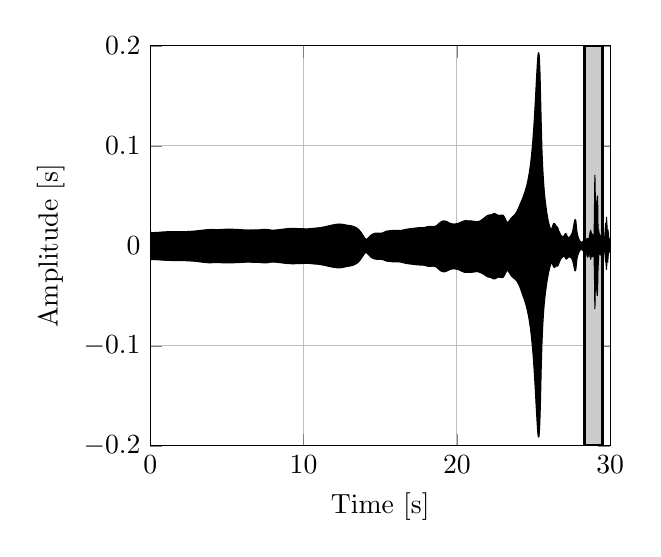
\begin{tikzpicture}

\begin{axis}[%
width=2.3in,
height=2in,
at={(1.011in,0.642in)},
scale only axis,
xmin=0,
xmax=30,
xmajorgrids,
ymin=-0.2,
ymax=0.2,
ymajorgrids,
xlabel={Time [s]},
ylabel={Amplitude [s]},
axis background/.style={fill=white}
]
\node[rectangle,draw, fill=black!20, minimum height=2in, minimum width=1pt, line width=1pt] at (axis cs:28.9,0) {};
\addplot[fill=black,draw=black,forget plot] plot table[row sep=crcr]{%
2.08333333333333e-05	0.0174441337585449\\
0.0250416666666667	0.013525128364563\\
0.0500625	0.013148307800293\\
0.0750833333333333	0.0131036043167114\\
0.100104166666667	0.0130690336227417\\
0.125125	0.0130878686904907\\
0.150145833333333	0.0131148099899292\\
0.175166666666667	0.0131456851959229\\
0.2001875	0.0131820440292358\\
0.225208333333333	0.0131937265396118\\
0.250229166666667	0.013242244720459\\
0.27525	0.0132321119308472\\
0.300270833333333	0.0132625102996826\\
0.325291666666667	0.0132992267608643\\
0.3503125	0.0133000612258911\\
0.375333333333333	0.0133060216903687\\
0.400354166666667	0.0133442878723145\\
0.425375	0.0133682489395142\\
0.450395833333333	0.0134040117263794\\
0.475416666666667	0.0134208202362061\\
0.5004375	0.0134366750717163\\
0.525458333333333	0.0134779214859009\\
0.550479166666667	0.013481616973877\\
0.5755	0.0135024785995483\\
0.600520833333333	0.0135313272476196\\
0.625541666666667	0.0135687589645386\\
0.6505625	0.0135985612869263\\
0.675583333333333	0.013633131980896\\
0.700604166666667	0.0136561393737793\\
0.725625	0.0136919021606445\\
0.750645833333333	0.0137306451797485\\
0.775666666666667	0.0137556791305542\\
0.8006875	0.01378333568573\\
0.825708333333333	0.0138041973114014\\
0.850729166666667	0.0138405561447144\\
0.87575	0.0138554573059082\\
0.900770833333333	0.0138554573059082\\
0.925791666666667	0.0138950347900391\\
0.9508125	0.0139113664627075\\
0.975833333333333	0.0139317512512207\\
1.00085416666667	0.0139557123184204\\
1.025875	0.0139747858047485\\
1.05089583333333	0.0140010118484497\\
1.07591666666667	0.0140320062637329\\
1.1009375	0.0140565633773804\\
1.12595833333333	0.0140770673751831\\
1.15097916666667	0.0140986442565918\\
1.176	0.0141662359237671\\
1.20102083333333	0.0141526460647583\\
1.22604166666667	0.0141149759292603\\
1.2510625	0.0141333341598511\\
1.27608333333333	0.0141546726226807\\
1.30110416666667	0.0141855478286743\\
1.326125	0.014235258102417\\
1.35114583333333	0.0142221450805664\\
1.37616666666667	0.0142310857772827\\
1.4011875	0.0142514705657959\\
1.42620833333333	0.0142489671707153\\
1.45122916666667	0.0142501592636108\\
1.47625	0.0142405033111572\\
1.50127083333333	0.0142426490783691\\
1.52629166666667	0.014230489730835\\
1.5513125	0.0142196416854858\\
1.57633333333333	0.0141897201538086\\
1.60135416666667	0.0141717195510864\\
1.626375	0.0141717195510864\\
1.65139583333333	0.0141562223434448\\
1.67641666666667	0.0141308307647705\\
1.7014375	0.0141433477401733\\
1.72645833333333	0.0141233205795288\\
1.75147916666667	0.0141158103942871\\
1.7765	0.0141146183013916\\
1.80152083333333	0.0140886306762695\\
1.82654166666667	0.0140882730484009\\
1.8515625	0.0140790939331055\\
1.87658333333333	0.0140920877456665\\
1.90160416666667	0.0140787363052368\\
1.926625	0.0140824317932129\\
1.95164583333333	0.014080286026001\\
1.97666666666667	0.0140800476074219\\
2.0016875	0.0140819549560547\\
2.02670833333333	0.0140724182128906\\
2.05172916666667	0.0140804052352905\\
2.07675	0.0140852928161621\\
2.10177083333333	0.0140907764434814\\
2.12679166666667	0.0141453742980957\\
2.1518125	0.0141433477401733\\
2.17683333333333	0.0141167640686035\\
2.20185416666667	0.014110803604126\\
2.226875	0.014117956161499\\
2.25189583333333	0.0141313076019287\\
2.27691666666667	0.01416015625\\
2.3019375	0.0141942501068115\\
2.32695833333333	0.0142010450363159\\
2.35197916666667	0.0142147541046143\\
2.377	0.0142277479171753\\
2.40202083333333	0.014255166053772\\
2.42704166666667	0.0142706632614136\\
2.4520625	0.0142948627471924\\
2.47708333333333	0.0143097639083862\\
2.50210416666667	0.014333963394165\\
2.527125	0.0143415927886963\\
2.55214583333333	0.0143803358078003\\
2.57716666666667	0.0144015550613403\\
2.6021875	0.0144282579421997\\
2.62720833333333	0.0144572257995605\\
2.65222916666667	0.0144776105880737\\
2.67725	0.0145164728164673\\
2.70227083333333	0.0145268440246582\\
2.72729166666667	0.0144838094711304\\
2.7523125	0.0145807266235352\\
2.77733333333333	0.0146057605743408\\
2.80235416666667	0.014631986618042\\
2.827375	0.0146661996841431\\
2.85239583333333	0.0147078037261963\\
2.87741666666667	0.0147354602813721\\
2.9024375	0.0147578716278076\\
2.92745833333333	0.0148038864135742\\
2.95247916666667	0.0148260593414307\\
2.9775	0.0148706436157227\\
3.00252083333333	0.0148930549621582\\
3.02754166666667	0.0149344205856323\\
3.0525625	0.0149737596511841\\
3.07758333333333	0.0150246620178223\\
3.10260416666667	0.0150657892227173\\
3.127625	0.0151075124740601\\
3.15264583333333	0.0151689052581787\\
3.17766666666667	0.0152368545532227\\
3.2026875	0.0152426958084106\\
3.22770833333333	0.0153077840805054\\
3.25272916666667	0.0153446197509766\\
3.27775	0.0153803825378418\\
3.30277083333333	0.0154129266738892\\
3.32779166666667	0.0154589414596558\\
3.3528125	0.0155411958694458\\
3.37783333333333	0.0155452489852905\\
3.40285416666667	0.0155919790267944\\
3.427875	0.0156158208847046\\
3.45289583333333	0.0156674385070801\\
3.47791666666667	0.0156955718994141\\
3.5029375	0.0157450437545776\\
3.52795833333333	0.0157967805862427\\
3.55297916666667	0.0158439874649048\\
3.578	0.0158843994140625\\
3.60302083333333	0.0159142017364502\\
3.62804166666667	0.0159745216369629\\
3.6530625	0.0160062313079834\\
3.67808333333333	0.0160480737686157\\
3.70310416666667	0.0160622596740723\\
3.728125	0.0160926580429077\\
3.75314583333333	0.0161361694335938\\
3.77816666666667	0.0161548852920532\\
3.8031875	0.0161689519882202\\
3.82820833333333	0.0162111520767212\\
3.85322916666667	0.0162196159362793\\
3.87825	0.0162382125854492\\
3.90327083333333	0.0162340402603149\\
3.92829166666667	0.0162550210952759\\
3.9533125	0.0162825584411621\\
3.97833333333333	0.016268253326416\\
4.00335416666667	0.0162605047225952\\
4.028375	0.0162662267684937\\
4.05339583333333	0.0162646770477295\\
4.07841666666667	0.0162562131881714\\
4.1034375	0.0162479877471924\\
4.12845833333333	0.0162286758422852\\
4.15347916666667	0.0162270069122314\\
4.1785	0.0162371397018433\\
4.20352083333333	0.0162290334701538\\
4.22854166666667	0.0162320137023926\\
4.2535625	0.0162011384963989\\
4.27858333333333	0.0161998271942139\\
4.30360416666667	0.0161756277084351\\
4.328625	0.0161881446838379\\
4.35364583333333	0.0161887407302856\\
4.37866666666667	0.0161789655685425\\
4.4036875	0.0161731243133545\\
4.42870833333333	0.0161886215209961\\
4.45372916666667	0.0162254571914673\\
4.47875	0.0162070989608765\\
4.50377083333333	0.0162215232849121\\
4.52879166666667	0.0162445306777954\\
4.5538125	0.0162478685379028\\
4.57883333333333	0.0162779092788696\\
4.60385416666667	0.0163146257400513\\
4.628875	0.0163321495056152\\
4.65389583333333	0.0163751840591431\\
4.67891666666667	0.0163940191268921\\
4.7039375	0.0164142847061157\\
4.72895833333333	0.0164343118667603\\
4.75397916666667	0.0164676904678345\\
4.779	0.0164873600006104\\
4.80402083333333	0.0164920091629028\\
4.82904166666667	0.0165045261383057\\
4.8540625	0.0165075063705444\\
4.87908333333333	0.0164927244186401\\
4.90410416666667	0.0165128707885742\\
4.929125	0.0165145397186279\\
4.95414583333333	0.0165392160415649\\
4.97916666666667	0.0165292024612427\\
5.0041875	0.0165307521820068\\
5.02920833333333	0.0165344476699829\\
5.05422916666667	0.0165383815765381\\
5.07925	0.0165324211120605\\
5.10427083333333	0.0165327787399292\\
5.12929166666667	0.0165436267852783\\
5.1543125	0.0165482759475708\\
5.17933333333333	0.0165408849716187\\
5.20435416666667	0.0165520906448364\\
5.229375	0.0165524482727051\\
5.25439583333333	0.0165770053863525\\
5.27941666666667	0.0165494680404663\\
5.3044375	0.0165427923202515\\
5.32945833333333	0.0165486335754395\\
5.35447916666667	0.016539454460144\\
5.3795	0.0165292024612427\\
5.40452083333333	0.0165024995803833\\
5.42954166666667	0.0165091753005981\\
5.4545625	0.0165070295333862\\
5.47958333333333	0.0164998769760132\\
5.50460416666667	0.0164941549301147\\
5.529625	0.0164831876754761\\
5.55464583333333	0.0164557695388794\\
5.57966666666667	0.0164422988891602\\
5.6046875	0.0164165496826172\\
5.62970833333333	0.0164107084274292\\
5.65472916666667	0.0163847208023071\\
5.67975	0.0163700580596924\\
5.70477083333333	0.0163614749908447\\
5.72979166666667	0.0163367986679077\\
5.7548125	0.0162984132766724\\
5.77983333333333	0.0162603855133057\\
5.80485416666667	0.0162379741668701\\
5.829875	0.0161999464035034\\
5.85489583333333	0.0161981582641602\\
5.87991666666667	0.0161627531051636\\
5.9049375	0.0161465406417847\\
5.92995833333333	0.016115665435791\\
5.95497916666667	0.0160897970199585\\
5.98	0.0160585641860962\\
6.00502083333333	0.0160255432128906\\
6.03004166666667	0.0159686803817749\\
6.0550625	0.0159963369369507\\
6.08008333333333	0.0159759521484375\\
6.10510416666667	0.0159282684326172\\
6.130125	0.015892505645752\\
6.15514583333333	0.0158891677856445\\
6.18016666666667	0.0158644914627075\\
6.2051875	0.0158466100692749\\
6.23020833333333	0.0158360004425049\\
6.25522916666667	0.0158376693725586\\
6.28025	0.0158051252365112\\
6.30527083333333	0.0157734155654907\\
6.33029166666667	0.0157642364501953\\
6.3553125	0.015750527381897\\
6.38033333333333	0.0157539844512939\\
6.40535416666667	0.0157500505447388\\
6.430375	0.0157680511474609\\
6.45539583333333	0.0157589912414551\\
6.48041666666667	0.0157626867294312\\
6.5054375	0.0157822370529175\\
6.53045833333333	0.0157740116119385\\
6.55547916666667	0.0157889127731323\\
6.5805	0.01578688621521\\
6.60552083333333	0.0157822370529175\\
6.63054166666667	0.015788197517395\\
6.6555625	0.0157915353775024\\
6.68058333333333	0.0158027410507202\\
6.70560416666667	0.0158090591430664\\
6.730625	0.0157994031906128\\
6.75564583333333	0.0158072710037231\\
6.78066666666667	0.0158181190490723\\
6.8056875	0.0157982110977173\\
6.83070833333333	0.0158140659332275\\
6.85572916666667	0.0158218145370483\\
6.88075	0.0158369541168213\\
6.90577083333333	0.015845775604248\\
6.93079166666667	0.0158636569976807\\
6.9558125	0.0158761739730835\\
6.98083333333333	0.0158882141113281\\
7.00585416666667	0.0158886909484863\\
7.030875	0.015921950340271\\
7.05589583333333	0.015964150428772\\
7.08091666666667	0.0159696340560913\\
7.1059375	0.0159767866134644\\
7.13095833333333	0.0160138607025146\\
7.15597916666667	0.0160485506057739\\
7.181	0.0161073207855225\\
7.20602083333333	0.0161236524581909\\
7.23104166666667	0.0161528587341309\\
7.2560625	0.0162006616592407\\
7.28108333333333	0.0162516832351685\\
7.30610416666667	0.0162925720214844\\
7.331125	0.0163209438323975\\
7.35614583333333	0.0163383483886719\\
7.38116666666667	0.0163733959197998\\
7.4061875	0.0163830518722534\\
7.43120833333333	0.0164109468460083\\
7.45622916666667	0.0164159536361694\\
7.48125	0.0164202451705933\\
7.50627083333333	0.01641845703125\\
7.53129166666667	0.0163898468017578\\
7.5563125	0.0163893699645996\\
7.58133333333333	0.0163614749908447\\
7.60635416666667	0.0163397789001465\\
7.631375	0.016291618347168\\
7.65639583333333	0.0162471532821655\\
7.68141666666667	0.0162198543548584\\
7.7064375	0.016148567199707\\
7.73145833333333	0.0160896778106689\\
7.75647916666667	0.016048789024353\\
7.7815	0.0159863233566284\\
7.80652083333333	0.0158941745758057\\
7.83154166666667	0.0158556699752808\\
7.8565625	0.0158106088638306\\
7.88158333333333	0.0157514810562134\\
7.90660416666667	0.0157146453857422\\
7.931625	0.0156705379486084\\
7.95664583333333	0.015657901763916\\
7.98166666666667	0.0156430006027222\\
8.0066875	0.015637993812561\\
8.03170833333333	0.0156441926956177\\
8.05672916666667	0.015630841255188\\
8.08175	0.0156583786010742\\
8.10677083333333	0.0156680345535278\\
8.13179166666667	0.0156958103179932\\
8.1568125	0.0157588720321655\\
8.18183333333333	0.0157665014266968\\
8.20685416666667	0.015811562538147\\
8.231875	0.0158299207687378\\
8.25689583333333	0.0158756971359253\\
8.28191666666667	0.0159240961074829\\
8.3069375	0.0159738063812256\\
8.33195833333333	0.0160108804702759\\
8.35697916666667	0.01605224609375\\
8.382	0.0161123275756836\\
8.40702083333333	0.0161582231521606\\
8.43204166666667	0.0161970853805542\\
8.4570625	0.0162638425827026\\
8.48208333333333	0.0163058042526245\\
8.50710416666667	0.0163264274597168\\
8.532125	0.0163748264312744\\
8.55714583333333	0.016425609588623\\
8.58216666666667	0.0164724588394165\\
8.6071875	0.0164806842803955\\
8.63220833333333	0.0165771245956421\\
8.65722916666667	0.0166155099868774\\
8.68225	0.0166538953781128\\
8.70727083333333	0.0166980028152466\\
8.73229166666667	0.0167548656463623\\
8.7573125	0.0168157815933228\\
8.78233333333333	0.0168620347976685\\
8.80735416666667	0.0168946981430054\\
8.832375	0.0169271230697632\\
8.85739583333333	0.0169821977615356\\
8.88241666666667	0.0170294046401978\\
8.9074375	0.0170701742172241\\
8.93245833333333	0.0171375274658203\\
8.95747916666667	0.0171374082565308\\
8.9825	0.0171587467193604\\
9.00752083333333	0.0172109603881836\\
9.03254166666667	0.017237663269043\\
9.0575625	0.0172935724258423\\
9.08258333333333	0.0173063278198242\\
9.10760416666667	0.0173218250274658\\
9.132625	0.0173497200012207\\
9.15764583333333	0.0173478126525879\\
9.18266666666667	0.0173822641372681\\
9.2076875	0.0173777341842651\\
9.23270833333333	0.0174020528793335\\
9.25772916666667	0.0174028873443604\\
9.28275	0.0174024105072021\\
9.30777083333333	0.0174020528793335\\
9.33279166666667	0.017372727394104\\
9.3578125	0.017397403717041\\
9.38283333333333	0.017382025718689\\
9.40785416666667	0.0173285007476807\\
9.432875	0.017330527305603\\
9.45789583333333	0.0173323154449463\\
9.48291666666667	0.0173298120498657\\
9.5079375	0.0173071622848511\\
9.53295833333333	0.0172946453094482\\
9.55797916666667	0.0172981023788452\\
9.583	0.0172525644302368\\
9.60802083333333	0.0172533988952637\\
9.63304166666667	0.0172268152236938\\
9.6580625	0.0172150135040283\\
9.68308333333333	0.0172126293182373\\
9.70810416666667	0.0172011852264404\\
9.733125	0.0171859264373779\\
9.75814583333333	0.0171804428100586\\
9.78316666666667	0.0171525478363037\\
9.8081875	0.0171377658843994\\
9.83320833333334	0.0171386003494263\\
9.85822916666667	0.0171124935150146\\
9.88325	0.0171166658401489\\
9.90827083333333	0.0170993804931641\\
9.93329166666667	0.0170944929122925\\
9.9583125	0.0170706510543823\\
9.98333333333333	0.0170501470565796\\
10.0083541666667	0.0170356035232544\\
10.033375	0.0169914960861206\\
10.0583958333333	0.0170005559921265\\
10.0834166666667	0.0170102119445801\\
10.1084375	0.0169705152511597\\
10.1334583333333	0.0169491767883301\\
10.1584791666667	0.0169483423233032\\
10.1835	0.0169246196746826\\
10.2085208333333	0.0169349908828735\\
10.2335416666667	0.016913890838623\\
10.2585625	0.016938328742981\\
10.2835833333333	0.0169572830200195\\
10.3086041666667	0.0169775485992432\\
10.333625	0.016999363899231\\
10.3586458333333	0.0170327425003052\\
10.3836666666667	0.0170744657516479\\
10.4086875	0.0170915126800537\\
10.4337083333333	0.0171260833740234\\
10.4587291666667	0.0171712636947632\\
10.48375	0.0172317028045654\\
10.5087708333333	0.0172442197799683\\
10.5337916666667	0.0172771215438843\\
10.5588125	0.017345666885376\\
10.5838333333333	0.0173889398574829\\
10.6088541666667	0.0174278020858765\\
10.633875	0.0174736976623535\\
10.6588958333333	0.0175179243087769\\
10.6839166666667	0.017504096031189\\
10.7089375	0.0175975561141968\\
10.7339583333333	0.0176342725753784\\
10.7589791666667	0.0176651477813721\\
10.784	0.0177170038223267\\
10.8090208333333	0.0177382230758667\\
10.8340416666667	0.0177578926086426\\
10.8590625	0.0177834033966064\\
10.8840833333333	0.0178287029266357\\
10.9091041666667	0.0178596973419189\\
10.934125	0.0178934335708618\\
10.9591458333333	0.0179351568222046\\
10.9841666666667	0.0179930925369263\\
11.0091875	0.0180190801620483\\
11.0342083333333	0.0180590152740479\\
11.0592291666667	0.0180873870849609\\
11.08425	0.0181617736816406\\
11.1092708333333	0.0181983709335327\\
11.1342916666667	0.0182547569274902\\
11.1593125	0.018323540687561\\
11.1843333333333	0.018383264541626\\
11.2093541666667	0.0184645652770996\\
11.234375	0.0185511112213135\\
11.2593958333333	0.0186281204223633\\
11.2844166666667	0.0186648368835449\\
11.3094375	0.0187809467315674\\
11.3344583333333	0.0188539028167725\\
11.3594791666667	0.0189625024795532\\
11.3845	0.0190408229827881\\
11.4095208333333	0.0191167593002319\\
11.4345416666667	0.0191928148269653\\
11.4595625	0.019289493560791\\
11.4845833333333	0.0194246768951416\\
11.5096041666667	0.0194790363311768\\
11.534625	0.0195668935775757\\
11.5596458333333	0.0196346044540405\\
11.5846666666667	0.0197362899780273\\
11.6096875	0.0198198556900024\\
11.6347083333333	0.0198944807052612\\
11.6597291666667	0.0199992656707764\\
11.68475	0.0200852155685425\\
11.7097708333333	0.0201708078384399\\
11.7347916666667	0.0202442407608032\\
11.7598125	0.0203417539596558\\
11.7848333333333	0.020447850227356\\
11.8098541666667	0.0205179452896118\\
11.834875	0.020601749420166\\
11.8598958333333	0.0206559896469116\\
11.8849166666667	0.0207802057266235\\
11.9099375	0.0208553075790405\\
11.9349583333333	0.0209276676177979\\
11.9599791666667	0.0209884643554688\\
11.985	0.0210902690887451\\
12.0100208333333	0.0211566686630249\\
12.0350416666667	0.0212430953979492\\
12.0600625	0.0213093757629395\\
12.0850833333333	0.0213801860809326\\
12.1101041666667	0.0214052200317383\\
12.135125	0.0214844942092896\\
12.1601458333333	0.0215476751327515\\
12.1851666666667	0.0216346979141235\\
12.2101875	0.0216710567474365\\
12.2352083333333	0.0217214822769165\\
12.2602291666667	0.0217512845993042\\
12.28525	0.0217370986938477\\
12.3102708333333	0.0217386484146118\\
12.3352916666667	0.0217440128326416\\
12.3603125	0.0217629671096802\\
12.3853333333333	0.0217190980911255\\
12.4103541666667	0.0217164754867554\\
12.435375	0.0216363668441772\\
12.4603958333333	0.0216211080551147\\
12.4854166666667	0.021581768989563\\
12.5104375	0.0215216875076294\\
12.5354583333333	0.021467924118042\\
12.5604791666667	0.0213643312454224\\
12.5855	0.021304726600647\\
12.6105208333333	0.0212384462356567\\
12.6355416666667	0.0211762189865112\\
12.6605625	0.0210961103439331\\
12.6855833333333	0.0210355520248413\\
12.7106041666667	0.0209527015686035\\
12.735625	0.0208666324615479\\
12.7606458333333	0.0208185911178589\\
12.7856666666667	0.0207582712173462\\
12.8106875	0.0206890106201172\\
12.8357083333333	0.0206308364868164\\
12.8607291666667	0.0205554962158203\\
12.88575	0.0205261707305908\\
12.9107708333333	0.0204222202301025\\
12.9357916666667	0.0204188823699951\\
12.9608125	0.0203204154968262\\
12.9858333333333	0.0202691555023193\\
13.0108541666667	0.0202019214630127\\
13.035875	0.0201456546783447\\
13.0608958333333	0.0200655460357666\\
13.0859166666667	0.0200191736221313\\
13.1109375	0.0199253559112549\\
13.1359583333333	0.0198445320129395\\
13.1609791666667	0.0197505950927734\\
13.186	0.0197038650512695\\
13.2110208333333	0.0195786952972412\\
13.2360416666667	0.019476056098938\\
13.2610625	0.0193073749542236\\
13.2860833333333	0.0191764831542969\\
13.3111041666667	0.0190207958221436\\
13.336125	0.0188961029052734\\
13.3611458333333	0.0186749696731567\\
13.3861666666667	0.0185122489929199\\
13.4111875	0.0183169841766357\\
13.4362083333333	0.0180661678314209\\
13.4612291666667	0.017853856086731\\
13.48625	0.0175918340682983\\
13.5112708333333	0.0173110961914062\\
13.5362916666667	0.0169925689697266\\
13.5613125	0.0166597366333008\\
13.5863333333333	0.0163099765777588\\
13.6113541666667	0.0159174203872681\\
13.636375	0.0155293941497803\\
13.6613958333333	0.0150763988494873\\
13.6864166666667	0.0146143436431885\\
13.7114375	0.014168381690979\\
13.7364583333333	0.0136096477508545\\
13.7614791666667	0.0130655765533447\\
13.7865	0.0125436782836914\\
13.8115208333333	0.0119357109069824\\
13.8365416666667	0.0113338232040405\\
13.8615625	0.0106756687164307\\
13.8865833333333	0.0100915431976318\\
13.9116041666667	0.00947129726409912\\
13.936625	0.00886750221252441\\
13.9616458333333	0.00825822353363037\\
13.9866666666667	0.00778257846832275\\
14.0116875	0.00735759735107422\\
14.0367083333333	0.00696361064910889\\
14.0617291666667	0.00667524337768555\\
14.08675	0.00652050971984863\\
14.1117708333333	0.00652647018432617\\
14.1367916666667	0.00670945644378662\\
14.1618125	0.00699913501739502\\
14.1868333333333	0.00733792781829834\\
14.2118541666667	0.0077139139175415\\
14.236875	0.00815272331237793\\
14.2618958333333	0.00860869884490967\\
14.2869166666667	0.00900518894195557\\
14.3119375	0.00939702987670898\\
14.3369583333333	0.00978922843933105\\
14.3619791666667	0.0101321935653687\\
14.387	0.0104804039001465\\
14.4120208333333	0.0107772350311279\\
14.4370416666667	0.0110471248626709\\
14.4620625	0.0112928152084351\\
14.4870833333333	0.0115351676940918\\
14.5121041666667	0.0117450952529907\\
14.537125	0.0118981599807739\\
14.5621458333333	0.0120600461959839\\
14.5871666666667	0.0121918916702271\\
14.6121875	0.0123043060302734\\
14.6372083333333	0.0123888254165649\\
14.6622291666667	0.0124760866165161\\
14.68725	0.0125365257263184\\
14.7122708333333	0.0126163959503174\\
14.7372916666667	0.0126279592514038\\
14.7623125	0.0126475095748901\\
14.7873333333333	0.0126579999923706\\
14.8123541666667	0.0126771926879883\\
14.837375	0.0126643180847168\\
14.8623958333333	0.0126522779464722\\
14.8874166666667	0.0126442909240723\\
14.9124375	0.0126438140869141\\
14.9374583333333	0.0126296281814575\\
14.9624791666667	0.0126005411148071\\
14.9875	0.0125808715820312\\
15.0125208333333	0.0125870704650879\\
15.0375416666667	0.0125871896743774\\
15.0625625	0.0126022100448608\\
15.0875833333333	0.0126547813415527\\
15.1126041666667	0.0127360820770264\\
15.137625	0.0128141641616821\\
15.1626458333333	0.0129730701446533\\
15.1876666666667	0.0131022930145264\\
15.2126875	0.0132739543914795\\
15.2377083333333	0.0134528875350952\\
15.2627291666667	0.0136306285858154\\
15.28775	0.0138425827026367\\
15.3127708333333	0.0140299797058105\\
15.3377916666667	0.014187216758728\\
15.3628125	0.0143324136734009\\
15.3878333333333	0.0144814252853394\\
15.4128541666667	0.0145851373672485\\
15.437875	0.0147069692611694\\
15.4628958333333	0.0147304534912109\\
15.4879166666667	0.014826774597168\\
15.5129375	0.0148801803588867\\
15.5379583333333	0.0149414539337158\\
15.5629791666667	0.0149836540222168\\
15.588	0.0150250196456909\\
15.6130208333333	0.0150867700576782\\
15.6380416666667	0.0151267051696777\\
15.6630625	0.0151498317718506\\
15.6880833333333	0.0151907205581665\\
15.7131041666667	0.0152368545532227\\
15.738125	0.0152875185012817\\
15.7631458333333	0.0153127908706665\\
15.7881666666667	0.015317440032959\\
15.8131875	0.0153570175170898\\
15.8382083333333	0.0153809785842896\\
15.8632291666667	0.0153845548629761\\
15.88825	0.0154021978378296\\
15.9132708333333	0.0154201984405518\\
15.9382916666667	0.0154287815093994\\
15.9633125	0.0154200792312622\\
15.9883333333333	0.0154142379760742\\
16.0133541666667	0.0154227018356323\\
16.038375	0.0153951644897461\\
16.0633958333333	0.0153549909591675\\
16.0884166666667	0.0153504610061646\\
16.1134375	0.015299916267395\\
16.1384583333333	0.0152820348739624\\
16.1634791666667	0.0152640342712402\\
16.1885	0.0152740478515625\\
16.2135208333333	0.0152524709701538\\
16.2385416666667	0.0152736902236938\\
16.2635625	0.0152624845504761\\
16.2885833333333	0.0152912139892578\\
16.3136041666667	0.0153496265411377\\
16.338625	0.015373706817627\\
16.3636458333333	0.0154263973236084\\
16.3886666666667	0.0154972076416016\\
16.4136875	0.0155841112136841\\
16.4387083333333	0.0156378746032715\\
16.4637291666667	0.01569664478302\\
16.48875	0.015790581703186\\
16.5137708333333	0.0158723592758179\\
16.5387916666667	0.0159751176834106\\
16.5638125	0.0160551071166992\\
16.5888333333333	0.0161577463150024\\
16.6138541666667	0.0162507295608521\\
16.638875	0.0163224935531616\\
16.6638958333333	0.0163685083389282\\
16.6889166666667	0.0164364576339722\\
16.7139375	0.0165036916732788\\
16.7389583333333	0.0165603160858154\\
16.7639791666667	0.0166410207748413\\
16.789	0.0167248249053955\\
16.8140208333333	0.0167744159698486\\
16.8390416666667	0.016828179359436\\
16.8640625	0.0168788433074951\\
16.8890833333333	0.0169576406478882\\
16.9141041666667	0.016994833946228\\
16.939125	0.0170410871505737\\
16.9641458333333	0.0170806646347046\\
16.9891666666667	0.017139196395874\\
17.0141875	0.0172109603881836\\
17.0392083333333	0.0172618627548218\\
17.0642291666667	0.0173348188400269\\
17.08925	0.0173755884170532\\
17.1142708333333	0.0174448490142822\\
17.1392916666667	0.0174486637115479\\
17.1643125	0.0174803733825684\\
17.1893333333333	0.017526388168335\\
17.2143541666667	0.0175930261611938\\
17.239375	0.0176322460174561\\
17.2643958333333	0.0176610946655273\\
17.2894166666667	0.0177028179168701\\
17.3144375	0.0177712440490723\\
17.3394583333333	0.017817497253418\\
17.3644791666667	0.0178496837615967\\
17.3895	0.0178635120391846\\
17.4145208333333	0.0179288387298584\\
17.4395416666667	0.017961859703064\\
17.4645625	0.017999529838562\\
17.4895833333333	0.018022894859314\\
17.5146041666667	0.018062949180603\\
17.539625	0.0180728435516357\\
17.5646458333333	0.01810622215271\\
17.5896666666667	0.0180763006210327\\
17.6146875	0.0180631875991821\\
17.6397083333333	0.0180815458297729\\
17.6647291666667	0.0180732011795044\\
17.68975	0.0180611610412598\\
17.7147708333333	0.0180732011795044\\
17.7397916666667	0.0180991888046265\\
17.7648125	0.018126368522644\\
17.7898333333333	0.0181397199630737\\
17.8148541666667	0.0181893110275269\\
17.839875	0.0182832479476929\\
17.8648958333333	0.0183231830596924\\
17.8899166666667	0.0183992385864258\\
17.9149375	0.0184700489044189\\
17.9399583333333	0.0185521841049194\\
17.9649791666667	0.0186257362365723\\
17.99	0.0187492370605469\\
18.0150208333333	0.0188664197921753\\
18.0400416666667	0.0189815759658813\\
18.0650625	0.0190328359603882\\
18.0900833333333	0.0191329717636108\\
18.1151041666667	0.0192264318466187\\
18.140125	0.0192656517028809\\
18.1651458333333	0.0192974805831909\\
18.1901666666667	0.0193121433258057\\
18.2151875	0.0193363428115845\\
18.2402083333333	0.0193533897399902\\
18.2652291666667	0.0193248987197876\\
18.29025	0.0193346738815308\\
18.3152708333333	0.0193099975585938\\
18.3402916666667	0.0192739963531494\\
18.3653125	0.0192720890045166\\
18.3903333333333	0.0192562341690063\\
18.4153541666667	0.0192611217498779\\
18.440375	0.0192636251449585\\
18.4653958333333	0.0192465782165527\\
18.4904166666667	0.0192739963531494\\
18.5154375	0.0192666053771973\\
18.5404583333333	0.0192996263504028\\
18.5654791666667	0.0193842649459839\\
18.5905	0.0194982290267944\\
18.6155208333333	0.0196996927261353\\
18.6405416666667	0.0198712348937988\\
18.6655625	0.0201015472412109\\
18.6905833333333	0.02039635181427\\
18.7156041666667	0.0207115411758423\\
18.740625	0.02104651927948\\
18.7656458333333	0.0213632583618164\\
18.7906666666667	0.0217374563217163\\
18.8156875	0.0221004486083984\\
18.8407083333333	0.0224542617797852\\
18.8657291666667	0.0227910280227661\\
18.89075	0.023115873336792\\
18.9157708333333	0.0234055519104004\\
18.9407916666667	0.0236350297927856\\
18.9658125	0.0238840579986572\\
18.9908333333333	0.0240856409072876\\
19.0158541666667	0.0243097543716431\\
19.040875	0.0244883298873901\\
19.0658958333333	0.0246367454528809\\
19.0909166666667	0.0247553586959839\\
19.1159375	0.0248157978057861\\
19.1409583333333	0.0248211622238159\\
19.1659791666667	0.0248291492462158\\
19.191	0.0247656106948853\\
19.2160208333333	0.0247126817703247\\
19.2410416666667	0.0246188640594482\\
19.2660625	0.0245308876037598\\
19.2910833333333	0.024416446685791\\
19.3161041666667	0.0243091583251953\\
19.341125	0.0241603851318359\\
19.3661458333333	0.0239905118942261\\
19.3911666666667	0.0237839221954346\\
19.4161875	0.0236095190048218\\
19.4412083333333	0.0234092473983765\\
19.4662291666667	0.0231764316558838\\
19.49125	0.0229754447937012\\
19.5162708333333	0.022815465927124\\
19.5412916666667	0.0226483345031738\\
19.5663125	0.0224692821502686\\
19.5913333333333	0.0223290920257568\\
19.6163541666667	0.0222113132476807\\
19.641375	0.0221070051193237\\
19.6663958333333	0.0220341682434082\\
19.6914166666667	0.0219175815582275\\
19.7164375	0.0218663215637207\\
19.7414583333333	0.0218421220779419\\
19.7664791666667	0.0217581987380981\\
19.7915	0.021744966506958\\
19.8165208333333	0.0217596292495728\\
19.8415416666667	0.0217770338058472\\
19.8665625	0.0217828750610352\\
19.8915833333333	0.0218362808227539\\
19.9166041666667	0.0218791961669922\\
19.941625	0.0219467878341675\\
19.9666458333333	0.0220240354537964\\
19.9916666666667	0.0220874547958374\\
20.0166875	0.0221959352493286\\
20.0417083333333	0.022313117980957\\
20.0667291666667	0.0224117040634155\\
20.09175	0.0225427150726318\\
20.1167708333333	0.0226690769195557\\
20.1417916666667	0.0228263139724731\\
20.1668125	0.0229573249816895\\
20.1918333333333	0.0231013298034668\\
20.2168541666667	0.0232757329940796\\
20.241875	0.0234352350234985\\
20.2668958333333	0.0236291885375977\\
20.2919166666667	0.0237768888473511\\
20.3169375	0.023958683013916\\
20.3419583333333	0.0241364240646362\\
20.3669791666667	0.0242964029312134\\
20.392	0.0244518518447876\\
20.4170208333333	0.0246180295944214\\
20.4420416666667	0.0247514247894287\\
20.4670625	0.0248813629150391\\
20.4920833333333	0.0249801874160767\\
20.5171041666667	0.0250335931777954\\
20.542125	0.0250766277313232\\
20.5671458333333	0.0250948667526245\\
20.5921666666667	0.0251015424728394\\
20.6171875	0.0250868797302246\\
20.6422083333333	0.025084376335144\\
20.6672291666667	0.0250357389450073\\
20.69225	0.0249865055084229\\
20.7172708333333	0.0249638557434082\\
20.7422916666667	0.0249263048171997\\
20.7673125	0.0249083042144775\\
20.7923333333333	0.0248900651931763\\
20.8173541666667	0.0248545408248901\\
20.842375	0.0248538255691528\\
20.8673958333333	0.0248371362686157\\
20.8924166666667	0.0248321294784546\\
20.9174375	0.0248321294784546\\
20.9424583333333	0.0248123407363892\\
20.9674791666667	0.0248016119003296\\
20.9925	0.0247378349304199\\
21.0175208333333	0.0246872901916504\\
21.0425416666667	0.0246568918228149\\
21.0675625	0.0245620012283325\\
21.0925833333333	0.0245187282562256\\
21.1176041666667	0.0244406461715698\\
21.142625	0.0243560075759888\\
21.1676458333333	0.0242875814437866\\
21.1926666666667	0.0241986513137817\\
21.2176875	0.0241419076919556\\
21.2427083333333	0.0241051912307739\\
21.2677291666667	0.0240743160247803\\
21.29275	0.0240596532821655\\
21.3177708333333	0.0240672826766968\\
21.3427916666667	0.0241365432739258\\
21.3678125	0.0242211818695068\\
21.3928333333333	0.0242770910263062\\
21.4178541666667	0.0243664979934692\\
21.442875	0.0245187282562256\\
21.4678958333333	0.0246692895889282\\
21.4929166666667	0.0248323678970337\\
21.5179375	0.0250157117843628\\
21.5429583333333	0.0251970291137695\\
21.5679791666667	0.0254095792770386\\
21.593	0.0256576538085938\\
21.6180208333333	0.0259164571762085\\
21.6430416666667	0.0261667966842651\\
21.6680625	0.0264409780502319\\
21.6930833333333	0.0267170667648315\\
21.7181041666667	0.0269858837127686\\
21.743125	0.0273033380508423\\
21.7681458333333	0.0276157855987549\\
21.7931666666667	0.0278679132461548\\
21.8181875	0.0282278060913086\\
21.8432083333333	0.0285413265228271\\
21.8682291666667	0.0288461446762085\\
21.89325	0.029139518737793\\
21.9182708333333	0.0294617414474487\\
21.9432916666667	0.0297086238861084\\
21.9683125	0.0300043821334839\\
21.9933333333333	0.0302213430404663\\
22.0183541666667	0.0304399728775024\\
22.043375	0.0305919647216797\\
22.0683958333333	0.0306967496871948\\
22.0934166666667	0.0307843685150146\\
22.1184375	0.0307987928390503\\
22.1434583333333	0.030825138092041\\
22.1684791666667	0.0308159589767456\\
22.1935	0.0308229923248291\\
22.2185208333333	0.0309444665908813\\
22.2435416666667	0.0311071872711182\\
22.2685625	0.0312448740005493\\
22.2935833333333	0.0314546823501587\\
22.3186041666667	0.0316667556762695\\
22.343625	0.0318219661712646\\
22.3686458333333	0.0320000648498535\\
22.3936666666667	0.0320919752120972\\
22.4186875	0.0321664810180664\\
22.4437083333333	0.0321915149688721\\
22.4687291666667	0.0321606397628784\\
22.49375	0.0321078300476074\\
22.5187708333333	0.031922459602356\\
22.5437916666667	0.0317248106002808\\
22.5688125	0.031496524810791\\
22.5938333333333	0.0312548875808716\\
22.6188541666667	0.0311131477355957\\
22.643875	0.0308171510696411\\
22.6688958333333	0.030713677406311\\
22.6939166666667	0.030561089515686\\
22.7189375	0.0304679870605469\\
22.7439583333333	0.0304421186447144\\
22.7689791666667	0.0303603410720825\\
22.794	0.0303953886032104\\
22.8190208333333	0.0304563045501709\\
22.8440416666667	0.0305156707763672\\
22.8690625	0.0305367708206177\\
22.8940833333333	0.0306057929992676\\
22.9191041666667	0.0306382179260254\\
22.944125	0.0306912660598755\\
22.9691458333333	0.0306316614151001\\
22.9941666666667	0.0306066274642944\\
23.0191875	0.0304591655731201\\
23.0442083333333	0.0300365686416626\\
23.0692291666667	0.0294849872589111\\
23.09425	0.0287594795227051\\
23.1192708333333	0.0279767513275146\\
23.1442916666667	0.027154803276062\\
23.1693125	0.0264017581939697\\
23.1943333333333	0.0256999731063843\\
23.2193541666667	0.0246617794036865\\
23.244375	0.0238051414489746\\
23.2693958333333	0.0236220359802246\\
23.2944166666667	0.0233170986175537\\
23.3194375	0.0234898328781128\\
23.3444583333333	0.0237802267074585\\
23.3694791666667	0.0241098403930664\\
23.3945	0.024639368057251\\
23.4195208333333	0.0251232385635376\\
23.4445416666667	0.0256147384643555\\
23.4695625	0.0261942148208618\\
23.4945833333333	0.0267441272735596\\
23.5196041666667	0.0272728204727173\\
23.544625	0.0277079343795776\\
23.5696458333333	0.0281523466110229\\
23.5946666666667	0.0285365581512451\\
23.6196875	0.0288980007171631\\
23.6447083333333	0.0291863679885864\\
23.6697291666667	0.0294959545135498\\
23.69475	0.029880166053772\\
23.7197708333333	0.0302121639251709\\
23.7447916666667	0.0305644273757935\\
23.7698125	0.0310232639312744\\
23.7948333333333	0.0315340757369995\\
23.8198541666667	0.0320580005645752\\
23.844875	0.0326471328735352\\
23.8698958333333	0.0332018136978149\\
23.8949166666667	0.0337858200073242\\
23.9199375	0.0345264673233032\\
23.9449583333333	0.0352761745452881\\
23.9699791666667	0.0361440181732178\\
23.995	0.0370364189147949\\
24.0200208333333	0.0377423763275146\\
24.0450416666667	0.0387363433837891\\
24.0700625	0.0396305322647095\\
24.0950833333333	0.0405175685882568\\
24.1201041666667	0.041479229927063\\
24.145125	0.0423545837402344\\
24.1701458333333	0.0432147979736328\\
24.1951666666667	0.044137716293335\\
24.2201875	0.0450013875961304\\
24.2452083333333	0.0459293127059937\\
24.2702291666667	0.0469129085540771\\
24.29525	0.0479274988174438\\
24.3202708333333	0.0489280223846436\\
24.3452916666667	0.0500307083129883\\
24.3703125	0.0510417222976685\\
24.3953333333333	0.052181601524353\\
24.4203541666667	0.0532969236373901\\
24.445375	0.0544567108154297\\
24.4703958333333	0.0556988716125488\\
24.4954166666667	0.056898832321167\\
24.5204375	0.0582900047302246\\
24.5454583333333	0.0596746206283569\\
24.5704791666667	0.0611917972564697\\
24.5955	0.0627651214599609\\
24.6205208333333	0.0645843744277954\\
24.6455416666667	0.0664654970169067\\
24.6705625	0.0684857368469238\\
24.6955833333333	0.0705987215042114\\
24.7206041666667	0.0729748010635376\\
24.745625	0.0752949714660645\\
24.7706458333333	0.0780850648880005\\
24.7956666666667	0.0809968709945679\\
24.8206875	0.084004282951355\\
24.8457083333333	0.0875474214553833\\
24.8707291666667	0.0909876823425293\\
24.89575	0.0951199531555176\\
24.9207708333333	0.0991923809051514\\
24.9457916666667	0.103655219078064\\
24.9708125	0.108772873878479\\
24.9958333333333	0.114107251167297\\
25.0208541666667	0.119699358940125\\
25.045875	0.125730037689209\\
25.0708958333333	0.132137656211853\\
25.0959166666667	0.139050245285034\\
25.1209375	0.146229147911072\\
25.1459583333333	0.153596758842468\\
25.1709791666667	0.161020040512085\\
25.196	0.168261528015137\\
25.2210208333333	0.175299406051636\\
25.2460416666667	0.181927919387817\\
25.2710625	0.187173366546631\\
25.2960833333333	0.191585659980774\\
25.3211041666667	0.192880272865295\\
25.346125	0.192724227905273\\
25.3711458333333	0.189618349075317\\
25.3961666666667	0.181955933570862\\
25.4211875	0.171445846557617\\
25.4462083333333	0.155550122261047\\
25.4712291666667	0.139785528182983\\
25.49625	0.123754620552063\\
25.5212708333333	0.109553933143616\\
25.5462916666667	0.0963232517242432\\
25.5713125	0.086665153503418\\
25.5963333333333	0.0784014463424683\\
25.6213541666667	0.071405291557312\\
25.646375	0.0651895999908447\\
25.6713958333333	0.0598506927490234\\
25.6964166666667	0.0547468662261963\\
25.7214375	0.050620436668396\\
25.7464583333333	0.0471398830413818\\
25.7714791666667	0.043710470199585\\
25.7965	0.0407135486602783\\
25.8215208333333	0.0378057956695557\\
25.8465416666667	0.0348886251449585\\
25.8715625	0.0322417020797729\\
25.8965833333333	0.0300600528717041\\
25.9216041666667	0.0277225971221924\\
25.946625	0.025759220123291\\
25.9716458333333	0.0239880084991455\\
25.9966666666667	0.0221370458602905\\
26.0216875	0.0206685066223145\\
26.0467083333333	0.0193742513656616\\
26.0717291666667	0.0183048248291016\\
26.09675	0.0174481868743896\\
26.1217708333333	0.0168154239654541\\
26.1467916666667	0.0165709257125854\\
26.1718125	0.0168967247009277\\
26.1968333333333	0.0176175832748413\\
26.2218541666667	0.0186170339584351\\
26.246875	0.0197421312332153\\
26.2718958333333	0.0208824872970581\\
26.2969166666667	0.0218906402587891\\
26.3219375	0.0222227573394775\\
26.3469583333333	0.0223579406738281\\
26.3719791666667	0.0221942663192749\\
26.397	0.0217078924179077\\
26.4220208333333	0.0209922790527344\\
26.4470416666667	0.0202728509902954\\
26.4720625	0.0196545124053955\\
26.4970833333333	0.0193988084793091\\
26.5221041666667	0.0191034078598022\\
26.547125	0.0187299251556396\\
26.5721458333333	0.0180537700653076\\
26.5971666666667	0.0168862342834473\\
26.6221875	0.015802264213562\\
26.6472083333333	0.0147438049316406\\
26.6722291666667	0.0138993263244629\\
26.69725	0.0131711959838867\\
26.7222708333333	0.0123679637908936\\
26.7472916666667	0.0115710496902466\\
26.7723125	0.0107738971710205\\
26.7973333333333	0.0101497173309326\\
26.8223541666667	0.00979006290435791\\
26.847375	0.00962471961975098\\
26.8723958333333	0.00949633121490479\\
26.8974166666667	0.00931215286254883\\
26.9224375	0.00916421413421631\\
26.9474583333333	0.00920677185058594\\
26.9724791666667	0.00953972339630127\\
26.9975	0.0102084875106812\\
27.0225208333333	0.0108667612075806\\
27.0475416666667	0.0115419626235962\\
27.0725625	0.0120722055435181\\
27.0975833333333	0.0121549367904663\\
27.1226041666667	0.0118545293807983\\
27.147625	0.0111083984375\\
27.1726458333333	0.0101121664047241\\
27.1976666666667	0.0093076229095459\\
27.2226875	0.00873386859893799\\
27.2477083333333	0.00842678546905518\\
27.2727291666667	0.00834882259368896\\
27.29775	0.00836217403411865\\
27.3227708333333	0.00848746299743652\\
27.3477916666667	0.00875973701477051\\
27.3728125	0.0090184211730957\\
27.3978333333333	0.00947034358978271\\
27.4228541666667	0.00991213321685791\\
27.447875	0.0106494426727295\\
27.4728958333333	0.0113028287887573\\
27.4979166666667	0.012182354927063\\
27.5229375	0.0131195783615112\\
27.5479583333333	0.0144155025482178\\
27.5729791666667	0.0162382125854492\\
27.598	0.0181559324264526\\
27.6230208333333	0.0203871726989746\\
27.6480416666667	0.0227947235107422\\
27.6730625	0.0248361825942993\\
27.6980833333333	0.0259034633636475\\
27.7231041666667	0.0261249542236328\\
27.748125	0.0256080627441406\\
27.7731458333333	0.0226942300796509\\
27.7981666666667	0.0178313255310059\\
27.8231875	0.0147879123687744\\
27.8482083333333	0.0123029947280884\\
27.8732291666667	0.0105404853820801\\
27.89825	0.00934135913848877\\
27.9232708333333	0.00792503356933594\\
27.9482916666667	0.00695645809173584\\
27.9733125	0.00611364841461182\\
27.9983333333333	0.00526881217956543\\
28.0233541666667	0.00476109981536865\\
28.048375	0.00428164005279541\\
28.0733958333333	0.00390028953552246\\
28.0984166666667	0.00352144241333008\\
28.1234375	0.00320971012115479\\
28.1484583333333	0.00320219993591309\\
28.1734791666667	0.00377941131591797\\
28.1985	0.0043492317199707\\
28.2235208333333	0.00466501712799072\\
28.2485416666667	0.00484251976013184\\
28.2735625	0.00487172603607178\\
28.2985833333333	0.00505399703979492\\
28.3236041666667	0.00524246692657471\\
28.348625	0.00562095642089844\\
28.3736458333333	0.00589895248413086\\
28.3986666666667	0.00605738162994385\\
28.4236875	0.00629270076751709\\
28.4487083333333	0.00658106803894043\\
28.4737291666667	0.00671696662902832\\
28.49875	0.00694727897644043\\
28.5237708333333	0.0074467658996582\\
28.5487916666667	0.00746893882751465\\
28.5738125	0.00671839714050293\\
28.5988333333333	0.00586915016174316\\
28.6238541666667	0.00598013401031494\\
28.648875	0.00930511951446533\\
28.6738958333333	0.0123151540756226\\
28.6989166666667	0.0111576318740845\\
28.7239375	0.0158895254135132\\
28.7489583333333	0.00994598865509033\\
28.7739791666667	0.0123809576034546\\
28.799	0.0107604265213013\\
28.8240208333333	0.00990724563598633\\
28.8490416666667	0.00613832473754883\\
28.8740625	0.0101600885391235\\
28.8990833333333	0.00902903079986572\\
28.9241041666667	0.00855207443237305\\
28.949125	0.00797700881958008\\
28.9741458333333	0.0380454063415527\\
28.9991666666667	0.0708549022674561\\
29.0241875	0.0490773916244507\\
29.0492083333333	0.0407736301422119\\
29.0742291666667	0.0349804162979126\\
29.09925	0.0337502956390381\\
29.1242708333333	0.0392665863037109\\
29.1492916666667	0.0477851629257202\\
29.1743125	0.0501984357833862\\
29.1993333333333	0.0208961963653564\\
29.2243541666667	0.0139025449752808\\
29.249375	0.0146907567977905\\
29.2743958333333	0.0124069452285767\\
29.2994166666667	0.0113190412521362\\
29.3244375	0.0109615325927734\\
29.3494583333333	0.00985002517700195\\
29.3744791666667	0.0061262845993042\\
29.3995	0.00371837615966797\\
29.4245208333333	0.00360357761383057\\
29.4495416666667	0.00346684455871582\\
29.4745625	0.0025477409362793\\
29.4995833333333	0.0020289421081543\\
29.5246041666667	0.0020139217376709\\
29.549625	0.00211250782012939\\
29.5746458333333	0.00222396850585938\\
29.5996666666667	0.00345098972320557\\
29.6246875	0.0047835111618042\\
29.6497083333333	0.0106549263000488\\
29.6747291666667	0.0167301893234253\\
29.69975	0.0227276086807251\\
29.7247708333333	0.00887835025787354\\
29.7497916666667	0.0288950204849243\\
29.7748125	0.0240693092346191\\
29.7998333333333	0.0165066719055176\\
29.8248541666667	0.0125565528869629\\
29.849875	0.0164783000946045\\
29.8748958333333	0.00610911846160889\\
29.8999166666667	0.00875699520111084\\
29.9249375	0.00352859497070312\\
29.9499583333333	0.00749635696411133\\
29.9749791666667	0.00196146965026855\\
30	0.00157845020294189\\
}
\closedcycle;
\addplot[fill=black,draw=black,forget plot] plot table[row sep=crcr]{%
2.08333333333333e-05	-0.0159932374954224\\
0.0250416666666667	-0.0138821601867676\\
0.0500625	-0.0136831998825073\\
0.0750833333333333	-0.0136609077453613\\
0.100104166666667	-0.0136864185333252\\
0.125125	-0.01369309425354\\
0.150145833333333	-0.0137081146240234\\
0.175166666666667	-0.0137027502059937\\
0.2001875	-0.0137165784835815\\
0.225208333333333	-0.0137177705764771\\
0.250229166666667	-0.0137324333190918\\
0.27525	-0.0137653350830078\\
0.300270833333333	-0.0137816667556763\\
0.325291666666667	-0.0137958526611328\\
0.3503125	-0.0138300657272339\\
0.375333333333333	-0.0138684511184692\\
0.400354166666667	-0.013879656791687\\
0.425375	-0.0138978958129883\\
0.450395833333333	-0.013921856880188\\
0.475416666666667	-0.0139497518539429\\
0.5004375	-0.0139772891998291\\
0.525458333333333	-0.0140053033828735\\
0.550479166666667	-0.0140323638916016\\
0.5755	-0.0140612125396729\\
0.600520833333333	-0.0140962600708008\\
0.625541666666667	-0.0141171216964722\\
0.6505625	-0.0141353607177734\\
0.675583333333333	-0.0141432285308838\\
0.700604166666667	-0.0141642093658447\\
0.725625	-0.0141555070877075\\
0.750645833333333	-0.0142146348953247\\
0.775666666666667	-0.0142364501953125\\
0.8006875	-0.0142496824264526\\
0.825708333333333	-0.0142756700515747\\
0.850729166666667	-0.0143007040023804\\
0.87575	-0.014319896697998\\
0.900770833333333	-0.0143524408340454\\
0.925791666666667	-0.0143561363220215\\
0.9508125	-0.0144027471542358\\
0.975833333333333	-0.014390230178833\\
1.00085416666667	-0.0144290924072266\\
1.025875	-0.0144220590591431\\
1.05089583333333	-0.0144453048706055\\
1.07591666666667	-0.0144684314727783\\
1.1009375	-0.0145009756088257\\
1.12595833333333	-0.0144966840744019\\
1.15097916666667	-0.0145292282104492\\
1.176	-0.0145310163497925\\
1.20102083333333	-0.0145547389984131\\
1.22604166666667	-0.0145913362503052\\
1.2510625	-0.0146023035049438\\
1.27608333333333	-0.014609694480896\\
1.30110416666667	-0.0146011114120483\\
1.326125	-0.0146069526672363\\
1.35114583333333	-0.014613151550293\\
1.37616666666667	-0.0146564245223999\\
1.4011875	-0.0146924257278442\\
1.42620833333333	-0.0147069692611694\\
1.45122916666667	-0.0147057771682739\\
1.47625	-0.0147548913955688\\
1.50127083333333	-0.0147716999053955\\
1.52629166666667	-0.0147796869277954\\
1.5513125	-0.0147882699966431\\
1.57633333333333	-0.0147954225540161\\
1.60135416666667	-0.0148137807846069\\
1.626375	-0.0147947072982788\\
1.65139583333333	-0.0147954225540161\\
1.67641666666667	-0.0147997140884399\\
1.7014375	-0.014802098274231\\
1.72645833333333	-0.014799952507019\\
1.75147916666667	-0.0147732496261597\\
1.7765	-0.0147850513458252\\
1.80152083333333	-0.0147900581359863\\
1.82654166666667	-0.0147967338562012\\
1.8515625	-0.0147707462310791\\
1.87658333333333	-0.0147658586502075\\
1.90160416666667	-0.0147805213928223\\
1.926625	-0.0147649049758911\\
1.95164583333333	-0.0147795677185059\\
1.97666666666667	-0.0147737264633179\\
2.0016875	-0.0147749185562134\\
2.02670833333333	-0.0147765874862671\\
2.05172916666667	-0.0148029327392578\\
2.07675	-0.0148054361343384\\
2.10177083333333	-0.0148167610168457\\
2.12679166666667	-0.0148104429244995\\
2.1518125	-0.0148180723190308\\
2.17683333333333	-0.0148155689239502\\
2.20185416666667	-0.0148526430130005\\
2.226875	-0.0148396492004395\\
2.25189583333333	-0.0148493051528931\\
2.27691666666667	-0.0148500204086304\\
2.3019375	-0.0148800611495972\\
2.32695833333333	-0.0148909091949463\\
2.35197916666667	-0.0149073600769043\\
2.377	-0.0149215459823608\\
2.40202083333333	-0.0149385929107666\\
2.42704166666667	-0.0149686336517334\\
2.4520625	-0.0149794816970825\\
2.47708333333333	-0.0149891376495361\\
2.50210416666667	-0.0150212049484253\\
2.527125	-0.015031099319458\\
2.55214583333333	-0.0150654315948486\\
2.57716666666667	-0.0150817632675171\\
2.6021875	-0.0150928497314453\\
2.62720833333333	-0.0151451826095581\\
2.65222916666667	-0.0151233673095703\\
2.67725	-0.0151509046554565\\
2.70227083333333	-0.0152038335800171\\
2.72729166666667	-0.0151513814926147\\
2.7523125	-0.0152418613433838\\
2.77733333333333	-0.0152643918991089\\
2.80235416666667	-0.0153129100799561\\
2.827375	-0.0153428316116333\\
2.85239583333333	-0.0153378248214722\\
2.87741666666667	-0.0153782367706299\\
2.9024375	-0.0154322385787964\\
2.92745833333333	-0.015446662902832\\
2.95247916666667	-0.0154823064804077\\
2.9775	-0.0155152082443237\\
3.00252083333333	-0.0156008005142212\\
3.02754166666667	-0.015627384185791\\
3.0525625	-0.0156561136245728\\
3.07758333333333	-0.0157020092010498\\
3.10260416666667	-0.015765905380249\\
3.127625	-0.0157977342605591\\
3.15264583333333	-0.0158531665802002\\
3.17766666666667	-0.0158922672271729\\
3.2026875	-0.0159591436386108\\
3.22770833333333	-0.0159949064254761\\
3.25272916666667	-0.0160509347915649\\
3.27775	-0.0161058902740479\\
3.30277083333333	-0.0161426067352295\\
3.32779166666667	-0.0161839723587036\\
3.3528125	-0.0162557363510132\\
3.37783333333333	-0.0162882804870605\\
3.40285416666667	-0.0163613557815552\\
3.427875	-0.0164254903793335\\
3.45289583333333	-0.0164815187454224\\
3.47791666666667	-0.0165195465087891\\
3.5029375	-0.0165740251541138\\
3.52795833333333	-0.0165938138961792\\
3.55297916666667	-0.0166442394256592\\
3.578	-0.0166839361190796\\
3.60302083333333	-0.0167381763458252\\
3.62804166666667	-0.0167598724365234\\
3.6530625	-0.0167884826660156\\
3.67808333333333	-0.0168293714523315\\
3.70310416666667	-0.0168644189834595\\
3.728125	-0.016872763633728\\
3.75314583333333	-0.0168774127960205\\
3.77816666666667	-0.0169004201889038\\
3.8031875	-0.0169094800949097\\
3.82820833333333	-0.0169445276260376\\
3.85322916666667	-0.0169479846954346\\
3.87825	-0.0169296264648438\\
3.90327083333333	-0.0169333219528198\\
3.92829166666667	-0.016890287399292\\
3.9533125	-0.0169092416763306\\
3.97833333333333	-0.0169346332550049\\
4.00335416666667	-0.0168787240982056\\
4.028375	-0.0168807506561279\\
4.05339583333333	-0.01686692237854\\
4.07841666666667	-0.0168612003326416\\
4.1034375	-0.016845703125\\
4.12845833333333	-0.0168452262878418\\
4.15347916666667	-0.0168164968490601\\
4.1785	-0.0168131589889526\\
4.20352083333333	-0.0168106555938721\\
4.22854166666667	-0.0167794227600098\\
4.2535625	-0.0167598724365234\\
4.27858333333333	-0.0167477130889893\\
4.30360416666667	-0.0167505741119385\\
4.328625	-0.0167447328567505\\
4.35364583333333	-0.0167326927185059\\
4.37866666666667	-0.0167218446731567\\
4.4036875	-0.0167372226715088\\
4.42870833333333	-0.016728401184082\\
4.45372916666667	-0.0167196989059448\\
4.47875	-0.0167250633239746\\
4.50377083333333	-0.0167434215545654\\
4.52879166666667	-0.0167548656463623\\
4.5538125	-0.0167748928070068\\
4.57883333333333	-0.0167973041534424\\
4.60385416666667	-0.0168344974517822\\
4.628875	-0.0168575048446655\\
4.65389583333333	-0.0168977975845337\\
4.67891666666667	-0.0169267654418945\\
4.7039375	-0.0169134140014648\\
4.72895833333333	-0.0169526338577271\\
4.75397916666667	-0.0169451236724854\\
4.779	-0.0169411897659302\\
4.80402083333333	-0.0169491767883301\\
4.82904166666667	-0.0169470310211182\\
4.8540625	-0.0169534683227539\\
4.87908333333333	-0.0169600248336792\\
4.90410416666667	-0.0169605016708374\\
4.929125	-0.0169579982757568\\
4.95414583333333	-0.0169526338577271\\
4.97916666666667	-0.0169459581375122\\
5.0041875	-0.0169612169265747\\
5.02920833333333	-0.0169329643249512\\
5.05422916666667	-0.0169461965560913\\
5.07925	-0.0169570446014404\\
5.10427083333333	-0.016968846321106\\
5.12929166666667	-0.0169388055801392\\
5.1543125	-0.0169471502304077\\
5.17933333333333	-0.0169425010681152\\
5.20435416666667	-0.0169591903686523\\
5.229375	-0.0169311761856079\\
5.25439583333333	-0.0169354677200317\\
5.27941666666667	-0.0169212818145752\\
5.3044375	-0.0169334411621094\\
5.32945833333333	-0.016936182975769\\
5.35447916666667	-0.0169192552566528\\
5.3795	-0.0169117450714111\\
5.40452083333333	-0.0169116258621216\\
5.42954166666667	-0.0168977975845337\\
5.4545625	-0.0169053077697754\\
5.47958333333333	-0.0168932676315308\\
5.50460416666667	-0.01686692237854\\
5.529625	-0.0168808698654175\\
5.55464583333333	-0.0168598890304565\\
5.57966666666667	-0.0168665647506714\\
5.6046875	-0.0168378353118896\\
5.62970833333333	-0.0168148279190063\\
5.65472916666667	-0.0168051719665527\\
5.67975	-0.0167739391326904\\
5.70477083333333	-0.0167443752288818\\
5.72979166666667	-0.0167289972305298\\
5.7548125	-0.0167151689529419\\
5.77983333333333	-0.0167096853256226\\
5.80485416666667	-0.0166959762573242\\
5.829875	-0.0166800022125244\\
5.85489583333333	-0.0166642665863037\\
5.87991666666667	-0.0166391134262085\\
5.9049375	-0.0166115760803223\\
5.92995833333333	-0.0165945291519165\\
5.95497916666667	-0.0165565013885498\\
5.98	-0.0165461301803589\\
6.00502083333333	-0.016548752784729\\
6.03004166666667	-0.0165160894393921\\
6.0550625	-0.0165069103240967\\
6.08008333333333	-0.0164598226547241\\
6.10510416666667	-0.0164694786071777\\
6.130125	-0.016451358795166\\
6.15514583333333	-0.016435980796814\\
6.18016666666667	-0.0164012908935547\\
6.2051875	-0.0163909196853638\\
6.23020833333333	-0.0163737535476685\\
6.25522916666667	-0.0163513422012329\\
6.28025	-0.0163446664810181\\
6.30527083333333	-0.0163525342941284\\
6.33029166666667	-0.0163525342941284\\
6.3553125	-0.0163350105285645\\
6.38033333333333	-0.0163518190383911\\
6.40535416666667	-0.016335129737854\\
6.430375	-0.0163501501083374\\
6.45539583333333	-0.0163429975509644\\
6.48041666666667	-0.0163413286209106\\
6.5054375	-0.016356348991394\\
6.53045833333333	-0.0163670778274536\\
6.55547916666667	-0.016360878944397\\
6.5805	-0.0163754224777222\\
6.60552083333333	-0.0163979530334473\\
6.63054166666667	-0.0163842439651489\\
6.6555625	-0.0164167881011963\\
6.68058333333333	-0.0164080858230591\\
6.70560416666667	-0.0164394378662109\\
6.730625	-0.01643967628479\\
6.75564583333333	-0.0164235830307007\\
6.78066666666667	-0.0164421796798706\\
6.8056875	-0.0164394378662109\\
6.83070833333333	-0.0164488554000854\\
6.85572916666667	-0.016448974609375\\
6.88075	-0.016472339630127\\
6.90577083333333	-0.0165048837661743\\
6.93079166666667	-0.0165094137191772\\
6.9558125	-0.0164802074432373\\
6.98083333333333	-0.0165352821350098\\
7.00585416666667	-0.0165636539459229\\
7.030875	-0.0165945291519165\\
7.05589583333333	-0.0166013240814209\\
7.08091666666667	-0.0166341066360474\\
7.1059375	-0.0166771411895752\\
7.13095833333333	-0.0167180299758911\\
7.15597916666667	-0.0167235136032104\\
7.181	-0.016762375831604\\
7.20602083333333	-0.0167906284332275\\
7.23104166666667	-0.0168224573135376\\
7.2560625	-0.0168265104293823\\
7.28108333333333	-0.0168670415878296\\
7.30610416666667	-0.0168749094009399\\
7.331125	-0.0168962478637695\\
7.35614583333333	-0.0169117450714111\\
7.38116666666667	-0.0169203281402588\\
7.4061875	-0.0169516801834106\\
7.43120833333333	-0.0169820785522461\\
7.45622916666667	-0.0169600248336792\\
7.48125	-0.0169767141342163\\
7.50627083333333	-0.0169795751571655\\
7.53129166666667	-0.0169651508331299\\
7.5563125	-0.0169461965560913\\
7.58133333333333	-0.0169112682342529\\
7.60635416666667	-0.016900897026062\\
7.631375	-0.016893744468689\\
7.65639583333333	-0.0168086290359497\\
7.68141666666667	-0.0167685747146606\\
7.7064375	-0.0167243480682373\\
7.73145833333333	-0.0166788101196289\\
7.75647916666667	-0.0166012048721313\\
7.7815	-0.0165398120880127\\
7.80652083333333	-0.0164294242858887\\
7.83154166666667	-0.0163962841033936\\
7.8565625	-0.0163805484771729\\
7.88158333333333	-0.0163111686706543\\
7.90660416666667	-0.016289234161377\\
7.931625	-0.0162495374679565\\
7.95664583333333	-0.0162183046340942\\
7.98166666666667	-0.0162098407745361\\
8.0066875	-0.0162018537521362\\
8.03170833333333	-0.016211986541748\\
8.05672916666667	-0.0162206888198853\\
8.08175	-0.0162261724472046\\
8.10677083333333	-0.0162594318389893\\
8.13179166666667	-0.0162677764892578\\
8.1568125	-0.0162978172302246\\
8.18183333333333	-0.0163308382034302\\
8.20685416666667	-0.0163959264755249\\
8.231875	-0.0164244174957275\\
8.25689583333333	-0.016491174697876\\
8.28191666666667	-0.0165165662765503\\
8.3069375	-0.0165737867355347\\
8.33195833333333	-0.0166225433349609\\
8.35697916666667	-0.0166696310043335\\
8.382	-0.0167014598846436\\
8.40702083333333	-0.01676344871521\\
8.43204166666667	-0.0168086290359497\\
8.4570625	-0.0168474912643433\\
8.48208333333333	-0.0168790817260742\\
8.50710416666667	-0.0169445276260376\\
8.532125	-0.0169947147369385\\
8.55714583333333	-0.0170326232910156\\
8.58216666666667	-0.017084002494812\\
8.6071875	-0.017114520072937\\
8.63220833333333	-0.0171589851379395\\
8.65722916666667	-0.0172228813171387\\
8.68225	-0.0172609090805054\\
8.70727083333333	-0.0173046588897705\\
8.73229166666667	-0.0173673629760742\\
8.7573125	-0.0173943042755127\\
8.78233333333333	-0.017420768737793\\
8.80735416666667	-0.0174648761749268\\
8.832375	-0.0174990892410278\\
8.85739583333333	-0.0175384283065796\\
8.88241666666667	-0.0175654888153076\\
8.9074375	-0.017600417137146\\
8.93245833333333	-0.0176502466201782\\
8.95747916666667	-0.0176793336868286\\
8.9825	-0.0177098512649536\\
9.00752083333333	-0.0177339315414429\\
9.03254166666667	-0.0177723169326782\\
9.0575625	-0.0177854299545288\\
9.08258333333333	-0.0178031921386719\\
9.10760416666667	-0.017824649810791\\
9.132625	-0.017856240272522\\
9.15764583333333	-0.017880916595459\\
9.18266666666667	-0.0178879499435425\\
9.2076875	-0.0179154872894287\\
9.23270833333333	-0.017920970916748\\
9.25772916666667	-0.017920970916748\\
9.28275	-0.0179229974746704\\
9.30777083333333	-0.0179222822189331\\
9.33279166666667	-0.0179156064987183\\
9.3578125	-0.0178974866867065\\
9.38283333333333	-0.0178866386413574\\
9.40785416666667	-0.0178991556167603\\
9.432875	-0.0179009437561035\\
9.45789583333333	-0.0178804397583008\\
9.48291666666667	-0.0178737640380859\\
9.5079375	-0.0178624391555786\\
9.53295833333333	-0.0178457498550415\\
9.55797916666667	-0.017823338508606\\
9.583	-0.0178123712539673\\
9.60802083333333	-0.0178166627883911\\
9.63304166666667	-0.0177962779998779\\
9.6580625	-0.0177754163742065\\
9.68308333333333	-0.0177661180496216\\
9.70810416666667	-0.017757773399353\\
9.733125	-0.0177674293518066\\
9.75814583333333	-0.0177261829376221\\
9.78316666666667	-0.0177444219589233\\
9.8081875	-0.0177211761474609\\
9.83320833333334	-0.0176994800567627\\
9.85822916666667	-0.0176709890365601\\
9.88325	-0.0176559686660767\\
9.90827083333333	-0.0176504850387573\\
9.93329166666667	-0.0176379680633545\\
9.9583125	-0.017622709274292\\
9.98333333333333	-0.0176118612289429\\
10.0083541666667	-0.0175876617431641\\
10.033375	-0.0175784826278687\\
10.0583958333333	-0.0175271034240723\\
10.0834166666667	-0.0175127983093262\\
10.1084375	-0.0175328254699707\\
10.1334583333333	-0.017499566078186\\
10.1584791666667	-0.0174942016601562\\
10.1835	-0.0175129175186157\\
10.2085208333333	-0.0174853801727295\\
10.2335416666667	-0.0174999237060547\\
10.2585625	-0.0175207853317261\\
10.2835833333333	-0.0175127983093262\\
10.3086041666667	-0.017541766166687\\
10.333625	-0.0175817012786865\\
10.3586458333333	-0.0176101922988892\\
10.3836666666667	-0.0176346302032471\\
10.4086875	-0.0176711082458496\\
10.4337083333333	-0.0177111625671387\\
10.4587291666667	-0.0177398920059204\\
10.48375	-0.0177946090698242\\
10.5087708333333	-0.0178196430206299\\
10.5337916666667	-0.0178622007369995\\
10.5588125	-0.0179016590118408\\
10.5838333333333	-0.0179543495178223\\
10.6088541666667	-0.0179823637008667\\
10.633875	-0.0180072784423828\\
10.6588958333333	-0.0180720090866089\\
10.6839166666667	-0.018073558807373\\
10.7089375	-0.0181341171264648\\
10.7339583333333	-0.0181691646575928\\
10.7589791666667	-0.0182008743286133\\
10.784	-0.0182160139083862\\
10.8090208333333	-0.0182521343231201\\
10.8340416666667	-0.0183068513870239\\
10.8590625	-0.018315315246582\\
10.8840833333333	-0.0183261632919312\\
10.9091041666667	-0.018354058265686\\
10.934125	-0.0183987617492676\\
10.9591458333333	-0.0184391736984253\\
10.9841666666667	-0.0184750556945801\\
11.0091875	-0.0185306072235107\\
11.0342083333333	-0.0186030864715576\\
11.0592291666667	-0.0186476707458496\\
11.08425	-0.0187003612518311\\
11.1092708333333	-0.0187779664993286\\
11.1342916666667	-0.0188471078872681\\
11.1593125	-0.0189197063446045\\
11.1843333333333	-0.0189969539642334\\
11.2093541666667	-0.0190767049789429\\
11.234375	-0.0191354751586914\\
11.2593958333333	-0.0192118883132935\\
11.2844166666667	-0.019279956817627\\
11.3094375	-0.0193729400634766\\
11.3344583333333	-0.0194885730743408\\
11.3594791666667	-0.0195327997207642\\
11.3845	-0.0196266174316406\\
11.4095208333333	-0.0197008848190308\\
11.4345416666667	-0.0198168754577637\\
11.4595625	-0.0198714733123779\\
11.4845833333333	-0.0199333429336548\\
11.5096041666667	-0.0200393199920654\\
11.534625	-0.0201096534729004\\
11.5596458333333	-0.0202239751815796\\
11.5846666666667	-0.020300030708313\\
11.6096875	-0.0203967094421387\\
11.6347083333333	-0.0204752683639526\\
11.6597291666667	-0.0205323696136475\\
11.68475	-0.020607590675354\\
11.7097708333333	-0.020694375038147\\
11.7347916666667	-0.0208030939102173\\
11.7598125	-0.0208762884140015\\
11.7848333333333	-0.0209524631500244\\
11.8098541666667	-0.0210175514221191\\
11.834875	-0.021142840385437\\
11.8598958333333	-0.0211323499679565\\
11.8849166666667	-0.0212692022323608\\
11.9099375	-0.0213313102722168\\
11.9349583333333	-0.0214365720748901\\
11.9599791666667	-0.0215003490447998\\
11.985	-0.0215325355529785\\
12.0100208333333	-0.0216139554977417\\
12.0350416666667	-0.0216684341430664\\
12.0600625	-0.0217465162277222\\
12.0850833333333	-0.0217978954315186\\
12.1101041666667	-0.0218424797058105\\
12.135125	-0.0218853950500488\\
12.1601458333333	-0.021936297416687\\
12.1851666666667	-0.0219763517379761\\
12.2101875	-0.0220144987106323\\
12.2352083333333	-0.0220690965652466\\
12.2602291666667	-0.0220823287963867\\
12.28525	-0.0220639705657959\\
12.3102708333333	-0.022026538848877\\
12.3352916666667	-0.0220381021499634\\
12.3603125	-0.0220394134521484\\
12.3853333333333	-0.0219601392745972\\
12.4103541666667	-0.0219563245773315\\
12.435375	-0.0218855142593384\\
12.4603958333333	-0.0218325853347778\\
12.4854166666667	-0.0217618942260742\\
12.5104375	-0.021689772605896\\
12.5354583333333	-0.0216151475906372\\
12.5604791666667	-0.0215173959732056\\
12.5855	-0.0214353799819946\\
12.6105208333333	-0.021375298500061\\
12.6355416666667	-0.0212993621826172\\
12.6605625	-0.021237850189209\\
12.6855833333333	-0.021129846572876\\
12.7106041666667	-0.0210609436035156\\
12.735625	-0.0209993124008179\\
12.7606458333333	-0.0208632946014404\\
12.7856666666667	-0.0207860469818115\\
12.8106875	-0.0207242965698242\\
12.8357083333333	-0.0206353664398193\\
12.8607291666667	-0.0205682516098022\\
12.88575	-0.0205078125\\
12.9107708333333	-0.0204048156738281\\
12.9357916666667	-0.0204043388366699\\
12.9608125	-0.0203384160995483\\
12.9858333333333	-0.0202761888504028\\
13.0108541666667	-0.0202010869979858\\
13.035875	-0.0201396942138672\\
13.0608958333333	-0.0200605392456055\\
13.0859166666667	-0.0199874639511108\\
13.1109375	-0.0199081897735596\\
13.1359583333333	-0.0197989940643311\\
13.1609791666667	-0.0197008848190308\\
13.186	-0.019598126411438\\
13.2110208333333	-0.0195019245147705\\
13.2360416666667	-0.0193425416946411\\
13.2610625	-0.0192656517028809\\
13.2860833333333	-0.0190646648406982\\
13.3111041666667	-0.0189006328582764\\
13.336125	-0.0186977386474609\\
13.3611458333333	-0.0185109376907349\\
13.3861666666667	-0.0183143615722656\\
13.4111875	-0.0180284976959229\\
13.4362083333333	-0.0178587436676025\\
13.4612291666667	-0.017580509185791\\
13.48625	-0.0173351764678955\\
13.5112708333333	-0.0170130729675293\\
13.5362916666667	-0.016704797744751\\
13.5613125	-0.0163326263427734\\
13.5863333333333	-0.0159304141998291\\
13.6113541666667	-0.0155372619628906\\
13.636375	-0.0151238441467285\\
13.6613958333333	-0.0147271156311035\\
13.6864166666667	-0.0142176151275635\\
13.7114375	-0.0137076377868652\\
13.7364583333333	-0.0131790637969971\\
13.7614791666667	-0.0126912593841553\\
13.7865	-0.0120676755905151\\
13.8115208333333	-0.0114721059799194\\
13.8365416666667	-0.0108814239501953\\
13.8615625	-0.0103340148925781\\
13.8865833333333	-0.00972855091094971\\
13.9116041666667	-0.00915408134460449\\
13.936625	-0.00858700275421143\\
13.9616458333333	-0.00809431076049805\\
13.9866666666667	-0.00759828090667725\\
14.0116875	-0.00718808174133301\\
14.0367083333333	-0.00696027278900146\\
14.0617291666667	-0.00685501098632812\\
14.08675	-0.00685381889343262\\
14.1117708333333	-0.00702941417694092\\
14.1367916666667	-0.0072932243347168\\
14.1618125	-0.00760602951049805\\
14.1868333333333	-0.00797784328460693\\
14.2118541666667	-0.00842094421386719\\
14.236875	-0.00882816314697266\\
14.2618958333333	-0.00924468040466309\\
14.2869166666667	-0.00968098640441895\\
14.3119375	-0.0100935697555542\\
14.3369583333333	-0.0104655027389526\\
14.3619791666667	-0.0108689069747925\\
14.387	-0.0111464262008667\\
14.4120208333333	-0.0114692449569702\\
14.4370416666667	-0.0117472410202026\\
14.4620625	-0.0119854211807251\\
14.4870833333333	-0.0122098922729492\\
14.5121041666667	-0.0124071836471558\\
14.537125	-0.012582540512085\\
14.5621458333333	-0.0127623081207275\\
14.5871666666667	-0.0128856897354126\\
14.6121875	-0.0130159854888916\\
14.6372083333333	-0.0131156444549561\\
14.6622291666667	-0.0132186412811279\\
14.68725	-0.0132651329040527\\
14.7122708333333	-0.0133105516433716\\
14.7372916666667	-0.0133579969406128\\
14.7623125	-0.0133978128433228\\
14.7873333333333	-0.0133905410766602\\
14.8123541666667	-0.0134248733520508\\
14.837375	-0.0134302377700806\\
14.8623958333333	-0.0134462118148804\\
14.8874166666667	-0.0134307146072388\\
14.9124375	-0.0134307146072388\\
14.9374583333333	-0.0134097337722778\\
14.9624791666667	-0.0134061574935913\\
14.9875	-0.0134115219116211\\
15.0125208333333	-0.0134240388870239\\
15.0375416666667	-0.0134280920028687\\
15.0625625	-0.0134669542312622\\
15.0875833333333	-0.013520359992981\\
15.1126041666667	-0.0135807991027832\\
15.137625	-0.0136739015579224\\
15.1626458333333	-0.013777494430542\\
15.1876666666667	-0.0139158964157104\\
15.2126875	-0.0140831470489502\\
15.2377083333333	-0.0142279863357544\\
15.2627291666667	-0.0143983364105225\\
15.28775	-0.014574408531189\\
15.3127708333333	-0.0147298574447632\\
15.3377916666667	-0.0149059295654297\\
15.3628125	-0.0150394439697266\\
15.3878333333333	-0.015149712562561\\
15.4128541666667	-0.0152301788330078\\
15.437875	-0.0152856111526489\\
15.4628958333333	-0.0153800249099731\\
15.4879166666667	-0.0154379606246948\\
15.5129375	-0.0154455900192261\\
15.5379583333333	-0.015515923500061\\
15.5629791666667	-0.0155494213104248\\
15.588	-0.0155661106109619\\
15.6130208333333	-0.0156269073486328\\
15.6380416666667	-0.0156416893005371\\
15.6630625	-0.0156992673873901\\
15.6880833333333	-0.015729546546936\\
15.7131041666667	-0.0157588720321655\\
15.738125	-0.015802264213562\\
15.7631458333333	-0.0158720016479492\\
15.7881666666667	-0.0159062147140503\\
15.8131875	-0.015931248664856\\
15.8382083333333	-0.0159504413604736\\
15.8632291666667	-0.0160099267959595\\
15.88825	-0.01604163646698\\
15.9132708333333	-0.0160396099090576\\
15.9382916666667	-0.0160601139068604\\
15.9633125	-0.0160583257675171\\
15.9883333333333	-0.0160676240921021\\
16.0133541666667	-0.0161033868789673\\
16.038375	-0.0160818099975586\\
16.0633958333333	-0.0160925388336182\\
16.0884166666667	-0.0160466432571411\\
16.1134375	-0.0160325765609741\\
16.1384583333333	-0.0160267353057861\\
16.1634791666667	-0.0160162448883057\\
16.1885	-0.0160220861434937\\
16.2135208333333	-0.0160630941390991\\
16.2385416666667	-0.0160651206970215\\
16.2635625	-0.0161393880844116\\
16.2885833333333	-0.0161861181259155\\
16.3136041666667	-0.016249418258667\\
16.338625	-0.0163266658782959\\
16.3636458333333	-0.0163887739181519\\
16.3886666666667	-0.0164855718612671\\
16.4136875	-0.0165712833404541\\
16.4387083333333	-0.0166687965393066\\
16.4637291666667	-0.0167732238769531\\
16.48875	-0.0168695449829102\\
16.5137708333333	-0.0169401168823242\\
16.5387916666667	-0.0170329809188843\\
16.5638125	-0.0171412229537964\\
16.5888333333333	-0.0172338485717773\\
16.6138541666667	-0.0173014402389526\\
16.638875	-0.0173805952072144\\
16.6638958333333	-0.0174853801727295\\
16.6889166666667	-0.0175663232803345\\
16.7139375	-0.0176401138305664\\
16.7389583333333	-0.0176889896392822\\
16.7639791666667	-0.0177432298660278\\
16.789	-0.0178183317184448\\
16.8140208333333	-0.0178557634353638\\
16.8390416666667	-0.0179089307785034\\
16.8640625	-0.0179638862609863\\
16.8890833333333	-0.0180047750473022\\
16.9141041666667	-0.0180583000183105\\
16.939125	-0.018134593963623\\
16.9641458333333	-0.0181641578674316\\
16.9891666666667	-0.0182210206985474\\
17.0141875	-0.0182543992996216\\
17.0392083333333	-0.018329381942749\\
17.0642291666667	-0.0183502435684204\\
17.08925	-0.0184215307235718\\
17.1142708333333	-0.0184657573699951\\
17.1392916666667	-0.0185133218765259\\
17.1643125	-0.0185450315475464\\
17.1893333333333	-0.0185872316360474\\
17.2143541666667	-0.0186349153518677\\
17.239375	-0.0186744928359985\\
17.2643958333333	-0.0187312364578247\\
17.2894166666667	-0.0187609195709229\\
17.3144375	-0.018792986869812\\
17.3394583333333	-0.0188285112380981\\
17.3644791666667	-0.0189011096954346\\
17.3895	-0.0189344882965088\\
17.4145208333333	-0.0190014839172363\\
17.4395416666667	-0.0190349817276001\\
17.4645625	-0.0190696716308594\\
17.4895833333333	-0.0190922021865845\\
17.5146041666667	-0.0191166400909424\\
17.539625	-0.0191413164138794\\
17.5646458333333	-0.0191659927368164\\
17.5896666666667	-0.0191892385482788\\
17.6146875	-0.019195556640625\\
17.6397083333333	-0.0191659927368164\\
17.6647291666667	-0.0191881656646729\\
17.68975	-0.0191789865493774\\
17.7147708333333	-0.0192025899887085\\
17.7397916666667	-0.0192059278488159\\
17.7648125	-0.0192661285400391\\
17.7898333333333	-0.0192978382110596\\
17.8148541666667	-0.01932692527771\\
17.839875	-0.0194259881973267\\
17.8648958333333	-0.0195306539535522\\
17.8899166666667	-0.0195770263671875\\
17.9149375	-0.0196481943130493\\
17.9399583333333	-0.0197726488113403\\
17.9649791666667	-0.0198498964309692\\
17.99	-0.0199549198150635\\
18.0150208333333	-0.0200228691101074\\
18.0400416666667	-0.0201261043548584\\
18.0650625	-0.0202720165252686\\
18.0900833333333	-0.0203956365585327\\
18.1151041666667	-0.0204602479934692\\
18.140125	-0.0205148458480835\\
18.1651458333333	-0.0205765962600708\\
18.1901666666667	-0.0205842256546021\\
18.2151875	-0.0205799341201782\\
18.2402083333333	-0.0205819606781006\\
18.2652291666667	-0.0205795764923096\\
18.29025	-0.0205377340316772\\
18.3152708333333	-0.0205010175704956\\
18.3402916666667	-0.0204622745513916\\
18.3653125	-0.0204297304153442\\
18.3903333333333	-0.0203825235366821\\
18.4153541666667	-0.0203675031661987\\
18.440375	-0.0203442573547363\\
18.4653958333333	-0.0203697681427002\\
18.4904166666667	-0.0204067230224609\\
18.5154375	-0.0204614400863647\\
18.5404583333333	-0.020531177520752\\
18.5654791666667	-0.0206683874130249\\
18.5905	-0.0208227634429932\\
18.6155208333333	-0.0209641456604004\\
18.6405416666667	-0.0211523771286011\\
18.6655625	-0.0213981866836548\\
18.6905833333333	-0.0216623544692993\\
18.7156041666667	-0.021958589553833\\
18.740625	-0.0222873687744141\\
18.7656458333333	-0.0226948261260986\\
18.7906666666667	-0.0230386257171631\\
18.8156875	-0.0233404636383057\\
18.8407083333333	-0.023743748664856\\
18.8657291666667	-0.0240629911422729\\
18.89075	-0.0243350267410278\\
18.9157708333333	-0.0246092081069946\\
18.9407916666667	-0.0249011516571045\\
18.9658125	-0.0251128673553467\\
18.9908333333333	-0.0253438949584961\\
19.0158541666667	-0.0255142450332642\\
19.040875	-0.025718092918396\\
19.0658958333333	-0.0258190631866455\\
19.0909166666667	-0.0259230136871338\\
19.1159375	-0.0259484052658081\\
19.1409583333333	-0.0259509086608887\\
19.1659791666667	-0.0259217023849487\\
19.191	-0.0258975028991699\\
19.2160208333333	-0.0257953405380249\\
19.2410416666667	-0.0257285833358765\\
19.2660625	-0.0256129503250122\\
19.2910833333333	-0.0255112648010254\\
19.3161041666667	-0.025371789932251\\
19.341125	-0.02520751953125\\
19.3661458333333	-0.025053858757019\\
19.3911666666667	-0.0248900651931763\\
19.4161875	-0.0246509313583374\\
19.4412083333333	-0.0244568586349487\\
19.4662291666667	-0.0242699384689331\\
19.49125	-0.0241059064865112\\
19.5162708333333	-0.0238820314407349\\
19.5412916666667	-0.0237329006195068\\
19.5663125	-0.0235624313354492\\
19.5913333333333	-0.0234458446502686\\
19.6163541666667	-0.0233407020568848\\
19.641375	-0.0232635736465454\\
19.6663958333333	-0.0231955051422119\\
19.6914166666667	-0.023152232170105\\
19.7164375	-0.0230824947357178\\
19.7414583333333	-0.0230227708816528\\
19.7664791666667	-0.0230227708816528\\
19.7915	-0.022990345954895\\
19.8165208333333	-0.0230007171630859\\
19.8415416666667	-0.0230395793914795\\
19.8665625	-0.0230770111083984\\
19.8915833333333	-0.0231271982192993\\
19.9166041666667	-0.0231801271438599\\
19.941625	-0.0232470035552979\\
19.9666458333333	-0.0233278274536133\\
19.9916666666667	-0.0234091281890869\\
20.0166875	-0.0235093832015991\\
20.0417083333333	-0.0236212015151978\\
20.0667291666667	-0.0237162113189697\\
20.09175	-0.0238603353500366\\
20.1167708333333	-0.0239725112915039\\
20.1417916666667	-0.0241165161132812\\
20.1668125	-0.0242891311645508\\
20.1918333333333	-0.0244519710540771\\
20.2168541666667	-0.024585485458374\\
20.241875	-0.0247968435287476\\
20.2668958333333	-0.0249785184860229\\
20.2919166666667	-0.0251607894897461\\
20.3169375	-0.0253400802612305\\
20.3419583333333	-0.0255376100540161\\
20.3669791666667	-0.0257047414779663\\
20.392	-0.0258942842483521\\
20.4170208333333	-0.0260059833526611\\
20.4420416666667	-0.0261780023574829\\
20.4670625	-0.0262681245803833\\
20.4920833333333	-0.0263724327087402\\
20.5171041666667	-0.0264433622360229\\
20.542125	-0.0264712572097778\\
20.5671458333333	-0.0265116691589355\\
20.5921666666667	-0.0265133380889893\\
20.6171875	-0.0265105962753296\\
20.6422083333333	-0.026495099067688\\
20.6672291666667	-0.0264955759048462\\
20.69225	-0.0264807939529419\\
20.7172708333333	-0.0264416933059692\\
20.7422916666667	-0.026432991027832\\
20.7673125	-0.026434063911438\\
20.7923333333333	-0.0264261960983276\\
20.8173541666667	-0.0264248847961426\\
20.842375	-0.0264295339584351\\
20.8673958333333	-0.0264396667480469\\
20.8924166666667	-0.0264391899108887\\
20.9174375	-0.0264370441436768\\
20.9424583333333	-0.0264647006988525\\
20.9674791666667	-0.0264387130737305\\
20.9925	-0.0264058113098145\\
21.0175208333333	-0.0263798236846924\\
21.0425416666667	-0.0263574123382568\\
21.0675625	-0.0263290405273438\\
21.0925833333333	-0.0262655019760132\\
21.1176041666667	-0.0261917114257812\\
21.142625	-0.0261294841766357\\
21.1676458333333	-0.0260566473007202\\
21.1926666666667	-0.0260082483291626\\
21.2176875	-0.0259380340576172\\
21.2427083333333	-0.0258909463882446\\
21.2677291666667	-0.0258457660675049\\
21.29275	-0.0258634090423584\\
21.3177708333333	-0.0258708000183105\\
21.3427916666667	-0.0258846282958984\\
21.3678125	-0.0259122848510742\\
21.3928333333333	-0.0260159969329834\\
21.4178541666667	-0.0261011123657227\\
21.442875	-0.0262162685394287\\
21.4678958333333	-0.0263394117355347\\
21.4929166666667	-0.0264829397201538\\
21.5179375	-0.0266201496124268\\
21.5429583333333	-0.026810884475708\\
21.5679791666667	-0.0269864797592163\\
21.593	-0.0271965265274048\\
21.6180208333333	-0.0273475646972656\\
21.6430416666667	-0.0275610685348511\\
21.6680625	-0.0277900695800781\\
21.6930833333333	-0.0279942750930786\\
21.7181041666667	-0.0282411575317383\\
21.743125	-0.0284882783889771\\
21.7681458333333	-0.0287067890167236\\
21.7931666666667	-0.0289630889892578\\
21.8181875	-0.0291999578475952\\
21.8432083333333	-0.029474139213562\\
21.8682291666667	-0.0297023057937622\\
21.89325	-0.0299826860427856\\
21.9182708333333	-0.0301949977874756\\
21.9432916666667	-0.0304137468338013\\
21.9683125	-0.0306565761566162\\
21.9933333333333	-0.0308372974395752\\
22.0183541666667	-0.0310066938400269\\
22.043375	-0.0311585664749146\\
22.0683958333333	-0.0312669277191162\\
22.0934166666667	-0.0313478708267212\\
22.1184375	-0.0313549041748047\\
22.1434583333333	-0.0313925743103027\\
22.1684791666667	-0.0314304828643799\\
22.1935	-0.0315703153610229\\
22.2185208333333	-0.0316632986068726\\
22.2435416666667	-0.0318690538406372\\
22.2685625	-0.0320888757705688\\
22.2935833333333	-0.0323518514633179\\
22.3186041666667	-0.0325590372085571\\
22.343625	-0.0327134132385254\\
22.3686458333333	-0.0328825712203979\\
22.3936666666667	-0.0329934358596802\\
22.4186875	-0.0330880880355835\\
22.4437083333333	-0.0330928564071655\\
22.4687291666667	-0.0330526828765869\\
22.49375	-0.0329266786575317\\
22.5187708333333	-0.0327427387237549\\
22.5437916666667	-0.0325508117675781\\
22.5688125	-0.0322678089141846\\
22.5938333333333	-0.0320476293563843\\
22.6188541666667	-0.0318831205368042\\
22.643875	-0.0315943956375122\\
22.6688958333333	-0.0315448045730591\\
22.6939166666667	-0.0314526557922363\\
22.7189375	-0.0313574075698853\\
22.7439583333333	-0.0313223600387573\\
22.7689791666667	-0.0313400030136108\\
22.794	-0.0314317941665649\\
22.8190208333333	-0.0314655303955078\\
22.8440416666667	-0.0315268039703369\\
22.8690625	-0.0315282344818115\\
22.8940833333333	-0.0316175222396851\\
22.9191041666667	-0.0316194295883179\\
22.944125	-0.0317537784576416\\
22.9691458333333	-0.0316095352172852\\
22.9941666666667	-0.0316300392150879\\
23.0191875	-0.0313408374786377\\
23.0442083333333	-0.030962347984314\\
23.0692291666667	-0.030309796333313\\
23.09425	-0.0296214818954468\\
23.1192708333333	-0.028783917427063\\
23.1442916666667	-0.0279974937438965\\
23.1693125	-0.0272699594497681\\
23.1943333333333	-0.0266056060791016\\
23.2193541666667	-0.0255985260009766\\
23.244375	-0.0248736143112183\\
23.2693958333333	-0.0248508453369141\\
23.2944166666667	-0.0247459411621094\\
23.3194375	-0.025030255317688\\
23.3444583333333	-0.0254114866256714\\
23.3694791666667	-0.0258150100708008\\
23.3945	-0.0264453887939453\\
23.4195208333333	-0.0269285440444946\\
23.4445416666667	-0.027551531791687\\
23.4695625	-0.0281188488006592\\
23.4945833333333	-0.0288147926330566\\
23.5196041666667	-0.0293372869491577\\
23.544625	-0.0298579931259155\\
23.5696458333333	-0.0303723812103271\\
23.5946666666667	-0.0308231115341187\\
23.6196875	-0.0311509370803833\\
23.6447083333333	-0.0314463376998901\\
23.6697291666667	-0.0317360162734985\\
23.69475	-0.0320925712585449\\
23.7197708333333	-0.0323922634124756\\
23.7447916666667	-0.03267502784729\\
23.7698125	-0.0330204963684082\\
23.7948333333333	-0.0334343910217285\\
23.8198541666667	-0.0338121652603149\\
23.844875	-0.0341633558273315\\
23.8698958333333	-0.0345834493637085\\
23.8949166666667	-0.034970760345459\\
23.9199375	-0.0354577302932739\\
23.9449583333333	-0.0361539125442505\\
23.9699791666667	-0.0368690490722656\\
23.995	-0.0375171899795532\\
24.0200208333333	-0.0381107330322266\\
24.0450416666667	-0.0389844179153442\\
24.0700625	-0.0398598909378052\\
24.0950833333333	-0.0407614707946777\\
24.1201041666667	-0.0416935682296753\\
24.145125	-0.0427820682525635\\
24.1701458333333	-0.0437635183334351\\
24.1951666666667	-0.0448830127716064\\
24.2201875	-0.0460127592086792\\
24.2452083333333	-0.047132134437561\\
24.2702291666667	-0.0482033491134644\\
24.29525	-0.0493853092193604\\
24.3202708333333	-0.0504297018051147\\
24.3452916666667	-0.0514596700668335\\
24.3703125	-0.0525804758071899\\
24.3953333333333	-0.0537170171737671\\
24.4203541666667	-0.0547775030136108\\
24.445375	-0.056029200553894\\
24.4703958333333	-0.0572656393051147\\
24.4954166666667	-0.0585590600967407\\
24.5204375	-0.059889554977417\\
24.5454583333333	-0.0614365339279175\\
24.5704791666667	-0.0630350112915039\\
24.5955	-0.0646817684173584\\
24.6205208333333	-0.0664254426956177\\
24.6455416666667	-0.0683460235595703\\
24.6705625	-0.0701371431350708\\
24.6955833333333	-0.0723092555999756\\
24.7206041666667	-0.0746921300888062\\
24.745625	-0.0770775079727173\\
24.7706458333333	-0.0798412561416626\\
24.7956666666667	-0.0824421644210815\\
24.8206875	-0.0855869054794312\\
24.8457083333333	-0.0887458324432373\\
24.8707291666667	-0.0924286842346191\\
24.89575	-0.0960885286331177\\
24.9207708333333	-0.100434899330139\\
24.9457916666667	-0.104718208312988\\
24.9708125	-0.10938835144043\\
24.9958333333333	-0.114379286766052\\
25.0208541666667	-0.12046754360199\\
25.045875	-0.126169323921204\\
25.0708958333333	-0.132796287536621\\
25.0959166666667	-0.1391282081604\\
25.1209375	-0.145767331123352\\
25.1459583333333	-0.153126001358032\\
25.1709791666667	-0.160351991653442\\
25.196	-0.16736114025116\\
25.2210208333333	-0.173596143722534\\
25.2460416666667	-0.180062413215637\\
25.2710625	-0.185762643814087\\
25.2960833333333	-0.189812779426575\\
25.3211041666667	-0.191163420677185\\
25.346125	-0.190983653068542\\
25.3711458333333	-0.187898516654968\\
25.3961666666667	-0.180940866470337\\
25.4211875	-0.170047998428345\\
25.4462083333333	-0.1572265625\\
25.4712291666667	-0.141152739524841\\
25.49625	-0.123991370201111\\
25.5212708333333	-0.109820127487183\\
25.5462916666667	-0.0981029272079468\\
25.5713125	-0.0883827209472656\\
25.5963333333333	-0.080449104309082\\
25.6213541666667	-0.0736439228057861\\
25.646375	-0.0677556991577148\\
25.6713958333333	-0.0624772310256958\\
25.6964166666667	-0.0579173564910889\\
25.7214375	-0.0538630485534668\\
25.7464583333333	-0.0504522323608398\\
25.7714791666667	-0.0470401048660278\\
25.7965	-0.0444974899291992\\
25.8215208333333	-0.0413661003112793\\
25.8465416666667	-0.0384951829910278\\
25.8715625	-0.0361080169677734\\
25.8965833333333	-0.0335922241210938\\
25.9216041666667	-0.0314813852310181\\
25.946625	-0.0294833183288574\\
25.9716458333333	-0.0273529291152954\\
25.9966666666667	-0.0255345106124878\\
26.0216875	-0.0239048004150391\\
26.0467083333333	-0.0221340656280518\\
26.0717291666667	-0.0207481384277344\\
26.09675	-0.0194979906082153\\
26.1217708333333	-0.0184099674224854\\
26.1467916666667	-0.0175179243087769\\
26.1718125	-0.0170201063156128\\
26.1968333333333	-0.0170243978500366\\
26.2218541666667	-0.0176539421081543\\
26.246875	-0.0186853408813477\\
26.2718958333333	-0.0197913646697998\\
26.2969166666667	-0.0206007957458496\\
26.3219375	-0.0212312936782837\\
26.3469583333333	-0.0214415788650513\\
26.3719791666667	-0.0214731693267822\\
26.397	-0.0212150812149048\\
26.4220208333333	-0.0207343101501465\\
26.4470416666667	-0.0201961994171143\\
26.4720625	-0.0199600458145142\\
26.4970833333333	-0.0201181173324585\\
26.5221041666667	-0.0202754735946655\\
26.547125	-0.0202898979187012\\
26.5721458333333	-0.0201348066329956\\
26.5971666666667	-0.0195897817611694\\
26.6221875	-0.0187599658966064\\
26.6472083333333	-0.0177737474441528\\
26.6722291666667	-0.0166676044464111\\
26.69725	-0.0156207084655762\\
26.7222708333333	-0.0147795677185059\\
26.7472916666667	-0.0139584541320801\\
26.7723125	-0.0133446455001831\\
26.7973333333333	-0.0127344131469727\\
26.8223541666667	-0.0122849941253662\\
26.847375	-0.0119733810424805\\
26.8723958333333	-0.0116391181945801\\
26.8974166666667	-0.0113128423690796\\
26.9224375	-0.0108333826065063\\
26.9474583333333	-0.0103956460952759\\
26.9724791666667	-0.0100177526473999\\
26.9975	-0.00998973846435547\\
27.0225208333333	-0.0104279518127441\\
27.0475416666667	-0.0113098621368408\\
27.0725625	-0.0122087001800537\\
27.0975833333333	-0.0128252506256104\\
27.1226041666667	-0.0131458044052124\\
27.147625	-0.0131624937057495\\
27.1726458333333	-0.0128265619277954\\
27.1976666666667	-0.0124659538269043\\
27.2226875	-0.0121219158172607\\
27.2477083333333	-0.0116932392120361\\
27.2727291666667	-0.0113900899887085\\
27.29775	-0.0111967325210571\\
27.3227708333333	-0.0111249685287476\\
27.3477916666667	-0.0111247301101685\\
27.3728125	-0.011202335357666\\
27.3978333333333	-0.0113970041275024\\
27.4228541666667	-0.0116186141967773\\
27.447875	-0.0119349956512451\\
27.4728958333333	-0.0124706029891968\\
27.4979166666667	-0.0131174325942993\\
27.5229375	-0.0138837099075317\\
27.5479583333333	-0.014944314956665\\
27.5729791666667	-0.0162035226821899\\
27.598	-0.017892599105835\\
27.6230208333333	-0.0197255611419678\\
27.6480416666667	-0.0218054056167603\\
27.6730625	-0.0236300230026245\\
27.6980833333333	-0.0247560739517212\\
27.7231041666667	-0.0248677730560303\\
27.748125	-0.024156928062439\\
27.7731458333333	-0.0216058492660522\\
27.7981666666667	-0.0171512365341187\\
27.8231875	-0.01353919506073\\
27.8482083333333	-0.0115789175033569\\
27.8732291666667	-0.00981366634368896\\
27.89825	-0.00879859924316406\\
27.9232708333333	-0.00768077373504639\\
27.9482916666667	-0.00682210922241211\\
27.9733125	-0.00593769550323486\\
27.9983333333333	-0.00524711608886719\\
28.0233541666667	-0.00465178489685059\\
28.048375	-0.00403761863708496\\
28.0733958333333	-0.00331449508666992\\
28.0984166666667	-0.00307905673980713\\
28.1234375	-0.00329077243804932\\
28.1484583333333	-0.00370705127716064\\
28.1734791666667	-0.00427794456481934\\
28.1985	-0.00469005107879639\\
28.2235208333333	-0.00481367111206055\\
28.2485416666667	-0.00467252731323242\\
28.2735625	-0.00415515899658203\\
28.2985833333333	-0.00396442413330078\\
28.3236041666667	-0.00404846668243408\\
28.348625	-0.00399947166442871\\
28.3736458333333	-0.00417780876159668\\
28.3986666666667	-0.00463259220123291\\
28.4236875	-0.00590252876281738\\
28.4487083333333	-0.00723028182983398\\
28.4737291666667	-0.00882184505462646\\
28.49875	-0.0104137659072876\\
28.5237708333333	-0.0111501216888428\\
28.5487916666667	-0.010871410369873\\
28.5738125	-0.00963675975799561\\
28.5988333333333	-0.00733816623687744\\
28.6238541666667	-0.00613462924957275\\
28.648875	-0.00719940662384033\\
28.6738958333333	-0.00989127159118652\\
28.6989166666667	-0.00930583477020264\\
28.7239375	-0.0137865543365479\\
28.7489583333333	-0.00736129283905029\\
28.7739791666667	-0.0107408761978149\\
28.799	-0.0105888843536377\\
28.8240208333333	-0.0107632875442505\\
28.8490416666667	-0.00723600387573242\\
28.8740625	-0.00986039638519287\\
28.8990833333333	-0.0100260972976685\\
28.9241041666667	-0.0108170509338379\\
28.949125	-0.0119625329971313\\
28.9741458333333	-0.0296981334686279\\
28.9991666666667	-0.0632737874984741\\
29.0241875	-0.0415955781936646\\
29.0492083333333	-0.0338559150695801\\
29.0742291666667	-0.0294080972671509\\
29.09925	-0.035948634147644\\
29.1242708333333	-0.0441044569015503\\
29.1492916666667	-0.0499857664108276\\
29.1743125	-0.0439562797546387\\
29.1993333333333	-0.0242878198623657\\
29.2243541666667	-0.0162400007247925\\
29.249375	-0.0097118616104126\\
29.2743958333333	-0.00732612609863281\\
29.2994166666667	-0.00706672668457031\\
29.3244375	-0.00825321674346924\\
29.3494583333333	-0.0085899829864502\\
29.3744791666667	-0.00899791717529297\\
29.3995	-0.00362658500671387\\
29.4245208333333	-0.00380730628967285\\
29.4495416666667	-0.00348389148712158\\
29.4745625	-0.00335705280303955\\
29.4995833333333	-0.00253808498382568\\
29.5246041666667	-0.00243747234344482\\
29.549625	-0.00208485126495361\\
29.5746458333333	-0.00170016288757324\\
29.5996666666667	-0.00229382514953613\\
29.6246875	-0.0026698112487793\\
29.6497083333333	-0.00710546970367432\\
29.6747291666667	-0.0112636089324951\\
29.69975	-0.0166130065917969\\
29.7247708333333	-0.00950026512145996\\
29.7497916666667	-0.0240330696105957\\
29.7748125	-0.0187207460403442\\
29.7998333333333	-0.0149731636047363\\
29.8248541666667	-0.0111474990844727\\
29.849875	-0.0131837129592896\\
29.8748958333333	-0.00758278369903564\\
29.8999166666667	-0.00720429420471191\\
29.9249375	-0.00172889232635498\\
29.9499583333333	-0.00643038749694824\\
29.9749791666667	-0.00186049938201904\\
30	-0.00154709815979004\\
}
\closedcycle;
\end{axis}
\end{tikzpicture}%
	\caption{Raw dataset 19 for driver. }
	\label{fig:raw_driver19_window}
\end{subfigure}
%\hspace{6mm} 
\begin{subfigure}[t]{0.43\textwidth}
	\tikzsetnextfilename{raw_driver19_window_zoom}
	% This file was created by matlab2tikz.
%
%The latest updates can be retrieved from
%  http://www.mathworks.com/matlabcentral/fileexchange/22022-matlab2tikz-matlab2tikz
%where you can also make suggestions and rate matlab2tikz.
%
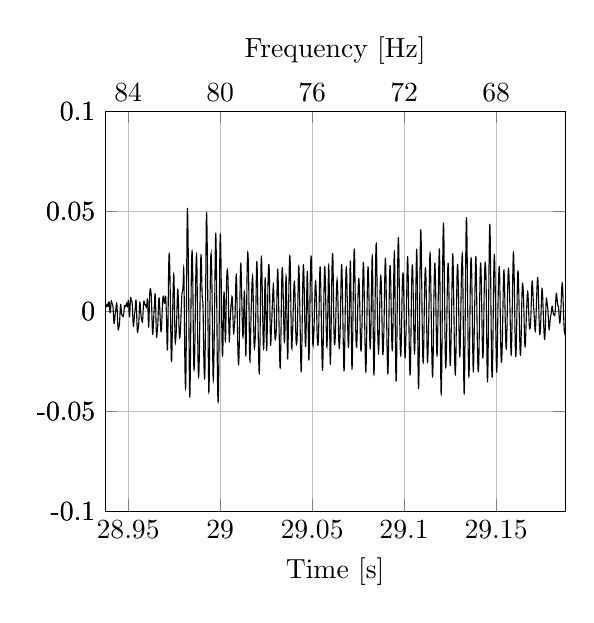
\begin{tikzpicture}


\begin{axis}[%
width=2.3in,
height=2in,
at={(1.011in,0.642in)},
scale only axis,
xmin=28.9375,
xmax=29.1875,
xtick={28.95, 29, 29.05,  29.1, 29.15},
xticklabels={84, 80, 76, 72, 68},
xmajorgrids,
ymin=-0.1,
ymax=0.1,
ymajorgrids,
scaled ticks=false,
ytick={-0.1, -0.05, 0,  0.05, 0.1},
yticklabels={-0.1, -0.05, 0,  0.05, 0.1},
axis x line*=top,
xlabel={Frequency [Hz]},
axis background/.style={fill=white}
]
\end{axis}

\begin{axis}[%
width=2.3in,
height=2in,
at={(1.011in,0.642in)},
scale only axis,
xmin=28.9375,
xmax=29.1875,
xmajorgrids,
ymin=-0.1,
ymax=0.1,
ymajorgrids,
scaled ticks=false,
ytick={-0.1, -0.05, 0,  0.05, 0.1},
yticklabels={-0.1, -0.05, 0,  0.05, 0.1},
xlabel={Time [s]},
axis background/.style={fill=white}
]
\addplot [color=black,solid,forget plot]
table[row sep=crcr]{%
	28.9374791666667	0.00120449066162109\\
	28.9375	0.0013422966003418\\
	28.9375208333333	0.00147902965545654\\
	28.9375416666667	0.00158834457397461\\
	28.9375625	0.00170481204986572\\
	28.9375833333333	0.00182092189788818\\
	28.9376041666667	0.00190639495849609\\
	28.937625	0.00197184085845947\\
	28.9376458333333	0.00206494331359863\\
	28.9376666666667	0.00211882591247559\\
	28.9376875	0.00217843055725098\\
	28.9377083333333	0.00219666957855225\\
	28.9377291666667	0.00223839282989502\\
	28.93775	0.00232481956481934\\
	28.9377708333333	0.00233364105224609\\
	28.9377916666667	0.00235855579376221\\
	28.9378125	0.00237452983856201\\
	28.9378333333333	0.00237023830413818\\
	28.9378541666667	0.00236904621124268\\
	28.937875	0.0023728609085083\\
	28.9378958333333	0.00235486030578613\\
	28.9379166666667	0.00235366821289063\\
	28.9379375	0.00235486030578613\\
	28.9379583333333	0.00233364105224609\\
	28.9379791666667	0.00234019756317139\\
	28.938	0.00231480598449707\\
	28.9380208333333	0.00231778621673584\\
	28.9380416666667	0.00233066082000732\\
	28.9380625	0.00229394435882568\\
	28.9380833333333	0.00233161449432373\\
	28.9381041666667	0.00232195854187012\\
	28.938125	0.00232744216918945\\
	28.9381458333333	0.00236666202545166\\
	28.9381666666667	0.00239074230194092\\
	28.9381875	0.0024111270904541\\
	28.9382083333333	0.00241708755493164\\
	28.9382291666667	0.00250089168548584\\
	28.93825	0.00255060195922852\\
	28.9382708333333	0.00261783599853516\\
	28.9382916666667	0.00265705585479736\\
	28.9383125	0.00270915031433105\\
	28.9383333333333	0.00275206565856934\\
	28.9383541666667	0.00282132625579834\\
	28.938375	0.00291812419891357\\
	28.9383958333333	0.00299406051635742\\
	28.9384166666667	0.00303125381469727\\
	28.9384375	0.00311172008514404\\
	28.9384583333333	0.00321066379547119\\
	28.9384791666667	0.0032811164855957\\
	28.9385	0.00332748889923096\\
	28.9385208333333	0.00336956977844238\\
	28.9385416666667	0.00345480442047119\\
	28.9385625	0.00349807739257813\\
	28.9385833333333	0.00352728366851807\\
	28.9386041666667	0.0035477876663208\\
	28.938625	0.0035707950592041\\
	28.9386458333333	0.00359570980072021\\
	28.9386666666667	0.0036003589630127\\
	28.9386875	0.00357067584991455\\
	28.9387083333333	0.00353062152862549\\
	28.9387291666667	0.00348305702209473\\
	28.93875	0.00348186492919922\\
	28.9387708333333	0.0034555196762085\\
	28.9387916666667	0.00335538387298584\\
	28.9388125	0.00326108932495117\\
	28.9388333333333	0.00318527221679688\\
	28.9388541666667	0.00317442417144775\\
	28.938875	0.00306880474090576\\
	28.9388958333333	0.00293564796447754\\
	28.9389166666667	0.00287473201751709\\
	28.9389375	0.00280296802520752\\
	28.9389583333333	0.00272119045257568\\
	28.9389791666667	0.00266194343566895\\
	28.939	0.00259816646575928\\
	28.9390208333333	0.0025409460067749\\
	28.9390416666667	0.00249350070953369\\
	28.9390625	0.00247383117675781\\
	28.9390833333333	0.00246036052703857\\
	28.9391041666667	0.00245332717895508\\
	28.939125	0.00244832038879395\\
	28.9391458333333	0.00248098373413086\\
	28.9391666666667	0.00252044200897217\\
	28.9391875	0.00253975391387939\\
	28.9392083333333	0.00264823436737061\\
	28.9392291666667	0.00271797180175781\\
	28.93925	0.00281059741973877\\
	28.9392708333333	0.00290811061859131\\
	28.9392916666667	0.00302028656005859\\
	28.9393125	0.00315308570861816\\
	28.9393333333333	0.00329148769378662\\
	28.9393541666667	0.00340831279754639\\
	28.939375	0.00356948375701904\\
	28.9393958333333	0.00372171401977539\\
	28.9394166666667	0.00384736061096191\\
	28.9394375	0.0039832592010498\\
	28.9394583333333	0.00412929058074951\\
	28.9394791666667	0.00424027442932129\\
	28.9395	0.00433218479156494\\
	28.9395208333333	0.00442314147949219\\
	28.9395416666667	0.00449824333190918\\
	28.9395625	0.00455284118652344\\
	28.9395833333333	0.00458669662475586\\
	28.9396041666667	0.0046314001083374\\
	28.939625	0.00459587574005127\\
	28.9396458333333	0.0045621395111084\\
	28.9396666666667	0.00453615188598633\\
	28.9396875	0.0044330358505249\\
	28.9397083333333	0.00432121753692627\\
	28.9397291666667	0.00419533252716064\\
	28.93975	0.00404250621795654\\
	28.9397708333333	0.00387072563171387\\
	28.9397916666667	0.00365662574768066\\
	28.9398125	0.003456711769104\\
	28.9398333333333	0.00322723388671875\\
	28.9398541666667	0.002982497215271\\
	28.939875	0.00272881984710693\\
	28.9398958333333	0.00249087810516357\\
	28.9399166666667	0.00224483013153076\\
	28.9399375	0.00196731090545654\\
	28.9399583333333	0.00170230865478516\\
	28.9399791666667	0.00142776966094971\\
	28.94	0.00115609169006348\\
	28.9400208333333	0.000885367393493652\\
	28.9400416666667	0.000633358955383301\\
	28.9400625	0.000411391258239746\\
	28.9400833333333	0.000180602073669434\\
	28.9401041666667	-8.34465026855469e-06\\
	28.940125	-0.000194072723388672\\
	28.9401458333333	-0.000409603118896484\\
	28.9401666666667	-0.000522017478942871\\
	28.9401875	-0.000576972961425781\\
	28.9402083333333	-0.000643014907836914\\
	28.9402291666667	-0.000677943229675293\\
	28.94025	-0.000661253929138184\\
	28.9402708333333	-0.000652074813842773\\
	28.9402916666667	-0.000607490539550781\\
	28.9403125	-0.000536084175109863\\
	28.9403333333333	-0.000380039215087891\\
	28.9403541666667	-0.000264167785644531\\
	28.940375	-0.00012516975402832\\
	28.9403958333333	1.87158584594727e-05\\
	28.9404166666667	0.000219106674194336\\
	28.9404375	0.000468611717224121\\
	28.9404583333333	0.000717759132385254\\
	28.9404791666667	0.00103902816772461\\
	28.9405	0.00130844116210938\\
	28.9405208333333	0.00157058238983154\\
	28.9405416666667	0.00185871124267578\\
	28.9405625	0.00217807292938232\\
	28.9405833333333	0.00246882438659668\\
	28.9406041666667	0.0027240514755249\\
	28.940625	0.00297737121582031\\
	28.9406458333333	0.00324654579162598\\
	28.9406666666667	0.00350058078765869\\
	28.9406875	0.00375759601593018\\
	28.9407083333333	0.0039670467376709\\
	28.9407291666667	0.00423252582550049\\
	28.94075	0.00441229343414307\\
	28.9407708333333	0.00458657741546631\\
	28.9407916666667	0.00479030609130859\\
	28.9408125	0.00493013858795166\\
	28.9408333333333	0.00502967834472656\\
	28.9408541666667	0.00513112545013428\\
	28.940875	0.00521993637084961\\
	28.9408958333333	0.00522971153259277\\
	28.9409166666667	0.00522172451019287\\
	28.9409375	0.00522911548614502\\
	28.9409583333333	0.00523996353149414\\
	28.9409791666667	0.0052112340927124\\
	28.941	0.00512528419494629\\
	28.9410208333333	0.00503182411193848\\
	28.9410416666667	0.00497424602508545\\
	28.9410625	0.00487077236175537\\
	28.9410833333333	0.00477099418640137\\
	28.9411041666667	0.00464916229248047\\
	28.941125	0.004547119140625\\
	28.9411458333333	0.00443184375762939\\
	28.9411666666667	0.00429177284240723\\
	28.9411875	0.00418353080749512\\
	28.9412083333333	0.00412440299987793\\
	28.9412291666667	0.00401580333709717\\
	28.94125	0.00392568111419678\\
	28.9412708333333	0.00388896465301514\\
	28.9412916666667	0.0037989616394043\\
	28.9413125	0.00372517108917236\\
	28.9413333333333	0.00367295742034912\\
	28.9413541666667	0.00364494323730469\\
	28.941375	0.00362873077392578\\
	28.9413958333333	0.00360417366027832\\
	28.9414166666667	0.00356161594390869\\
	28.9414375	0.00357687473297119\\
	28.9414583333333	0.00352346897125244\\
	28.9414791666667	0.00348567962646484\\
	28.9415	0.00347518920898438\\
	28.9415208333333	0.00347352027893066\\
	28.9415416666667	0.00342643260955811\\
	28.9415625	0.00337326526641846\\
	28.9415833333333	0.00334906578063965\\
	28.9416041666667	0.00328314304351807\\
	28.941625	0.00321304798126221\\
	28.9416458333333	0.00310385227203369\\
	28.9416666666667	0.0030217170715332\\
	28.9416875	0.00289404392242432\\
	28.9417083333333	0.00277328491210938\\
	28.9417291666667	0.00259971618652344\\
	28.94175	0.00243127346038818\\
	28.9417708333333	0.00223422050476074\\
	28.9417916666667	0.00204789638519287\\
	28.9418125	0.00179445743560791\\
	28.9418333333333	0.00156998634338379\\
	28.9418541666667	0.00131797790527344\\
	28.941875	0.00100135803222656\\
	28.9418958333333	0.000730276107788086\\
	28.9419166666667	0.000393033027648926\\
	28.9419375	4.80413436889648e-05\\
	28.9419583333333	-0.000273346900939941\\
	28.9419791666667	-0.000638008117675781\\
	28.942	-0.000986218452453613\\
	28.9420208333333	-0.0013500452041626\\
	28.9420416666667	-0.00172805786132813\\
	28.9420625	-0.00209999084472656\\
	28.9420833333333	-0.00245952606201172\\
	28.9421041666667	-0.00283920764923096\\
	28.942125	-0.00321090221405029\\
	28.9421458333333	-0.00355565547943115\\
	28.9421666666667	-0.00390529632568359\\
	28.9421875	-0.00425815582275391\\
	28.9422083333333	-0.00453579425811768\\
	28.9422291666667	-0.00481522083282471\\
	28.94225	-0.00510096549987793\\
	28.9422708333333	-0.00531721115112305\\
	28.9422916666667	-0.00551402568817139\\
	28.9423125	-0.00571227073669434\\
	28.9423333333333	-0.00587165355682373\\
	28.9423541666667	-0.006011962890625\\
	28.942375	-0.00609862804412842\\
	28.9423958333333	-0.00616216659545898\\
	28.9424166666667	-0.0061640739440918\\
	28.9424375	-0.00617873668670654\\
	28.9424583333333	-0.0061715841293335\\
	28.9424791666667	-0.00609982013702393\\
	28.9425	-0.00601935386657715\\
	28.9425208333333	-0.00593757629394531\\
	28.9425416666667	-0.00584173202514648\\
	28.9425625	-0.00566816329956055\\
	28.9425833333333	-0.00552630424499512\\
	28.9426041666667	-0.00535976886749268\\
	28.942625	-0.00518405437469482\\
	28.9426458333333	-0.00501167774200439\\
	28.9426666666667	-0.00480484962463379\\
	28.9426875	-0.00459206104278564\\
	28.9427083333333	-0.004372239112854\\
	28.9427291666667	-0.00415718555450439\\
	28.94275	-0.00394749641418457\\
	28.9427708333333	-0.00370919704437256\\
	28.9427916666667	-0.00349545478820801\\
	28.9428125	-0.00327563285827637\\
	28.9428333333333	-0.00306379795074463\\
	28.9428541666667	-0.00283503532409668\\
	28.942875	-0.00266897678375244\\
	28.9428958333333	-0.00242698192596436\\
	28.9429166666667	-0.00224006175994873\\
	28.9429375	-0.00203025341033936\\
	28.9429583333333	-0.00185549259185791\\
	28.9429791666667	-0.00171148777008057\\
	28.943	-0.00151622295379639\\
	28.9430208333333	-0.00136935710906982\\
	28.9430416666667	-0.00121152400970459\\
	28.9430625	-0.00106132030487061\\
	28.9430833333333	-0.000919103622436523\\
	28.9431041666667	-0.000782370567321777\\
	28.943125	-0.000638723373413086\\
	28.9431458333333	-0.000498175621032715\\
	28.9431666666667	-0.000345945358276367\\
	28.9431875	-0.000230789184570313\\
	28.9432083333333	-8.38041305541992e-05\\
	28.9432291666667	8.63075256347656e-05\\
	28.94325	0.00023949146270752\\
	28.9432708333333	0.000397205352783203\\
	28.9432916666667	0.000530004501342773\\
	28.9433125	0.000728845596313477\\
	28.9433333333333	0.000880002975463867\\
	28.9433541666667	0.00105178356170654\\
	28.943375	0.00125205516815186\\
	28.9433958333333	0.00144445896148682\\
	28.9434166666667	0.00165307521820068\\
	28.9434375	0.00179791450500488\\
	28.9434583333333	0.00201606750488281\\
	28.9434791666667	0.00223231315612793\\
	28.9435	0.00242531299591064\\
	28.9435208333333	0.00262200832366943\\
	28.9435416666667	0.00280725955963135\\
	28.9435625	0.00299155712127686\\
	28.9435833333333	0.00317680835723877\\
	28.9436041666667	0.00332033634185791\\
	28.943625	0.00349819660186768\\
	28.9436458333333	0.00365996360778809\\
	28.9436666666667	0.00376176834106445\\
	28.9436875	0.0038527250289917\\
	28.9437083333333	0.00394964218139648\\
	28.9437291666667	0.00402390956878662\\
	28.94375	0.00402307510375977\\
	28.9437708333333	0.0040431022644043\\
	28.9437916666667	0.00400960445404053\\
	28.9438125	0.00398123264312744\\
	28.9438333333333	0.00387287139892578\\
	28.9438541666667	0.00376808643341064\\
	28.943875	0.0036466121673584\\
	28.9438958333333	0.00343811511993408\\
	28.9439166666667	0.00322556495666504\\
	28.9439375	0.00299918651580811\\
	28.9439583333333	0.00274956226348877\\
	28.9439791666667	0.00238537788391113\\
	28.944	0.00204110145568848\\
	28.9440208333333	0.00170993804931641\\
	28.9440416666667	0.00127840042114258\\
	28.9440625	0.00086820125579834\\
	28.9440833333333	0.00043022632598877\\
	28.9441041666667	-4.25577163696289e-05\\
	28.944125	-0.000528573989868164\\
	28.9441458333333	-0.000995159149169922\\
	28.9441666666667	-0.00151360034942627\\
	28.9441875	-0.00202596187591553\\
	28.9442083333333	-0.00253725051879883\\
	28.9442291666667	-0.00308370590209961\\
	28.94425	-0.00356650352478027\\
	28.9442708333333	-0.00408291816711426\\
	28.9442916666667	-0.00460159778594971\\
	28.9443125	-0.00507307052612305\\
	28.9443333333333	-0.00550568103790283\\
	28.9443541666667	-0.00596094131469727\\
	28.944375	-0.00639355182647705\\
	28.9443958333333	-0.00678336620330811\\
	28.9444166666667	-0.00715458393096924\\
	28.9444375	-0.00749218463897705\\
	28.9444583333333	-0.00781965255737305\\
	28.9444791666667	-0.00808835029602051\\
	28.9445	-0.00832915306091309\\
	28.9445208333333	-0.00857234001159668\\
	28.9445416666667	-0.0087350606918335\\
	28.9445625	-0.00887703895568848\\
	28.9445833333333	-0.00901639461517334\\
	28.9446041666667	-0.00910532474517822\\
	28.944625	-0.00917530059814453\\
	28.9446458333333	-0.00921499729156494\\
	28.9446666666667	-0.00927221775054932\\
	28.9446875	-0.0092463493347168\\
	28.9447083333333	-0.00926792621612549\\
	28.9447291666667	-0.00922989845275879\\
	28.94475	-0.00919866561889648\\
	28.9447708333333	-0.00914144515991211\\
	28.9447916666667	-0.00907063484191895\\
	28.9448125	-0.00901293754577637\\
	28.9448333333333	-0.00892424583435059\\
	28.9448541666667	-0.00883769989013672\\
	28.944875	-0.00875723361968994\\
	28.9448958333333	-0.00870335102081299\\
	28.9449166666667	-0.0085904598236084\\
	28.9449375	-0.00850820541381836\\
	28.9449583333333	-0.00839269161224365\\
	28.9449791666667	-0.00831711292266846\\
	28.945	-0.0082094669342041\\
	28.9450208333333	-0.00813567638397217\\
	28.9450416666667	-0.00805056095123291\\
	28.9450625	-0.0079272985458374\\
	28.9450833333333	-0.00782966613769531\\
	28.9451041666667	-0.0077434778213501\\
	28.945125	-0.00762271881103516\\
	28.9451458333333	-0.00748217105865479\\
	28.9451666666667	-0.0074012279510498\\
	28.9451875	-0.00725114345550537\\
	28.9452083333333	-0.00711047649383545\\
	28.9452291666667	-0.00694930553436279\\
	28.94525	-0.0067903995513916\\
	28.9452708333333	-0.00657689571380615\\
	28.9452916666667	-0.00638699531555176\\
	28.9453125	-0.00614047050476074\\
	28.9453333333333	-0.00589501857757568\\
	28.9453541666667	-0.00564134120941162\\
	28.945375	-0.00533878803253174\\
	28.9453958333333	-0.0050283670425415\\
	28.9454166666667	-0.0046771764755249\\
	28.9454375	-0.0043487548828125\\
	28.9454583333333	-0.00397193431854248\\
	28.9454791666667	-0.00359225273132324\\
	28.9455	-0.00320053100585938\\
	28.9455208333333	-0.00277113914489746\\
	28.9455416666667	-0.00234317779541016\\
	28.9455625	-0.00193297863006592\\
	28.9455833333333	-0.00148999691009521\\
	28.9456041666667	-0.0010521411895752\\
	28.945625	-0.000657558441162109\\
	28.9456458333333	-0.000228643417358398\\
	28.9456666666667	0.000164389610290527\\
	28.9456875	0.000571966171264648\\
	28.9457083333333	0.000959157943725586\\
	28.9457291666667	0.0012742280960083\\
	28.94575	0.00164806842803955\\
	28.9457708333333	0.00197863578796387\\
	28.9457916666667	0.00224733352661133\\
	28.9458125	0.00248706340789795\\
	28.9458333333333	0.00269651412963867\\
	28.9458541666667	0.00291526317596436\\
	28.945875	0.00307631492614746\\
	28.9458958333333	0.00319766998291016\\
	28.9459166666667	0.00328361988067627\\
	28.9459375	0.00333547592163086\\
	28.9459583333333	0.0033566951751709\\
	28.9459791666667	0.00334405899047852\\
	28.946	0.00330209732055664\\
	28.9460208333333	0.00322556495666504\\
	28.9460416666667	0.00311374664306641\\
	28.9460625	0.00297248363494873\\
	28.9460833333333	0.00281548500061035\\
	28.9461041666667	0.00264823436737061\\
	28.946125	0.00243580341339111\\
	28.9461458333333	0.00223219394683838\\
	28.9461666666667	0.00200450420379639\\
	28.9461875	0.00174605846405029\\
	28.9462083333333	0.00149452686309814\\
	28.9462291666667	0.00123834609985352\\
	28.94625	0.000975608825683594\\
	28.9462708333333	0.000711798667907715\\
	28.9462916666667	0.000437259674072266\\
	28.9463125	0.000186920166015625\\
	28.9463333333333	-4.62532043457031e-05\\
	28.9463541666667	-0.000296592712402344\\
	28.946375	-0.000509381294250488\\
	28.9463958333333	-0.000693798065185547\\
	28.9464166666667	-0.000870347023010254\\
	28.9464375	-0.00106263160705566\\
	28.9464583333333	-0.00124084949493408\\
	28.9464791666667	-0.00135302543640137\\
	28.9465	-0.00150108337402344\\
	28.9465208333333	-0.00159585475921631\\
	28.9465416666667	-0.00174951553344727\\
	28.9465625	-0.00178027153015137\\
	28.9465833333333	-0.00185716152191162\\
	28.9466041666667	-0.00190210342407227\\
	28.946625	-0.00194311141967773\\
	28.9466458333333	-0.00195682048797607\\
	28.9466666666667	-0.00200092792510986\\
	28.9466875	-0.00200068950653076\\
	28.9467083333333	-0.00199317932128906\\
	28.9467291666667	-0.00199985504150391\\
	28.94675	-0.00198268890380859\\
	28.9467708333333	-0.00201892852783203\\
	28.9467916666667	-0.00195181369781494\\
	28.9468125	-0.00197136402130127\\
	28.9468333333333	-0.00197088718414307\\
	28.9468541666667	-0.00195300579071045\\
	28.946875	-0.0019221305847168\\
	28.9468958333333	-0.00193166732788086\\
	28.9469166666667	-0.00193977355957031\\
	28.9469375	-0.00197398662567139\\
	28.9469583333333	-0.00198137760162354\\
	28.9469791666667	-0.00202929973602295\\
	28.947	-0.00204813480377197\\
	28.9470208333333	-0.00205314159393311\\
	28.9470416666667	-0.0021357536315918\\
	28.9470625	-0.00214993953704834\\
	28.9470833333333	-0.0022275447845459\\
	28.9471041666667	-0.00226342678070068\\
	28.947125	-0.0023338794708252\\
	28.9471458333333	-0.0023953914642334\\
	28.9471666666667	-0.00243794918060303\\
	28.9471875	-0.00251471996307373\\
	28.9472083333333	-0.00256145000457764\\
	28.9472291666667	-0.00262069702148438\\
	28.94725	-0.00264477729797363\\
	28.9472708333333	-0.00268018245697021\\
	28.9472916666667	-0.00271868705749512\\
	28.9473125	-0.00275373458862305\\
	28.9473333333333	-0.0027240514755249\\
	28.9473541666667	-0.00271487236022949\\
	28.947375	-0.00269734859466553\\
	28.9473958333333	-0.00266361236572266\\
	28.9474166666667	-0.00259816646575928\\
	28.9474375	-0.00254809856414795\\
	28.9474583333333	-0.0024724006652832\\
	28.9474791666667	-0.00236475467681885\\
	28.9475	-0.00222373008728027\\
	28.9475208333333	-0.00209498405456543\\
	28.9475416666667	-0.00199651718139648\\
	28.9475625	-0.00181496143341064\\
	28.9475833333333	-0.00161874294281006\\
	28.9476041666667	-0.00142979621887207\\
	28.947625	-0.00125586986541748\\
	28.9476458333333	-0.00103628635406494\\
	28.9476666666667	-0.00085151195526123\\
	28.9476875	-0.000629663467407227\\
	28.9477083333333	-0.000427961349487305\\
	28.9477291666667	-0.000189900398254395\\
	28.94775	2.43186950683594e-05\\
	28.9477708333333	0.000212907791137695\\
	28.9477916666667	0.000438451766967773\\
	28.9478125	0.000701308250427246\\
	28.9478333333333	0.000888824462890625\\
	28.9478541666667	0.00107264518737793\\
	28.947875	0.00127303600311279\\
	28.9478958333333	0.00148415565490723\\
	28.9479166666667	0.00163650512695313\\
	28.9479375	0.00178205966949463\\
	28.9479583333333	0.0019611120223999\\
	28.9479791666667	0.00208234786987305\\
	28.948	0.0022122859954834\\
	28.9480208333333	0.00233030319213867\\
	28.9480416666667	0.00245213508605957\\
	28.9480625	0.00254130363464355\\
	28.9480833333333	0.00261390209197998\\
	28.9481041666667	0.00266730785369873\\
	28.948125	0.002768874168396\\
	28.9481458333333	0.00282394886016846\\
	28.9481666666667	0.00283098220825195\\
	28.9481875	0.00286483764648438\\
	28.9482083333333	0.00290322303771973\\
	28.9482291666667	0.00289678573608398\\
	28.94825	0.0028834342956543\\
	28.9482708333333	0.00288903713226318\\
	28.9482916666667	0.00288474559783936\\
	28.9483125	0.00286269187927246\\
	28.9483333333333	0.00282883644104004\\
	28.9483541666667	0.00279414653778076\\
	28.948375	0.00276303291320801\\
	28.9483958333333	0.00272870063781738\\
	28.9484166666667	0.00271797180175781\\
	28.9484375	0.00267577171325684\\
	28.9484583333333	0.00263571739196777\\
	28.9484791666667	0.00257432460784912\\
	28.9485	0.00260186195373535\\
	28.9485208333333	0.00261199474334717\\
	28.9485416666667	0.0025259256362915\\
	28.9485625	0.00253629684448242\\
	28.9485833333333	0.00254309177398682\\
	28.9486041666667	0.00254881381988525\\
	28.948625	0.00251924991607666\\
	28.9486458333333	0.00258731842041016\\
	28.9486666666667	0.0026010274887085\\
	28.9486875	0.00260651111602783\\
	28.9487083333333	0.00261986255645752\\
	28.9487291666667	0.00269746780395508\\
	28.94875	0.00275719165802002\\
	28.9487708333333	0.00278258323669434\\
	28.9487916666667	0.00282752513885498\\
	28.9488125	0.00287473201751709\\
	28.9488333333333	0.00293600559234619\\
	28.9488541666667	0.00301527976989746\\
	28.948875	0.0030893087387085\\
	28.9488958333333	0.00317025184631348\\
	28.9489166666667	0.00324559211730957\\
	28.9489375	0.00328946113586426\\
	28.9489583333333	0.00333797931671143\\
	28.9489791666667	0.00340175628662109\\
	28.949	0.00345754623413086\\
	28.9490208333333	0.00350940227508545\\
	28.9490416666667	0.00359416007995605\\
	28.9490625	0.00362908840179443\\
	28.9490833333333	0.00361824035644531\\
	28.9491041666667	0.0036015510559082\\
	28.949125	0.00365960597991943\\
	28.9491458333333	0.00370883941650391\\
	28.9491666666667	0.00361740589141846\\
	28.9491875	0.00354647636413574\\
	28.9492083333333	0.00355947017669678\\
	28.9492291666667	0.00348484516143799\\
	28.94925	0.00344514846801758\\
	28.9492708333333	0.00336253643035889\\
	28.9492916666667	0.00326979160308838\\
	28.9493125	0.00314474105834961\\
	28.9493333333333	0.00303030014038086\\
	28.9493541666667	0.00299572944641113\\
	28.949375	0.00288474559783936\\
	28.9493958333333	0.00273466110229492\\
	28.9494166666667	0.00265610218048096\\
	28.9494375	0.00257062911987305\\
	28.9494583333333	0.00245749950408936\\
	28.9494791666667	0.00238919258117676\\
	28.9495	0.00232481956481934\\
	28.9495208333333	0.00229990482330322\\
	28.9495416666667	0.00223338603973389\\
	28.9495625	0.002205491065979\\
	28.9495833333333	0.00222384929656982\\
	28.9496041666667	0.00224018096923828\\
	28.949625	0.00226807594299316\\
	28.9496458333333	0.002349853515625\\
	28.9496666666667	0.00245094299316406\\
	28.9496875	0.00250637531280518\\
	28.9497083333333	0.0025869607925415\\
	28.9497291666667	0.00275886058807373\\
	28.94975	0.00294363498687744\\
	28.9497708333333	0.00306534767150879\\
	28.9497916666667	0.00320351123809814\\
	28.9498125	0.00345981121063232\\
	28.9498333333333	0.00364840030670166\\
	28.9498541666667	0.00382018089294434\\
	28.949875	0.00399625301361084\\
	28.9498958333333	0.00420570373535156\\
	28.9499166666667	0.00439226627349854\\
	28.9499375	0.00453698635101318\\
	28.9499583333333	0.0047307014465332\\
	28.9499791666667	0.00490379333496094\\
	28.95	0.00499629974365234\\
	28.9500208333333	0.00507068634033203\\
	28.9500416666667	0.00517380237579346\\
	28.9500625	0.00527513027191162\\
	28.9500833333333	0.00526750087738037\\
	28.9501041666667	0.00522792339324951\\
	28.950125	0.00524055957794189\\
	28.9501458333333	0.00517702102661133\\
	28.9501666666667	0.00502884387969971\\
	28.9501875	0.00488781929016113\\
	28.9502083333333	0.00475656986236572\\
	28.9502291666667	0.00458204746246338\\
	28.95025	0.00433135032653809\\
	28.9502708333333	0.00405228137969971\\
	28.9502916666667	0.00383269786834717\\
	28.9503125	0.00350522994995117\\
	28.9503333333333	0.00316107273101807\\
	28.9503541666667	0.00278890132904053\\
	28.950375	0.00247848033905029\\
	28.9503958333333	0.00213134288787842\\
	28.9504166666667	0.0016934871673584\\
	28.9504375	0.00128757953643799\\
	28.9504583333333	0.000902414321899414\\
	28.9504791666667	0.000477790832519531\\
	28.9505	3.38554382324219e-05\\
	28.9505208333333	-0.000324130058288574\\
	28.9505416666667	-0.000696778297424316\\
	28.9505625	-0.00110518932342529\\
	28.9505833333333	-0.00148618221282959\\
	28.9506041666667	-0.0017240047454834\\
	28.950625	-0.00196230411529541\\
	28.9506458333333	-0.00223922729492188\\
	28.9506666666667	-0.00240206718444824\\
	28.9506875	-0.00247740745544434\\
	28.9507083333333	-0.00260722637176514\\
	28.9507291666667	-0.00270664691925049\\
	28.95075	-0.00269615650177002\\
	28.9507708333333	-0.00262069702148438\\
	28.9507916666667	-0.00257313251495361\\
	28.9508125	-0.0025097131729126\\
	28.9508333333333	-0.00235104560852051\\
	28.9508541666667	-0.00208103656768799\\
	28.950875	-0.00179779529571533\\
	28.9508958333333	-0.00150954723358154\\
	28.9509166666667	-0.00117194652557373\\
	28.9509375	-0.000782370567321777\\
	28.9509583333333	-0.00044858455657959\\
	28.9509791666667	-8.34465026855469e-05\\
	28.951	0.000378012657165527\\
	28.9510208333333	0.000835776329040527\\
	28.9510416666667	0.00127923488616943\\
	28.9510625	0.00171661376953125\\
	28.9510833333333	0.00211620330810547\\
	28.9511041666667	0.00249087810516357\\
	28.951125	0.00293815135955811\\
	28.9511458333333	0.00336539745330811\\
	28.9511666666667	0.00378096103668213\\
	28.9511875	0.00420570373535156\\
	28.9512083333333	0.004599928855896\\
	28.9512291666667	0.00494003295898438\\
	28.95125	0.00526010990142822\\
	28.9512708333333	0.00555706024169922\\
	28.9512916666667	0.00581920146942139\\
	28.9513125	0.00606405735015869\\
	28.9513333333333	0.0062861442565918\\
	28.9513541666667	0.00645327568054199\\
	28.951375	0.00657689571380615\\
	28.9513958333333	0.00669670104980469\\
	28.9514166666667	0.00680875778198242\\
	28.9514375	0.00682854652404785\\
	28.9514583333333	0.00684773921966553\\
	28.9514791666667	0.00681555271148682\\
	28.9515	0.00680291652679443\\
	28.9515208333333	0.00669407844543457\\
	28.9515416666667	0.00658977031707764\\
	28.9515625	0.00653398036956787\\
	28.9515833333333	0.00641906261444092\\
	28.9516041666667	0.00633645057678223\\
	28.951625	0.0062251091003418\\
	28.9516458333333	0.00611782073974609\\
	28.9516666666667	0.00599849224090576\\
	28.9516875	0.00585758686065674\\
	28.9517083333333	0.00576698780059814\\
	28.9517291666667	0.00570058822631836\\
	28.95175	0.00557601451873779\\
	28.9517708333333	0.00548863410949707\\
	28.9517916666667	0.00545024871826172\\
	28.9518125	0.00538110733032227\\
	28.9518333333333	0.0052955150604248\\
	28.9518541666667	0.0052649974822998\\
	28.951875	0.00523805618286133\\
	28.9518958333333	0.00520634651184082\\
	28.9519166666667	0.0051729679107666\\
	28.9519375	0.00515663623809814\\
	28.9519583333333	0.00512909889221191\\
	28.9519791666667	0.00505387783050537\\
	28.952	0.00503396987915039\\
	28.9520208333333	0.0050126314163208\\
	28.9520416666667	0.00497937202453613\\
	28.9520625	0.00488507747650146\\
	28.9520833333333	0.00477564334869385\\
	28.9521041666667	0.00469386577606201\\
	28.952125	0.00460553169250488\\
	28.9521458333333	0.00447690486907959\\
	28.9521666666667	0.00430679321289063\\
	28.9521875	0.00413095951080322\\
	28.9522083333333	0.00396382808685303\\
	28.9522291666667	0.00372219085693359\\
	28.95225	0.00348925590515137\\
	28.9522708333333	0.00323283672332764\\
	28.9522916666667	0.00292778015136719\\
	28.9523125	0.00257265567779541\\
	28.9523333333333	0.00225222110748291\\
	28.9523541666667	0.00188350677490234\\
	28.952375	0.00146079063415527\\
	28.9523958333333	0.00111985206604004\\
	28.9524166666667	0.000669598579406738\\
	28.9524375	0.000219464302062988\\
	28.9524583333333	-0.000203490257263184\\
	28.9524791666667	-0.000688910484313965\\
	28.9525	-0.00115406513214111\\
	28.9525208333333	-0.00164473056793213\\
	28.9525416666667	-0.00214004516601563\\
	28.9525625	-0.00266695022583008\\
	28.9525833333333	-0.00313663482666016\\
	28.9526041666667	-0.00356113910675049\\
	28.952625	-0.00401782989501953\\
	28.9526458333333	-0.00445592403411865\\
	28.9526666666667	-0.00490152835845947\\
	28.9526875	-0.00530540943145752\\
	28.9527083333333	-0.00565338134765625\\
	28.9527291666667	-0.0059959888458252\\
	28.95275	-0.00635015964508057\\
	28.9527708333333	-0.00661516189575195\\
	28.9527916666667	-0.00686180591583252\\
	28.9528125	-0.00709497928619385\\
	28.9528333333333	-0.00728070735931396\\
	28.9528541666667	-0.00741219520568848\\
	28.952875	-0.00749480724334717\\
	28.9528958333333	-0.00756931304931641\\
	28.9529166666667	-0.00758779048919678\\
	28.9529375	-0.00757312774658203\\
	28.9529583333333	-0.00751519203186035\\
	28.9529791666667	-0.00745391845703125\\
	28.953	-0.00731074810028076\\
	28.9530208333333	-0.00720894336700439\\
	28.9530416666667	-0.00704288482666016\\
	28.9530625	-0.00687050819396973\\
	28.9530833333333	-0.00668728351593018\\
	28.9531041666667	-0.00647926330566406\\
	28.953125	-0.00625467300415039\\
	28.9531458333333	-0.00600981712341309\\
	28.9531666666667	-0.00573980808258057\\
	28.9531875	-0.00549042224884033\\
	28.9532083333333	-0.0052182674407959\\
	28.9532291666667	-0.00494956970214844\\
	28.95325	-0.00468552112579346\\
	28.9532708333333	-0.00440812110900879\\
	28.9532916666667	-0.00417304039001465\\
	28.9533125	-0.00392496585845947\\
	28.9533333333333	-0.00367546081542969\\
	28.9533541666667	-0.00341963768005371\\
	28.953375	-0.00317132472991943\\
	28.9533958333333	-0.00293517112731934\\
	28.9534166666667	-0.00268399715423584\\
	28.9534375	-0.00247335433959961\\
	28.9534583333333	-0.00228261947631836\\
	28.9534791666667	-0.00204145908355713\\
	28.9535	-0.00187921524047852\\
	28.9535208333333	-0.00170278549194336\\
	28.9535416666667	-0.00151956081390381\\
	28.9535625	-0.00134849548339844\\
	28.9535833333333	-0.00116229057312012\\
	28.9536041666667	-0.00100100040435791\\
	28.953625	-0.000794291496276855\\
	28.9536458333333	-0.000609517097473145\\
	28.9536666666667	-0.000457167625427246\\
	28.9536875	-0.000290870666503906\\
	28.9537083333333	-6.79492950439453e-05\\
	28.9537291666667	0.000105500221252441\\
	28.95375	0.000274181365966797\\
	28.9537708333333	0.000500321388244629\\
	28.9537916666667	0.000700950622558594\\
	28.9538125	0.000948309898376465\\
	28.9538333333333	0.00116086006164551\\
	28.9538541666667	0.0013805627822876\\
	28.953875	0.00164890289306641\\
	28.9538958333333	0.00190436840057373\\
	28.9539166666667	0.00211906433105469\\
	28.9539375	0.00242495536804199\\
	28.9539583333333	0.00268375873565674\\
	28.9539791666667	0.00295066833496094\\
	28.954	0.00319314002990723\\
	28.9540208333333	0.00344312191009521\\
	28.9540416666667	0.00373101234436035\\
	28.9540625	0.00397837162017822\\
	28.9540833333333	0.00425004959106445\\
	28.9541041666667	0.00446522235870361\\
	28.954125	0.0046539306640625\\
	28.9541458333333	0.0048515796661377\\
	28.9541666666667	0.00503635406494141\\
	28.9541875	0.00519454479217529\\
	28.9542083333333	0.00532019138336182\\
	28.9542291666667	0.00537395477294922\\
	28.95425	0.00546491146087646\\
	28.9542708333333	0.00549256801605225\\
	28.9542916666667	0.00544416904449463\\
	28.9543125	0.00538980960845947\\
	28.9543333333333	0.00531816482543945\\
	28.9543541666667	0.00517880916595459\\
	28.954375	0.0049821138381958\\
	28.9543958333333	0.00475597381591797\\
	28.9544166666667	0.00447738170623779\\
	28.9544375	0.00416076183319092\\
	28.9544583333333	0.00379776954650879\\
	28.9544791666667	0.00340592861175537\\
	28.9545	0.00294911861419678\\
	28.9545208333333	0.00252604484558105\\
	28.9545416666667	0.00204122066497803\\
	28.9545625	0.00148046016693115\\
	28.9545833333333	0.000900387763977051\\
	28.9546041666667	0.000314235687255859\\
	28.954625	-0.000279426574707031\\
	28.9546458333333	-0.000893354415893555\\
	28.9546666666667	-0.00152122974395752\\
	28.9546875	-0.00219964981079102\\
	28.9547083333333	-0.00283873081207275\\
	28.9547291666667	-0.0034942626953125\\
	28.95475	-0.00412964820861816\\
	28.9547708333333	-0.00474798679351807\\
	28.9547916666667	-0.00536942481994629\\
	28.9548125	-0.00594055652618408\\
	28.9548333333333	-0.00648868083953857\\
	28.9548541666667	-0.00704109668731689\\
	28.954875	-0.00754189491271973\\
	28.9548958333333	-0.00797832012176514\\
	28.9549166666667	-0.00843691825866699\\
	28.9549375	-0.00882446765899658\\
	28.9549583333333	-0.00917530059814453\\
	28.9549791666667	-0.00946581363677979\\
	28.955	-0.00973606109619141\\
	28.9550208333333	-0.00999271869659424\\
	28.9550416666667	-0.0101704597473145\\
	28.9550625	-0.0103230476379395\\
	28.9550833333333	-0.0104254484176636\\
	28.9551041666667	-0.0105032920837402\\
	28.955125	-0.0105493068695068\\
	28.9551458333333	-0.0105750560760498\\
	28.9551666666667	-0.0105768442153931\\
	28.9551875	-0.0105404853820801\\
	28.9552083333333	-0.0104724168777466\\
	28.9552291666667	-0.0103836059570313\\
	28.95525	-0.010285496711731\\
	28.9552708333333	-0.0101571083068848\\
	28.9552916666667	-0.0100215673446655\\
	28.9553125	-0.00990748405456543\\
	28.9553333333333	-0.00978660583496094\\
	28.9553541666667	-0.00964224338531494\\
	28.955375	-0.0095217227935791\\
	28.9553958333333	-0.00938808917999268\\
	28.9554166666667	-0.0092320442199707\\
	28.9554375	-0.00913023948669434\\
	28.9554583333333	-0.00894427299499512\\
	28.9554791666667	-0.00882101058959961\\
	28.9555	-0.0086979866027832\\
	28.9555208333333	-0.00857293605804443\\
	28.9555416666667	-0.00847065448760986\\
	28.9555625	-0.00832951068878174\\
	28.9555833333333	-0.0082094669342041\\
	28.9556041666667	-0.00808465480804443\\
	28.955625	-0.00793445110321045\\
	28.9556458333333	-0.00778770446777344\\
	28.9556666666667	-0.0076291561126709\\
	28.9556875	-0.00744998455047607\\
	28.9557083333333	-0.00727570056915283\\
	28.9557291666667	-0.00702822208404541\\
	28.95575	-0.00678634643554688\\
	28.9557708333333	-0.00655519962310791\\
	28.9557916666667	-0.00625503063201904\\
	28.9558125	-0.00593018531799316\\
	28.9558333333333	-0.00559592247009277\\
	28.9558541666667	-0.00524747371673584\\
	28.955875	-0.00481438636779785\\
	28.9558958333333	-0.0044022798538208\\
	28.9559166666667	-0.0039752721786499\\
	28.9559375	-0.00349390506744385\\
	28.9559583333333	-0.00299704074859619\\
	28.9559791666667	-0.00252139568328857\\
	28.956	-0.00204360485076904\\
	28.9560208333333	-0.00151491165161133\\
	28.9560416666667	-0.00101673603057861\\
	28.9560625	-0.000505208969116211\\
	28.9560833333333	-7.15255737304688e-07\\
	28.9561041666667	0.000502347946166992\\
	28.956125	0.000982284545898438\\
	28.9561458333333	0.00147163867950439\\
	28.9561666666667	0.00189208984375\\
	28.9561875	0.00230145454406738\\
	28.9562083333333	0.00271952152252197\\
	28.9562291666667	0.00310266017913818\\
	28.95625	0.00342249870300293\\
	28.9562708333333	0.00370335578918457\\
	28.9562916666667	0.00393462181091309\\
	28.9563125	0.00415194034576416\\
	28.9563333333333	0.00431013107299805\\
	28.9563541666667	0.00444197654724121\\
	28.956375	0.00454044342041016\\
	28.9563958333333	0.00458753108978271\\
	28.9564166666667	0.0045846700668335\\
	28.9564375	0.00454378128051758\\
	28.9564583333333	0.00447869300842285\\
	28.9564791666667	0.00437462329864502\\
	28.9565	0.00427126884460449\\
	28.9565208333333	0.00410723686218262\\
	28.9565416666667	0.00391364097595215\\
	28.9565625	0.00366950035095215\\
	28.9565833333333	0.00344395637512207\\
	28.9566041666667	0.00315606594085693\\
	28.956625	0.0028681755065918\\
	28.9566458333333	0.00257217884063721\\
	28.9566666666667	0.00225400924682617\\
	28.9566875	0.00198066234588623\\
	28.9567083333333	0.00165057182312012\\
	28.9567291666667	0.00133812427520752\\
	28.95675	0.00105643272399902\\
	28.9567708333333	0.000751376152038574\\
	28.9567916666667	0.000424861907958984\\
	28.9568125	0.000171065330505371\\
	28.9568333333333	-9.0479850769043e-05\\
	28.9568541666667	-0.000412583351135254\\
	28.956875	-0.000677227973937988\\
	28.9568958333333	-0.000899434089660645\\
	28.9569166666667	-0.00112056732177734\\
	28.9569375	-0.00137567520141602\\
	28.9569583333333	-0.00157546997070313\\
	28.9569791666667	-0.00175034999847412\\
	28.957	-0.00192892551422119\\
	28.9570208333333	-0.00210666656494141\\
	28.9570416666667	-0.00226378440856934\\
	28.9570625	-0.00239062309265137\\
	28.9570833333333	-0.00253975391387939\\
	28.9571041666667	-0.00269770622253418\\
	28.957125	-0.00281667709350586\\
	28.9571458333333	-0.0028921365737915\\
	28.9571666666667	-0.00301814079284668\\
	28.9571875	-0.00316214561462402\\
	28.9572083333333	-0.00325405597686768\\
	28.9572291666667	-0.00332438945770264\\
	28.95725	-0.00347423553466797\\
	28.9572708333333	-0.00358736515045166\\
	28.9572916666667	-0.00364816188812256\\
	28.9573125	-0.00376880168914795\\
	28.9573333333333	-0.00388860702514648\\
	28.9573541666667	-0.00401592254638672\\
	28.957375	-0.00411760807037354\\
	28.9573958333333	-0.00422906875610352\\
	28.9574166666667	-0.00434303283691406\\
	28.9574375	-0.00446224212646484\\
	28.9574583333333	-0.00459122657775879\\
	28.9574791666667	-0.00470340251922607\\
	28.9575	-0.00483143329620361\\
	28.9575208333333	-0.00491082668304443\\
	28.9575416666667	-0.00500977039337158\\
	28.9575625	-0.00514519214630127\\
	28.9575833333333	-0.0052182674407959\\
	28.9576041666667	-0.00528013706207275\\
	28.957625	-0.00533974170684814\\
	28.9576458333333	-0.00541150569915771\\
	28.9576666666667	-0.0054318904876709\\
	28.9576875	-0.00544106960296631\\
	28.9577083333333	-0.00546121597290039\\
	28.9577291666667	-0.00540852546691895\\
	28.95775	-0.00538194179534912\\
	28.9577708333333	-0.0053030252456665\\
	28.9577916666667	-0.00520288944244385\\
	28.9578125	-0.00511598587036133\\
	28.9578333333333	-0.00496828556060791\\
	28.9578541666667	-0.00479567050933838\\
	28.957875	-0.00462913513183594\\
	28.9578958333333	-0.00439846515655518\\
	28.9579166666667	-0.00417149066925049\\
	28.9579375	-0.00386989116668701\\
	28.9579583333333	-0.00359725952148438\\
	28.9579791666667	-0.00328981876373291\\
	28.958	-0.0029522180557251\\
	28.9580208333333	-0.00262069702148438\\
	28.9580416666667	-0.00224769115447998\\
	28.9580625	-0.00188589096069336\\
	28.9580833333333	-0.0014883279800415\\
	28.9581041666667	-0.00112724304199219\\
	28.958125	-0.000753998756408691\\
	28.9581458333333	-0.000306248664855957\\
	28.9581666666667	8.85725021362305e-05\\
	28.9581875	0.000467658042907715\\
	28.9582083333333	0.000868678092956543\\
	28.9582291666667	0.00126349925994873\\
	28.95825	0.00159382820129395\\
	28.9582708333333	0.00193023681640625\\
	28.9582916666667	0.0022960901260376\\
	28.9583125	0.00263822078704834\\
	28.9583333333333	0.00293898582458496\\
	28.9583541666667	0.00319647789001465\\
	28.958375	0.00343501567840576\\
	28.9583958333333	0.00368666648864746\\
	28.9584166666667	0.0039290189743042\\
	28.9584375	0.00411438941955566\\
	28.9584583333333	0.00428915023803711\\
	28.9584791666667	0.00444447994232178\\
	28.9585	0.00455582141876221\\
	28.9585208333333	0.00466132164001465\\
	28.9585416666667	0.00477266311645508\\
	28.9585625	0.00482368469238281\\
	28.9585833333333	0.00485706329345703\\
	28.9586041666667	0.00491297245025635\\
	28.958625	0.00495719909667969\\
	28.9586458333333	0.00490915775299072\\
	28.9586666666667	0.00486946105957031\\
	28.9586875	0.00485026836395264\\
	28.9587083333333	0.00480246543884277\\
	28.9587291666667	0.00474405288696289\\
	28.95875	0.00468635559082031\\
	28.9587708333333	0.00462841987609863\\
	28.9587916666667	0.00449824333190918\\
	28.9588125	0.00438845157623291\\
	28.9588333333333	0.00435793399810791\\
	28.9588541666667	0.00428080558776855\\
	28.958875	0.0041424036026001\\
	28.9588958333333	0.00405645370483398\\
	28.9589166666667	0.00400471687316895\\
	28.9589375	0.00390815734863281\\
	28.9589583333333	0.00382733345031738\\
	28.9589791666667	0.00376176834106445\\
	28.959	0.00368845462799072\\
	28.9590208333333	0.00362837314605713\\
	28.9590416666667	0.00353908538818359\\
	28.9590625	0.00352597236633301\\
	28.9590833333333	0.00348150730133057\\
	28.9591041666667	0.00338888168334961\\
	28.959125	0.00334370136260986\\
	28.9591458333333	0.00332820415496826\\
	28.9591666666667	0.00326156616210938\\
	28.9591875	0.00322854518890381\\
	28.9592083333333	0.00319218635559082\\
	28.9592291666667	0.00316357612609863\\
	28.95925	0.0031430721282959\\
	28.9592708333333	0.00309181213378906\\
	28.9592916666667	0.00307798385620117\\
	28.9593125	0.00307083129882813\\
	28.9593333333333	0.00307929515838623\\
	28.9593541666667	0.00302028656005859\\
	28.959375	0.00298082828521729\\
	28.9593958333333	0.00300610065460205\\
	28.9594166666667	0.00300836563110352\\
	28.9594375	0.00296783447265625\\
	28.9594583333333	0.00297856330871582\\
	28.9594791666667	0.00301039218902588\\
	28.9595	0.00296151638031006\\
	28.9595208333333	0.00294613838195801\\
	28.9595416666667	0.00297081470489502\\
	28.9595625	0.00295579433441162\\
	28.9595833333333	0.00286734104156494\\
	28.9596041666667	0.0028759241104126\\
	28.959625	0.00288176536560059\\
	28.9596458333333	0.00281000137329102\\
	28.9596666666667	0.00275087356567383\\
	28.9596875	0.00270700454711914\\
	28.9597083333333	0.00270462036132813\\
	28.9597291666667	0.0026094913482666\\
	28.95975	0.00251424312591553\\
	28.9597708333333	0.00248515605926514\\
	28.9597916666667	0.00244176387786865\\
	28.9598125	0.00230515003204346\\
	28.9598333333333	0.00226759910583496\\
	28.9598541666667	0.00228989124298096\\
	28.959875	0.00221312046051025\\
	28.9598958333333	0.00210249423980713\\
	28.9599166666667	0.00208449363708496\\
	28.9599375	0.0022047758102417\\
	28.9599583333333	0.00214290618896484\\
	28.9599791666667	0.00208067893981934\\
	28.96	0.00213503837585449\\
	28.9600208333333	0.00225937366485596\\
	28.9600416666667	0.00232577323913574\\
	28.9600625	0.00237166881561279\\
	28.9600833333333	0.00248968601226807\\
	28.9601041666667	0.00265204906463623\\
	28.960125	0.00277423858642578\\
	28.9601458333333	0.00292432308197021\\
	28.9601666666667	0.00315630435943604\\
	28.9601875	0.00336587429046631\\
	28.9602083333333	0.00355863571166992\\
	28.9602291666667	0.00375306606292725\\
	28.96025	0.0039900541305542\\
	28.9602708333333	0.00423324108123779\\
	28.9602916666667	0.00445401668548584\\
	28.9603125	0.00469350814819336\\
	28.9603333333333	0.00496053695678711\\
	28.9603541666667	0.00517582893371582\\
	28.960375	0.00533473491668701\\
	28.9603958333333	0.00551259517669678\\
	28.9604166666667	0.00574064254760742\\
	28.9604375	0.0058741569519043\\
	28.9604583333333	0.00594353675842285\\
	28.9604791666667	0.0060044527053833\\
	28.9605	0.00608706474304199\\
	28.9605208333333	0.00607001781463623\\
	28.9605416666667	0.00602066516876221\\
	28.9605625	0.00594222545623779\\
	28.9605833333333	0.00582301616668701\\
	28.9606041666667	0.00564396381378174\\
	28.960625	0.00539326667785645\\
	28.9606458333333	0.00517582893371582\\
	28.9606666666667	0.00482869148254395\\
	28.9606875	0.0044102668762207\\
	28.9607083333333	0.00404214859008789\\
	28.9607291666667	0.00359189510345459\\
	28.96075	0.00300586223602295\\
	28.9607708333333	0.00237274169921875\\
	28.9607916666667	0.00178325176239014\\
	28.9608125	0.00113105773925781\\
	28.9608333333333	0.000365495681762695\\
	28.9608541666667	-0.000380992889404297\\
	28.960875	-0.00107312202453613\\
	28.9608958333333	-0.0018237829208374\\
	28.9609166666667	-0.00260269641876221\\
	28.9609375	-0.00324511528015137\\
	28.9609583333333	-0.00386106967926025\\
	28.9609791666667	-0.0044701099395752\\
	28.961	-0.00507402420043945\\
	28.9610208333333	-0.0055617094039917\\
	28.9610416666667	-0.00603234767913818\\
	28.9610625	-0.006522536277771\\
	28.9610833333333	-0.00686502456665039\\
	28.9611041666667	-0.00710511207580566\\
	28.961125	-0.00736713409423828\\
	28.9611458333333	-0.00761115550994873\\
	28.9611666666667	-0.00773429870605469\\
	28.9611875	-0.00770509243011475\\
	28.9612083333333	-0.00755345821380615\\
	28.9612291666667	-0.00736665725708008\\
	28.96125	-0.00708878040313721\\
	28.9612708333333	-0.00673317909240723\\
	28.9612916666667	-0.00633609294891357\\
	28.9613125	-0.00583922863006592\\
	28.9613333333333	-0.00528120994567871\\
	28.9613541666667	-0.0047447681427002\\
	28.961375	-0.00417983531951904\\
	28.9613958333333	-0.00353050231933594\\
	28.9614166666667	-0.00286877155303955\\
	28.9614375	-0.00218379497528076\\
	28.9614583333333	-0.00142109394073486\\
	28.9614791666667	-0.000641703605651855\\
	28.9615	9.97781753540039e-05\\
	28.9615208333333	0.000829935073852539\\
	28.9615416666667	0.00164186954498291\\
	28.9615625	0.00244879722595215\\
	28.9615833333333	0.00325644016265869\\
	28.9616041666667	0.00396919250488281\\
	28.961625	0.00461471080780029\\
	28.9616458333333	0.00522804260253906\\
	28.9616666666667	0.00587832927703857\\
	28.9616875	0.00651669502258301\\
	28.9617083333333	0.00711798667907715\\
	28.9617291666667	0.0077364444732666\\
	28.96175	0.00827920436859131\\
	28.9617708333333	0.00874865055084229\\
	28.9617916666667	0.00913190841674805\\
	28.9618125	0.00951623916625977\\
	28.9618333333333	0.00974369049072266\\
	28.9618541666667	0.0100182294845581\\
	28.961875	0.0102889537811279\\
	28.9618958333333	0.0104821920394897\\
	28.9619166666667	0.0106514692306519\\
	28.9619375	0.0107780694961548\\
	28.9619583333333	0.0109632015228271\\
	28.9619791666667	0.0110411643981934\\
	28.962	0.0110743045806885\\
	28.9620208333333	0.0110816955566406\\
	28.9620416666667	0.0111067295074463\\
	28.9620625	0.0110859870910645\\
	28.9620833333333	0.0110983848571777\\
	28.9621041666667	0.0110651254653931\\
	28.962125	0.0109924077987671\\
	28.9621458333333	0.0109944343566895\\
	28.9621666666667	0.0109552145004272\\
	28.9621875	0.0109134912490845\\
	28.9622083333333	0.0108917951583862\\
	28.9622291666667	0.010913610458374\\
	28.96225	0.0108722448348999\\
	28.9622708333333	0.010759711265564\\
	28.9622916666667	0.0106019973754883\\
	28.9623125	0.0104871988296509\\
	28.9623333333333	0.0103648900985718\\
	28.9623541666667	0.0102463960647583\\
	28.962375	0.0101308822631836\\
	28.9623958333333	0.0099644660949707\\
	28.9624166666667	0.00979447364807129\\
	28.9624375	0.00957882404327393\\
	28.9624583333333	0.00943195819854736\\
	28.9624791666667	0.00923633575439453\\
	28.9625	0.00898420810699463\\
	28.9625208333333	0.00874018669128418\\
	28.9625416666667	0.00848448276519775\\
	28.9625625	0.00819408893585205\\
	28.9625833333333	0.00786113739013672\\
	28.9626041666667	0.00750446319580078\\
	28.962625	0.0071481466293335\\
	28.9626458333333	0.00675618648529053\\
	28.9626666666667	0.00633704662322998\\
	28.9626875	0.00586175918579102\\
	28.9627083333333	0.00536429882049561\\
	28.9627291666667	0.00485575199127197\\
	28.96275	0.00428462028503418\\
	28.9627708333333	0.00372755527496338\\
	28.9627916666667	0.0031510591506958\\
	28.9628125	0.00251221656799316\\
	28.9628333333333	0.00184381008148193\\
	28.9628541666667	0.00115585327148438\\
	28.962875	0.000433921813964844\\
	28.9628958333333	-0.000317096710205078\\
	28.9629166666667	-0.00104808807373047\\
	28.9629375	-0.00179862976074219\\
	28.9629583333333	-0.00253081321716309\\
	28.9629791666667	-0.00321769714355469\\
	28.963	-0.00393152236938477\\
	28.9630208333333	-0.00464785099029541\\
	28.9630416666667	-0.00532877445220947\\
	28.9630625	-0.00601720809936523\\
	28.9630833333333	-0.0066368579864502\\
	28.9631041666667	-0.00727307796478271\\
	28.963125	-0.00782561302185059\\
	28.9631458333333	-0.00835847854614258\\
	28.9631666666667	-0.00887608528137207\\
	28.9631875	-0.00934088230133057\\
	28.9632083333333	-0.00979912281036377\\
	28.9632291666667	-0.0101571083068848\\
	28.96325	-0.0105267763137817\\
	28.9632708333333	-0.0108393430709839\\
	28.9632916666667	-0.0110433101654053\\
	28.9633125	-0.0112289190292358\\
	28.9633333333333	-0.0113974809646606\\
	28.9633541666667	-0.0114800930023193\\
	28.963375	-0.0115460157394409\\
	28.9633958333333	-0.0115615129470825\\
	28.9634166666667	-0.0115418434143066\\
	28.9634375	-0.0114400386810303\\
	28.9634583333333	-0.0112873315811157\\
	28.9634791666667	-0.0111125707626343\\
	28.9635	-0.0108804702758789\\
	28.9635208333333	-0.0106531381607056\\
	28.9635416666667	-0.0103731155395508\\
	28.9635625	-0.0100827217102051\\
	28.9635833333333	-0.009757399559021\\
	28.9636041666667	-0.00942695140838623\\
	28.963625	-0.00905096530914307\\
	28.9636458333333	-0.00866913795471191\\
	28.9636666666667	-0.00826072692871094\\
	28.9636875	-0.0078510046005249\\
	28.9637083333333	-0.00742387771606445\\
	28.9637291666667	-0.00699269771575928\\
	28.96375	-0.00658059120178223\\
	28.9637708333333	-0.00614070892333984\\
	28.9637916666667	-0.00573277473449707\\
	28.9638125	-0.00529623031616211\\
	28.9638333333333	-0.0048907995223999\\
	28.9638541666667	-0.00449824333190918\\
	28.963875	-0.00413179397583008\\
	28.9638958333333	-0.00376057624816895\\
	28.9639166666667	-0.00336456298828125\\
	28.9639375	-0.00297808647155762\\
	28.9639583333333	-0.00260758399963379\\
	28.9639791666667	-0.00223791599273682\\
	28.964	-0.00186991691589355\\
	28.9640208333333	-0.00151669979095459\\
	28.9640416666667	-0.00112974643707275\\
	28.9640625	-0.000795602798461914\\
	28.9640833333333	-0.000431299209594727\\
	28.9641041666667	-6.49690628051758e-05\\
	28.964125	0.000289559364318848\\
	28.9641458333333	0.000647187232971191\\
	28.9641666666667	0.00101220607757568\\
	28.9641875	0.00138700008392334\\
	28.9642083333333	0.00174784660339355\\
	28.9642291666667	0.00211501121520996\\
	28.96425	0.00250840187072754\\
	28.9642708333333	0.00291848182678223\\
	28.9642916666667	0.00326371192932129\\
	28.9643125	0.00364780426025391\\
	28.9643333333333	0.00409185886383057\\
	28.9643541666667	0.00444722175598145\\
	28.964375	0.00484919548034668\\
	28.9643958333333	0.00522089004516602\\
	28.9644166666667	0.00562143325805664\\
	28.9644375	0.0059809684753418\\
	28.9644583333333	0.00632774829864502\\
	28.9644791666667	0.00670421123504639\\
	28.9645	0.00705075263977051\\
	28.9645208333333	0.00736451148986816\\
	28.9645416666667	0.0076298713684082\\
	28.9645625	0.00789988040924072\\
	28.9645833333333	0.0081489086151123\\
	28.9646041666667	0.00833797454833984\\
	28.964625	0.00842487812042236\\
	28.9646458333333	0.00855910778045654\\
	28.9646666666667	0.00862300395965576\\
	28.9646875	0.00860285758972168\\
	28.9647083333333	0.00855171680450439\\
	28.9647291666667	0.0084681510925293\\
	28.96475	0.00831079483032227\\
	28.9647708333333	0.00807297229766846\\
	28.9647916666667	0.00784409046173096\\
	28.9648125	0.0075230598449707\\
	28.9648333333333	0.00713801383972168\\
	28.9648541666667	0.00669360160827637\\
	28.964875	0.00623607635498047\\
	28.9648958333333	0.00567865371704102\\
	28.9649166666667	0.0050806999206543\\
	28.9649375	0.00442898273468018\\
	28.9649583333333	0.00373542308807373\\
	28.9649791666667	0.0030057430267334\\
	28.965	0.00221335887908936\\
	28.9650208333333	0.00139617919921875\\
	28.9650416666667	0.000580310821533203\\
	28.9650625	-0.000258684158325195\\
	28.9650833333333	-0.00115859508514404\\
	28.9651041666667	-0.00202059745788574\\
	28.965125	-0.00290346145629883\\
	28.9651458333333	-0.00378811359405518\\
	28.9651666666667	-0.00464379787445068\\
	28.9651875	-0.00550627708435059\\
	28.9652083333333	-0.00634109973907471\\
	28.9652291666667	-0.00718939304351807\\
	28.96525	-0.00792813301086426\\
	28.9652708333333	-0.00865411758422852\\
	28.9652916666667	-0.00935721397399902\\
	28.9653125	-0.00998938083648682\\
	28.9653333333333	-0.0105630159378052\\
	28.9653541666667	-0.0110820531845093\\
	28.965375	-0.0115711688995361\\
	28.9653958333333	-0.0119649171829224\\
	28.9654166666667	-0.0122936964035034\\
	28.9654375	-0.0125917196273804\\
	28.9654583333333	-0.0128222703933716\\
	28.9654791666667	-0.0129580497741699\\
	28.9655	-0.0130702257156372\\
	28.9655208333333	-0.0131006240844727\\
	28.9655416666667	-0.0130939483642578\\
	28.9655625	-0.0130192041397095\\
	28.9655833333333	-0.0129015445709229\\
	28.9656041666667	-0.0127681493759155\\
	28.965625	-0.0125608444213867\\
	28.9656458333333	-0.0123584270477295\\
	28.9656666666667	-0.0121055841445923\\
	28.9656875	-0.0118530988693237\\
	28.9657083333333	-0.0115878582000732\\
	28.9657291666667	-0.0113177299499512\\
	28.96575	-0.0110512971878052\\
	28.9657708333333	-0.0107724666595459\\
	28.9657916666667	-0.0104954242706299\\
	28.9658125	-0.0102572441101074\\
	28.9658333333333	-0.0100201368331909\\
	28.9658541666667	-0.00978457927703857\\
	28.965875	-0.00958037376403809\\
	28.9658958333333	-0.00936806201934814\\
	28.9659166666667	-0.00918698310852051\\
	28.9659375	-0.00896203517913818\\
	28.9659583333333	-0.00878238677978516\\
	28.9659791666667	-0.00860404968261719\\
	28.966	-0.00839293003082275\\
	28.9660208333333	-0.00822246074676514\\
	28.9660416666667	-0.0079578161239624\\
	28.9660625	-0.00772297382354736\\
	28.9660833333333	-0.0074923038482666\\
	28.9661041666667	-0.00719273090362549\\
	28.966125	-0.00689399242401123\\
	28.9661458333333	-0.00653207302093506\\
	28.9661666666667	-0.00615835189819336\\
	28.9661875	-0.00577354431152344\\
	28.9662083333333	-0.00534605979919434\\
	28.9662291666667	-0.00487375259399414\\
	28.96625	-0.00440549850463867\\
	28.9662708333333	-0.00391602516174316\\
	28.9662916666667	-0.00339531898498535\\
	28.9663125	-0.00286853313446045\\
	28.9663333333333	-0.00231897830963135\\
	28.9663541666667	-0.00176560878753662\\
	28.966375	-0.00119900703430176\\
	28.9663958333333	-0.000627398490905762\\
	28.9664166666667	-4.72068786621094e-05\\
	28.9664375	0.000533223152160645\\
	28.9664583333333	0.00111520290374756\\
	28.9664791666667	0.00166141986846924\\
	28.9665	0.0022042989730835\\
	28.9665208333333	0.00276672840118408\\
	28.9665416666667	0.00325405597686768\\
	28.9665625	0.00374341011047363\\
	28.9665833333333	0.00420749187469482\\
	28.9666041666667	0.00462758541107178\\
	28.966625	0.00502431392669678\\
	28.9666458333333	0.00536978244781494\\
	28.9666666666667	0.00570642948150635\\
	28.9666875	0.0059974193572998\\
	28.9667083333333	0.00622272491455078\\
	28.9667291666667	0.00638663768768311\\
	28.96675	0.00653302669525146\\
	28.9667708333333	0.00664234161376953\\
	28.9667916666667	0.00670492649078369\\
	28.9668125	0.0067136287689209\\
	28.9668333333333	0.00667774677276611\\
	28.9668541666667	0.00662362575531006\\
	28.966875	0.00651395320892334\\
	28.9668958333333	0.00637960433959961\\
	28.9669166666667	0.00621557235717773\\
	28.9669375	0.0059969425201416\\
	28.9669583333333	0.00575816631317139\\
	28.9669791666667	0.00548946857452393\\
	28.967	0.00521552562713623\\
	28.9670208333333	0.00489163398742676\\
	28.9670416666667	0.00453627109527588\\
	28.9670625	0.00419604778289795\\
	28.9670833333333	0.00387704372406006\\
	28.9671041666667	0.00347304344177246\\
	28.967125	0.00308537483215332\\
	28.9671458333333	0.00272238254547119\\
	28.9671666666667	0.0023190975189209\\
	28.9671875	0.00185680389404297\\
	28.9672083333333	0.00143039226531982\\
	28.9672291666667	0.00101888179779053\\
	28.96725	0.000579953193664551\\
	28.9672708333333	7.79628753662109e-05\\
	28.9672916666667	-0.000388503074645996\\
	28.9673125	-0.000801801681518555\\
	28.9673333333333	-0.00127208232879639\\
	28.9673541666667	-0.00177156925201416\\
	28.967375	-0.00222182273864746\\
	28.9673958333333	-0.00262594223022461\\
	28.9674166666667	-0.00313079357147217\\
	28.9674375	-0.00360608100891113\\
	28.9674583333333	-0.0040050745010376\\
	28.9674791666667	-0.00443267822265625\\
	28.9675	-0.00490069389343262\\
	28.9675208333333	-0.00533890724182129\\
	28.9675416666667	-0.00568687915802002\\
	28.9675625	-0.00610494613647461\\
	28.9675833333333	-0.0065692663192749\\
	28.9676041666667	-0.00691473484039307\\
	28.967625	-0.00723433494567871\\
	28.9676458333333	-0.00760853290557861\\
	28.9676666666667	-0.00798952579498291\\
	28.9676875	-0.00825870037078857\\
	28.9677083333333	-0.00854241847991943\\
	28.9677291666667	-0.00889754295349121\\
	28.96775	-0.0091547966003418\\
	28.9677708333333	-0.00931310653686523\\
	28.9677916666667	-0.00951910018920898\\
	28.9678125	-0.00976061820983887\\
	28.9678333333333	-0.00989747047424316\\
	28.9678541666667	-0.00999009609222412\\
	28.967875	-0.01012122631073\\
	28.9678958333333	-0.0102109909057617\\
	28.9679166666667	-0.0102143287658691\\
	28.9679375	-0.0102025270462036\\
	28.9679583333333	-0.0102142095565796\\
	28.9679791666667	-0.0101821422576904\\
	28.968	-0.0100768804550171\\
	28.9680208333333	-0.00994348526000977\\
	28.9680416666667	-0.00983631610870361\\
	28.9680625	-0.00967097282409668\\
	28.9680833333333	-0.00944244861602783\\
	28.9681041666667	-0.00920164585113525\\
	28.968125	-0.00896036624908447\\
	28.9681458333333	-0.00868415832519531\\
	28.9681666666667	-0.00834083557128906\\
	28.9681875	-0.00799572467803955\\
	28.9682083333333	-0.00765776634216309\\
	28.9682291666667	-0.00725030899047852\\
	28.96825	-0.00677788257598877\\
	28.9682708333333	-0.00639081001281738\\
	28.9682916666667	-0.00594460964202881\\
	28.9683125	-0.0054619312286377\\
	28.9683333333333	-0.00494742393493652\\
	28.9683541666667	-0.00449347496032715\\
	28.968375	-0.00399506092071533\\
	28.9683958333333	-0.00343382358551025\\
	28.9684166666667	-0.00289309024810791\\
	28.9684375	-0.00239980220794678\\
	28.9684583333333	-0.00186741352081299\\
	28.9684791666667	-0.00131094455718994\\
	28.9685	-0.000799775123596191\\
	28.9685208333333	-0.000259995460510254\\
	28.9685416666667	0.000267386436462402\\
	28.9685625	0.000778675079345703\\
	28.9685833333333	0.0012662410736084\\
	28.9686041666667	0.00172436237335205\\
	28.968625	0.00222337245941162\\
	28.9686458333333	0.00269615650177002\\
	28.9686666666667	0.00310921669006348\\
	28.9686875	0.0035393238067627\\
	28.9687083333333	0.00395631790161133\\
	28.9687291666667	0.00430595874786377\\
	28.96875	0.0046546459197998\\
	28.9687708333333	0.00497937202453613\\
	28.9687916666667	0.00530338287353516\\
	28.9688125	0.00561881065368652\\
	28.9688333333333	0.00590312480926514\\
	28.9688541666667	0.00613701343536377\\
	28.968875	0.0063631534576416\\
	28.9688958333333	0.00657021999359131\\
	28.9689166666667	0.00674545764923096\\
	28.9689375	0.0069202184677124\\
	28.9689583333333	0.00707054138183594\\
	28.9689791666667	0.00718569755554199\\
	28.969	0.00724279880523682\\
	28.9690208333333	0.00732779502868652\\
	28.9690416666667	0.00738096237182617\\
	28.9690625	0.00744295120239258\\
	28.9690833333333	0.0074160099029541\\
	28.9691041666667	0.00740683078765869\\
	28.969125	0.0073779821395874\\
	28.9691458333333	0.00733113288879395\\
	28.9691666666667	0.00726354122161865\\
	28.9691875	0.00718140602111816\\
	28.9692083333333	0.00712418556213379\\
	28.9692291666667	0.00697195529937744\\
	28.96925	0.0068352222442627\\
	28.9692708333333	0.00675797462463379\\
	28.9692916666667	0.00661599636077881\\
	28.9693125	0.00641369819641113\\
	28.9693333333333	0.00628113746643066\\
	28.9693541666667	0.00617623329162598\\
	28.969375	0.00604701042175293\\
	28.9693958333333	0.00584912300109863\\
	28.9694166666667	0.0056769847869873\\
	28.9694375	0.00556886196136475\\
	28.9694583333333	0.00541245937347412\\
	28.9694791666667	0.00521302223205566\\
	28.9695	0.00509274005889893\\
	28.9695208333333	0.00498974323272705\\
	28.9695416666667	0.0048375129699707\\
	28.9695625	0.0046766996383667\\
	28.9695833333333	0.00457084178924561\\
	28.9696041666667	0.00447475910186768\\
	28.969625	0.00436305999755859\\
	28.9696458333333	0.00428366661071777\\
	28.9696666666667	0.0042649507522583\\
	28.9696875	0.00421774387359619\\
	28.9697083333333	0.00408387184143066\\
	28.9697291666667	0.00409555435180664\\
	28.96975	0.00415647029876709\\
	28.9697708333333	0.00416398048400879\\
	28.9697916666667	0.0041424036026001\\
	28.9698125	0.00416982173919678\\
	28.9698333333333	0.00434541702270508\\
	28.9698541666667	0.00441634654998779\\
	28.969875	0.00440633296966553\\
	28.9698958333333	0.0045311450958252\\
	28.9699166666667	0.00474190711975098\\
	28.9699375	0.00486588478088379\\
	28.9699583333333	0.00498008728027344\\
	28.9699791666667	0.00514626502990723\\
	28.97	0.00533771514892578\\
	28.9700208333333	0.00548911094665527\\
	28.9700416666667	0.005668044090271\\
	28.9700625	0.00585842132568359\\
	28.9700833333333	0.00596857070922852\\
	28.9701041666667	0.00610792636871338\\
	28.970125	0.00633978843688965\\
	28.9701458333333	0.00657308101654053\\
	28.9701666666667	0.00668990612030029\\
	28.9701875	0.00677037239074707\\
	28.9702083333333	0.00695455074310303\\
	28.9702291666667	0.00715482234954834\\
	28.97025	0.00724649429321289\\
	28.9702708333333	0.00732827186584473\\
	28.9702916666667	0.00742042064666748\\
	28.9703125	0.00746893882751465\\
	28.9703333333333	0.00746607780456543\\
	28.9703541666667	0.00746476650238037\\
	28.970375	0.00744509696960449\\
	28.9703958333333	0.00730407238006592\\
	28.9704166666667	0.00710010528564453\\
	28.9704375	0.00699996948242188\\
	28.9704583333333	0.0068589448928833\\
	28.9704791666667	0.0064847469329834\\
	28.9705	0.00615966320037842\\
	28.9705208333333	0.00591003894805908\\
	28.9705416666667	0.00557756423950195\\
	28.9705625	0.00509774684906006\\
	28.9705833333333	0.00463998317718506\\
	28.9706041666667	0.00429451465606689\\
	28.970625	0.00384306907653809\\
	28.9706458333333	0.00328278541564941\\
	28.9706666666667	0.002777099609375\\
	28.9706875	0.00234496593475342\\
	28.9707083333333	0.00178337097167969\\
	28.9707291666667	0.0011974573135376\\
	28.97075	0.000723481178283691\\
	28.9707708333333	0.000212788581848145\\
	28.9707916666667	-0.000414252281188965\\
	28.9708125	-0.00109517574310303\\
	28.9708333333333	-0.00169599056243896\\
	28.9708541666667	-0.00242078304290771\\
	28.970875	-0.00326764583587646\\
	28.9708958333333	-0.0040971040725708\\
	28.9709166666667	-0.00492382049560547\\
	28.9709375	-0.00585281848907471\\
	28.9709583333333	-0.00684261322021484\\
	28.9709791666667	-0.00776791572570801\\
	28.971	-0.0087515115737915\\
	28.9710208333333	-0.00983119010925293\\
	28.9710416666667	-0.0108520984649658\\
	28.9710625	-0.0117514133453369\\
	28.9710833333333	-0.0126792192459106\\
	28.9711041666667	-0.0136193037033081\\
	28.971125	-0.0144469738006592\\
	28.9711458333333	-0.0152201652526855\\
	28.9711666666667	-0.0160108804702759\\
	28.9711875	-0.0167719125747681\\
	28.9712083333333	-0.0174174308776855\\
	28.9712291666667	-0.0179817676544189\\
	28.97125	-0.0185472965240479\\
	28.9712708333333	-0.0189522504806519\\
	28.9712916666667	-0.0191463232040405\\
	28.9713125	-0.0191822052001953\\
	28.9713333333333	-0.0192536115646362\\
	28.9713541666667	-0.0192309617996216\\
	28.971375	-0.0190650224685669\\
	28.9713958333333	-0.0187608003616333\\
	28.9714166666667	-0.0184216499328613\\
	28.9714375	-0.0180618762969971\\
	28.9714583333333	-0.0175503492355347\\
	28.9714791666667	-0.0169509649276733\\
	28.9715	-0.0162786245346069\\
	28.9715208333333	-0.015473484992981\\
	28.9715416666667	-0.014499306678772\\
	28.9715625	-0.0135054588317871\\
	28.9715833333333	-0.0124348402023315\\
	28.9716041666667	-0.0112543106079102\\
	28.971625	-0.0100167989730835\\
	28.9716458333333	-0.00870597362518311\\
	28.9716666666667	-0.00731456279754639\\
	28.9716875	-0.00584614276885986\\
	28.9717083333333	-0.0043482780456543\\
	28.9717291666667	-0.00282764434814453\\
	28.97175	-0.00121033191680908\\
	28.9717708333333	0.00047910213470459\\
	28.9717916666667	0.00223839282989502\\
	28.9718125	0.0040057897567749\\
	28.9718333333333	0.0056997537612915\\
	28.9718541666667	0.00741434097290039\\
	28.971875	0.009086012840271\\
	28.9718958333333	0.0107121467590332\\
	28.9719166666667	0.0122692584991455\\
	28.9719375	0.013819694519043\\
	28.9719583333333	0.0152912139892578\\
	28.9719791666667	0.0167126655578613\\
	28.972	0.0180824995040894\\
	28.9720208333333	0.0193929672241211\\
	28.9720416666667	0.0206718444824219\\
	28.9720625	0.0217757225036621\\
	28.9720833333333	0.0227236747741699\\
	28.9721041666667	0.0237606763839722\\
	28.972125	0.0246680974960327\\
	28.9721458333333	0.0254002809524536\\
	28.9721666666667	0.0260065793991089\\
	28.9721875	0.0266364812850952\\
	28.9722083333333	0.0272172689437866\\
	28.9722291666667	0.0275952816009521\\
	28.97225	0.027945876121521\\
	28.9722708333333	0.0282658338546753\\
	28.9722916666667	0.0284502506256104\\
	28.9723125	0.0285779237747192\\
	28.9723333333333	0.0287507772445679\\
	28.9723541666667	0.0287719964981079\\
	28.972375	0.0286139249801636\\
	28.9723958333333	0.0284407138824463\\
	28.9724166666667	0.0281969308853149\\
	28.9724375	0.0278440713882446\\
	28.9724583333333	0.0275044441223145\\
	28.9724791666667	0.0272612571716309\\
	28.9725	0.0268460512161255\\
	28.9725208333333	0.0261776447296143\\
	28.9725416666667	0.025526762008667\\
	28.9725625	0.0249776840209961\\
	28.9725833333333	0.0243204832077026\\
	28.9726041666667	0.0235857963562012\\
	28.972625	0.0228580236434937\\
	28.9726458333333	0.0221037864685059\\
	28.9726666666667	0.0211707353591919\\
	28.9726875	0.0202596187591553\\
	28.9727083333333	0.0194196701049805\\
	28.9727291666667	0.0184992551803589\\
	28.97275	0.0175266265869141\\
	28.9727708333333	0.0166001319885254\\
	28.9727916666667	0.0155856609344482\\
	28.9728125	0.0145692825317383\\
	28.9728333333333	0.0135079622268677\\
	28.9728541666667	0.0124027729034424\\
	28.972875	0.0112686157226563\\
	28.9728958333333	0.0100629329681396\\
	28.9729166666667	0.00865292549133301\\
	28.9729375	0.00717675685882568\\
	28.9729583333333	0.00640785694122314\\
	28.9729791666667	0.00508058071136475\\
	28.973	0.00300037860870361\\
	28.9730208333333	0.0020214319229126\\
	28.9730416666667	0.000705957412719727\\
	28.9730625	-0.000850677490234375\\
	28.9730833333333	-0.00146830081939697\\
	28.9731041666667	-0.00365900993347168\\
	28.973125	-0.00550985336303711\\
	28.9731458333333	-0.00625896453857422\\
	28.9731666666667	-0.00787639617919922\\
	28.9731875	-0.00879073143005371\\
	28.9732083333333	-0.0102847814559937\\
	28.9732291666667	-0.012616753578186\\
	28.97325	-0.013286828994751\\
	28.9732708333333	-0.0143119096755981\\
	28.9732916666667	-0.0158755779266357\\
	28.9733125	-0.0172696113586426\\
	28.9733333333333	-0.018429160118103\\
	28.9733541666667	-0.0190111398696899\\
	28.973375	-0.0203630924224854\\
	28.9733958333333	-0.0215680599212646\\
	28.9734166666667	-0.0218178033828735\\
	28.9734375	-0.0228450298309326\\
	28.9734583333333	-0.0235589742660522\\
	28.9734791666667	-0.0240334272384644\\
	28.9735	-0.0246237516403198\\
	28.9735208333333	-0.0246129035949707\\
	28.9735416666667	-0.0251306295394897\\
	28.9735625	-0.0253605842590332\\
	28.9735833333333	-0.0251414775848389\\
	28.9736041666667	-0.0253911018371582\\
	28.973625	-0.0252095460891724\\
	28.9736458333333	-0.0249546766281128\\
	28.9736666666667	-0.0246254205703735\\
	28.9736875	-0.0241714715957642\\
	28.9737083333333	-0.024085521697998\\
	28.9737291666667	-0.0233323574066162\\
	28.97375	-0.0225884914398193\\
	28.9737708333333	-0.0222183465957642\\
	28.9737916666667	-0.0211849212646484\\
	28.9738125	-0.0204710960388184\\
	28.9738333333333	-0.0198276042938232\\
	28.9738541666667	-0.0187073945999146\\
	28.973875	-0.017875075340271\\
	28.9738958333333	-0.0168358087539673\\
	28.9739166666667	-0.0158573389053345\\
	28.9739375	-0.0149290561676025\\
	28.9739583333333	-0.0137314796447754\\
	28.9739791666667	-0.0128085613250732\\
	28.974	-0.0116440057754517\\
	28.9740208333333	-0.0105167627334595\\
	28.9740416666667	-0.00957620143890381\\
	28.9740625	-0.0082327127456665\\
	28.9740833333333	-0.00729739665985107\\
	28.9741041666667	-0.0063176155090332\\
	28.974125	-0.00498294830322266\\
	28.9741458333333	-0.00409805774688721\\
	28.9741666666667	-0.00306415557861328\\
	28.9741875	-0.00191676616668701\\
	28.9742083333333	-0.00100851058959961\\
	28.9742291666667	3.33786010742188e-05\\
	28.97425	0.00101387500762939\\
	28.9742708333333	0.00210165977478027\\
	28.9742916666667	0.00303339958190918\\
	28.9743125	0.00388622283935547\\
	28.9743333333333	0.00498378276824951\\
	28.9743541666667	0.00579452514648438\\
	28.974375	0.0067286491394043\\
	28.9743958333333	0.00779759883880615\\
	28.9744166666667	0.0084836483001709\\
	28.9744375	0.0094306468963623\\
	28.9744583333333	0.0103816986083984\\
	28.9744791666667	0.0110441446304321\\
	28.9745	0.0119386911392212\\
	28.9745208333333	0.0127502679824829\\
	28.9745416666667	0.0134170055389404\\
	28.9745625	0.0141526460647583\\
	28.9745833333333	0.0148434638977051\\
	28.9746041666667	0.0155202150344849\\
	28.974625	0.0159763097763062\\
	28.9746458333333	0.016593337059021\\
	28.9746666666667	0.0171692371368408\\
	28.9746875	0.0173720121383667\\
	28.9747083333333	0.0178462266921997\\
	28.9747291666667	0.018143892288208\\
	28.97475	0.0182415246963501\\
	28.9747708333333	0.0184825658798218\\
	28.9747916666667	0.0185627937316895\\
	28.9748125	0.0184534788131714\\
	28.9748333333333	0.0184000730514526\\
	28.9748541666667	0.0182631015777588\\
	28.974875	0.0180070400238037\\
	28.9748958333333	0.0176823139190674\\
	28.9749166666667	0.0172926187515259\\
	28.9749375	0.0168015956878662\\
	28.9749583333333	0.0161303281784058\\
	28.9749791666667	0.0156158208847046\\
	28.975	0.0148469209671021\\
	28.9750208333333	0.013906717300415\\
	28.9750416666667	0.0131611824035645\\
	28.9750625	0.0121207237243652\\
	28.9750833333333	0.0109653472900391\\
	28.9751041666667	0.00996768474578857\\
	28.975125	0.008758544921875\\
	28.9751458333333	0.0074312686920166\\
	28.9751666666667	0.0061718225479126\\
	28.9751875	0.00486123561859131\\
	28.9752083333333	0.00348019599914551\\
	28.9752291666667	0.00206959247589111\\
	28.97525	0.000723838806152344\\
	28.9752708333333	-0.000757336616516113\\
	28.9752916666667	-0.00215590000152588\\
	28.9753125	-0.00340676307678223\\
	28.9753333333333	-0.00488364696502686\\
	28.9753541666667	-0.00616085529327393\\
	28.975375	-0.00728189945220947\\
	28.9753958333333	-0.00858449935913086\\
	28.9754166666667	-0.00968027114868164\\
	28.9754375	-0.0106244087219238\\
	28.9754583333333	-0.0116411447525024\\
	28.9754791666667	-0.0125036239624023\\
	28.9755	-0.0132019519805908\\
	28.9755208333333	-0.0138453245162964\\
	28.9755416666667	-0.0144511461257935\\
	28.9755625	-0.014880895614624\\
	28.9755833333333	-0.0152068138122559\\
	28.9756041666667	-0.0155565738677979\\
	28.975625	-0.0156816244125366\\
	28.9756458333333	-0.0157405138015747\\
	28.9756666666667	-0.0158814191818237\\
	28.9756875	-0.0158002376556396\\
	28.9757083333333	-0.0156869888305664\\
	28.9757291666667	-0.0156277418136597\\
	28.97575	-0.01543128490448\\
	28.9757708333333	-0.0152201652526855\\
	28.9757916666667	-0.0150958299636841\\
	28.9758125	-0.0148518085479736\\
	28.9758333333333	-0.0145906209945679\\
	28.9758541666667	-0.0143953561782837\\
	28.975875	-0.0142375230789185\\
	28.9758958333333	-0.0139936208724976\\
	28.9759166666667	-0.0137428045272827\\
	28.9759375	-0.0135887861251831\\
	28.9759583333333	-0.0133068561553955\\
	28.9759791666667	-0.01308274269104\\
	28.976	-0.0129212141036987\\
	28.9760208333333	-0.0125886201858521\\
	28.9760416666667	-0.0123734474182129\\
	28.9760625	-0.0121444463729858\\
	28.9760833333333	-0.0117554664611816\\
	28.9761041666667	-0.0114885568618774\\
	28.976125	-0.0111842155456543\\
	28.9761458333333	-0.0107899904251099\\
	28.9761666666667	-0.0103635787963867\\
	28.9761875	-0.0100566148757935\\
	28.9762083333333	-0.00963842868804932\\
	28.9762291666667	-0.00907814502716064\\
	28.97625	-0.00864303112030029\\
	28.9762708333333	-0.00820267200469971\\
	28.9762916666667	-0.00762021541595459\\
	28.9763125	-0.00709116458892822\\
	28.9763333333333	-0.00656771659851074\\
	28.9763541666667	-0.00590372085571289\\
	28.976375	-0.00530850887298584\\
	28.9763958333333	-0.0047142505645752\\
	28.9764166666667	-0.00401210784912109\\
	28.9764375	-0.00336408615112305\\
	28.9764583333333	-0.0027015209197998\\
	28.9764791666667	-0.00195395946502686\\
	28.9765	-0.00128507614135742\\
	28.9765208333333	-0.000629901885986328\\
	28.9765416666667	0.000153064727783203\\
	28.9765625	0.000894546508789063\\
	28.9765833333333	0.00148069858551025\\
	28.9766041666667	0.00221431255340576\\
	28.976625	0.00294578075408936\\
	28.9766458333333	0.00356698036193848\\
	28.9766666666667	0.00421786308288574\\
	28.9766875	0.00493097305297852\\
	28.9767083333333	0.00551748275756836\\
	28.9767291666667	0.00610780715942383\\
	28.97675	0.00672507286071777\\
	28.9767708333333	0.00722408294677734\\
	28.9767916666667	0.00777220726013184\\
	28.9768125	0.00827658176422119\\
	28.9768333333333	0.00871694087982178\\
	28.9768541666667	0.00912022590637207\\
	28.976875	0.00949370861053467\\
	28.9768958333333	0.00982701778411865\\
	28.9769166666667	0.0100963115692139\\
	28.9769375	0.0103627443313599\\
	28.9769583333333	0.0105785131454468\\
	28.9769791666667	0.0106523036956787\\
	28.977	0.0107754468917847\\
	28.9770208333333	0.0108259916305542\\
	28.9770416666667	0.0107554197311401\\
	28.9770625	0.010694146156311\\
	28.9770833333333	0.0106014013290405\\
	28.9771041666667	0.0104216337203979\\
	28.977125	0.010190486907959\\
	28.9771458333333	0.0098884105682373\\
	28.9771666666667	0.00948154926300049\\
	28.9771875	0.00909936428070068\\
	28.9772083333333	0.00868523120880127\\
	28.9772291666667	0.00810861587524414\\
	28.97725	0.00752031803131104\\
	28.9772708333333	0.00702571868896484\\
	28.9772916666667	0.00635409355163574\\
	28.9773125	0.00558769702911377\\
	28.9773333333333	0.00491452217102051\\
	28.9773541666667	0.00423109531402588\\
	28.977375	0.00340545177459717\\
	28.9773958333333	0.00260734558105469\\
	28.9774166666667	0.00181996822357178\\
	28.9774375	0.000988960266113281\\
	28.9774583333333	0.000106930732727051\\
	28.9774791666667	-0.000755667686462402\\
	28.9775	-0.00156712532043457\\
	28.9775208333333	-0.00236451625823975\\
	28.9775416666667	-0.0032273530960083\\
	28.9775625	-0.00407266616821289\\
	28.9775833333333	-0.00478148460388184\\
	28.9776041666667	-0.00548911094665527\\
	28.977625	-0.00631988048553467\\
	28.9776458333333	-0.0070183277130127\\
	28.9776666666667	-0.00760734081268311\\
	28.9776875	-0.0082937479019165\\
	28.9777083333333	-0.00891995429992676\\
	28.9777291666667	-0.00945663452148438\\
	28.97775	-0.00997304916381836\\
	28.9777708333333	-0.0105447769165039\\
	28.9777916666667	-0.010981559753418\\
	28.9778125	-0.0113624334335327\\
	28.9778333333333	-0.0117288827896118\\
	28.9778541666667	-0.0121092796325684\\
	28.977875	-0.012395977973938\\
	28.9778958333333	-0.012628436088562\\
	28.9779166666667	-0.0128448009490967\\
	28.9779375	-0.0130435228347778\\
	28.9779583333333	-0.01322340965271\\
	28.9779791666667	-0.0133026838302612\\
	28.978	-0.0133414268493652\\
	28.9780208333333	-0.0134332180023193\\
	28.9780416666667	-0.0134652853012085\\
	28.9780625	-0.013419508934021\\
	28.9780833333333	-0.0133610963821411\\
	28.9781041666667	-0.0133284330368042\\
	28.978125	-0.0132209062576294\\
	28.9781458333333	-0.0130739212036133\\
	28.9781666666667	-0.0129505395889282\\
	28.9781875	-0.0128327608108521\\
	28.9782083333333	-0.0126349925994873\\
	28.9782291666667	-0.0124088525772095\\
	28.97825	-0.0122064352035522\\
	28.9782708333333	-0.0120091438293457\\
	28.9782916666667	-0.0117392539978027\\
	28.9783125	-0.0114630460739136\\
	28.9783333333333	-0.0112302303314209\\
	28.9783541666667	-0.0109403133392334\\
	28.978375	-0.0105935335159302\\
	28.9783958333333	-0.0102229118347168\\
	28.9784166666667	-0.00998091697692871\\
	28.9784375	-0.00961387157440186\\
	28.9784583333333	-0.00919413566589355\\
	28.9784791666667	-0.0087968111038208\\
	28.9785	-0.0084306001663208\\
	28.9785208333333	-0.00798666477203369\\
	28.9785416666667	-0.00753176212310791\\
	28.9785625	-0.00712347030639648\\
	28.9785833333333	-0.00661349296569824\\
	28.9786041666667	-0.00614333152770996\\
	28.978625	-0.00564146041870117\\
	28.9786458333333	-0.00514018535614014\\
	28.9786666666667	-0.00463211536407471\\
	28.9786875	-0.00408971309661865\\
	28.9787083333333	-0.00358319282531738\\
	28.9787291666667	-0.00305163860321045\\
	28.97875	-0.00250124931335449\\
	28.9787708333333	-0.00192928314208984\\
	28.9787916666667	-0.00140392780303955\\
	28.9788125	-0.0009002685546875\\
	28.9788333333333	-0.000375151634216309\\
	28.9788541666667	0.000211238861083984\\
	28.978875	0.000747799873352051\\
	28.9788958333333	0.00125539302825928\\
	28.9789166666667	0.00178325176239014\\
	28.9789375	0.00225317478179932\\
	28.9789583333333	0.00274252891540527\\
	28.9789791666667	0.00327146053314209\\
	28.979	0.00382184982299805\\
	28.9790208333333	0.00426924228668213\\
	28.9790416666667	0.00471341609954834\\
	28.9790625	0.0051569938659668\\
	28.9790833333333	0.0055696964263916\\
	28.9791041666667	0.00600564479827881\\
	28.979125	0.00642073154449463\\
	28.9791458333333	0.00675368309020996\\
	28.9791666666667	0.00709056854248047\\
	28.9791875	0.00748515129089355\\
	28.9792083333333	0.00773382186889648\\
	28.9792291666667	0.0079963207244873\\
	28.97925	0.00834178924560547\\
	28.9792708333333	0.00854504108428955\\
	28.9792916666667	0.00867629051208496\\
	28.9793125	0.00892829895019531\\
	28.9793333333333	0.00915086269378662\\
	28.9793541666667	0.00920796394348145\\
	28.979375	0.00931882858276367\\
	28.9793958333333	0.00950157642364502\\
	28.9794166666667	0.00954341888427734\\
	28.9794375	0.0096280574798584\\
	28.9794583333333	0.00975990295410156\\
	28.9794791666667	0.00983619689941406\\
	28.9795	0.00980877876281738\\
	28.9795208333333	0.00987720489501953\\
	28.9795416666667	0.010019063949585\\
	28.9795625	0.0100711584091187\\
	28.9795833333333	0.0100690126419067\\
	28.9796041666667	0.0101029872894287\\
	28.979625	0.0102148056030273\\
	28.9796458333333	0.010390043258667\\
	28.9796666666667	0.0104730129241943\\
	28.9796875	0.0105376243591309\\
	28.9797083333333	0.0106639862060547\\
	28.9797291666667	0.0109018087387085\\
	28.97975	0.011082649230957\\
	28.9797708333333	0.0112844705581665\\
	28.9797916666667	0.0114926099777222\\
	28.9798125	0.0117325782775879\\
	28.9798333333333	0.0121665000915527\\
	28.9798541666667	0.0125741958618164\\
	28.979875	0.0128724575042725\\
	28.9798958333333	0.0132421255111694\\
	28.9799166666667	0.0138612985610962\\
	28.9799375	0.0144129991531372\\
	28.9799583333333	0.0148547887802124\\
	28.9799791666667	0.0154277086257935\\
	28.98	0.0161510705947876\\
	28.9800208333333	0.0168161392211914\\
	28.9800416666667	0.0174224376678467\\
	28.9800625	0.0180737972259521\\
	28.9800833333333	0.0187345743179321\\
	28.9801041666667	0.0193382501602173\\
	28.980125	0.0199170112609863\\
	28.9801458333333	0.0205091238021851\\
	28.9801666666667	0.0209237337112427\\
	28.9801875	0.0211740732192993\\
	28.9802083333333	0.0214107036590576\\
	28.9802291666667	0.0215926170349121\\
	28.98025	0.0214654207229614\\
	28.9802708333333	0.0210248231887817\\
	28.9802916666667	0.0206062793731689\\
	28.9803125	0.0201324224472046\\
	28.9803333333333	0.019178032875061\\
	28.9803541666667	0.0179647207260132\\
	28.980375	0.016753077507019\\
	28.9803958333333	0.0153896808624268\\
	28.9804166666667	0.0138000249862671\\
	28.9804375	0.0120675563812256\\
	28.9804583333333	0.0102690458297729\\
	28.9804791666667	0.00841236114501953\\
	28.9805	0.00647759437561035\\
	28.9805208333333	0.00441229343414307\\
	28.9805416666667	0.00228238105773926\\
	28.9805625	8.29696655273438e-05\\
	28.9805833333333	-0.00206279754638672\\
	28.9806041666667	-0.00407767295837402\\
	28.980625	-0.00598859786987305\\
	28.9806458333333	-0.00796365737915039\\
	28.9806666666667	-0.00995421409606934\\
	28.9806875	-0.0119560956954956\\
	28.9807083333333	-0.014041543006897\\
	28.9807291666667	-0.0158703327178955\\
	28.98075	-0.0175521373748779\\
	28.9807708333333	-0.019352912902832\\
	28.9807916666667	-0.0210189819335938\\
	28.9808125	-0.02245032787323\\
	28.9808333333333	-0.0239194631576538\\
	28.9808541666667	-0.0254862308502197\\
	28.980875	-0.0267804861068726\\
	28.9808958333333	-0.0278207063674927\\
	28.9809166666667	-0.0291182994842529\\
	28.9809375	-0.030366063117981\\
	28.9809583333333	-0.0312073230743408\\
	28.9809791666667	-0.0321590900421143\\
	28.981	-0.0331854820251465\\
	28.9810208333333	-0.033947229385376\\
	28.9810416666667	-0.0346987247467041\\
	28.9810625	-0.0355364084243774\\
	28.9810833333333	-0.0362545251846313\\
	28.9811041666667	-0.0367914438247681\\
	28.981125	-0.037321925163269\\
	28.9811458333333	-0.0379025936126709\\
	28.9811666666667	-0.0382075309753418\\
	28.9811875	-0.0383816957473755\\
	28.9812083333333	-0.0382801294326782\\
	28.9812291666667	-0.0382513999938965\\
	28.98125	-0.0381976366043091\\
	28.9812708333333	-0.0381038188934326\\
	28.9812916666667	-0.0377393960952759\\
	28.9813125	-0.0377854108810425\\
	28.9813333333333	-0.0367093086242676\\
	28.9813541666667	-0.0360218286514282\\
	28.981375	-0.0358999967575073\\
	28.9813958333333	-0.0347391366958618\\
	28.9814166666667	-0.0329391956329346\\
	28.9814375	-0.0311981439590454\\
	28.9814583333333	-0.0302392244338989\\
	28.9814791666667	-0.0289754867553711\\
	28.9815	-0.0270107984542847\\
	28.9815208333333	-0.0246775150299072\\
	28.9815416666667	-0.0226747989654541\\
	28.9815625	-0.0209088325500488\\
	28.9815833333333	-0.0190237760543823\\
	28.9816041666667	-0.0163962841033936\\
	28.981625	-0.0136681795120239\\
	28.9816458333333	-0.0109260082244873\\
	28.9816666666667	-0.00802922248840332\\
	28.9816875	-0.00503766536712646\\
	28.9817083333333	-0.00208783149719238\\
	28.9817291666667	0.000893712043762207\\
	28.98175	0.00400340557098389\\
	28.9817708333333	0.00717151165008545\\
	28.9817916666667	0.0102581977844238\\
	28.9818125	0.013225793838501\\
	28.9818333333333	0.0162925720214844\\
	28.9818541666667	0.0194054841995239\\
	28.981875	0.0222798585891724\\
	28.9818958333333	0.0249613523483276\\
	28.9819166666667	0.027824878692627\\
	28.9819375	0.0306687355041504\\
	28.9819583333333	0.0330510139465332\\
	28.9819791666667	0.0354602336883545\\
	28.982	0.0378997325897217\\
	28.9820208333333	0.0398327112197876\\
	28.9820416666667	0.0415076017379761\\
	28.9820625	0.0432581901550293\\
	28.9820833333333	0.04533851146698\\
	28.9821041666667	0.0467976331710815\\
	28.982125	0.0471556186676025\\
	28.9821458333333	0.0478065013885498\\
	28.9821666666667	0.0492672920227051\\
	28.9821875	0.0507122278213501\\
	28.9822083333333	0.0511327981948853\\
	28.9822291666667	0.0509270429611206\\
	28.98225	0.0510067939758301\\
	28.9822708333333	0.0514117479324341\\
	28.9822916666667	0.0516612529754639\\
	28.9823125	0.0512303113937378\\
	28.9823333333333	0.0501137971878052\\
	28.9823541666667	0.0490560531616211\\
	28.982375	0.0484331846237183\\
	28.9823958333333	0.0478817224502563\\
	28.9824166666667	0.0470447540283203\\
	28.9824375	0.0459616184234619\\
	28.9824583333333	0.0448838472366333\\
	28.9824791666667	0.0437356233596802\\
	28.9825	0.0424321889877319\\
	28.9825208333333	0.0412763357162476\\
	28.9825416666667	0.0399842262268066\\
	28.9825625	0.0384855270385742\\
	28.9825833333333	0.0369855165481567\\
	28.9826041666667	0.0354999303817749\\
	28.982625	0.0341416597366333\\
	28.9826458333333	0.0326822996139526\\
	28.9826666666667	0.0310884714126587\\
	28.9826875	0.0295689105987549\\
	28.9827083333333	0.0280213356018066\\
	28.9827291666667	0.026337742805481\\
	28.98275	0.0246634483337402\\
	28.9827708333333	0.0229537487030029\\
	28.9827916666667	0.0210881233215332\\
	28.9828125	0.018911600112915\\
	28.9828333333333	0.0169898271560669\\
	28.9828541666667	0.0153404474258423\\
	28.982875	0.0128252506256104\\
	28.9828958333333	0.0108113288879395\\
	28.9829166666667	0.00922667980194092\\
	28.9829375	0.00635278224945068\\
	28.9829583333333	0.00446271896362305\\
	28.9829791666667	0.00292575359344482\\
	28.983	-0.000467181205749512\\
	28.9830208333333	-0.00254213809967041\\
	28.9830416666667	-0.00430500507354736\\
	28.9830625	-0.00759899616241455\\
	28.9830833333333	-0.00952160358428955\\
	28.9831041666667	-0.0114109516143799\\
	28.983125	-0.0145988464355469\\
	28.9831458333333	-0.0169233083724976\\
	28.9831666666667	-0.0190391540527344\\
	28.9831875	-0.0213472843170166\\
	28.9832083333333	-0.0231697559356689\\
	28.9832291666667	-0.0255028009414673\\
	28.98325	-0.0281739234924316\\
	28.9832708333333	-0.0299731492996216\\
	28.9832916666667	-0.0312110185623169\\
	28.9833125	-0.0333172082901001\\
	28.9833333333333	-0.0353708267211914\\
	28.9833541666667	-0.0363442897796631\\
	28.983375	-0.0376460552215576\\
	28.9833958333333	-0.0393021106719971\\
	28.9834166666667	-0.0400476455688477\\
	28.9834375	-0.0407365560531616\\
	28.9834583333333	-0.041698694229126\\
	28.9834791666667	-0.0422960519790649\\
	28.9835	-0.0426723957061768\\
	28.9835208333333	-0.0428656339645386\\
	28.9835416666667	-0.0428763628005981\\
	28.9835625	-0.0428045988082886\\
	28.9835833333333	-0.0426427125930786\\
	28.9836041666667	-0.0421363115310669\\
	28.983625	-0.0414875745773315\\
	28.9836458333333	-0.0409518480300903\\
	28.9836666666667	-0.0399399995803833\\
	28.9836875	-0.0386679172515869\\
	28.9837083333333	-0.0379037857055664\\
	28.9837291666667	-0.0366660356521606\\
	28.98375	-0.0349971055984497\\
	28.9837708333333	-0.0337014198303223\\
	28.9837916666667	-0.0321927070617676\\
	28.9838125	-0.0303244590759277\\
	28.9838333333333	-0.0287268161773682\\
	28.9838541666667	-0.0271075963973999\\
	28.983875	-0.0251173973083496\\
	28.9838958333333	-0.0231772661209106\\
	28.9839166666667	-0.021393895149231\\
	28.9839375	-0.0193265676498413\\
	28.9839583333333	-0.0173434019088745\\
	28.9839791666667	-0.0156302452087402\\
	28.984	-0.0134372711181641\\
	28.9840208333333	-0.0113300085067749\\
	28.9840416666667	-0.00962519645690918\\
	28.9840625	-0.00750350952148438\\
	28.9840833333333	-0.00539565086364746\\
	28.9841041666667	-0.00384056568145752\\
	28.984125	-0.00186383724212646\\
	28.9841458333333	0.000287055969238281\\
	28.9841666666667	0.0019230842590332\\
	28.9841875	0.0036165714263916\\
	28.9842083333333	0.00568139553070068\\
	28.9842291666667	0.00727581977844238\\
	28.98425	0.0086979866027832\\
	28.9842708333333	0.0106239318847656\\
	28.9842916666667	0.0122458934783936\\
	28.9843125	0.0134499073028564\\
	28.9843333333333	0.0150926113128662\\
	28.9843541666667	0.0165194272994995\\
	28.984375	0.0175706148147583\\
	28.9843958333333	0.0190191268920898\\
	28.9844166666667	0.0202758312225342\\
	28.9844375	0.021173357963562\\
	28.9844583333333	0.0222665071487427\\
	28.9844791666667	0.0232760906219482\\
	28.9845	0.0238481760025024\\
	28.9845208333333	0.0248779058456421\\
	28.9845416666667	0.0260224342346191\\
	28.9845625	0.0264867544174194\\
	28.9845833333333	0.0270129442214966\\
	28.9846041666667	0.0279091596603394\\
	28.984625	0.028286337852478\\
	28.9846458333333	0.0285875797271729\\
	28.9846666666667	0.0292872190475464\\
	28.9846875	0.0294901132583618\\
	28.9847083333333	0.0295108556747437\\
	28.9847291666667	0.029914379119873\\
	28.98475	0.029963493347168\\
	28.9847708333333	0.0297882556915283\\
	28.9847916666667	0.0300300121307373\\
	28.9848125	0.0300066471099854\\
	28.9848333333333	0.0295604467391968\\
	28.9848541666667	0.0294729471206665\\
	28.984875	0.0292363166809082\\
	28.9848958333333	0.0285595655441284\\
	28.9849166666667	0.0281189680099487\\
	28.9849375	0.0276296138763428\\
	28.9849583333333	0.0266796350479126\\
	28.9849791666667	0.0259394645690918\\
	28.985	0.0252625942230225\\
	28.9850208333333	0.0241307020187378\\
	28.9850416666667	0.0230188369750977\\
	28.9850625	0.0221259593963623\\
	28.9850833333333	0.0207827091217041\\
	28.9851041666667	0.0193499326705933\\
	28.985125	0.0181946754455566\\
	28.9851458333333	0.0166318416595459\\
	28.9851666666667	0.0149068832397461\\
	28.9851875	0.0133832693099976\\
	28.9852083333333	0.0116387605667114\\
	28.9852291666667	0.0097191333770752\\
	28.98525	0.00803971290588379\\
	28.9852708333333	0.00615167617797852\\
	28.9852916666667	0.00400221347808838\\
	28.9853125	0.00215506553649902\\
	28.9853333333333	0.000233769416809082\\
	28.9853541666667	-0.00202727317810059\\
	28.985375	-0.00395584106445313\\
	28.9853958333333	-0.00585997104644775\\
	28.9854166666667	-0.00806891918182373\\
	28.9854375	-0.0100177526473999\\
	28.9854583333333	-0.0117071866989136\\
	28.9854791666667	-0.0137403011322021\\
	28.9855	-0.0155841112136841\\
	28.9855208333333	-0.0170539617538452\\
	28.9855416666667	-0.0187591314315796\\
	28.9855625	-0.0203901529312134\\
	28.9855833333333	-0.0215563774108887\\
	28.9856041666667	-0.022881031036377\\
	28.985625	-0.0241761207580566\\
	28.9856458333333	-0.0249934196472168\\
	28.9856666666667	-0.025884747505188\\
	28.9856875	-0.0268721580505371\\
	28.9857083333333	-0.0273741483688354\\
	28.9857291666667	-0.0278677940368652\\
	28.98575	-0.0284789800643921\\
	28.9857708333333	-0.0286680459976196\\
	28.9857916666667	-0.0288299322128296\\
	28.9858125	-0.0291829109191895\\
	28.9858333333333	-0.0291992425918579\\
	28.9858541666667	-0.0290225744247437\\
	28.985875	-0.0291775465011597\\
	28.9858958333333	-0.0290951728820801\\
	28.9859166666667	-0.0287488698959351\\
	28.9859375	-0.0286962985992432\\
	28.9859583333333	-0.0284924507141113\\
	28.9859791666667	-0.0280283689498901\\
	28.986	-0.0277508497238159\\
	28.9860208333333	-0.0274467468261719\\
	28.9860416666667	-0.0268759727478027\\
	28.9860625	-0.026381254196167\\
	28.9860833333333	-0.0259556770324707\\
	28.9861041666667	-0.0252000093460083\\
	28.986125	-0.0245465040206909\\
	28.9861458333333	-0.0239757299423218\\
	28.9861666666667	-0.0230749845504761\\
	28.9861875	-0.0221813917160034\\
	28.9862083333333	-0.0214853286743164\\
	28.9862291666667	-0.0204572677612305\\
	28.98625	-0.01933753490448\\
	28.9862708333333	-0.0184321403503418\\
	28.9862916666667	-0.0172996520996094\\
	28.9863125	-0.015972375869751\\
	28.9863333333333	-0.0148688554763794\\
	28.9863541666667	-0.0135855674743652\\
	28.986375	-0.0120913982391357\\
	28.9863958333333	-0.0107942819595337\\
	28.9864166666667	-0.00939738750457764\\
	28.9864375	-0.00776588916778564\\
	28.9864583333333	-0.00628888607025146\\
	28.9864791666667	-0.00481104850769043\\
	28.9865	-0.00310635566711426\\
	28.9865208333333	-0.00156128406524658\\
	28.9865416666667	-5.7220458984375e-05\\
	28.9865625	0.00165808200836182\\
	28.9865833333333	0.00325989723205566\\
	28.9866041666667	0.00468337535858154\\
	28.986625	0.00633955001831055\\
	28.9866458333333	0.00792253017425537\\
	28.9866666666667	0.00924086570739746\\
	28.9866875	0.0107855796813965\\
	28.9867083333333	0.0122592449188232\\
	28.9867291666667	0.0135020017623901\\
	28.98675	0.0148671865463257\\
	28.9867708333333	0.0161949396133423\\
	28.9867916666667	0.0172827243804932\\
	28.9868125	0.0183978080749512\\
	28.9868333333333	0.0196032524108887\\
	28.9868541666667	0.0205296277999878\\
	28.986875	0.0214325189590454\\
	28.9868958333333	0.0224272012710571\\
	28.9869166666667	0.0232241153717041\\
	28.9869375	0.0239202976226807\\
	28.9869583333333	0.0247797966003418\\
	28.9869791666667	0.0254241228103638\\
	28.987	0.0258842706680298\\
	28.9870208333333	0.0265288352966309\\
	28.9870416666667	0.0269700288772583\\
	28.9870625	0.0272871255874634\\
	28.9870833333333	0.0276778936386108\\
	28.9871041666667	0.0279901027679443\\
	28.987125	0.0280563831329346\\
	28.9871458333333	0.0282469987869263\\
	28.9871666666667	0.0283271074295044\\
	28.9871875	0.0281802415847778\\
	28.9872083333333	0.028075098991394\\
	28.9872291666667	0.0279166698455811\\
	28.98725	0.0275458097457886\\
	28.9872708333333	0.0270651578903198\\
	28.9872916666667	0.0266803503036499\\
	28.9873125	0.0260506868362427\\
	28.9873333333333	0.0253251791000366\\
	28.9873541666667	0.0245676040649414\\
	28.987375	0.0236349105834961\\
	28.9873958333333	0.0226026773452759\\
	28.9874166666667	0.0215862989425659\\
	28.9874375	0.02034592628479\\
	28.9874583333333	0.0189977884292603\\
	28.9874791666667	0.0177102088928223\\
	28.9875	0.0162674188613892\\
	28.9875208333333	0.0146290063858032\\
	28.9875416666667	0.0131278038024902\\
	28.9875625	0.0115439891815186\\
	28.9875833333333	0.00970196723937988\\
	28.9876041666667	0.00791287422180176\\
	28.987625	0.00619840621948242\\
	28.9876458333333	0.00432431697845459\\
	28.9876666666667	0.00238919258117676\\
	28.9876875	0.000525712966918945\\
	28.9877083333333	-0.00135898590087891\\
	28.9877291666667	-0.00325930118560791\\
	28.98775	-0.00512182712554932\\
	28.9877708333333	-0.00699245929718018\\
	28.9877916666667	-0.00879859924316406\\
	28.9878125	-0.0104979276657104\\
	28.9878333333333	-0.0123329162597656\\
	28.9878541666667	-0.014074444770813\\
	28.987875	-0.0155868530273438\\
	28.9878958333333	-0.0171757936477661\\
	28.9879166666667	-0.0188355445861816\\
	28.9879375	-0.0201619863510132\\
	28.9879583333333	-0.0214581489562988\\
	28.9879791666667	-0.0228973627090454\\
	28.988	-0.024139404296875\\
	28.9880208333333	-0.0251924991607666\\
	28.9880416666667	-0.0262526273727417\\
	28.9880625	-0.0272941589355469\\
	28.9880833333333	-0.0281413793563843\\
	28.9881041666667	-0.0289217233657837\\
	28.988125	-0.0296784639358521\\
	28.9881458333333	-0.0303115844726563\\
	28.9881666666667	-0.0309052467346191\\
	28.9881875	-0.0313725471496582\\
	28.9882083333333	-0.0317618846893311\\
	28.9882291666667	-0.032145619392395\\
	28.98825	-0.0324356555938721\\
	28.9882708333333	-0.0325782299041748\\
	28.9882916666667	-0.0327126979827881\\
	28.9883125	-0.0328420400619507\\
	28.9883333333333	-0.0327811241149902\\
	28.9883541666667	-0.0326831340789795\\
	28.988375	-0.0326088666915894\\
	28.9883958333333	-0.0324089527130127\\
	28.9884166666667	-0.0321125984191895\\
	28.9884375	-0.0317971706390381\\
	28.9884583333333	-0.0314416885375977\\
	28.9884791666667	-0.03099524974823\\
	28.9885	-0.030509352684021\\
	28.9885208333333	-0.0299460887908936\\
	28.9885416666667	-0.0292850732803345\\
	28.9885625	-0.0286605358123779\\
	28.9885833333333	-0.0278981924057007\\
	28.9886041666667	-0.0270617008209229\\
	28.988625	-0.0262621641159058\\
	28.9886458333333	-0.025390625\\
	28.9886666666667	-0.0243393182754517\\
	28.9886875	-0.0233381986618042\\
	28.9887083333333	-0.0223493576049805\\
	28.9887291666667	-0.0211549997329712\\
	28.98875	-0.0199235677719116\\
	28.9887708333333	-0.018756628036499\\
	28.9887916666667	-0.0175232887268066\\
	28.9888125	-0.0161522626876831\\
	28.9888333333333	-0.0148354768753052\\
	28.9888541666667	-0.0135049819946289\\
	28.988875	-0.0120704174041748\\
	28.9888958333333	-0.0106189250946045\\
	28.9889166666667	-0.00921416282653809\\
	28.9889375	-0.0077286958694458\\
	28.9889583333333	-0.00625467300415039\\
	28.9889791666667	-0.0047529935836792\\
	28.989	-0.00322270393371582\\
	28.9890208333333	-0.00174903869628906\\
	28.9890416666667	-0.000228285789489746\\
	28.9890625	0.0012812614440918\\
	28.9890833333333	0.00277674198150635\\
	28.9891041666667	0.00426208972930908\\
	28.989125	0.00577151775360107\\
	28.9891458333333	0.007254958152771\\
	28.9891666666667	0.00864255428314209\\
	28.9891875	0.0100866556167603\\
	28.9892083333333	0.0114997625350952\\
	28.9892291666667	0.0128244161605835\\
	28.98925	0.0142025947570801\\
	28.9892708333333	0.0155205726623535\\
	28.9892916666667	0.0167403221130371\\
	28.9893125	0.0179476737976074\\
	28.9893333333333	0.019194483757019\\
	28.9893541666667	0.0202959775924683\\
	28.989375	0.0213377475738525\\
	28.9893958333333	0.0223929882049561\\
	28.9894166666667	0.0232853889465332\\
	28.9894375	0.0241148471832275\\
	28.9894583333333	0.0249472856521606\\
	28.9894791666667	0.025672435760498\\
	28.9895	0.0262305736541748\\
	28.9895208333333	0.0267963409423828\\
	28.9895416666667	0.0272895097732544\\
	28.9895625	0.0276376008987427\\
	28.9895833333333	0.0278729200363159\\
	28.9896041666667	0.0280488729476929\\
	28.989625	0.0281085968017578\\
	28.9896458333333	0.0280892848968506\\
	28.9896666666667	0.0279972553253174\\
	28.9896875	0.0277760028839111\\
	28.9897083333333	0.0274922847747803\\
	28.9897291666667	0.0271856784820557\\
	28.98975	0.0267163515090942\\
	28.9897708333333	0.0261839628219604\\
	28.9897916666667	0.0256407260894775\\
	28.9898125	0.0249872207641602\\
	28.9898333333333	0.0242774486541748\\
	28.9898541666667	0.0235285758972168\\
	28.989875	0.0227701663970947\\
	28.9898958333333	0.0219225883483887\\
	28.9899166666667	0.0210556983947754\\
	28.9899375	0.0201177597045898\\
	28.9899583333333	0.0191948413848877\\
	28.9899791666667	0.0183249711990356\\
	28.99	0.0174306631088257\\
	28.9900208333333	0.0164707899093628\\
	28.9900416666667	0.015561580657959\\
	28.9900625	0.0146578550338745\\
	28.9900833333333	0.0137745141983032\\
	28.9901041666667	0.012967586517334\\
	28.990125	0.0122166872024536\\
	28.9901458333333	0.0114384889602661\\
	28.9901666666667	0.0106205940246582\\
	28.9901875	0.00996816158294678\\
	28.9902083333333	0.00942981243133545\\
	28.9902291666667	0.00879359245300293\\
	28.99025	0.00819563865661621\\
	28.9902708333333	0.00773251056671143\\
	28.9902916666667	0.00740420818328857\\
	28.9903125	0.00699985027313232\\
	28.9903333333333	0.0065380334854126\\
	28.9903541666667	0.00627350807189941\\
	28.990375	0.0061570405960083\\
	28.9903958333333	0.00592005252838135\\
	28.9904166666667	0.00557386875152588\\
	28.9904375	0.0055086612701416\\
	28.9904583333333	0.00548827648162842\\
	28.9904791666667	0.00529313087463379\\
	28.9905	0.00511455535888672\\
	28.9905208333333	0.00509119033813477\\
	28.9905416666667	0.00501513481140137\\
	28.9905625	0.0048903226852417\\
	28.9905833333333	0.00472056865692139\\
	28.9906041666667	0.00454533100128174\\
	28.990625	0.00435471534729004\\
	28.9906458333333	0.00405311584472656\\
	28.9906666666667	0.0036541223526001\\
	28.9906875	0.00318765640258789\\
	28.9907083333333	0.00272488594055176\\
	28.9907291666667	0.00201106071472168\\
	28.99075	0.00116276741027832\\
	28.9907708333333	0.000381708145141602\\
	28.9907916666667	-0.000619173049926758\\
	28.9908125	-0.0017932653427124\\
	28.9908333333333	-0.00298857688903809\\
	28.9908541666667	-0.00422489643096924\\
	28.990875	-0.0056384801864624\\
	28.9908958333333	-0.00701272487640381\\
	28.9909166666667	-0.00845301151275635\\
	28.9909375	-0.00991833209991455\\
	28.9909583333333	-0.011322021484375\\
	28.9909791666667	-0.0128048658370972\\
	28.991	-0.0143281221389771\\
	28.9910208333333	-0.0156682729721069\\
	28.9910416666667	-0.0170164108276367\\
	28.9910625	-0.0184938907623291\\
	28.9910833333333	-0.0197516679763794\\
	28.9911041666667	-0.020746111869812\\
	28.991125	-0.0218404531478882\\
	28.9911458333333	-0.0229239463806152\\
	28.9911666666667	-0.0238785743713379\\
	28.9911875	-0.0248992443084717\\
	28.9912083333333	-0.0259050130844116\\
	28.9912291666667	-0.0266574621200562\\
	28.99125	-0.0273669958114624\\
	28.9912708333333	-0.0281263589859009\\
	28.9912916666667	-0.0287268161773682\\
	28.9913125	-0.029361367225647\\
	28.9913333333333	-0.0299255847930908\\
	28.9913541666667	-0.0304960012435913\\
	28.991375	-0.0310299396514893\\
	28.9913958333333	-0.0314806699752808\\
	28.9914166666667	-0.0318653583526611\\
	28.9914375	-0.0322266817092896\\
	28.9914583333333	-0.0325800180435181\\
	28.9914791666667	-0.0328632593154907\\
	28.9915	-0.0330461263656616\\
	28.9915208333333	-0.0333231687545776\\
	28.9915416666667	-0.0335588455200195\\
	28.9915625	-0.0335829257965088\\
	28.9915833333333	-0.0336872339248657\\
	28.9916041666667	-0.0336518287658691\\
	28.991625	-0.0334391593933105\\
	28.9916458333333	-0.0332596302032471\\
	28.9916666666667	-0.0329508781433105\\
	28.9916875	-0.0325065851211548\\
	28.9917083333333	-0.0317927598953247\\
	28.9917291666667	-0.0310211181640625\\
	28.99175	-0.0300956964492798\\
	28.9917708333333	-0.0290869474411011\\
	28.9917916666667	-0.0280354022979736\\
	28.9918125	-0.0265926122665405\\
	28.9918333333333	-0.0258512496948242\\
	28.9918541666667	-0.0245988368988037\\
	28.991875	-0.0224734544754028\\
	28.9918958333333	-0.0201436281204224\\
	28.9919166666667	-0.0184178352355957\\
	28.9919375	-0.0168018341064453\\
	28.9919583333333	-0.0147945880889893\\
	28.9919791666667	-0.0124242305755615\\
	28.992	-0.00993931293487549\\
	28.9920208333333	-0.00767779350280762\\
	28.9920416666667	-0.0055842399597168\\
	28.9920625	-0.0033191442489624\\
	28.9920833333333	-0.000611543655395508\\
	28.9921041666667	0.00217831134796143\\
	28.992125	0.0047309398651123\\
	28.9921458333333	0.00731337070465088\\
	28.9921666666667	0.0100644826889038\\
	28.9921875	0.0128504037857056\\
	28.9922083333333	0.0155423879623413\\
	28.9922291666667	0.0181446075439453\\
	28.99225	0.0208033323287964\\
	28.9922708333333	0.0233721733093262\\
	28.9922916666667	0.0257469415664673\\
	28.9923125	0.0281368494033813\\
	28.9923333333333	0.0305951833724976\\
	28.9923541666667	0.0328211784362793\\
	28.992375	0.0348376035690308\\
	28.9923958333333	0.0369259119033813\\
	28.9924166666667	0.0389053821563721\\
	28.9924375	0.0405853986740112\\
	28.9924583333333	0.042133092880249\\
	28.9924791666667	0.0436743497848511\\
	28.9925	0.0449018478393555\\
	28.9925208333333	0.0459272861480713\\
	28.9925416666667	0.0467592477798462\\
	28.9925625	0.0477560758590698\\
	28.9925833333333	0.0484119653701782\\
	28.9926041666667	0.0481745004653931\\
	28.992625	0.0481356382369995\\
	28.9926458333333	0.0489373207092285\\
	28.9926666666667	0.0496706962585449\\
	28.9926875	0.0493707656860352\\
	28.9927083333333	0.0486037731170654\\
	28.9927291666667	0.0482637882232666\\
	28.99275	0.0481686592102051\\
	28.9927708333333	0.047664999961853\\
	28.9927916666667	0.0466312170028687\\
	28.9928125	0.0452080965042114\\
	28.9928333333333	0.0438365936279297\\
	28.9928541666667	0.0428524017333984\\
	28.992875	0.0419595241546631\\
	28.9928958333333	0.0407487154006958\\
	28.9929166666667	0.0393979549407959\\
	28.9929375	0.0380399227142334\\
	28.9929583333333	0.0366902351379395\\
	28.9929791666667	0.0351017713546753\\
	28.993	0.0335506200790405\\
	28.9930208333333	0.032160758972168\\
	28.9930416666667	0.0305222272872925\\
	28.9930625	0.0287032127380371\\
	28.9930833333333	0.026947021484375\\
	28.9931041666667	0.0253453254699707\\
	28.993125	0.0236107110977173\\
	28.9931458333333	0.0217194557189941\\
	28.9931666666667	0.0198715925216675\\
	28.9931875	0.0180244445800781\\
	28.9932083333333	0.0160717964172363\\
	28.9932291666667	0.0140762329101563\\
	28.99325	0.0120608806610107\\
	28.9932708333333	0.00996637344360352\\
	28.9932916666667	0.007865309715271\\
	28.9933125	0.00568270683288574\\
	28.9933333333333	0.00350236892700195\\
	28.9933541666667	0.00127589702606201\\
	28.993375	-0.00103843212127686\\
	28.9933958333333	-0.00338077545166016\\
	28.9934166666667	-0.00544643402099609\\
	28.9934375	-0.00756978988647461\\
	28.9934583333333	-0.0104796886444092\\
	28.9934791666667	-0.0125677585601807\\
	28.9935	-0.0137144327163696\\
	28.9935208333333	-0.0165362358093262\\
	28.9935416666667	-0.0196189880371094\\
	28.9935625	-0.0205687284469604\\
	28.9935833333333	-0.0221521854400635\\
	28.9936041666667	-0.0254302024841309\\
	28.993625	-0.027076244354248\\
	28.9936458333333	-0.0274777412414551\\
	28.9936666666667	-0.0298584699630737\\
	28.9936875	-0.0325565338134766\\
	28.9937083333333	-0.0331274271011353\\
	28.9937291666667	-0.0337656736373901\\
	28.99375	-0.0359148979187012\\
	28.9937708333333	-0.0374269485473633\\
	28.9937916666667	-0.0374070405960083\\
	28.9938125	-0.0377001762390137\\
	28.9938333333333	-0.0393174886703491\\
	28.9938541666667	-0.0403801202774048\\
	28.993875	-0.0395222902297974\\
	28.9938958333333	-0.039206862449646\\
	28.9939166666667	-0.0403980016708374\\
	28.9939375	-0.0403517484664917\\
	28.9939583333333	-0.0387198925018311\\
	28.9939791666667	-0.0384224653244019\\
	28.994	-0.0390212535858154\\
	28.9940208333333	-0.0376434326171875\\
	28.9940416666667	-0.035698413848877\\
	28.9940625	-0.0355764627456665\\
	28.9940833333333	-0.0349686145782471\\
	28.9941041666667	-0.0326122045516968\\
	28.994125	-0.031019926071167\\
	28.9941458333333	-0.0304508209228516\\
	28.9941666666667	-0.0288324356079102\\
	28.9941875	-0.0264037847518921\\
	28.9942083333333	-0.0247906446456909\\
	28.9942291666667	-0.023585319519043\\
	28.99425	-0.0215674638748169\\
	28.9942708333333	-0.0192017555236816\\
	28.9942916666667	-0.0175654888153076\\
	28.9943125	-0.0160167217254639\\
	28.9943333333333	-0.0137982368469238\\
	28.9943541666667	-0.0115021467208862\\
	28.994375	-0.00982487201690674\\
	28.9943958333333	-0.00816762447357178\\
	28.9944166666667	-0.00586545467376709\\
	28.9944375	-0.00382936000823975\\
	28.9944583333333	-0.00223183631896973\\
	28.9944791666667	-0.000337600708007813\\
	28.9945	0.00169765949249268\\
	28.9945208333333	0.0035172700881958\\
	28.9945416666667	0.00513529777526855\\
	28.9945625	0.00670576095581055\\
	28.9945833333333	0.00855708122253418\\
	28.9946041666667	0.0104007720947266\\
	28.994625	0.0116394758224487\\
	28.9946458333333	0.0129112005233765\\
	28.9946666666667	0.0148067474365234\\
	28.9946875	0.0162463188171387\\
	28.9947083333333	0.0169714689254761\\
	28.9947291666667	0.0184000730514526\\
	28.99475	0.0200735330581665\\
	28.9947708333333	0.0205537080764771\\
	28.9947916666667	0.0212589502334595\\
	28.9948125	0.0229612588882446\\
	28.9948333333333	0.023868203163147\\
	28.9948541666667	0.0241369009017944\\
	28.994875	0.0250877141952515\\
	28.9948958333333	0.0261222124099731\\
	28.9949166666667	0.026437520980835\\
	28.9949375	0.0267916917800903\\
	28.9949583333333	0.02753746509552\\
	28.9949791666667	0.0278958082199097\\
	28.995	0.0280348062515259\\
	28.9950208333333	0.0283088684082031\\
	28.9950416666667	0.0284677743911743\\
	28.9950625	0.0286860466003418\\
	28.9950833333333	0.0288703441619873\\
	28.9951041666667	0.0286660194396973\\
	28.995125	0.0286900997161865\\
	28.9951458333333	0.0287935733795166\\
	28.9951666666667	0.0283901691436768\\
	28.9951875	0.0280555486679077\\
	28.9952083333333	0.0280338525772095\\
	28.9952291666667	0.0276578664779663\\
	28.99525	0.0269937515258789\\
	28.9952708333333	0.0267117023468018\\
	28.9952916666667	0.0263670682907104\\
	28.9953125	0.0256055593490601\\
	28.9953333333333	0.0249706506729126\\
	28.9953541666667	0.0244503021240234\\
	28.995375	0.0236337184906006\\
	28.9953958333333	0.0228289365768433\\
	28.9954166666667	0.0219656229019165\\
	28.9954375	0.0209053754806519\\
	28.9954583333333	0.0199733972549438\\
	28.9954791666667	0.0188767910003662\\
	28.9955	0.0175772905349731\\
	28.9955208333333	0.0164257287979126\\
	28.9955416666667	0.0152957439422607\\
	28.9955625	0.0137965679168701\\
	28.9955833333333	0.0122966766357422\\
	28.9956041666667	0.0110292434692383\\
	28.995625	0.00943398475646973\\
	28.9956458333333	0.00767755508422852\\
	28.9956666666667	0.00615918636322021\\
	28.9956875	0.00449562072753906\\
	28.9957083333333	0.00264441967010498\\
	28.9957291666667	0.000917911529541016\\
	28.99575	-0.000852465629577637\\
	28.9957708333333	-0.0027625560760498\\
	28.9957916666667	-0.00455164909362793\\
	28.9958125	-0.00641322135925293\\
	28.9958333333333	-0.00840842723846436\\
	28.9958541666667	-0.0101567506790161\\
	28.995875	-0.0120224952697754\\
	28.9958958333333	-0.0140173435211182\\
	28.9959166666667	-0.0157409906387329\\
	28.9959375	-0.0174282789230347\\
	28.9959583333333	-0.019314169883728\\
	28.9959791666667	-0.0209906101226807\\
	28.996	-0.022456169128418\\
	28.9960208333333	-0.024118185043335\\
	28.9960416666667	-0.0256626605987549\\
	28.9960625	-0.0268222093582153\\
	28.9960833333333	-0.0281476974487305\\
	28.9961041666667	-0.0294290781021118\\
	28.996125	-0.0303094387054443\\
	28.9961458333333	-0.0312814712524414\\
	28.9961666666667	-0.032200813293457\\
	28.9961875	-0.0327906608581543\\
	28.9962083333333	-0.0333218574523926\\
	28.9962291666667	-0.033860445022583\\
	28.99625	-0.0341062545776367\\
	28.9962708333333	-0.0342530012130737\\
	28.9962916666667	-0.0344604253768921\\
	28.9963125	-0.0343273878097534\\
	28.9963333333333	-0.0340428352355957\\
	28.9963541666667	-0.0339133739471436\\
	28.996375	-0.0335325002670288\\
	28.9963958333333	-0.0328978300094604\\
	28.9964166666667	-0.0324501991271973\\
	28.9964375	-0.0318323373794556\\
	28.9964583333333	-0.0309683084487915\\
	28.9964791666667	-0.030250072479248\\
	28.9965	-0.0295025110244751\\
	28.9965208333333	-0.0284799337387085\\
	28.9965416666667	-0.0275503396987915\\
	28.9965625	-0.0266827344894409\\
	28.9965833333333	-0.0255943536758423\\
	28.9966041666667	-0.0245950222015381\\
	28.996625	-0.0236316919326782\\
	28.9966458333333	-0.0225205421447754\\
	28.9966666666667	-0.0214678049087524\\
	28.9966875	-0.020490288734436\\
	28.9967083333333	-0.0193361043930054\\
	28.9967291666667	-0.018190860748291\\
	28.99675	-0.0171624422073364\\
	28.9967708333333	-0.0159883499145508\\
	28.9967916666667	-0.0147520303726196\\
	28.9968125	-0.0136317014694214\\
	28.9968333333333	-0.0124400854110718\\
	28.9968541666667	-0.0110582113265991\\
	28.996875	-0.00979781150817871\\
	28.9968958333333	-0.00851058959960938\\
	28.9969166666667	-0.00700831413269043\\
	28.9969375	-0.005592942237854\\
	28.9969583333333	-0.0041356086730957\\
	28.9969791666667	-0.00252127647399902\\
	28.997	-0.000990152359008789\\
	28.9970208333333	0.000588297843933105\\
	28.9970416666667	0.00233769416809082\\
	28.9970625	0.0040137767791748\\
	28.9970833333333	0.00565946102142334\\
	28.9971041666667	0.00750946998596191\\
	28.997125	0.00928938388824463\\
	28.9971458333333	0.0109643936157227\\
	28.9971666666667	0.0128345489501953\\
	28.9971875	0.0146878957748413\\
	28.9972083333333	0.0163630247116089\\
	28.9972291666667	0.0181233882904053\\
	28.99725	0.0199662446975708\\
	28.9972708333333	0.021602988243103\\
	28.9972916666667	0.0232399702072144\\
	28.9973125	0.0249230861663818\\
	28.9973333333333	0.0264236927032471\\
	28.9973541666667	0.027896523475647\\
	28.997375	0.0293868780136108\\
	28.9973958333333	0.0306832790374756\\
	28.9974166666667	0.0318940877914429\\
	28.9974375	0.0331060886383057\\
	28.9974583333333	0.0341618061065674\\
	28.9974791666667	0.0350625514984131\\
	28.9975	0.0359762907028198\\
	28.9975208333333	0.0367411375045776\\
	28.9975416666667	0.0372815132141113\\
	28.9975625	0.0378472805023193\\
	28.9975833333333	0.0382506847381592\\
	28.9976041666667	0.038439154624939\\
	28.997625	0.0386312007904053\\
	28.9976458333333	0.0386800765991211\\
	28.9976666666667	0.0385098457336426\\
	28.9976875	0.0382577180862427\\
	28.9977083333333	0.0379894971847534\\
	28.9977291666667	0.0374432802200317\\
	28.99775	0.0368779897689819\\
	28.9977708333333	0.036220908164978\\
	28.9977916666667	0.0353497266769409\\
	28.9978125	0.0344645977020264\\
	28.9978333333333	0.0334974527359009\\
	28.9978541666667	0.0323797464370728\\
	28.997875	0.03111732006073\\
	28.9978958333333	0.0298793315887451\\
	28.9979166666667	0.0284444093704224\\
	28.9979375	0.0269135236740112\\
	28.9979583333333	0.0254281759262085\\
	28.9979791666667	0.0238089561462402\\
	28.998	0.0220519304275513\\
	28.9980208333333	0.0202817916870117\\
	28.9980416666667	0.0184895992279053\\
	28.9980625	0.0165137052536011\\
	28.9980833333333	0.0145556926727295\\
	28.9981041666667	0.0126150846481323\\
	28.998125	0.0104821920394897\\
	28.9981458333333	0.00838005542755127\\
	28.9981666666667	0.00630402565002441\\
	28.9981875	0.00409984588623047\\
	28.9982083333333	0.00189125537872314\\
	28.9982291666667	-0.000207304954528809\\
	28.99825	-0.00245153903961182\\
	28.9982708333333	-0.00467205047607422\\
	28.9982916666667	-0.00681805610656738\\
	28.9983125	-0.0090479850769043\\
	28.9983333333333	-0.0112518072128296\\
	28.9983541666667	-0.0133084058761597\\
	28.998375	-0.0154187679290771\\
	28.9983958333333	-0.0175187587738037\\
	28.9984166666667	-0.019499659538269\\
	28.9984375	-0.0214314460754395\\
	28.9984583333333	-0.0233997106552124\\
	28.9984791666667	-0.0252207517623901\\
	28.9985	-0.0269895792007446\\
	28.9985208333333	-0.0287296772003174\\
	28.9985416666667	-0.030321478843689\\
	28.9985625	-0.0318670272827148\\
	28.9985833333333	-0.0334411859512329\\
	28.9986041666667	-0.034838080406189\\
	28.998625	-0.0361063480377197\\
	28.9986458333333	-0.0374022722244263\\
	28.9986666666667	-0.0386015176773071\\
	28.9986875	-0.0396087169647217\\
	28.9987083333333	-0.0406187772750854\\
	28.9987291666667	-0.0415655374526978\\
	28.99875	-0.0423948764801025\\
	28.9987708333333	-0.0430704355239868\\
	28.9987916666667	-0.0436708927154541\\
	28.9988125	-0.0442166328430176\\
	28.9988333333333	-0.0446426868438721\\
	28.9988541666667	-0.0450180768966675\\
	28.998875	-0.045207142829895\\
	28.9988958333333	-0.04530930519104\\
	28.9989166666667	-0.0453685522079468\\
	28.9989375	-0.0452483892440796\\
	28.9989583333333	-0.0450319051742554\\
	28.9989791666667	-0.0447348356246948\\
	28.999	-0.0443546772003174\\
	28.9990208333333	-0.0438035726547241\\
	28.9990416666667	-0.0431797504425049\\
	28.9990625	-0.0424772500991821\\
	28.9990833333333	-0.0415722131729126\\
	28.9991041666667	-0.0406237840652466\\
	28.999125	-0.0395927429199219\\
	28.9991458333333	-0.038442850112915\\
	28.9991666666667	-0.037176251411438\\
	28.9991875	-0.0358084440231323\\
	28.9992083333333	-0.0343582630157471\\
	28.9992291666667	-0.0328570604324341\\
	28.99925	-0.031231164932251\\
	28.9992708333333	-0.0294996500015259\\
	28.9992916666667	-0.0277391672134399\\
	28.9993125	-0.0259555578231812\\
	28.9993333333333	-0.0240297317504883\\
	28.9993541666667	-0.0220353603363037\\
	28.999375	-0.0200977325439453\\
	28.9993958333333	-0.0180323123931885\\
	28.9994166666667	-0.0159060955047607\\
	28.9994375	-0.0137877464294434\\
	28.9994583333333	-0.0116374492645264\\
	28.9994791666667	-0.00942695140838623\\
	28.9995	-0.00724351406097412\\
	28.9995208333333	-0.00503933429718018\\
	28.9995416666667	-0.00281262397766113\\
	28.9995625	-0.000557899475097656\\
	28.9995833333333	0.00164341926574707\\
	28.9996041666667	0.00386393070220947\\
	28.999625	0.0060577392578125\\
	28.9996458333333	0.00823032855987549\\
	28.9996666666667	0.0104308128356934\\
	28.9996875	0.0124886035919189\\
	28.9997083333333	0.0145392417907715\\
	28.9997291666667	0.0165979862213135\\
	28.99975	0.0185573101043701\\
	28.9997708333333	0.0203888416290283\\
	28.9997916666667	0.0222795009613037\\
	28.9998125	0.024056077003479\\
	28.9998333333333	0.0257452726364136\\
	28.9998541666667	0.0273321866989136\\
	28.999875	0.0288666486740112\\
	28.9998958333333	0.0302689075469971\\
	28.9999166666667	0.0315654277801514\\
	28.9999375	0.0328078269958496\\
	28.9999583333333	0.0339068174362183\\
	28.9999791666667	0.0349016189575195\\
	29	0.0357561111450195\\
	29.0000208333333	0.0365049839019775\\
	29.0000416666667	0.037116527557373\\
	29.0000625	0.0376740694046021\\
	29.0000833333333	0.0380662679672241\\
	29.0001041666667	0.0383111238479614\\
	29.000125	0.038496732711792\\
	29.0001458333333	0.0384800434112549\\
	29.0001666666667	0.038334846496582\\
	29.0001875	0.0381705760955811\\
	29.0002083333333	0.0378600358963013\\
	29.0002291666667	0.0373983383178711\\
	29.00025	0.0368437767028809\\
	29.0002708333333	0.0361908674240112\\
	29.0002916666667	0.0354418754577637\\
	29.0003125	0.0345977544784546\\
	29.0003333333333	0.0336810350418091\\
	29.0003541666667	0.0326701402664185\\
	29.000375	0.0315524339675903\\
	29.0003958333333	0.0303837060928345\\
	29.0004166666667	0.0291069746017456\\
	29.0004375	0.0278165340423584\\
	29.0004583333333	0.026458740234375\\
	29.0004791666667	0.0250231027603149\\
	29.0005	0.0235053300857544\\
	29.0005208333333	0.0220420360565186\\
	29.0005416666667	0.0204945802688599\\
	29.0005625	0.0188889503479004\\
	29.0005833333333	0.0173180103302002\\
	29.0006041666667	0.0157099962234497\\
	29.000625	0.014072060585022\\
	29.0006458333333	0.0124213695526123\\
	29.0006666666667	0.0107959508895874\\
	29.0006875	0.0091477632522583\\
	29.0007083333333	0.00753152370452881\\
	29.0007291666667	0.00592172145843506\\
	29.00075	0.0042799711227417\\
	29.0007708333333	0.00267398357391357\\
	29.0007916666667	0.00115489959716797\\
	29.0008125	-0.000415444374084473\\
	29.0008333333333	-0.00194132328033447\\
	29.0008541666667	-0.0034325122833252\\
	29.000875	-0.00488483905792236\\
	29.0008958333333	-0.00628018379211426\\
	29.0009166666667	-0.00766611099243164\\
	29.0009375	-0.00900852680206299\\
	29.0009583333333	-0.0103322267532349\\
	29.0009791666667	-0.0115773677825928\\
	29.001	-0.0127559900283813\\
	29.0010208333333	-0.0138609409332275\\
	29.0010416666667	-0.0148856639862061\\
	29.0010625	-0.0159631967544556\\
	29.0010833333333	-0.017008900642395\\
	29.0011041666667	-0.0177929401397705\\
	29.001125	-0.018523097038269\\
	29.0011458333333	-0.0193617343902588\\
	29.0011666666667	-0.0200663805007935\\
	29.0011875	-0.0205954313278198\\
	29.0012083333333	-0.0210325717926025\\
	29.0012291666667	-0.0214824676513672\\
	29.00125	-0.0218509435653687\\
	29.0012708333333	-0.0221308469772339\\
	29.0012916666667	-0.0223586559295654\\
	29.0013125	-0.0223691463470459\\
	29.0013333333333	-0.0222731828689575\\
	29.0013541666667	-0.0223052501678467\\
	29.001375	-0.0222882032394409\\
	29.0013958333333	-0.0219088792800903\\
	29.0014166666667	-0.0213476419448853\\
	29.0014375	-0.0210380554199219\\
	29.0014583333333	-0.0207029581069946\\
	29.0014791666667	-0.0199882984161377\\
	29.0015	-0.0190963745117188\\
	29.0015208333333	-0.0183647871017456\\
	29.0015416666667	-0.0176405906677246\\
	29.0015625	-0.0166263580322266\\
	29.0015833333333	-0.0155181884765625\\
	29.0016041666667	-0.0144369602203369\\
	29.001625	-0.0132917165756226\\
	29.0016458333333	-0.0119694471359253\\
	29.0016666666667	-0.010698676109314\\
	29.0016875	-0.00944328308105469\\
	29.0017083333333	-0.0080338716506958\\
	29.0017291666667	-0.00652837753295898\\
	29.00175	-0.00520610809326172\\
	29.0017708333333	-0.00393164157867432\\
	29.0017916666667	-0.0024878978729248\\
	29.0018125	-0.0010535717010498\\
	29.0018333333333	0.000184774398803711\\
	29.0018541666667	0.00126385688781738\\
	29.001875	0.00243782997131348\\
	29.0018958333333	0.00357532501220703\\
	29.0019166666667	0.00450026988983154\\
	29.0019375	0.0052875280380249\\
	29.0019583333333	0.00608205795288086\\
	29.0019791666667	0.00685024261474609\\
	29.002	0.00743353366851807\\
	29.0020208333333	0.0079270601272583\\
	29.0020416666667	0.00841319561004639\\
	29.0020625	0.00879740715026855\\
	29.0020833333333	0.00908100605010986\\
	29.0021041666667	0.00928187370300293\\
	29.002125	0.00940477848052979\\
	29.0021458333333	0.0094454288482666\\
	29.0021666666667	0.00940942764282227\\
	29.0021875	0.00934600830078125\\
	29.0022083333333	0.00920379161834717\\
	29.0022291666667	0.00902807712554932\\
	29.00225	0.008758544921875\\
	29.0022708333333	0.00833630561828613\\
	29.0022916666667	0.00789415836334229\\
	29.0023125	0.00741422176361084\\
	29.0023333333333	0.00674629211425781\\
	29.0023541666667	0.00599348545074463\\
	29.002375	0.00525176525115967\\
	29.0023958333333	0.00443398952484131\\
	29.0024166666667	0.00354659557342529\\
	29.0024375	0.00265991687774658\\
	29.0024583333333	0.0017014741897583\\
	29.0024791666667	0.000655531883239746\\
	29.0025	-0.000490546226501465\\
	29.0025208333333	-0.00164508819580078\\
	29.0025416666667	-0.0027308464050293\\
	29.0025625	-0.00378727912902832\\
	29.0025833333333	-0.00492620468139648\\
	29.0026041666667	-0.00602519512176514\\
	29.002625	-0.00710582733154297\\
	29.0026458333333	-0.00821828842163086\\
	29.0026666666667	-0.0092390775680542\\
	29.0026875	-0.0102075338363647\\
	29.0027083333333	-0.0111362934112549\\
	29.0027291666667	-0.0120350122451782\\
	29.00275	-0.0128374099731445\\
	29.0027708333333	-0.0134295225143433\\
	29.0027916666667	-0.014042854309082\\
	29.0028125	-0.0144541263580322\\
	29.0028333333333	-0.0147533416748047\\
	29.0028541666667	-0.014859676361084\\
	29.002875	-0.0147871971130371\\
	29.0028958333333	-0.0147888660430908\\
	29.0029166666667	-0.0147089958190918\\
	29.0029375	-0.0144224166870117\\
	29.0029583333333	-0.0140939950942993\\
	29.0029791666667	-0.0136634111404419\\
	29.003	-0.0130668878555298\\
	29.0030208333333	-0.0124106407165527\\
	29.0030416666667	-0.0116970539093018\\
	29.0030625	-0.0109673738479614\\
	29.0030833333333	-0.0100234746932983\\
	29.0031041666667	-0.00898003578186035\\
	29.003125	-0.00795865058898926\\
	29.0031458333333	-0.00690805912017822\\
	29.0031666666667	-0.00575733184814453\\
	29.0031875	-0.00455915927886963\\
	29.0032083333333	-0.00335991382598877\\
	29.0032291666667	-0.00220298767089844\\
	29.00325	-0.00103938579559326\\
	29.0032708333333	0.000246644020080566\\
	29.0032916666667	0.00154209136962891\\
	29.0033125	0.00285255908966064\\
	29.0033333333333	0.004158616065979\\
	29.0033541666667	0.00539064407348633\\
	29.003375	0.00657927989959717\\
	29.0033958333333	0.00777757167816162\\
	29.0034166666667	0.00895249843597412\\
	29.0034375	0.0100486278533936\\
	29.0034583333333	0.0111547708511353\\
	29.0034791666667	0.0121808052062988\\
	29.0035	0.0131241083145142\\
	29.0035208333333	0.0139634609222412\\
	29.0035416666667	0.0147879123687744\\
	29.0035625	0.0155806541442871\\
	29.0035833333333	0.0162345170974731\\
	29.0036041666667	0.0167778730392456\\
	29.003625	0.0173561573028564\\
	29.0036458333333	0.0179179906845093\\
	29.0036666666667	0.0184321403503418\\
	29.0036875	0.0188025236129761\\
	29.0037083333333	0.0191143751144409\\
	29.0037291666667	0.0193825960159302\\
	29.00375	0.0195983648300171\\
	29.0037708333333	0.0199425220489502\\
	29.0037916666667	0.0201599597930908\\
	29.0038125	0.0202717781066895\\
	29.0038333333333	0.0202867984771729\\
	29.0038541666667	0.0203105211257935\\
	29.003875	0.0203626155853271\\
	29.0038958333333	0.0203784704208374\\
	29.0039166666667	0.0204722881317139\\
	29.0039375	0.0205690860748291\\
	29.0039583333333	0.0204802751541138\\
	29.0039791666667	0.020294189453125\\
	29.004	0.020176887512207\\
	29.0040208333333	0.0201365947723389\\
	29.0040416666667	0.0200622081756592\\
	29.0040625	0.0199912786483765\\
	29.0040833333333	0.0198390483856201\\
	29.0041041666667	0.0196378231048584\\
	29.004125	0.019428014755249\\
	29.0041458333333	0.0191738605499268\\
	29.0041666666667	0.0189710855484009\\
	29.0041875	0.0187098979949951\\
	29.0042083333333	0.0184000730514526\\
	29.0042291666667	0.0180047750473022\\
	29.00425	0.0175756216049194\\
	29.0042708333333	0.0171211957931519\\
	29.0042916666667	0.01661217212677\\
	29.0043125	0.0160125494003296\\
	29.0043333333333	0.0153684616088867\\
	29.0043541666667	0.0146633386611938\\
	29.004375	0.0138455629348755\\
	29.0043958333333	0.0129313468933105\\
	29.0044166666667	0.0118248462677002\\
	29.0044375	0.010359525680542\\
	29.0044583333333	0.00948715209960938\\
	29.0044791666667	0.00921010971069336\\
	29.0045	0.00739216804504395\\
	29.0045208333333	0.00527513027191162\\
	29.0045416666667	0.00530886650085449\\
	29.0045625	0.00470983982086182\\
	29.0045833333333	0.00193107128143311\\
	29.0046041666667	0.000577569007873535\\
	29.004625	0.00092470645904541\\
	29.0046458333333	-0.00046849250793457\\
	29.0046666666667	-0.00334489345550537\\
	29.0046875	-0.00400078296661377\\
	29.0047083333333	-0.00366413593292236\\
	29.0047291666667	-0.00595378875732422\\
	29.00475	-0.00802421569824219\\
	29.0047708333333	-0.00757098197937012\\
	29.0047916666667	-0.00809228420257568\\
	29.0048125	-0.0103986263275146\\
	29.0048333333333	-0.0114762783050537\\
	29.0048541666667	-0.0108397006988525\\
	29.004875	-0.0115548372268677\\
	29.0048958333333	-0.0137122869491577\\
	29.0049166666667	-0.0137591361999512\\
	29.0049375	-0.0125243663787842\\
	29.0049583333333	-0.013660192489624\\
	29.0049791666667	-0.0154405832290649\\
	29.005	-0.0147181749343872\\
	29.0050208333333	-0.0133522748947144\\
	29.0050416666667	-0.0145268440246582\\
	29.0050625	-0.0156158208847046\\
	29.0050833333333	-0.013935923576355\\
	29.0051041666667	-0.0130043029785156\\
	29.005125	-0.0143194198608398\\
	29.0051458333333	-0.0141792297363281\\
	29.0051666666667	-0.0123008489608765\\
	29.0051875	-0.0120003223419189\\
	29.0052083333333	-0.0127947330474854\\
	29.0052291666667	-0.0118597745895386\\
	29.00525	-0.0102258920669556\\
	29.0052708333333	-0.0103580951690674\\
	29.0052916666667	-0.0105773210525513\\
	29.0053125	-0.00917649269104004\\
	29.0053333333333	-0.00810050964355469\\
	29.0053541666667	-0.00821948051452637\\
	29.005375	-0.00793111324310303\\
	29.0053958333333	-0.00670778751373291\\
	29.0054166666667	-0.00594639778137207\\
	29.0054375	-0.00600528717041016\\
	29.0054583333333	-0.00549829006195068\\
	29.0054791666667	-0.00449693202972412\\
	29.0055	-0.00405120849609375\\
	29.0055208333333	-0.00395452976226807\\
	29.0055416666667	-0.0034710168838501\\
	29.0055625	-0.00270247459411621\\
	29.0055833333333	-0.0022817850112915\\
	29.0056041666667	-0.00231015682220459\\
	29.005625	-0.00191795825958252\\
	29.0056458333333	-0.00113570690155029\\
	29.0056666666667	-0.000930428504943848\\
	29.0056875	-0.00114870071411133\\
	29.0057083333333	-0.000642180442810059\\
	29.0057291666667	0.000207066535949707\\
	29.00575	5.38825988769531e-05\\
	29.0057708333333	-0.000182628631591797\\
	29.0057916666667	0.000701904296875\\
	29.0058125	0.00116491317749023\\
	29.0058333333333	0.000698089599609375\\
	29.0058541666667	0.000983476638793945\\
	29.005875	0.001822829246521\\
	29.0058958333333	0.00177454948425293\\
	29.0059166666667	0.00148153305053711\\
	29.0059375	0.00209832191467285\\
	29.0059583333333	0.00261807441711426\\
	29.0059791666667	0.00236272811889648\\
	29.006	0.00246834754943848\\
	29.0060208333333	0.00307095050811768\\
	29.0060416666667	0.00325608253479004\\
	29.0060625	0.00319278240203857\\
	29.0060833333333	0.00343763828277588\\
	29.0061041666667	0.00383448600769043\\
	29.006125	0.00405597686767578\\
	29.0061458333333	0.00403642654418945\\
	29.0061666666667	0.00424361228942871\\
	29.0061875	0.00471353530883789\\
	29.0062083333333	0.00490033626556396\\
	29.0062291666667	0.00484669208526611\\
	29.00625	0.00513565540313721\\
	29.0062708333333	0.00559628009796143\\
	29.0062916666667	0.00563299655914307\\
	29.0063125	0.00562691688537598\\
	29.0063333333333	0.00604403018951416\\
	29.0063541666667	0.00632858276367188\\
	29.006375	0.00626564025878906\\
	29.0063958333333	0.00640463829040527\\
	29.0064166666667	0.00672423839569092\\
	29.0064375	0.00683629512786865\\
	29.0064583333333	0.0067676305770874\\
	29.0064791666667	0.006866455078125\\
	29.0065	0.00709331035614014\\
	29.0065208333333	0.00709915161132813\\
	29.0065416666667	0.00693321228027344\\
	29.0065625	0.00692200660705566\\
	29.0065833333333	0.00695061683654785\\
	29.0066041666667	0.00681555271148682\\
	29.006625	0.00647473335266113\\
	29.0066458333333	0.00637900829315186\\
	29.0066666666667	0.00624430179595947\\
	29.0066875	0.00579500198364258\\
	29.0067083333333	0.0054023265838623\\
	29.0067291666667	0.00515902042388916\\
	29.00675	0.00476062297821045\\
	29.0067708333333	0.00419151782989502\\
	29.0067916666667	0.00371503829956055\\
	29.0068125	0.00329291820526123\\
	29.0068333333333	0.00267815589904785\\
	29.0068541666667	0.00198948383331299\\
	29.006875	0.00138437747955322\\
	29.0068958333333	0.000769853591918945\\
	29.0069166666667	8.72611999511719e-05\\
	29.0069375	-0.000704169273376465\\
	29.0069583333333	-0.00140178203582764\\
	29.0069791666667	-0.00201642513275146\\
	29.007	-0.00282669067382813\\
	29.0070208333333	-0.00365746021270752\\
	29.0070416666667	-0.00423860549926758\\
	29.0070625	-0.00490868091583252\\
	29.0070833333333	-0.00573647022247314\\
	29.0071041666667	-0.00640201568603516\\
	29.007125	-0.00692176818847656\\
	29.0071458333333	-0.00762403011322021\\
	29.0071666666667	-0.00828003883361816\\
	29.0071875	-0.00871133804321289\\
	29.0072083333333	-0.00922667980194092\\
	29.0072291666667	-0.00972819328308105\\
	29.00725	-0.0100603103637695\\
	29.0072708333333	-0.0104246139526367\\
	29.0072916666667	-0.0107240676879883\\
	29.0073125	-0.0109118223190308\\
	29.0073333333333	-0.0111008882522583\\
	29.0073541666667	-0.0112448930740356\\
	29.007375	-0.0112473964691162\\
	29.0073958333333	-0.0112440586090088\\
	29.0074166666667	-0.0112801790237427\\
	29.0074375	-0.0111138820648193\\
	29.0074583333333	-0.0109606981277466\\
	29.0074791666667	-0.0108662843704224\\
	29.0075	-0.0106377601623535\\
	29.0075208333333	-0.0103243589401245\\
	29.0075416666667	-0.0100933313369751\\
	29.0075625	-0.00982117652893066\\
	29.0075833333333	-0.00949323177337646\\
	29.0076041666667	-0.00918865203857422\\
	29.007625	-0.00889337062835693\\
	29.0076458333333	-0.00859701633453369\\
	29.0076666666667	-0.00830674171447754\\
	29.0076875	-0.00804078578948975\\
	29.0077083333333	-0.00775802135467529\\
	29.0077291666667	-0.00754904747009277\\
	29.00775	-0.00732243061065674\\
	29.0077708333333	-0.00707113742828369\\
	29.0077916666667	-0.00691068172454834\\
	29.0078125	-0.00676798820495605\\
	29.0078333333333	-0.00656723976135254\\
	29.0078541666667	-0.00639700889587402\\
	29.007875	-0.0062943696975708\\
	29.0078958333333	-0.00610697269439697\\
	29.0079166666667	-0.00589549541473389\\
	29.0079375	-0.00575661659240723\\
	29.0079583333333	-0.00553452968597412\\
	29.0079791666667	-0.00522744655609131\\
	29.008	-0.00493705272674561\\
	29.0080208333333	-0.00462031364440918\\
	29.0080416666667	-0.00423657894134521\\
	29.0080625	-0.00382471084594727\\
	29.0080833333333	-0.0033574104309082\\
	29.0081041666667	-0.00280344486236572\\
	29.008125	-0.0022512674331665\\
	29.0081458333333	-0.00165688991546631\\
	29.0081666666667	-0.000950932502746582\\
	29.0081875	-0.000286698341369629\\
	29.0082083333333	0.000438451766967773\\
	29.0082291666667	0.00127100944519043\\
	29.00825	0.00207817554473877\\
	29.0082708333333	0.00289595127105713\\
	29.0082916666667	0.00379097461700439\\
	29.0083125	0.00468766689300537\\
	29.0083333333333	0.00556266307830811\\
	29.0083541666667	0.00647890567779541\\
	29.008375	0.00740969181060791\\
	29.0083958333333	0.00830137729644775\\
	29.0084166666667	0.00920712947845459\\
	29.0084375	0.0101488828659058\\
	29.0084583333333	0.0110024213790894\\
	29.0084791666667	0.0118395090103149\\
	29.0085	0.012667179107666\\
	29.0085208333333	0.0134110450744629\\
	29.0085416666667	0.0141258239746094\\
	29.0085625	0.0148414373397827\\
	29.0085833333333	0.0154798030853271\\
	29.0086041666667	0.0159991979598999\\
	29.008625	0.0165450572967529\\
	29.0086458333333	0.0169680118560791\\
	29.0086666666667	0.0173501968383789\\
	29.0086875	0.0176736116409302\\
	29.0087083333333	0.0179131031036377\\
	29.0087291666667	0.0180716514587402\\
	29.00875	0.0181800127029419\\
	29.0087708333333	0.0182267427444458\\
	29.0087916666667	0.0181409120559692\\
	29.0088125	0.0180169343948364\\
	29.0088333333333	0.0178475379943848\\
	29.0088541666667	0.0175374746322632\\
	29.008875	0.0172371864318848\\
	29.0088958333333	0.0168924331665039\\
	29.0089166666667	0.0163673162460327\\
	29.0089375	0.0158122777938843\\
	29.0089583333333	0.0152636766433716\\
	29.0089791666667	0.0145972967147827\\
	29.009	0.0138499736785889\\
	29.0090208333333	0.013149619102478\\
	29.0090416666667	0.012347936630249\\
	29.0090625	0.0114831924438477\\
	29.0090833333333	0.0106203556060791\\
	29.0091041666667	0.0097043514251709\\
	29.009125	0.00870358943939209\\
	29.0091458333333	0.00770676136016846\\
	29.0091666666667	0.0066986083984375\\
	29.0091875	0.00561273097991943\\
	29.0092083333333	0.00456202030181885\\
	29.0092291666667	0.0034109354019165\\
	29.00925	0.00224971771240234\\
	29.0092708333333	0.00112032890319824\\
	29.0092916666667	-3.82661819458008e-05\\
	29.0093125	-0.00124251842498779\\
	29.0093333333333	-0.0023881196975708\\
	29.0093541666667	-0.00354933738708496\\
	29.009375	-0.00473308563232422\\
	29.0093958333333	-0.00590014457702637\\
	29.0094166666667	-0.00703823566436768\\
	29.0094375	-0.00819015502929688\\
	29.0094583333333	-0.00933349132537842\\
	29.0094791666667	-0.0103929042816162\\
	29.0095	-0.0114734172821045\\
	29.0095208333333	-0.01255202293396\\
	29.0095416666667	-0.013579249382019\\
	29.0095625	-0.0145258903503418\\
	29.0095833333333	-0.0155247449874878\\
	29.0096041666667	-0.01643967628479\\
	29.009625	-0.01727294921875\\
	29.0096458333333	-0.0181277990341187\\
	29.0096666666667	-0.0189532041549683\\
	29.0096875	-0.0197205543518066\\
	29.0097083333333	-0.0204330682754517\\
	29.0097291666667	-0.0211783647537231\\
	29.00975	-0.0218387842178345\\
	29.0097708333333	-0.0224487781524658\\
	29.0097916666667	-0.0230077505111694\\
	29.0098125	-0.0235681533813477\\
	29.0098333333333	-0.0240980386734009\\
	29.0098541666667	-0.0245294570922852\\
	29.009875	-0.0249192714691162\\
	29.0098958333333	-0.0253431797027588\\
	29.0099166666667	-0.0257039070129395\\
	29.0099375	-0.0259534120559692\\
	29.0099583333333	-0.0262130498886108\\
	29.0099791666667	-0.0264620780944824\\
	29.01	-0.0265425443649292\\
	29.0100208333333	-0.0265717506408691\\
	29.0100416666667	-0.0266644954681396\\
	29.0100625	-0.0266923904418945\\
	29.0100833333333	-0.0265283584594727\\
	29.0101041666667	-0.0263931751251221\\
	29.010125	-0.0262597799301147\\
	29.0101458333333	-0.0259542465209961\\
	29.0101666666667	-0.025579571723938\\
	29.0101875	-0.0251924991607666\\
	29.0102083333333	-0.0247682332992554\\
	29.0102291666667	-0.0242636203765869\\
	29.01025	-0.0236294269561768\\
	29.0102708333333	-0.0230002403259277\\
	29.0102916666667	-0.0223027467727661\\
	29.0103125	-0.0215499401092529\\
	29.0103333333333	-0.0207004547119141\\
	29.0103541666667	-0.0198198556900024\\
	29.010375	-0.0189176797866821\\
	29.0103958333333	-0.0178605318069458\\
	29.0104166666667	-0.0168311595916748\\
	29.0104375	-0.0157787799835205\\
	29.0104583333333	-0.0146557092666626\\
	29.0104791666667	-0.013452410697937\\
	29.0105	-0.0122320652008057\\
	29.0105208333333	-0.0110223293304443\\
	29.0105416666667	-0.00971436500549316\\
	29.0105625	-0.00842106342315674\\
	29.0105833333333	-0.0070953369140625\\
	29.0106041666667	-0.00574111938476563\\
	29.010625	-0.00438714027404785\\
	29.0106458333333	-0.00298488140106201\\
	29.0106666666667	-0.00161099433898926\\
	29.0106875	-0.000224947929382324\\
	29.0107083333333	0.00116276741027832\\
	29.0107291666667	0.00260698795318604\\
	29.01075	0.00396132469177246\\
	29.0107708333333	0.00532221794128418\\
	29.0107916666667	0.00669944286346436\\
	29.0108125	0.00801682472229004\\
	29.0108333333333	0.00931942462921143\\
	29.0108541666667	0.0106230974197388\\
	29.010875	0.0118794441223145\\
	29.0108958333333	0.0130623579025269\\
	29.0109166666667	0.014204740524292\\
	29.0109375	0.0153454542160034\\
	29.0109583333333	0.0164039134979248\\
	29.0109791666667	0.0173885822296143\\
	29.011	0.0183478593826294\\
	29.0110208333333	0.0192469358444214\\
	29.0110416666667	0.0200433731079102\\
	29.0110625	0.0207785367965698\\
	29.0110833333333	0.0214332342147827\\
	29.0111041666667	0.0220133066177368\\
	29.011125	0.022512674331665\\
	29.0111458333333	0.022951602935791\\
	29.0111666666667	0.0232967138290405\\
	29.0111875	0.0235577821731567\\
	29.0112083333333	0.0237233638763428\\
	29.0112291666667	0.0238202810287476\\
	29.01125	0.0238502025604248\\
	29.0112708333333	0.0237665176391602\\
	29.0112916666667	0.0236355066299438\\
	29.0113125	0.0234276056289673\\
	29.0113333333333	0.02315354347229\\
	29.0113541666667	0.0228127241134644\\
	29.011375	0.0223506689071655\\
	29.0113958333333	0.0218942165374756\\
	29.0114166666667	0.0213557481765747\\
	29.0114375	0.020766019821167\\
	29.0114583333333	0.0201236009597778\\
	29.0114791666667	0.0194318294525146\\
	29.0115	0.0186678171157837\\
	29.0115208333333	0.017919659614563\\
	29.0115416666667	0.0171127319335938\\
	29.0115625	0.0162550210952759\\
	29.0115833333333	0.0154184103012085\\
	29.0116041666667	0.0145490169525146\\
	29.011625	0.0135921239852905\\
	29.0116458333333	0.012654185295105\\
	29.0116666666667	0.011749267578125\\
	29.0116875	0.0108141899108887\\
	29.0117083333333	0.00988304615020752\\
	29.0117291666667	0.00893926620483398\\
	29.01175	0.00795876979827881\\
	29.0117708333333	0.0070120096206665\\
	29.0117916666667	0.00606155395507813\\
	29.0118125	0.00510859489440918\\
	29.0118333333333	0.00421082973480225\\
	29.0118541666667	0.00329780578613281\\
	29.011875	0.00239837169647217\\
	29.0118958333333	0.00149619579315186\\
	29.0119166666667	0.00057828426361084\\
	29.0119375	-0.000333666801452637\\
	29.0119583333333	-0.00116074085235596\\
	29.0119791666667	-0.00194680690765381\\
	29.012	-0.00281918048858643\\
	29.0120208333333	-0.00364363193511963\\
	29.0120416666667	-0.00442934036254883\\
	29.0120625	-0.00516653060913086\\
	29.0120833333333	-0.00590598583221436\\
	29.0121041666667	-0.00664222240447998\\
	29.012125	-0.00737488269805908\\
	29.0121458333333	-0.008017897605896\\
	29.0121666666667	-0.00862240791320801\\
	29.0121875	-0.00924074649810791\\
	29.0122083333333	-0.00982820987701416\\
	29.0122291666667	-0.0103186368942261\\
	29.01225	-0.0107721090316772\\
	29.0122708333333	-0.0112761259078979\\
	29.0122916666667	-0.0116628408432007\\
	29.0123125	-0.0119924545288086\\
	29.0123333333333	-0.0122019052505493\\
	29.0123541666667	-0.0124747753143311\\
	29.012375	-0.0127463340759277\\
	29.0123958333333	-0.0128436088562012\\
	29.0124166666667	-0.0128190517425537\\
	29.0124375	-0.0128422975540161\\
	29.0124583333333	-0.012912392616272\\
	29.0124791666667	-0.0127713680267334\\
	29.0125	-0.0125136375427246\\
	29.0125208333333	-0.0122923851013184\\
	29.0125416666667	-0.0120309591293335\\
	29.0125625	-0.011630654335022\\
	29.0125833333333	-0.0112018585205078\\
	29.0126041666667	-0.0107357501983643\\
	29.012625	-0.0101432800292969\\
	29.0126458333333	-0.00945949554443359\\
	29.0126666666667	-0.00880646705627441\\
	29.0126875	-0.00819277763366699\\
	29.0127083333333	-0.00739455223083496\\
	29.0127291666667	-0.0063936710357666\\
	29.01275	-0.00546538829803467\\
	29.0127708333333	-0.00462698936462402\\
	29.0127916666667	-0.00364983081817627\\
	29.0128125	-0.00252580642700195\\
	29.0128333333333	-0.00142848491668701\\
	29.0128541666667	-0.000446796417236328\\
	29.012875	0.000665426254272461\\
	29.0128958333333	0.00182366371154785\\
	29.0129166666667	0.00282645225524902\\
	29.0129375	0.00377774238586426\\
	29.0129583333333	0.00480079650878906\\
	29.0129791666667	0.00580489635467529\\
	29.013	0.00654852390289307\\
	29.0130208333333	0.007193922996521\\
	29.0130416666667	0.00794923305511475\\
	29.0130625	0.00854945182800293\\
	29.0130833333333	0.00888252258300781\\
	29.0131041666667	0.00916588306427002\\
	29.013125	0.00948631763458252\\
	29.0131458333333	0.009651780128479\\
	29.0131666666667	0.00958096981048584\\
	29.0131875	0.00952720642089844\\
	29.0132083333333	0.00950753688812256\\
	29.0132291666667	0.00927221775054932\\
	29.01325	0.00887632369995117\\
	29.0132708333333	0.00852489471435547\\
	29.0132916666667	0.00814282894134521\\
	29.0133125	0.00758063793182373\\
	29.0133333333333	0.00690114498138428\\
	29.0133541666667	0.00625467300415039\\
	29.013375	0.00574874877929688\\
	29.0133958333333	0.0049971342086792\\
	29.0134166666667	0.00408935546875\\
	29.0134375	0.00327706336975098\\
	29.0134583333333	0.00238871574401855\\
	29.0134791666667	0.00117754936218262\\
	29.0135	6.19888305664063e-06\\
	29.0135208333333	-0.000957012176513672\\
	29.0135416666667	-0.00205826759338379\\
	29.0135625	-0.0033867359161377\\
	29.0135833333333	-0.0045543909072876\\
	29.0136041666667	-0.00564682483673096\\
	29.013625	-0.0069960355758667\\
	29.0136458333333	-0.00843429565429688\\
	29.0136666666667	-0.00966048240661621\\
	29.0136875	-0.0108004808425903\\
	29.0137083333333	-0.0121097564697266\\
	29.0137291666667	-0.0133379697799683\\
	29.01375	-0.0144212245941162\\
	29.0137708333333	-0.0155661106109619\\
	29.0137916666667	-0.0167109966278076\\
	29.0138125	-0.0177544355392456\\
	29.0138333333333	-0.0186123847961426\\
	29.0138541666667	-0.0194777250289917\\
	29.013875	-0.0203070640563965\\
	29.0138958333333	-0.0209404230117798\\
	29.0139166666667	-0.0213968753814697\\
	29.0139375	-0.0218575000762939\\
	29.0139583333333	-0.0221408605575562\\
	29.0139791666667	-0.0221792459487915\\
	29.014	-0.0220439434051514\\
	29.0140208333333	-0.0218212604522705\\
	29.0140416666667	-0.0215504169464111\\
	29.0140625	-0.02113938331604\\
	29.0140833333333	-0.0206283330917358\\
	29.0141041666667	-0.0200150012969971\\
	29.014125	-0.0191947221755981\\
	29.0141458333333	-0.0182543992996216\\
	29.0141666666667	-0.0173075199127197\\
	29.0141875	-0.0162291526794434\\
	29.0142083333333	-0.015048623085022\\
	29.0142291666667	-0.0137443542480469\\
	29.01425	-0.0123730897903442\\
	29.0142708333333	-0.0109680891036987\\
	29.0142916666667	-0.00949907302856445\\
	29.0143125	-0.00798618793487549\\
	29.0143333333333	-0.00641405582427979\\
	29.0143541666667	-0.00484621524810791\\
	29.014375	-0.00324976444244385\\
	29.0143958333333	-0.00161123275756836\\
	29.0144166666667	2.95639038085938e-05\\
	29.0144375	0.00173449516296387\\
	29.0144583333333	0.00345933437347412\\
	29.0144791666667	0.00514376163482666\\
	29.0145	0.00686097145080566\\
	29.0145208333333	0.00848281383514404\\
	29.0145416666667	0.0100498199462891\\
	29.0145625	0.0116192102432251\\
	29.0145833333333	0.0130887031555176\\
	29.0146041666667	0.0145918130874634\\
	29.014625	0.0160681009292603\\
	29.0146458333333	0.0173768997192383\\
	29.0146666666667	0.0186014175415039\\
	29.0146875	0.0198065042495728\\
	29.0147083333333	0.020983099937439\\
	29.0147291666667	0.022047758102417\\
	29.01475	0.0229657888412476\\
	29.0147708333333	0.0238887071609497\\
	29.0147916666667	0.0246742963790894\\
	29.0148125	0.025338888168335\\
	29.0148333333333	0.0260571241378784\\
	29.0148541666667	0.0267914533615112\\
	29.014875	0.0273070335388184\\
	29.0148958333333	0.0277259349822998\\
	29.0149166666667	0.0281186103820801\\
	29.0149375	0.0284879207611084\\
	29.0149583333333	0.0287197828292847\\
	29.0149791666667	0.0289437770843506\\
	29.015	0.0292255878448486\\
	29.0150208333333	0.0293269157409668\\
	29.0150416666667	0.0292617082595825\\
	29.0150625	0.0292289257049561\\
	29.0150833333333	0.0292431116104126\\
	29.0151041666667	0.029154896736145\\
	29.015125	0.028965950012207\\
	29.0151458333333	0.0287961959838867\\
	29.0151666666667	0.0285400152206421\\
	29.0151875	0.0282067060470581\\
	29.0152083333333	0.0278654098510742\\
	29.0152291666667	0.0274968147277832\\
	29.01525	0.0270884037017822\\
	29.0152708333333	0.0265810489654541\\
	29.0152916666667	0.0261013507843018\\
	29.0153125	0.0255656242370605\\
	29.0153333333333	0.0249838829040527\\
	29.0153541666667	0.0243066549301147\\
	29.015375	0.023550271987915\\
	29.0153958333333	0.0227993726730347\\
	29.0154166666667	0.0219472646713257\\
	29.0154375	0.0209625959396362\\
	29.0154583333333	0.0199378728866577\\
	29.0154791666667	0.0188698768615723\\
	29.0155	0.0176999568939209\\
	29.0155208333333	0.0164059400558472\\
	29.0155416666667	0.015055775642395\\
	29.0155625	0.0137081146240234\\
	29.0155833333333	0.0122612714767456\\
	29.0156041666667	0.0102839469909668\\
	29.015625	0.00849413871765137\\
	29.0156458333333	0.00779759883880615\\
	29.0156666666667	0.00611412525177002\\
	29.0156875	0.00307202339172363\\
	29.0157083333333	0.00183427333831787\\
	29.0157291666667	0.00152158737182617\\
	29.01575	-0.00104928016662598\\
	29.0157708333333	-0.00400245189666748\\
	29.0157916666667	-0.00449991226196289\\
	29.0158125	-0.0050356388092041\\
	29.0158333333333	-0.00813102722167969\\
	29.0158541666667	-0.0106798410415649\\
	29.015875	-0.010515570640564\\
	29.0158958333333	-0.0115927457809448\\
	29.0159166666667	-0.0149297714233398\\
	29.0159375	-0.0161768198013306\\
	29.0159583333333	-0.0155999660491943\\
	29.0159791666667	-0.0172930955886841\\
	29.016	-0.0201995372772217\\
	29.0160208333333	-0.020501971244812\\
	29.0160416666667	-0.0196963548660278\\
	29.0160625	-0.0216580629348755\\
	29.0160833333333	-0.0238847732543945\\
	29.0161041666667	-0.0228831768035889\\
	29.016125	-0.02213454246521\\
	29.0161458333333	-0.0242550373077393\\
	29.0161666666667	-0.0254987478256226\\
	29.0161875	-0.0237705707550049\\
	29.0162083333333	-0.0231305360794067\\
	29.0162291666667	-0.0249818563461304\\
	29.01625	-0.025020956993103\\
	29.0162708333333	-0.022802472114563\\
	29.0162916666667	-0.0227082967758179\\
	29.0163125	-0.0240050554275513\\
	29.0163333333333	-0.0228608846664429\\
	29.0163541666667	-0.0208896398544312\\
	29.016375	-0.0211191177368164\\
	29.0163958333333	-0.0215533971786499\\
	29.0164166666667	-0.0197583436965942\\
	29.0164375	-0.0182312726974487\\
	29.0164583333333	-0.0185550451278687\\
	29.0164791666667	-0.0180808305740356\\
	29.0165	-0.01612389087677\\
	29.0165208333333	-0.0150858163833618\\
	29.0165416666667	-0.0151726007461548\\
	29.0165625	-0.0142396688461304\\
	29.0165833333333	-0.0125248432159424\\
	29.0166041666667	-0.0117483139038086\\
	29.016625	-0.0115231275558472\\
	29.0166458333333	-0.0103957653045654\\
	29.0166666666667	-0.00894749164581299\\
	29.0166875	-0.00831043720245361\\
	29.0167083333333	-0.00788354873657227\\
	29.0167291666667	-0.00678956508636475\\
	29.01675	-0.00540482997894287\\
	29.0167708333333	-0.00486230850219727\\
	29.0167916666667	-0.00454521179199219\\
	29.0168125	-0.00331783294677734\\
	29.0168333333333	-0.00205600261688232\\
	29.0168541666667	-0.00180208683013916\\
	29.016875	-0.00134050846099854\\
	29.0168958333333	0.000144720077514648\\
	29.0169166666667	0.00110030174255371\\
	29.0169375	0.0011216402053833\\
	29.0169583333333	0.0018913745880127\\
	29.0169791666667	0.00339078903198242\\
	29.017	0.00385117530822754\\
	29.0170208333333	0.00396585464477539\\
	29.0170416666667	0.00512564182281494\\
	29.0170625	0.00623214244842529\\
	29.0170833333333	0.00642383098602295\\
	29.0171041666667	0.00685811042785645\\
	29.017125	0.00803971290588379\\
	29.0171458333333	0.0087810754776001\\
	29.0171666666667	0.0089566707611084\\
	29.0171875	0.00960314273834229\\
	29.0172083333333	0.0106431245803833\\
	29.0172291666667	0.0111594200134277\\
	29.01725	0.0113874673843384\\
	29.0172708333333	0.0120276212692261\\
	29.0172916666667	0.0128875970840454\\
	29.0173125	0.0133014917373657\\
	29.0173333333333	0.0134477615356445\\
	29.0173541666667	0.0140641927719116\\
	29.017375	0.0147984027862549\\
	29.0173958333333	0.0149799585342407\\
	29.0174166666667	0.0151238441467285\\
	29.0174375	0.0157467126846313\\
	29.0174583333333	0.0162173509597778\\
	29.0174791666667	0.0162363052368164\\
	29.0175	0.0163308382034302\\
	29.0175208333333	0.0168741941452026\\
	29.0175416666667	0.0170903205871582\\
	29.0175625	0.0169421434402466\\
	29.0175833333333	0.0170923471450806\\
	29.0176041666667	0.0173748731613159\\
	29.017625	0.0173269510269165\\
	29.0176458333333	0.0170315504074097\\
	29.0176666666667	0.0169981718063354\\
	29.0176875	0.0170360803604126\\
	29.0177083333333	0.0167136192321777\\
	29.0177291666667	0.0162812471389771\\
	29.01775	0.0160781145095825\\
	29.0177708333333	0.0157648324966431\\
	29.0177916666667	0.0151388645172119\\
	29.0178125	0.0145231485366821\\
	29.0178333333333	0.0141133069992065\\
	29.0178541666667	0.0134834051132202\\
	29.017875	0.0126316547393799\\
	29.0178958333333	0.0118628740310669\\
	29.0179166666667	0.0111494064331055\\
	29.0179375	0.0102572441101074\\
	29.0179583333333	0.00923001766204834\\
	29.0179791666667	0.00825369358062744\\
	29.018	0.00733292102813721\\
	29.0180208333333	0.006264328956604\\
	29.0180416666667	0.00502848625183105\\
	29.0180625	0.00391077995300293\\
	29.0180833333333	0.00285649299621582\\
	29.0181041666667	0.00161218643188477\\
	29.018125	0.000307202339172363\\
	29.0181458333333	-0.000835180282592773\\
	29.0181666666667	-0.0020134449005127\\
	29.0181875	-0.00334107875823975\\
	29.0182083333333	-0.00457823276519775\\
	29.0182291666667	-0.00568568706512451\\
	29.01825	-0.00691819190979004\\
	29.0182708333333	-0.00812482833862305\\
	29.0182916666667	-0.00918912887573242\\
	29.0183125	-0.0102430582046509\\
	29.0183333333333	-0.0113128423690796\\
	29.0183541666667	-0.0123132467269897\\
	29.018375	-0.0131995677947998\\
	29.0183958333333	-0.014041543006897\\
	29.0184166666667	-0.0148481130599976\\
	29.0184375	-0.0155636072158813\\
	29.0184583333333	-0.0162076950073242\\
	29.0184791666667	-0.016756534576416\\
	29.0185	-0.0172739028930664\\
	29.0185208333333	-0.0177394151687622\\
	29.0185416666667	-0.0180435180664063\\
	29.0185625	-0.018304705619812\\
	29.0185833333333	-0.0185575485229492\\
	29.0186041666667	-0.0187127590179443\\
	29.018625	-0.018781304359436\\
	29.0186458333333	-0.0188362598419189\\
	29.0186666666667	-0.0188802480697632\\
	29.0186875	-0.0187637805938721\\
	29.0187083333333	-0.0186272859573364\\
	29.0187291666667	-0.0185166597366333\\
	29.01875	-0.0183647871017456\\
	29.0187708333333	-0.0181000232696533\\
	29.0187916666667	-0.0178524255752563\\
	29.0188125	-0.0176509618759155\\
	29.0188333333333	-0.0173764228820801\\
	29.0188541666667	-0.0170986652374268\\
	29.018875	-0.0168251991271973\\
	29.0188958333333	-0.0165666341781616\\
	29.0189166666667	-0.0162978172302246\\
	29.0189375	-0.0159616470336914\\
	29.0189583333333	-0.0156561136245728\\
	29.0189791666667	-0.0153995752334595\\
	29.019	-0.0150120258331299\\
	29.0190208333333	-0.0146414041519165\\
	29.0190416666667	-0.0143026113510132\\
	29.0190625	-0.0139619112014771\\
	29.0190833333333	-0.0135198831558228\\
	29.0191041666667	-0.013027548789978\\
	29.019125	-0.0125761032104492\\
	29.0191458333333	-0.0120333433151245\\
	29.0191666666667	-0.0114221572875977\\
	29.0191875	-0.0108129978179932\\
	29.0192083333333	-0.0101085901260376\\
	29.0192291666667	-0.00936472415924072\\
	29.01925	-0.00856328010559082\\
	29.0192708333333	-0.00768876075744629\\
	29.0192916666667	-0.00679242610931396\\
	29.0193125	-0.00581169128417969\\
	29.0193333333333	-0.00476229190826416\\
	29.0193541666667	-0.003700852394104\\
	29.019375	-0.00262224674224854\\
	29.0193958333333	-0.00144684314727783\\
	29.0194166666667	-0.000181794166564941\\
	29.0194375	0.00102734565734863\\
	29.0194583333333	0.0022735595703125\\
	29.0194791666667	0.00358772277832031\\
	29.0195	0.00490081310272217\\
	29.0195208333333	0.00622212886810303\\
	29.0195416666667	0.00756561756134033\\
	29.0195625	0.00886738300323486\\
	29.0195833333333	0.0101712942123413\\
	29.0196041666667	0.0114631652832031\\
	29.019625	0.0127147436141968\\
	29.0196458333333	0.0139760971069336\\
	29.0196666666667	0.0151325464248657\\
	29.0196875	0.0162523984909058\\
	29.0197083333333	0.0173311233520508\\
	29.0197291666667	0.0183932781219482\\
	29.01975	0.019352912902832\\
	29.0197708333333	0.0202112197875977\\
	29.0197916666667	0.021052360534668\\
	29.0198125	0.0218324661254883\\
	29.0198333333333	0.022480845451355\\
	29.0198541666667	0.0230365991592407\\
	29.019875	0.023591160774231\\
	29.0198958333333	0.0239995718002319\\
	29.0199166666667	0.0242830514907837\\
	29.0199375	0.0245479345321655\\
	29.0199583333333	0.0246660709381104\\
	29.0199791666667	0.0247194766998291\\
	29.02	0.024687647819519\\
	29.0200208333333	0.024559497833252\\
	29.0200416666667	0.0243426561355591\\
	29.0200625	0.0240142345428467\\
	29.0200833333333	0.0236024856567383\\
	29.0201041666667	0.0231131315231323\\
	29.020125	0.0225507020950317\\
	29.0201458333333	0.0218729972839355\\
	29.0201666666667	0.0211716890335083\\
	29.0201875	0.020382285118103\\
	29.0202083333333	0.0195760726928711\\
	29.0202291666667	0.0186045169830322\\
	29.02025	0.0176340341567993\\
	29.0202708333333	0.0166404247283936\\
	29.0202916666667	0.0155273675918579\\
	29.0203125	0.0143824815750122\\
	29.0203333333333	0.0132187604904175\\
	29.0203541666667	0.011989951133728\\
	29.020375	0.0107203722000122\\
	29.0203958333333	0.00945949554443359\\
	29.0204166666667	0.00814187526702881\\
	29.0204375	0.00680851936340332\\
	29.0204583333333	0.00545072555541992\\
	29.0204791666667	0.0040513277053833\\
	29.0205	0.00270628929138184\\
	29.0205208333333	0.00135946273803711\\
	29.0205416666667	-3.37362289428711e-05\\
	29.0205625	-0.00142276287078857\\
	29.0205833333333	-0.00275492668151855\\
	29.0206041666667	-0.00412559509277344\\
	29.020625	-0.00547158718109131\\
	29.0206458333333	-0.00683140754699707\\
	29.0206666666667	-0.00813305377960205\\
	29.0206875	-0.00940513610839844\\
	29.0207083333333	-0.0107237100601196\\
	29.0207291666667	-0.0119657516479492\\
	29.02075	-0.0132132768630981\\
	29.0207708333333	-0.0143648386001587\\
	29.0207916666667	-0.0155010223388672\\
	29.0208125	-0.0166455507278442\\
};
\addplot [color=black,solid,forget plot]
table[row sep=crcr]{%
	29.0208125	-0.0166455507278442\\
	29.0208333333333	-0.017737865447998\\
	29.0208541666667	-0.0187537670135498\\
	29.020875	-0.0198384523391724\\
	29.0208958333333	-0.020862340927124\\
	29.0209166666667	-0.0217841863632202\\
	29.0209375	-0.0226891040802002\\
	29.0209583333333	-0.0236111879348755\\
	29.0209791666667	-0.0244660377502441\\
	29.021	-0.0252655744552612\\
	29.0210208333333	-0.0260266065597534\\
	29.0210416666667	-0.0267751216888428\\
	29.0210625	-0.0274771451950073\\
	29.0210833333333	-0.0280704498291016\\
	29.0211041666667	-0.0286743640899658\\
	29.021125	-0.0292516946792603\\
	29.0211458333333	-0.0296976566314697\\
	29.0211666666667	-0.0300664901733398\\
	29.0211875	-0.03046715259552\\
	29.0212083333333	-0.0307846069335938\\
	29.0212291666667	-0.0309649705886841\\
	29.02125	-0.0310829877853394\\
	29.0212708333333	-0.0311793088912964\\
	29.0212916666667	-0.0312048196792603\\
	29.0213125	-0.0310971736907959\\
	29.0213333333333	-0.0309031009674072\\
	29.0213541666667	-0.0306731462478638\\
	29.021375	-0.0303366184234619\\
	29.0213958333333	-0.0298691987991333\\
	29.0214166666667	-0.0293744802474976\\
	29.0214375	-0.0287810564041138\\
	29.0214583333333	-0.0280935764312744\\
	29.0214791666667	-0.0273303985595703\\
	29.0215	-0.026483416557312\\
	29.0215208333333	-0.0255520343780518\\
	29.0215416666667	-0.0245107412338257\\
	29.0215625	-0.0234125852584839\\
	29.0215833333333	-0.0222647190093994\\
	29.0216041666667	-0.021073579788208\\
	29.021625	-0.0197901725769043\\
	29.0216458333333	-0.0184111595153809\\
	29.0216666666667	-0.0170279741287231\\
	29.0216875	-0.0156148672103882\\
	29.0217083333333	-0.0140936374664307\\
	29.0217291666667	-0.0125728845596313\\
	29.02175	-0.0110348463058472\\
	29.0217708333333	-0.00946283340454102\\
	29.0217916666667	-0.007804274559021\\
	29.0218125	-0.00615417957305908\\
	29.0218333333333	-0.0045391321182251\\
	29.0218541666667	-0.00294101238250732\\
	29.021875	-0.00124621391296387\\
	29.0218958333333	0.000408530235290527\\
	29.0219166666667	0.00199973583221436\\
	29.0219375	0.00363790988922119\\
	29.0219583333333	0.00526595115661621\\
	29.0219791666667	0.00685393810272217\\
	29.022	0.00840520858764648\\
	29.0220208333333	0.00988507270812988\\
	29.0220416666667	0.0114181041717529\\
	29.0220625	0.0128524303436279\\
	29.0220833333333	0.0142009258270264\\
	29.0221041666667	0.0155974626541138\\
	29.022125	0.0168982744216919\\
	29.0221458333333	0.0181087255477905\\
	29.0221666666667	0.0192264318466187\\
	29.0221875	0.020356297492981\\
	29.0222083333333	0.0214073657989502\\
	29.0222291666667	0.0223261117935181\\
	29.02225	0.0231622457504272\\
	29.0222708333333	0.0239753723144531\\
	29.0222916666667	0.0246680974960327\\
	29.0223125	0.0252296924591064\\
	29.0223333333333	0.0257809162139893\\
	29.0223541666667	0.0262365341186523\\
	29.022375	0.0265628099441528\\
	29.0223958333333	0.0267484188079834\\
	29.0224166666667	0.0269345045089722\\
	29.0224375	0.0270525217056274\\
	29.0224583333333	0.0269969701766968\\
	29.0224791666667	0.0268943309783936\\
	29.0225	0.0267074108123779\\
	29.0225208333333	0.026444673538208\\
	29.0225416666667	0.0261075496673584\\
	29.0225625	0.0256873369216919\\
	29.0225833333333	0.025193452835083\\
	29.0226041666667	0.0246337652206421\\
	29.022625	0.0240013599395752\\
	29.0226458333333	0.0233174562454224\\
	29.0226666666667	0.0225934982299805\\
	29.0226875	0.0217807292938232\\
	29.0227083333333	0.0209642648696899\\
	29.0227291666667	0.0200713872909546\\
	29.02275	0.0191413164138794\\
	29.0227708333333	0.0181893110275269\\
	29.0227916666667	0.0171470642089844\\
	29.0228125	0.0161540508270264\\
	29.0228333333333	0.0151376724243164\\
	29.0228541666667	0.0140395164489746\\
	29.022875	0.0129450559616089\\
	29.0228958333333	0.01183021068573\\
	29.0229166666667	0.0107074975967407\\
	29.0229375	0.00954341888427734\\
	29.0229583333333	0.00840425491333008\\
	29.0229791666667	0.00727486610412598\\
	29.023	0.00610125064849854\\
	29.0230208333333	0.00494849681854248\\
	29.0230416666667	0.00375938415527344\\
	29.0230625	0.0026015043258667\\
	29.0230833333333	0.00144195556640625\\
	29.0231041666667	0.000284194946289063\\
	29.023125	-0.000873565673828125\\
	29.0231458333333	-0.00201857089996338\\
	29.0231666666667	-0.00315582752227783\\
	29.0231875	-0.00426208972930908\\
	29.0232083333333	-0.00534796714782715\\
	29.0232291666667	-0.00642538070678711\\
	29.02325	-0.00751268863677979\\
	29.0232708333333	-0.00851738452911377\\
	29.0232916666667	-0.00953996181488037\\
	29.0233125	-0.0105304718017578\\
	29.0233333333333	-0.0114825963973999\\
	29.0233541666667	-0.012336254119873\\
	29.023375	-0.0131694078445435\\
	29.0233958333333	-0.0140457153320313\\
	29.0234166666667	-0.0148346424102783\\
	29.0234375	-0.0155599117279053\\
	29.0234583333333	-0.0162107944488525\\
	29.0234791666667	-0.0167481899261475\\
	29.0235	-0.0173358917236328\\
	29.0235208333333	-0.0178732872009277\\
	29.0235416666667	-0.0182509422302246\\
	29.0235625	-0.0185309648513794\\
	29.0235833333333	-0.0187646150588989\\
	29.0236041666667	-0.0189990997314453\\
	29.023625	-0.0191372632980347\\
	29.0236458333333	-0.0191158056259155\\
	29.0236666666667	-0.0190520286560059\\
	29.0236875	-0.0189656019210815\\
	29.0237083333333	-0.0187692642211914\\
	29.0237291666667	-0.0184413194656372\\
	29.02375	-0.0180306434631348\\
	29.0237708333333	-0.0176501274108887\\
	29.0237916666667	-0.0171324014663696\\
	29.0238125	-0.0164539813995361\\
	29.0238333333333	-0.0157418251037598\\
	29.0238541666667	-0.0150734186172485\\
	29.023875	-0.0142613649368286\\
	29.0238958333333	-0.013306736946106\\
	29.0239166666667	-0.0123438835144043\\
	29.0239375	-0.0113527774810791\\
	29.0239583333333	-0.0102671384811401\\
	29.0239791666667	-0.00913703441619873\\
	29.024	-0.00793194770812988\\
	29.0240208333333	-0.00666773319244385\\
	29.0240416666667	-0.00532352924346924\\
	29.0240625	-0.00392782688140869\\
	29.0240833333333	-0.0026322603225708\\
	29.0241041666667	-0.00127577781677246\\
	29.024125	0.000292181968688965\\
	29.0241458333333	0.00182831287384033\\
	29.0241666666667	0.00309669971466064\\
	29.0241875	0.00439178943634033\\
	29.0242083333333	0.00592434406280518\\
	29.0242291666667	0.00742256641387939\\
	29.02425	0.00858533382415771\\
	29.0242708333333	0.0096050500869751\\
	29.0242916666667	0.010817289352417\\
	29.0243125	0.0119563341140747\\
	29.0243333333333	0.0128068923950195\\
	29.0243541666667	0.0135633945465088\\
	29.024375	0.0143344402313232\\
	29.0243958333333	0.0149556398391724\\
	29.0244166666667	0.0153429508209229\\
	29.0244375	0.0157859325408936\\
	29.0244583333333	0.0161380767822266\\
	29.0244791666667	0.0162408351898193\\
	29.0245	0.0162696838378906\\
	29.0245208333333	0.016325831413269\\
	29.0245416666667	0.0162433385848999\\
	29.0245625	0.0159584283828735\\
	29.0245833333333	0.015573263168335\\
	29.0246041666667	0.0152716636657715\\
	29.024625	0.0148401260375977\\
	29.0246458333333	0.0142072439193726\\
	29.0246666666667	0.0135091543197632\\
	29.0246875	0.0129488706588745\\
	29.0247083333333	0.01215660572052\\
	29.0247291666667	0.011121392250061\\
	29.02475	0.0101566314697266\\
	29.0247708333333	0.00911068916320801\\
	29.0247916666667	0.00784766674041748\\
	29.0248125	0.006591796875\\
	29.0248333333333	0.00535988807678223\\
	29.0248541666667	0.00407886505126953\\
	29.024875	0.00272572040557861\\
	29.0248958333333	0.00133728981018066\\
	29.0249166666667	-7.72476196289063e-05\\
	29.0249375	-0.00160956382751465\\
	29.0249583333333	-0.00306832790374756\\
	29.0249791666667	-0.00453197956085205\\
	29.025	-0.00598275661468506\\
	29.0250208333333	-0.00740385055541992\\
	29.0250416666667	-0.00870597362518311\\
	29.0250625	-0.0100923776626587\\
	29.0250833333333	-0.0115146636962891\\
	29.0251041666667	-0.0127105712890625\\
	29.025125	-0.013831615447998\\
	29.0251458333333	-0.0149549245834351\\
	29.0251666666667	-0.0160212516784668\\
	29.0251875	-0.0168470144271851\\
	29.0252083333333	-0.017603874206543\\
	29.0252291666667	-0.0183590650558472\\
	29.02525	-0.0188639163970947\\
	29.0252708333333	-0.0191818475723267\\
	29.0252916666667	-0.0193794965744019\\
	29.0253125	-0.0194488763809204\\
	29.0253333333333	-0.0194276571273804\\
	29.0253541666667	-0.0193232297897339\\
	29.025375	-0.0191397666931152\\
	29.0253958333333	-0.0188802480697632\\
	29.0254166666667	-0.0184149742126465\\
	29.0254375	-0.0178529024124146\\
	29.0254583333333	-0.0173248052597046\\
	29.0254791666667	-0.0166424512863159\\
	29.0255	-0.0157914161682129\\
	29.0255208333333	-0.0148975849151611\\
	29.0255416666667	-0.0139944553375244\\
	29.0255625	-0.0130856037139893\\
	29.0255833333333	-0.0120028257369995\\
	29.0256041666667	-0.0108810663223267\\
	29.025625	-0.00981247425079346\\
	29.0256458333333	-0.00868129730224609\\
	29.0256666666667	-0.00749719142913818\\
	29.0256875	-0.0063164234161377\\
	29.0257083333333	-0.00516164302825928\\
	29.0257291666667	-0.00385725498199463\\
	29.02575	-0.00250804424285889\\
	29.0257708333333	-0.00124049186706543\\
	29.0257916666667	4.50611114501953e-05\\
	29.0258125	0.00135970115661621\\
	29.0258333333333	0.00265872478485107\\
	29.0258541666667	0.00384402275085449\\
	29.025875	0.00500011444091797\\
	29.0258958333333	0.00628364086151123\\
	29.0259166666667	0.00751388072967529\\
	29.0259375	0.00860917568206787\\
	29.0259583333333	0.00967693328857422\\
	29.0259791666667	0.0108351707458496\\
	29.026	0.0119049549102783\\
	29.0260208333333	0.0128374099731445\\
	29.0260416666667	0.0137157440185547\\
	29.0260625	0.0146019458770752\\
	29.0260833333333	0.0154217481613159\\
	29.0261041666667	0.0161786079406738\\
	29.026125	0.0169939994812012\\
	29.0261458333333	0.0177819728851318\\
	29.0261666666667	0.0184317827224731\\
	29.0261875	0.0189741849899292\\
	29.0262083333333	0.0195666551589966\\
	29.0262291666667	0.0201418399810791\\
	29.02625	0.0206233263015747\\
	29.0262708333333	0.0211725234985352\\
	29.0262916666667	0.0216590166091919\\
	29.0263125	0.021976113319397\\
	29.0263333333333	0.0221771001815796\\
	29.0263541666667	0.0223921537399292\\
	29.026375	0.0226624011993408\\
	29.0263958333333	0.0228989124298096\\
	29.0264166666667	0.0230662822723389\\
	29.0264375	0.0232211351394653\\
	29.0264583333333	0.0232712030410767\\
	29.0264791666667	0.0232812166213989\\
	29.0265	0.023303747177124\\
	29.0265208333333	0.0232619047164917\\
	29.0265416666667	0.0231932401657104\\
	29.0265625	0.0230891704559326\\
	29.0265833333333	0.0229157209396362\\
	29.0266041666667	0.0226777791976929\\
	29.026625	0.0223665237426758\\
	29.0266458333333	0.0219998359680176\\
	29.0266666666667	0.0216184854507446\\
	29.0266875	0.0212109088897705\\
	29.0267083333333	0.0206905603408813\\
	29.0267291666667	0.0200464725494385\\
	29.02675	0.0193332433700562\\
	29.0267708333333	0.0186002254486084\\
	29.0267916666667	0.0177311897277832\\
	29.0268125	0.0167794227600098\\
	29.0268333333333	0.0157788991928101\\
	29.0268541666667	0.0146720409393311\\
	29.026875	0.0135366916656494\\
	29.0268958333333	0.0123050212860107\\
	29.0269166666667	0.0107038021087646\\
	29.0269375	0.00925004482269287\\
	29.0269583333333	0.00865256786346436\\
	29.0269791666667	0.00732839107513428\\
	29.027	0.00473511219024658\\
	29.0270208333333	0.0035858154296875\\
	29.0270416666667	0.003631591796875\\
	29.0270625	0.00158393383026123\\
	29.0270833333333	-0.00118529796600342\\
	29.0271041666667	-0.00163626670837402\\
	29.027125	-0.00160253047943115\\
	29.0271458333333	-0.00402295589447021\\
	29.0271666666667	-0.00663530826568604\\
	29.0271875	-0.00638735294342041\\
	29.0272083333333	-0.00651681423187256\\
	29.0272291666667	-0.00946187973022461\\
	29.02725	-0.0111658573150635\\
	29.0272708333333	-0.0100668668746948\\
	29.0272916666667	-0.0105830430984497\\
	29.0273125	-0.013583779335022\\
	29.0273333333333	-0.0143460035324097\\
	29.0273541666667	-0.0128107070922852\\
	29.027375	-0.0137057304382324\\
	29.0273958333333	-0.0163033008575439\\
	29.0274166666667	-0.0159145593643188\\
	29.0274375	-0.0142722129821777\\
	29.0274583333333	-0.0154743194580078\\
	29.0274791666667	-0.0172971487045288\\
	29.0275	-0.0161405801773071\\
	29.0275208333333	-0.0146044492721558\\
	29.0275416666667	-0.0158911943435669\\
	29.0275625	-0.0168523788452148\\
	29.0275833333333	-0.0149998664855957\\
	29.0276041666667	-0.0140305757522583\\
	29.027625	-0.0153273344039917\\
	29.0276458333333	-0.015194296836853\\
	29.0276666666667	-0.0132503509521484\\
	29.0276875	-0.0128878355026245\\
	29.0277083333333	-0.013858437538147\\
	29.0277291666667	-0.0129357576370239\\
	29.02775	-0.0112285614013672\\
	29.0277708333333	-0.0114258527755737\\
	29.0277916666667	-0.0117838382720947\\
	29.0278125	-0.0104725360870361\\
	29.0278333333333	-0.00936675071716309\\
	29.0278541666667	-0.00966465473175049\\
	29.027875	-0.00958549976348877\\
	29.0278958333333	-0.00836753845214844\\
	29.0279166666667	-0.00760912895202637\\
	29.0279375	-0.00782394409179688\\
	29.0279583333333	-0.00754022598266602\\
	29.0279791666667	-0.00645864009857178\\
	29.028	-0.00591874122619629\\
	29.0280208333333	-0.00606608390808105\\
	29.0280416666667	-0.00561714172363281\\
	29.0280625	-0.00453197956085205\\
	29.0280833333333	-0.00418603420257568\\
	29.0281041666667	-0.00442004203796387\\
	29.028125	-0.00375580787658691\\
	29.0281458333333	-0.00268685817718506\\
	29.0281666666667	-0.00261771678924561\\
	29.0281875	-0.00266528129577637\\
	29.0282083333333	-0.00169229507446289\\
	29.0282291666667	-0.000797629356384277\\
	29.02825	-0.000923752784729004\\
	29.0282708333333	-0.00065457820892334\\
	29.0282916666667	0.000510215759277344\\
	29.0283125	0.00105595588684082\\
	29.0283333333333	0.000936746597290039\\
	29.0283541666667	0.00159728527069092\\
	29.028375	0.00264394283294678\\
	29.0283958333333	0.00292682647705078\\
	29.0284166666667	0.00300025939941406\\
	29.0284375	0.00387108325958252\\
	29.0284583333333	0.00479269027709961\\
	29.0284791666667	0.00492966175079346\\
	29.0285	0.00521290302276611\\
	29.0285208333333	0.00612330436706543\\
	29.0285416666667	0.00678932666778564\\
	29.0285625	0.00691902637481689\\
	29.0285833333333	0.00731611251831055\\
	29.0286041666667	0.00816786289215088\\
	29.028625	0.00865757465362549\\
	29.0286458333333	0.00871777534484863\\
	29.0286666666667	0.00922882556915283\\
	29.0286875	0.00991380214691162\\
	29.0287083333333	0.0101943016052246\\
	29.0287291666667	0.0102832317352295\\
	29.02875	0.0107392072677612\\
	29.0287708333333	0.0112873315811157\\
	29.0287916666667	0.0114008188247681\\
	29.0288125	0.0114084482192993\\
	29.0288333333333	0.0118753910064697\\
	29.0288541666667	0.0122445821762085\\
	29.028875	0.0121307373046875\\
	29.0288958333333	0.0121418237686157\\
	29.0289166666667	0.0125054121017456\\
	29.0289375	0.0125857591629028\\
	29.0289583333333	0.0123083591461182\\
	29.0289791666667	0.0122365951538086\\
	29.029	0.0123610496520996\\
	29.0290208333333	0.0121384859085083\\
	29.0290416666667	0.0117543935775757\\
	29.0290625	0.0116128921508789\\
	29.0290833333333	0.0114375352859497\\
	29.0291041666667	0.011006236076355\\
	29.029125	0.0104745626449585\\
	29.0291458333333	0.0101625919342041\\
	29.0291666666667	0.0097886323928833\\
	29.0291875	0.0091545581817627\\
	29.0292083333333	0.00848078727722168\\
	29.0292291666667	0.00796627998352051\\
	29.02925	0.00738799571990967\\
	29.0292708333333	0.00656640529632568\\
	29.0292916666667	0.00579988956451416\\
	29.0293125	0.00518453121185303\\
	29.0293333333333	0.00441896915435791\\
	29.0293541666667	0.00343811511993408\\
	29.029375	0.00264227390289307\\
	29.0293958333333	0.00187671184539795\\
	29.0294166666667	0.000910401344299316\\
	29.0294375	-6.58035278320313e-05\\
	29.0294583333333	-0.000853180885314941\\
	29.0294791666667	-0.00174939632415771\\
	29.0295	-0.00274538993835449\\
	29.0295208333333	-0.00366616249084473\\
	29.0295416666667	-0.00447678565979004\\
	29.0295625	-0.00534379482269287\\
	29.0295833333333	-0.00625920295715332\\
	29.0296041666667	-0.00706040859222412\\
	29.029625	-0.0077817440032959\\
	29.0296458333333	-0.00855481624603271\\
	29.0296666666667	-0.00933682918548584\\
	29.0296875	-0.00998353958129883\\
	29.0297083333333	-0.0105464458465576\\
	29.0297291666667	-0.0111658573150635\\
	29.02975	-0.0117157697677612\\
	29.0297708333333	-0.0121051073074341\\
	29.0297916666667	-0.012560248374939\\
	29.0298125	-0.0129340887069702\\
	29.0298333333333	-0.0132750272750854\\
	29.0298541666667	-0.0134994983673096\\
	29.029875	-0.0137131214141846\\
	29.0298958333333	-0.0138891935348511\\
	29.0299166666667	-0.0140194892883301\\
	29.0299375	-0.0140979290008545\\
	29.0299583333333	-0.0141353607177734\\
	29.0299791666667	-0.0142037868499756\\
	29.03	-0.0142281055450439\\
	29.0300208333333	-0.014143705368042\\
	29.0300416666667	-0.0140560865402222\\
	29.0300625	-0.014061450958252\\
	29.0300833333333	-0.0139535665512085\\
	29.0301041666667	-0.0138411521911621\\
	29.030125	-0.0137444734573364\\
	29.0301458333333	-0.0136843919754028\\
	29.0301666666667	-0.0135208368301392\\
	29.0301875	-0.0133843421936035\\
	29.0302083333333	-0.0133001804351807\\
	29.0302291666667	-0.0132019519805908\\
	29.03025	-0.0130667686462402\\
	29.0302708333333	-0.0129178762435913\\
	29.0302916666667	-0.0128061771392822\\
	29.0303125	-0.0126450061798096\\
	29.0303333333333	-0.0124906301498413\\
	29.0303541666667	-0.0122596025466919\\
	29.030375	-0.0120675563812256\\
	29.0303958333333	-0.0118268728256226\\
	29.0304166666667	-0.011505126953125\\
	29.0304375	-0.0111842155456543\\
	29.0304583333333	-0.0108225345611572\\
	29.0304791666667	-0.0104290246963501\\
	29.0305	-0.00993132591247559\\
	29.0305208333333	-0.00942909717559814\\
	29.0305416666667	-0.0088883638381958\\
	29.0305625	-0.00824987888336182\\
	29.0305833333333	-0.00760269165039063\\
	29.0306041666667	-0.00690019130706787\\
	29.030625	-0.00613367557525635\\
	29.0306458333333	-0.00527262687683105\\
	29.0306666666667	-0.00442600250244141\\
	29.0306875	-0.00350093841552734\\
	29.0307083333333	-0.00253379344940186\\
	29.0307291666667	-0.00154376029968262\\
	29.03075	-0.000492334365844727\\
	29.0307708333333	0.000609636306762695\\
	29.0307916666667	0.0017085075378418\\
	29.0308125	0.00283551216125488\\
	29.0308333333333	0.00399923324584961\\
	29.0308541666667	0.00512146949768066\\
	29.030875	0.00628530979156494\\
	29.0308958333333	0.00744175910949707\\
	29.0309166666667	0.00858414173126221\\
	29.0309375	0.00967490673065186\\
	29.0309583333333	0.0107792615890503\\
	29.0309791666667	0.0118297338485718\\
	29.031	0.0128375291824341\\
	29.0310208333333	0.0138154029846191\\
	29.0310416666667	0.0147336721420288\\
	29.0310625	0.015627384185791\\
	29.0310833333333	0.0164389610290527\\
	29.0311041666667	0.0171650648117065\\
	29.031125	0.0178872346878052\\
	29.0311458333333	0.0185142755508423\\
	29.0311666666667	0.0190637111663818\\
	29.0311875	0.0195482969284058\\
	29.0312083333333	0.0199674367904663\\
	29.0312291666667	0.0203025341033936\\
	29.03125	0.0205641984939575\\
	29.0312708333333	0.0207384824752808\\
	29.0312916666667	0.0208913087844849\\
	29.0313125	0.0209137201309204\\
	29.0313333333333	0.020854115486145\\
	29.0313541666667	0.020740270614624\\
	29.031375	0.0205341577529907\\
	29.0313958333333	0.0202862024307251\\
	29.0314166666667	0.0199263095855713\\
	29.0314375	0.0195291042327881\\
	29.0314583333333	0.0190258026123047\\
	29.0314791666667	0.0185147523880005\\
	29.0315	0.0179096460342407\\
	29.0315208333333	0.0172287225723267\\
	29.0315416666667	0.016556978225708\\
	29.0315625	0.0157872438430786\\
	29.0315833333333	0.0150145292282104\\
	29.0316041666667	0.0141584873199463\\
	29.031625	0.0132910013198853\\
	29.0316458333333	0.0123696327209473\\
	29.0316666666667	0.0114380121231079\\
	29.0316875	0.0104645490646362\\
	29.0317083333333	0.0094531774520874\\
	29.0317291666667	0.00844323635101318\\
	29.03175	0.00741255283355713\\
	29.0317708333333	0.00636398792266846\\
	29.0317916666667	0.00525557994842529\\
	29.0318125	0.00424003601074219\\
	29.0318333333333	0.00315213203430176\\
	29.0318541666667	0.00208747386932373\\
	29.031875	0.000975131988525391\\
	29.0318958333333	-0.000113487243652344\\
	29.0319166666667	-0.00117325782775879\\
	29.0319375	-0.00228047370910645\\
	29.0319583333333	-0.00336241722106934\\
	29.0319791666667	-0.00441765785217285\\
	29.032	-0.00547444820404053\\
	29.0320208333333	-0.00656378269195557\\
	29.0320416666667	-0.00761115550994873\\
	29.0320625	-0.00866007804870605\\
	29.0320833333333	-0.00968301296234131\\
	29.0321041666667	-0.0107499361038208\\
	29.032125	-0.0117783546447754\\
	29.0321458333333	-0.0127197504043579\\
	29.0321666666667	-0.0137351751327515\\
	29.0321875	-0.0147538185119629\\
	29.0322083333333	-0.0157074928283691\\
	29.0322291666667	-0.0166158676147461\\
	29.03225	-0.0175591707229614\\
	29.0322708333333	-0.0185058116912842\\
	29.0322916666667	-0.0193859338760376\\
	29.0323125	-0.0202515125274658\\
	29.0323333333333	-0.0211135149002075\\
	29.0323541666667	-0.0219751596450806\\
	29.032375	-0.0227453708648682\\
	29.0323958333333	-0.0235005617141724\\
	29.0324166666667	-0.0242302417755127\\
	29.0324375	-0.0249084234237671\\
	29.0324583333333	-0.0255095958709717\\
	29.0324791666667	-0.0261129140853882\\
	29.0325	-0.0266443490982056\\
	29.0325208333333	-0.0270909070968628\\
	29.0325416666667	-0.0274959802627563\\
	29.0325625	-0.0278422832489014\\
	29.0325833333333	-0.0281186103820801\\
	29.0326041666667	-0.0282928943634033\\
	29.032625	-0.0284065008163452\\
	29.0326458333333	-0.0284322500228882\\
	29.0326666666667	-0.0283524990081787\\
	29.0326875	-0.0282179117202759\\
	29.0327083333333	-0.0279844999313354\\
	29.0327291666667	-0.0276511907577515\\
	29.03275	-0.0272848606109619\\
	29.0327708333333	-0.026814341545105\\
	29.0327916666667	-0.0262330770492554\\
	29.0328125	-0.0255392789840698\\
	29.0328333333333	-0.0248106718063354\\
	29.0328541666667	-0.0240013599395752\\
	29.032875	-0.0230920314788818\\
	29.0328958333333	-0.0221304893493652\\
	29.0329166666667	-0.021127462387085\\
	29.0329375	-0.0200388431549072\\
	29.0329583333333	-0.0188502073287964\\
	29.0329791666667	-0.0176577568054199\\
	29.033	-0.01643967628479\\
	29.0330208333333	-0.015173077583313\\
	29.0330416666667	-0.0138287544250488\\
	29.0330625	-0.0124884843826294\\
	29.0330833333333	-0.0111289024353027\\
	29.0331041666667	-0.00971472263336182\\
	29.033125	-0.00829195976257324\\
	29.0331458333333	-0.00689899921417236\\
	29.0331666666667	-0.0054779052734375\\
	29.0331875	-0.00402843952178955\\
	29.0332083333333	-0.00259256362915039\\
	29.0332291666667	-0.0012199878692627\\
	29.03325	0.00015556812286377\\
	29.0332708333333	0.00158584117889404\\
	29.0332916666667	0.00295066833496094\\
	29.0333125	0.00424826145172119\\
	29.0333333333333	0.00554001331329346\\
	29.0333541666667	0.00687718391418457\\
	29.033375	0.00810766220092773\\
	29.0333958333333	0.00928604602813721\\
	29.0334166666667	0.010448694229126\\
	29.0334375	0.0115818977355957\\
	29.0334583333333	0.0126533508300781\\
	29.0334791666667	0.013702392578125\\
	29.0335	0.0146836042404175\\
	29.0335208333333	0.0155911445617676\\
	29.0335416666667	0.0164451599121094\\
	29.0335625	0.0172370672225952\\
	29.0335833333333	0.0179872512817383\\
	29.0336041666667	0.0186412334442139\\
	29.033625	0.0192503929138184\\
	29.0336458333333	0.019791841506958\\
	29.0336666666667	0.0202846527099609\\
	29.0336875	0.0206917524337769\\
	29.0337083333333	0.0210086107254028\\
	29.0337291666667	0.0213477611541748\\
	29.03375	0.0215120315551758\\
	29.0337708333333	0.0216406583786011\\
	29.0337916666667	0.0217087268829346\\
	29.0338125	0.0217444896697998\\
	29.0338333333333	0.021720290184021\\
	29.0338541666667	0.0215646028518677\\
	29.033875	0.0213991403579712\\
	29.0338958333333	0.021135687828064\\
	29.0339166666667	0.0208694934844971\\
	29.0339375	0.0204979181289673\\
	29.0339583333333	0.0200868844985962\\
	29.0339791666667	0.0196578502655029\\
	29.034	0.0191360712051392\\
	29.0340208333333	0.0186047554016113\\
	29.0340416666667	0.0180566310882568\\
	29.0340625	0.0174140930175781\\
	29.0340833333333	0.0167268514633179\\
	29.0341041666667	0.0160752534866333\\
	29.034125	0.0153346061706543\\
	29.0341458333333	0.0145643949508667\\
	29.0341666666667	0.0138020515441895\\
	29.0341875	0.0129963159561157\\
	29.0342083333333	0.0121752023696899\\
	29.0342291666667	0.0113345384597778\\
	29.03425	0.0104833841323853\\
	29.0342708333333	0.00959670543670654\\
	29.0342916666667	0.00866222381591797\\
	29.0343125	0.00773215293884277\\
	29.0343333333333	0.00679433345794678\\
	29.0343541666667	0.00587558746337891\\
	29.034375	0.00491130352020264\\
	29.0343958333333	0.00394463539123535\\
	29.0344166666667	0.00300705432891846\\
	29.0344375	0.00197851657867432\\
	29.0344583333333	0.000972151756286621\\
	29.0344791666667	-9.65595245361328e-06\\
	29.0345	-0.000971317291259766\\
	29.0345208333333	-0.00196802616119385\\
	29.0345416666667	-0.00296115875244141\\
	29.0345625	-0.00392496585845947\\
	29.0345833333333	-0.00485789775848389\\
	29.0346041666667	-0.0058135986328125\\
	29.034625	-0.00671875476837158\\
	29.0346458333333	-0.00758779048919678\\
	29.0346666666667	-0.00848186016082764\\
	29.0346875	-0.00931143760681152\\
	29.0347083333333	-0.0100940465927124\\
	29.0347291666667	-0.0108413696289063\\
	29.03475	-0.0115755796432495\\
	29.0347708333333	-0.0122311115264893\\
	29.0347916666667	-0.0128523111343384\\
	29.0348125	-0.0134356021881104\\
	29.0348333333333	-0.0139601230621338\\
	29.0348541666667	-0.0143719911575317\\
	29.034875	-0.0147546529769897\\
	29.0348958333333	-0.015034556388855\\
	29.0349166666667	-0.0152585506439209\\
	29.0349375	-0.0154571533203125\\
	29.0349583333333	-0.0155564546585083\\
	29.0349791666667	-0.0155344009399414\\
	29.035	-0.0154848098754883\\
	29.0350208333333	-0.0154070854187012\\
	29.0350416666667	-0.0151880979537964\\
	29.0350625	-0.0148898363113403\\
	29.0350833333333	-0.0145834684371948\\
	29.0351041666667	-0.0142425298690796\\
	29.035125	-0.0137532949447632\\
	29.0351458333333	-0.0131516456604004\\
	29.0351666666667	-0.0126242637634277\\
	29.0351875	-0.0120937824249268\\
	29.0352083333333	-0.0112172365188599\\
	29.0352291666667	-0.010388970375061\\
	29.03525	-0.00976228713989258\\
	29.0352708333333	-0.00900101661682129\\
	29.0352916666667	-0.00784969329833984\\
	29.0353125	-0.0068213939666748\\
	29.0353333333333	-0.00607490539550781\\
	29.0353541666667	-0.00504016876220703\\
	29.035375	-0.00376415252685547\\
	29.0353958333333	-0.00269412994384766\\
	29.0354166666667	-0.00169634819030762\\
	29.0354375	-0.000441431999206543\\
	29.0354583333333	0.00092470645904541\\
	29.0354791666667	0.00205123424530029\\
	29.0355	0.00316298007965088\\
	29.0355208333333	0.00455296039581299\\
	29.0355416666667	0.00592303276062012\\
	29.0355625	0.00699031352996826\\
	29.0355833333333	0.00810849666595459\\
	29.0356041666667	0.00950706005096436\\
	29.035625	0.0107240676879883\\
	29.0356458333333	0.0115910768508911\\
	29.0356666666667	0.0125548839569092\\
	29.0356875	0.0137132406234741\\
	29.0357083333333	0.0145418643951416\\
	29.0357291666667	0.015080451965332\\
	29.03575	0.0157359838485718\\
	29.0357708333333	0.0164142847061157\\
	29.0357916666667	0.0167862176895142\\
	29.0358125	0.0168949365615845\\
	29.0358333333333	0.0171666145324707\\
	29.0358541666667	0.0174045562744141\\
	29.035875	0.017301082611084\\
	29.0358958333333	0.017096996307373\\
	29.0359166666667	0.0169514417648315\\
	29.0359375	0.0167293548583984\\
	29.0359583333333	0.016179084777832\\
	29.0359791666667	0.015552282333374\\
	29.036	0.0150884389877319\\
	29.0360208333333	0.0144875049591064\\
	29.0360416666667	0.013602614402771\\
	29.0360625	0.0127115249633789\\
	29.0360833333333	0.0118827819824219\\
	29.0361041666667	0.0109173059463501\\
	29.036125	0.00970780849456787\\
	29.0361458333333	0.00846695899963379\\
	29.0361666666667	0.00729250907897949\\
	29.0361875	0.00585794448852539\\
	29.0362083333333	0.00434601306915283\\
	29.0362291666667	0.00295746326446533\\
	29.03625	0.00153875350952148\\
	29.0362708333333	-0.000110149383544922\\
	29.0362916666667	-0.00168108940124512\\
	29.0363125	-0.00313675403594971\\
	29.0363333333333	-0.00474464893341064\\
	29.0363541666667	-0.00646078586578369\\
	29.036375	-0.00813555717468262\\
	29.0363958333333	-0.00960052013397217\\
	29.0364166666667	-0.0110825300216675\\
	29.0364375	-0.0126219987869263\\
	29.0364583333333	-0.0140055418014526\\
	29.0364791666667	-0.0153741836547852\\
	29.0365	-0.0167732238769531\\
	29.0365208333333	-0.0180306434631348\\
	29.0365416666667	-0.0191622972488403\\
	29.0365625	-0.0201476812362671\\
	29.0365833333333	-0.0210940837860107\\
	29.0366041666667	-0.0219360589981079\\
	29.036625	-0.0225855112075806\\
	29.0366458333333	-0.0231360197067261\\
	29.0366666666667	-0.0235307216644287\\
	29.0366875	-0.023802638053894\\
	29.0367083333333	-0.0238151550292969\\
	29.0367291666667	-0.0237200260162354\\
	29.03675	-0.0236783027648926\\
	29.0367708333333	-0.0235182046890259\\
	29.0367916666667	-0.0231276750564575\\
	29.0368125	-0.0227056741714478\\
	29.0368333333333	-0.0221951007843018\\
	29.0368541666667	-0.0215321779251099\\
	29.036875	-0.0208073854446411\\
	29.0368958333333	-0.0199704170227051\\
	29.0369166666667	-0.0190680027008057\\
	29.0369375	-0.0180586576461792\\
	29.0369583333333	-0.0170000791549683\\
	29.0369791666667	-0.0159177780151367\\
	29.037	-0.0147700309753418\\
	29.0370208333333	-0.0135515928268433\\
	29.0370416666667	-0.0123215913772583\\
	29.0370625	-0.0110353231430054\\
	29.0370833333333	-0.00973284244537354\\
	29.0371041666667	-0.00837385654449463\\
	29.037125	-0.00694108009338379\\
	29.0371458333333	-0.00548148155212402\\
	29.0371666666667	-0.00393521785736084\\
	29.0371875	-0.00242161750793457\\
	29.0372083333333	-0.000909924507141113\\
	29.0372291666667	0.000559568405151367\\
	29.03725	0.00196266174316406\\
	29.0372708333333	0.00347900390625\\
	29.0372916666667	0.00497305393218994\\
	29.0373125	0.00641453266143799\\
	29.0373333333333	0.00778353214263916\\
	29.0373541666667	0.0092470645904541\\
	29.037375	0.0106949806213379\\
	29.0373958333333	0.0119788646697998\\
	29.0374166666667	0.0131740570068359\\
	29.0374375	0.0143821239471436\\
	29.0374583333333	0.0155048370361328\\
	29.0374791666667	0.0166459083557129\\
	29.0375	0.0178430080413818\\
	29.0375208333333	0.0188573598861694\\
	29.0375416666667	0.019783616065979\\
	29.0375625	0.0206648111343384\\
	29.0375833333333	0.0215362310409546\\
	29.0376041666667	0.0223896503448486\\
	29.037625	0.0231919288635254\\
	29.0376458333333	0.0239275693893433\\
	29.0376666666667	0.0245295763015747\\
	29.0376875	0.0250993967056274\\
	29.0377083333333	0.025572657585144\\
	29.0377291666667	0.026029109954834\\
	29.03775	0.0264722108840942\\
	29.0377708333333	0.0268397331237793\\
	29.0377916666667	0.0271598100662231\\
	29.0378125	0.0273604393005371\\
	29.0378333333333	0.027512788772583\\
	29.0378541666667	0.0276587009429932\\
	29.037875	0.0277237892150879\\
	29.0378958333333	0.0276975631713867\\
	29.0379166666667	0.0276771783828735\\
	29.0379375	0.027620792388916\\
	29.0379583333333	0.0274876356124878\\
	29.0379791666667	0.0272786617279053\\
	29.038	0.0270146131515503\\
	29.0380208333333	0.0266737937927246\\
	29.0380416666667	0.0262711048126221\\
	29.0380625	0.0258046388626099\\
	29.0380833333333	0.0252705812454224\\
	29.0381041666667	0.0246447324752808\\
	29.038125	0.0238945484161377\\
	29.0381458333333	0.0231418609619141\\
	29.0381666666667	0.0222978591918945\\
	29.0381875	0.0213494300842285\\
	29.0382083333333	0.0203518867492676\\
	29.0382291666667	0.0192773342132568\\
	29.03825	0.0180646181106567\\
	29.0382708333333	0.0167397260665894\\
	29.0382916666667	0.0153354406356812\\
	29.0383125	0.0141654014587402\\
	29.0383333333333	0.0125470161437988\\
	29.0383541666667	0.010405421257019\\
	29.038375	0.00951087474822998\\
	29.0383958333333	0.00891590118408203\\
	29.0384166666667	0.0063556432723999\\
	29.0384375	0.00398290157318115\\
	29.0384583333333	0.00379109382629395\\
	29.0384791666667	0.00301790237426758\\
	29.0385	-3.42130661010742e-05\\
	29.0385208333333	-0.00205183029174805\\
	29.0385416666667	-0.00172197818756104\\
	29.0385625	-0.0027158260345459\\
	29.0385833333333	-0.00604391098022461\\
	29.0386041666667	-0.00758016109466553\\
	29.038625	-0.00681841373443604\\
	29.0386458333333	-0.00816643238067627\\
	29.0386666666667	-0.011510968208313\\
	29.0386875	-0.0120275020599365\\
	29.0387083333333	-0.0107018947601318\\
	29.0387291666667	-0.0125867128372192\\
	29.03875	-0.015676736831665\\
	29.0387708333333	-0.0150854587554932\\
	29.0387916666667	-0.0138050317764282\\
	29.0388125	-0.0159645080566406\\
	29.0388333333333	-0.0180960893630981\\
	29.0388541666667	-0.0167081356048584\\
	29.038875	-0.0157760381698608\\
	29.0388958333333	-0.0178730487823486\\
	29.0389166666667	-0.0189131498336792\\
	29.0389375	-0.0171314477920532\\
	29.0389583333333	-0.0166550874710083\\
	29.0389791666667	-0.0184588432312012\\
	29.039	-0.0185172557830811\\
	29.0390208333333	-0.0165896415710449\\
	29.0390416666667	-0.0166245698928833\\
	29.0390625	-0.0180368423461914\\
	29.0390833333333	-0.0171536207199097\\
	29.0391041666667	-0.0154914855957031\\
	29.039125	-0.0160447359085083\\
	29.0391458333333	-0.0166975259780884\\
	29.0391666666667	-0.015256404876709\\
	29.0391875	-0.0141478776931763\\
	29.0392083333333	-0.0148463249206543\\
	29.0392291666667	-0.0148062705993652\\
	29.03925	-0.0133427381515503\\
	29.0392708333333	-0.0127823352813721\\
	29.0392916666667	-0.0132471323013306\\
	29.0393125	-0.012779712677002\\
	29.0393333333333	-0.0115214586257935\\
	29.0393541666667	-0.0110970735549927\\
	29.039375	-0.011404275894165\\
	29.0393958333333	-0.0107400417327881\\
	29.0394166666667	-0.00948619842529297\\
	29.0394375	-0.00922882556915283\\
	29.0394583333333	-0.0093764066696167\\
	29.0394791666667	-0.00842595100402832\\
	29.0395	-0.00726437568664551\\
	29.0395208333333	-0.00723278522491455\\
	29.0395416666667	-0.00705456733703613\\
	29.0395625	-0.00581490993499756\\
	29.0395833333333	-0.00488913059234619\\
	29.0396041666667	-0.00494801998138428\\
	29.039625	-0.00433409214019775\\
	29.0396458333333	-0.00294137001037598\\
	29.0396666666667	-0.00233399868011475\\
	29.0396875	-0.00219130516052246\\
	29.0397083333333	-0.0012204647064209\\
	29.0397291666667	-4.88758087158203e-06\\
	29.03975	0.00048363208770752\\
	29.0397708333333	0.000803112983703613\\
	29.0397916666667	0.00190091133117676\\
	29.0398125	0.00303089618682861\\
	29.0398333333333	0.00339555740356445\\
	29.0398541666667	0.00385057926177979\\
	29.039875	0.00510108470916748\\
	29.0398958333333	0.00601911544799805\\
	29.0399166666667	0.00622773170471191\\
	29.0399375	0.00690817832946777\\
	29.0399583333333	0.00810980796813965\\
	29.0399791666667	0.00867795944213867\\
	29.04	0.0088428258895874\\
	29.0400208333333	0.00969612598419189\\
	29.0400416666667	0.0106282234191895\\
	29.0400625	0.0109206438064575\\
	29.0400833333333	0.0111998319625854\\
	29.0401041666667	0.0119688510894775\\
	29.040125	0.0125740766525269\\
	29.0401458333333	0.012763500213623\\
	29.0401666666667	0.0130168199539185\\
	29.0401875	0.0135818719863892\\
	29.0402083333333	0.0140490531921387\\
	29.0402291666667	0.0140887498855591\\
	29.04025	0.0142126083374023\\
	29.0402708333333	0.0147428512573242\\
	29.0402916666667	0.0149120092391968\\
	29.0403125	0.0146660804748535\\
	29.0403333333333	0.0148137807846069\\
	29.0403541666667	0.0151480436325073\\
	29.040375	0.0149532556533813\\
	29.0403958333333	0.0146298408508301\\
	29.0404166666667	0.0147236585617065\\
	29.0404375	0.0146924257278442\\
	29.0404583333333	0.0142676830291748\\
	29.0404791666667	0.0139526128768921\\
	29.0405	0.0138167142868042\\
	29.0405208333333	0.0134390592575073\\
	29.0405416666667	0.0129420757293701\\
	29.0405625	0.012441873550415\\
	29.0405833333333	0.0120567083358765\\
	29.0406041666667	0.0115418434143066\\
	29.040625	0.0108091831207275\\
	29.0406458333333	0.0101495981216431\\
	29.0406666666667	0.00962972640991211\\
	29.0406875	0.00892138481140137\\
	29.0407083333333	0.00797629356384277\\
	29.0407291666667	0.00727570056915283\\
	29.04075	0.00661098957061768\\
	29.0407708333333	0.0056159496307373\\
	29.0407916666667	0.00465762615203857\\
	29.0408125	0.00391662120819092\\
	29.0408333333333	0.00297331809997559\\
	29.0408541666667	0.00190794467926025\\
	29.040875	0.000995039939880371\\
	29.0408958333333	8.04662704467773e-05\\
	29.0409166666667	-0.000962495803833008\\
	29.0409375	-0.00195920467376709\\
	29.0409583333333	-0.00295603275299072\\
	29.0409791666667	-0.00389945507049561\\
	29.041	-0.00483870506286621\\
	29.0410208333333	-0.00581276416778564\\
	29.0410416666667	-0.00673496723175049\\
	29.0410625	-0.00761187076568604\\
	29.0410833333333	-0.00849151611328125\\
	29.0411041666667	-0.009407639503479\\
	29.041125	-0.0101202726364136\\
	29.0411458333333	-0.0108104944229126\\
	29.0411666666667	-0.0116190910339355\\
	29.0411875	-0.0122681856155396\\
	29.0412083333333	-0.0127764940261841\\
	29.0412291666667	-0.0133911371231079\\
	29.04125	-0.0139639377593994\\
	29.0412708333333	-0.0143660306930542\\
	29.0412916666667	-0.0147449970245361\\
	29.0413125	-0.0151472091674805\\
	29.0413333333333	-0.0154263973236084\\
	29.0413541666667	-0.0157037973403931\\
	29.041375	-0.0159281492233276\\
	29.0413958333333	-0.016083836555481\\
	29.0414166666667	-0.0162667036056519\\
	29.0414375	-0.0163877010345459\\
	29.0414583333333	-0.0164037942886353\\
	29.0414791666667	-0.0164618492126465\\
	29.0415	-0.0165631771087646\\
	29.0415208333333	-0.0165194272994995\\
	29.0415416666667	-0.0164229869842529\\
	29.0415625	-0.0164556503295898\\
	29.0415833333333	-0.0163952112197876\\
	29.0416041666667	-0.0162403583526611\\
	29.041625	-0.016202449798584\\
	29.0416458333333	-0.0161206722259521\\
	29.0416666666667	-0.0159173011779785\\
	29.0416875	-0.0157885551452637\\
	29.0417083333333	-0.0156252384185791\\
	29.0417291666667	-0.0154232978820801\\
	29.04175	-0.0152156352996826\\
	29.0417708333333	-0.0149509906768799\\
	29.0417916666667	-0.0146582126617432\\
	29.0418125	-0.014351487159729\\
	29.0418333333333	-0.0139801502227783\\
	29.0418541666667	-0.0135354995727539\\
	29.041875	-0.0130764245986938\\
	29.0418958333333	-0.0126162767410278\\
	29.0419166666667	-0.0120308399200439\\
	29.0419375	-0.0113996267318726\\
	29.0419583333333	-0.0108178853988647\\
	29.0419791666667	-0.0100799798965454\\
	29.042	-0.00932013988494873\\
	29.0420208333333	-0.00857651233673096\\
	29.0420416666667	-0.00773167610168457\\
	29.0420625	-0.00682973861694336\\
	29.0420833333333	-0.00591170787811279\\
	29.0421041666667	-0.00494468212127686\\
	29.042125	-0.00393283367156982\\
	29.0421458333333	-0.00288975238800049\\
	29.0421666666667	-0.00179731845855713\\
	29.0421875	-0.000628829002380371\\
	29.0422083333333	0.000472784042358398\\
	29.0422291666667	0.00164222717285156\\
	29.04225	0.00286185741424561\\
	29.0422708333333	0.00407898426055908\\
	29.0422916666667	0.00523388385772705\\
	29.0423125	0.00650632381439209\\
	29.0423333333333	0.00771009922027588\\
	29.0423541666667	0.0088658332824707\\
	29.042375	0.0100662708282471\\
	29.0423958333333	0.0112243890762329\\
	29.0424166666667	0.0123096704483032\\
	29.0424375	0.0133998394012451\\
	29.0424583333333	0.0144475698471069\\
	29.0424791666667	0.0153820514678955\\
	29.0425	0.0163476467132568\\
	29.0425208333333	0.0172162055969238\\
	29.0425416666667	0.0180070400238037\\
	29.0425625	0.0187700986862183\\
	29.0425833333333	0.019487738609314\\
	29.0426041666667	0.0200814008712769\\
	29.042625	0.0206291675567627\\
	29.0426458333333	0.0211449861526489\\
	29.0426666666667	0.0215405225753784\\
	29.0426875	0.021868109703064\\
	29.0427083333333	0.0221267938613892\\
	29.0427291666667	0.0223473310470581\\
	29.04275	0.0224279165267944\\
	29.0427708333333	0.0224981307983398\\
	29.0427916666667	0.0224357843399048\\
	29.0428125	0.0223315954208374\\
	29.0428333333333	0.0221538543701172\\
	29.0428541666667	0.0218939781188965\\
	29.042875	0.0215433835983276\\
	29.0428958333333	0.0211246013641357\\
	29.0429166666667	0.0207051038742065\\
	29.0429375	0.0201541185379028\\
	29.0429583333333	0.0195331573486328\\
	29.0429791666667	0.0188902616500854\\
	29.043	0.0181646347045898\\
	29.0430208333333	0.0173852443695068\\
	29.0430416666667	0.0166058540344238\\
	29.0430625	0.0156959295272827\\
	29.0430833333333	0.0147888660430908\\
	29.0431041666667	0.0138530731201172\\
	29.043125	0.0128837823867798\\
	29.0431458333333	0.0118564367294312\\
	29.0431666666667	0.0108246803283691\\
	29.0431875	0.00976419448852539\\
	29.0432083333333	0.00865805149078369\\
	29.0432291666667	0.00758111476898193\\
	29.04325	0.0064617395401001\\
	29.0432708333333	0.00527799129486084\\
	29.0432916666667	0.00418746471405029\\
	29.0433125	0.00301671028137207\\
	29.0433333333333	0.00181126594543457\\
	29.0433541666667	0.000656843185424805\\
	29.043375	-0.00048220157623291\\
	29.0433958333333	-0.00167131423950195\\
	29.0434166666667	-0.00286626815795898\\
	29.0434375	-0.00400328636169434\\
	29.0434583333333	-0.00520241260528564\\
	29.0434791666667	-0.00636446475982666\\
	29.0435	-0.00754153728485107\\
	29.0435208333333	-0.00873184204101563\\
	29.0435416666667	-0.00984370708465576\\
	29.0435625	-0.0110124349594116\\
	29.0435833333333	-0.0122135877609253\\
	29.0436041666667	-0.0133184194564819\\
	29.043625	-0.0143791437149048\\
	29.0436458333333	-0.015539288520813\\
	29.0436666666667	-0.0166817903518677\\
	29.0436875	-0.0177168846130371\\
	29.0437083333333	-0.0187641382217407\\
	29.0437291666667	-0.0198518037796021\\
	29.04375	-0.0208903551101685\\
	29.0437708333333	-0.0218100547790527\\
	29.0437916666667	-0.0227850675582886\\
	29.0438125	-0.0237501859664917\\
	29.0438333333333	-0.0246396064758301\\
	29.0438541666667	-0.0254390239715576\\
	29.043875	-0.0262237787246704\\
	29.0438958333333	-0.026997447013855\\
	29.0439166666667	-0.0276782512664795\\
	29.0439375	-0.0282161235809326\\
	29.0439583333333	-0.0287419557571411\\
	29.0439791666667	-0.0292717218399048\\
	29.044	-0.0296465158462524\\
	29.0440208333333	-0.0299097299575806\\
	29.0440416666667	-0.0301629304885864\\
	29.0440625	-0.0303394794464111\\
	29.0440833333333	-0.0303386449813843\\
	29.0441041666667	-0.0302802324295044\\
	29.044125	-0.0302064418792725\\
	29.0441458333333	-0.0299843549728394\\
	29.0441666666667	-0.0296171903610229\\
	29.0441875	-0.0292162895202637\\
	29.0442083333333	-0.0287485122680664\\
	29.0442291666667	-0.0281193256378174\\
	29.04425	-0.0274028778076172\\
	29.0442708333333	-0.0266753435134888\\
	29.0442916666667	-0.0258595943450928\\
	29.0443125	-0.02494215965271\\
	29.0443333333333	-0.0239154100418091\\
	29.0443541666667	-0.0228731632232666\\
	29.044375	-0.0217920541763306\\
	29.0443958333333	-0.0206044912338257\\
	29.0444166666667	-0.0193721055984497\\
	29.0444375	-0.0181150436401367\\
	29.0444583333333	-0.0168251991271973\\
	29.0444791666667	-0.015474796295166\\
	29.0445	-0.0140873193740845\\
	29.0445208333333	-0.0127168893814087\\
	29.0445416666667	-0.011298656463623\\
	29.0445625	-0.00988638401031494\\
	29.0445833333333	-0.00845277309417725\\
	29.0446041666667	-0.00700068473815918\\
	29.044625	-0.0055849552154541\\
	29.0446458333333	-0.00412845611572266\\
	29.0446666666667	-0.00270521640777588\\
	29.0446875	-0.00126338005065918\\
	29.0447083333333	0.000108599662780762\\
	29.0447291666667	0.00153636932373047\\
	29.04475	0.00292396545410156\\
	29.0447708333333	0.00423038005828857\\
	29.0447916666667	0.00556755065917969\\
	29.0448125	0.00691068172454834\\
	29.0448333333333	0.00814700126647949\\
	29.0448541666667	0.00934481620788574\\
	29.044875	0.0105522871017456\\
	29.0448958333333	0.0117300748825073\\
	29.0449166666667	0.0128358602523804\\
	29.0449375	0.0138925313949585\\
	29.0449583333333	0.0149428844451904\\
	29.0449791666667	0.0158765316009521\\
	29.045	0.0167644023895264\\
	29.0450208333333	0.0176514387130737\\
	29.0450416666667	0.018471360206604\\
	29.0450625	0.0192135572433472\\
	29.0450833333333	0.019841194152832\\
	29.0451041666667	0.0204849243164063\\
	29.045125	0.0210827589035034\\
	29.0451458333333	0.0215592384338379\\
	29.0451666666667	0.021997332572937\\
	29.0451875	0.0223649740219116\\
	29.0452083333333	0.0226603746414185\\
	29.0452291666667	0.0228660106658936\\
	29.04525	0.023019552230835\\
	29.0452708333333	0.0231505632400513\\
	29.0452916666667	0.0231685638427734\\
	29.0453125	0.0231056213378906\\
	29.0453333333333	0.0230321884155273\\
	29.0453541666667	0.0228743553161621\\
	29.045375	0.0225939750671387\\
	29.0453958333333	0.0222965478897095\\
	29.0454166666667	0.0219743251800537\\
	29.0454375	0.0215193033218384\\
	29.0454583333333	0.0210368633270264\\
	29.0454791666667	0.0205281972885132\\
	29.0455	0.0199505090713501\\
	29.0455208333333	0.0193324089050293\\
	29.0455416666667	0.0186553001403809\\
	29.0455625	0.0179239511489868\\
	29.0455833333333	0.0171812772750854\\
	29.0456041666667	0.016349196434021\\
	29.045625	0.0154930353164673\\
	29.0456458333333	0.0146616697311401\\
	29.0456666666667	0.0137478113174438\\
	29.0456875	0.0128027200698853\\
	29.0457083333333	0.0118410587310791\\
	29.0457291666667	0.0108681917190552\\
	29.04575	0.00984787940979004\\
	29.0457708333333	0.00877654552459717\\
	29.0457916666667	0.0077439546585083\\
	29.0458125	0.00668454170227051\\
	29.0458333333333	0.00558841228485107\\
	29.0458541666667	0.00445985794067383\\
	29.045875	0.0033571720123291\\
	29.0458958333333	0.00219917297363281\\
	29.0459166666667	0.00110363960266113\\
	29.0459375	1.53779983520508e-05\\
	29.0459583333333	-0.00112736225128174\\
	29.0459791666667	-0.00223970413208008\\
	29.046	-0.00337374210357666\\
	29.0460208333333	-0.00447142124176025\\
	29.0460416666667	-0.00550377368927002\\
	29.0460625	-0.0065460205078125\\
	29.0460833333333	-0.00758481025695801\\
	29.0461041666667	-0.00859665870666504\\
	29.046125	-0.00958251953125\\
	29.0461458333333	-0.0104849338531494\\
	29.0461666666667	-0.0113720893859863\\
	29.0461875	-0.0122174024581909\\
	29.0462083333333	-0.0129821300506592\\
	29.0462291666667	-0.013761043548584\\
	29.04625	-0.0144736766815186\\
	29.0462708333333	-0.0150594711303711\\
	29.0462916666667	-0.0156383514404297\\
	29.0463125	-0.0161035060882568\\
	29.0463333333333	-0.0165461301803589\\
	29.0463541666667	-0.0169017314910889\\
	29.046375	-0.0172116756439209\\
	29.0463958333333	-0.0174268484115601\\
	29.0464166666667	-0.0175362825393677\\
	29.0464375	-0.0175658464431763\\
	29.0464583333333	-0.0175371170043945\\
	29.0464791666667	-0.0175049304962158\\
	29.0465	-0.0173865556716919\\
	29.0465208333333	-0.0171105861663818\\
	29.0465416666667	-0.0167175531387329\\
	29.0465625	-0.0164235830307007\\
	29.0465833333333	-0.0160408020019531\\
	29.0466041666667	-0.0155435800552368\\
	29.046625	-0.0148884057998657\\
	29.0466458333333	-0.0143452882766724\\
	29.0466666666667	-0.0137344598770142\\
	29.0466875	-0.012934684753418\\
	29.0467083333333	-0.0121519565582275\\
	29.0467291666667	-0.0114328861236572\\
	29.04675	-0.010515570640564\\
	29.0467708333333	-0.00947165489196777\\
	29.0467916666667	-0.00857329368591309\\
	29.0468125	-0.00770962238311768\\
	29.0468333333333	-0.00662887096405029\\
	29.0468541666667	-0.00539314746856689\\
	29.046875	-0.00438058376312256\\
	29.0468958333333	-0.00327777862548828\\
	29.0469166666667	-0.00203931331634521\\
	29.0469375	-0.000789046287536621\\
	29.0469583333333	0.000380516052246094\\
	29.0469791666667	0.00161063671112061\\
	29.047	0.00301921367645264\\
	29.0470208333333	0.00437474250793457\\
	29.0470416666667	0.00558888912200928\\
	29.0470625	0.0069277286529541\\
	29.0470833333333	0.00830626487731934\\
	29.0471041666667	0.00961017608642578\\
	29.047125	0.0108108520507813\\
	29.0471458333333	0.0120267868041992\\
	29.0471666666667	0.0132614374160767\\
	29.0471875	0.0143353939056396\\
	29.0472083333333	0.0153127908706665\\
	29.0472291666667	0.0162674188613892\\
	29.04725	0.0171467065811157\\
	29.0472708333333	0.0178395509719849\\
	29.0472916666667	0.0184383392333984\\
	29.0473125	0.0189917087554932\\
	29.0473333333333	0.0194005966186523\\
	29.0473541666667	0.0195953845977783\\
	29.047375	0.0197902917861938\\
	29.0473958333333	0.0198996067047119\\
	29.0474166666667	0.0198915004730225\\
	29.0474375	0.0196834802627563\\
	29.0474583333333	0.019350528717041\\
	29.0474791666667	0.0190027952194214\\
	29.0475	0.0185356140136719\\
	29.0475208333333	0.0178428888320923\\
	29.0475416666667	0.0171031951904297\\
	29.0475625	0.0163940191268921\\
	29.0475833333333	0.0155357122421265\\
	29.0476041666667	0.0145293474197388\\
	29.047625	0.013451099395752\\
	29.0476458333333	0.0123026371002197\\
	29.0476666666667	0.0109823942184448\\
	29.0476875	0.00959968566894531\\
	29.0477083333333	0.00812447071075439\\
	29.0477291666667	0.00658440589904785\\
	29.04775	0.00497055053710938\\
	29.0477708333333	0.00337076187133789\\
	29.0477916666667	0.00175321102142334\\
	29.0478125	8.54730606079102e-05\\
	29.0478333333333	-0.00157129764556885\\
	29.0478541666667	-0.00329232215881348\\
	29.047875	-0.00506651401519775\\
	29.0478958333333	-0.00677871704101563\\
	29.0479166666667	-0.0084235668182373\\
	29.0479375	-0.0100539922714233\\
	29.0479583333333	-0.0117008686065674\\
	29.0479791666667	-0.0131828784942627\\
	29.048	-0.0146251916885376\\
	29.0480208333333	-0.0161068439483643\\
	29.0480416666667	-0.0174423456192017\\
	29.0480625	-0.0186057090759277\\
	29.0480833333333	-0.0197600126266479\\
	29.0481041666667	-0.020862340927124\\
	29.048125	-0.0217761993408203\\
	29.0481458333333	-0.0225352048873901\\
	29.0481666666667	-0.0231930017471313\\
	29.0481875	-0.0237188339233398\\
	29.0482083333333	-0.0240514278411865\\
	29.0482291666667	-0.0242424011230469\\
	29.04825	-0.0242917537689209\\
	29.0482708333333	-0.0242632627487183\\
	29.0482916666667	-0.0241643190383911\\
	29.0483125	-0.0239613056182861\\
	29.0483333333333	-0.0236408710479736\\
	29.0483541666667	-0.0232161283493042\\
	29.048375	-0.022661566734314\\
	29.0483958333333	-0.0220489501953125\\
	29.0484166666667	-0.0213505029678345\\
	29.0484375	-0.0205450057983398\\
	29.0484583333333	-0.0196099281311035\\
	29.0484791666667	-0.0186173915863037\\
	29.0485	-0.0176609754562378\\
	29.0485208333333	-0.0166015625\\
	29.0485416666667	-0.0154391527175903\\
	29.0485625	-0.0142709016799927\\
	29.0485833333333	-0.0130949020385742\\
	29.0486041666667	-0.0119056701660156\\
	29.048625	-0.0105788707733154\\
	29.0486458333333	-0.00920617580413818\\
	29.0486666666667	-0.00788390636444092\\
	29.0486875	-0.00638782978057861\\
	29.0487083333333	-0.0048753023147583\\
	29.0487291666667	-0.00343596935272217\\
	29.04875	-0.00195503234863281\\
	29.0487708333333	-0.000542044639587402\\
	29.0487916666667	0.000913739204406738\\
	29.0488125	0.0023573637008667\\
	29.0488333333333	0.00378966331481934\\
	29.0488541666667	0.0052187442779541\\
	29.048875	0.00662660598754883\\
	29.0488958333333	0.00804424285888672\\
	29.0489166666667	0.00939154624938965\\
	29.0489375	0.0106965303421021\\
	29.0489583333333	0.0119186639785767\\
	29.0489791666667	0.013079047203064\\
	29.049	0.0142364501953125\\
	29.0490208333333	0.0154619216918945\\
	29.0490416666667	0.0165700912475586\\
	29.0490625	0.0175379514694214\\
	29.0490833333333	0.0184668302536011\\
	29.0491041666667	0.0194592475891113\\
	29.049125	0.0203856229782104\\
	29.0491458333333	0.0212666988372803\\
	29.0491666666667	0.0221363306045532\\
	29.0491875	0.0229219198226929\\
	29.0492083333333	0.0235828161239624\\
	29.0492291666667	0.0241148471832275\\
	29.04925	0.0246671438217163\\
	29.0492708333333	0.0251786708831787\\
	29.0492916666667	0.025646448135376\\
	29.0493125	0.0260621309280396\\
	29.0493333333333	0.0263811349868774\\
	29.0493541666667	0.0266256332397461\\
	29.049375	0.0268985033035278\\
	29.0493958333333	0.0271329879760742\\
	29.0494166666667	0.0272552967071533\\
	29.0494375	0.0273607969284058\\
	29.0494583333333	0.027418851852417\\
	29.0494791666667	0.0273830890655518\\
	29.0495	0.0273028612136841\\
	29.0495208333333	0.027135968208313\\
	29.0495416666667	0.0269385576248169\\
	29.0495625	0.0266656875610352\\
	29.0495833333333	0.0263106822967529\\
	29.0496041666667	0.0259221792221069\\
	29.049625	0.0254294872283936\\
	29.0496458333333	0.0248396396636963\\
	29.0496666666667	0.0241498947143555\\
	29.0496875	0.0233997106552124\\
	29.0497083333333	0.0225619077682495\\
	29.0497291666667	0.0216494798660278\\
	29.04975	0.0206601619720459\\
	29.0497708333333	0.0195577144622803\\
	29.0497916666667	0.0183240175247192\\
	29.0498125	0.0169491767883301\\
	29.0498333333333	0.0155532360076904\\
	29.0498541666667	0.0145827531814575\\
	29.049875	0.0130369663238525\\
	29.0498958333333	0.0107430219650269\\
	29.0499166666667	0.0097203254699707\\
	29.0499375	0.00945818424224854\\
	29.0499583333333	0.00715422630310059\\
	29.0499791666667	0.00443601608276367\\
	29.05	0.00394654273986816\\
	29.0500208333333	0.00376522541046143\\
	29.0500416666667	0.00113904476165771\\
	29.0500625	-0.00156676769256592\\
	29.0500833333333	-0.0015411376953125\\
	29.0501041666667	-0.00163388252258301\\
	29.050125	-0.00453281402587891\\
	29.0501458333333	-0.00703072547912598\\
	29.0501666666667	-0.00661897659301758\\
	29.0501875	-0.00658464431762695\\
	29.0502083333333	-0.00970196723937988\\
	29.0502291666667	-0.0117230415344238\\
	29.05025	-0.0103369951248169\\
	29.0502708333333	-0.010536789894104\\
	29.0502916666667	-0.013697624206543\\
	29.0503125	-0.0147136449813843\\
	29.0503333333333	-0.0131211280822754\\
	29.0503541666667	-0.0136864185333252\\
	29.050375	-0.0162051916122437\\
	29.0503958333333	-0.0163041353225708\\
	29.0504166666667	-0.014771580696106\\
	29.0504375	-0.0156131982803345\\
	29.0504583333333	-0.0173660516738892\\
	29.0504791666667	-0.0167409181594849\\
	29.0505	-0.015446662902832\\
	29.0505208333333	-0.0164101123809814\\
	29.0505416666667	-0.0175102949142456\\
	29.0505625	-0.0163134336471558\\
	29.0505833333333	-0.0153663158416748\\
	29.0506041666667	-0.0165061950683594\\
	29.050625	-0.0167735815048218\\
	29.0506458333333	-0.0152890682220459\\
	29.0506666666667	-0.0149523019790649\\
	29.0506875	-0.0158853530883789\\
	29.0507083333333	-0.015428900718689\\
	29.0507291666667	-0.0141578912734985\\
	29.05075	-0.0142689943313599\\
	29.0507708333333	-0.0147628784179688\\
	29.0507916666667	-0.0139195919036865\\
	29.0508125	-0.0130773782730103\\
	29.0508333333333	-0.0132142305374146\\
	29.0508541666667	-0.0133646726608276\\
	29.050875	-0.0125149488449097\\
	29.0508958333333	-0.0117000341415405\\
	29.0509166666667	-0.0118110179901123\\
	29.0509375	-0.0117437839508057\\
	29.0509583333333	-0.0106143951416016\\
	29.0509791666667	-0.00995385646820068\\
	29.051	-0.0101637840270996\\
	29.0510208333333	-0.00966858863830566\\
	29.0510416666667	-0.00839519500732422\\
	29.0510625	-0.00795483589172363\\
	29.0510833333333	-0.0080263614654541\\
	29.0511041666667	-0.00702154636383057\\
	29.051125	-0.00590252876281738\\
	29.0511458333333	-0.00566387176513672\\
	29.0511666666667	-0.00525450706481934\\
	29.0511875	-0.0040583610534668\\
	29.0512083333333	-0.00315594673156738\\
	29.0512291666667	-0.00277256965637207\\
	29.05125	-0.00211501121520996\\
	29.0512708333333	-0.000921249389648438\\
	29.0512916666667	-2.90870666503906e-05\\
	29.0513125	0.000339984893798828\\
	29.0513333333333	0.00112247467041016\\
	29.0513541666667	0.00237572193145752\\
	29.051375	0.00312674045562744\\
	29.0513958333333	0.00345504283905029\\
	29.0514166666667	0.00439310073852539\\
	29.0514375	0.00563764572143555\\
	29.0514583333333	0.00606322288513184\\
	29.0514791666667	0.00644958019256592\\
	29.0515	0.00758075714111328\\
	29.0515208333333	0.00846028327941895\\
	29.0515416666667	0.00870311260223389\\
	29.0515625	0.00929594039916992\\
	29.0515833333333	0.0102300643920898\\
	29.0516041666667	0.0107612609863281\\
	29.051625	0.0110328197479248\\
	29.0516458333333	0.0115673542022705\\
	29.0516666666667	0.0122408866882324\\
	29.0516875	0.0126630067825317\\
	29.0517083333333	0.0127891302108765\\
	29.0517291666667	0.0131663084030151\\
	29.05175	0.0137553215026855\\
	29.0517708333333	0.0139774084091187\\
	29.0517916666667	0.0139192342758179\\
	29.0518125	0.0143365859985352\\
	29.0518333333333	0.0147466659545898\\
	29.0518541666667	0.0146193504333496\\
	29.051875	0.0145238637924194\\
	29.0518958333333	0.0148614645004272\\
	29.0519166666667	0.0149003267288208\\
	29.0519375	0.0145748853683472\\
	29.0519583333333	0.014570951461792\\
	29.0519791666667	0.0146331787109375\\
	29.052	0.0143445730209351\\
	29.0520208333333	0.0140235424041748\\
	29.0520416666667	0.0138683319091797\\
	29.0520625	0.0135868787765503\\
	29.0520833333333	0.0131950378417969\\
	29.0521041666667	0.0127452611923218\\
	29.052125	0.0122909545898438\\
	29.0521458333333	0.0119549036026001\\
	29.0521666666667	0.0113879442214966\\
	29.0521875	0.010663628578186\\
	29.0522083333333	0.0101574659347534\\
	29.0522291666667	0.00966262817382813\\
	29.05225	0.00880992412567139\\
	29.0522708333333	0.00808966159820557\\
	29.0522916666667	0.00746524333953857\\
	29.0523125	0.00666582584381104\\
	29.0523333333333	0.00574111938476563\\
	29.0523541666667	0.0049663782119751\\
	29.052375	0.0041649341583252\\
	29.0523958333333	0.00319051742553711\\
	29.0524166666667	0.00232565402984619\\
	29.0524375	0.00138616561889648\\
	29.0524583333333	0.000442624092102051\\
	29.0524791666667	-0.000470280647277832\\
	29.0525	-0.00140774250030518\\
	29.0525208333333	-0.00239980220794678\\
	29.0525416666667	-0.00327575206756592\\
	29.0525625	-0.00421559810638428\\
	29.0525833333333	-0.00524008274078369\\
	29.0526041666667	-0.00605642795562744\\
	29.052625	-0.00689518451690674\\
	29.0526458333333	-0.00785112380981445\\
	29.0526666666667	-0.00864326953887939\\
	29.0526875	-0.00939011573791504\\
	29.0527083333333	-0.0101966857910156\\
	29.0527291666667	-0.0109463930130005\\
	29.05275	-0.01155686378479\\
	29.0527708333333	-0.0122172832489014\\
	29.0527916666667	-0.012859582901001\\
	29.0528125	-0.0133838653564453\\
	29.0528333333333	-0.0139179229736328\\
	29.0528541666667	-0.0144191980361938\\
	29.052875	-0.0147782564163208\\
	29.0528958333333	-0.015180230140686\\
	29.0529166666667	-0.0155317783355713\\
	29.0529375	-0.0157634019851685\\
	29.0529583333333	-0.0160350799560547\\
	29.0529791666667	-0.0163196325302124\\
	29.053	-0.0164380073547363\\
	29.0530208333333	-0.0165281295776367\\
	29.0530416666667	-0.0167317390441895\\
	29.0530625	-0.0167727470397949\\
	29.0530833333333	-0.0167464017868042\\
	29.0531041666667	-0.016857385635376\\
	29.053125	-0.0168877840042114\\
	29.0531458333333	-0.016783595085144\\
	29.0531666666667	-0.0167698860168457\\
	29.0531875	-0.0167210102081299\\
	29.0532083333333	-0.0165786743164063\\
	29.0532291666667	-0.0164623260498047\\
	29.05325	-0.0163488388061523\\
	29.0532708333333	-0.0161064863204956\\
	29.0532916666667	-0.0159286260604858\\
	29.0533125	-0.0157268047332764\\
	29.0533333333333	-0.0153915882110596\\
	29.0533541666667	-0.0150700807571411\\
	29.053375	-0.014767050743103\\
	29.0533958333333	-0.0143207311630249\\
	29.0534166666667	-0.0138353109359741\\
	29.0534375	-0.0134247541427612\\
	29.0534583333333	-0.0128544569015503\\
	29.0534791666667	-0.0122653245925903\\
	29.0535	-0.011710524559021\\
	29.0535208333333	-0.0110623836517334\\
	29.0535416666667	-0.010292649269104\\
	29.0535625	-0.00958037376403809\\
	29.0535833333333	-0.00882577896118164\\
	29.0536041666667	-0.00797903537750244\\
	29.053625	-0.00715100765228271\\
	29.0536458333333	-0.00626587867736816\\
	29.0536666666667	-0.00530505180358887\\
	29.0536875	-0.00437343120574951\\
	29.0537083333333	-0.00342381000518799\\
	29.0537291666667	-0.00233185291290283\\
	29.05375	-0.00127840042114258\\
	29.0537708333333	-0.000259041786193848\\
	29.0537916666667	0.00090336799621582\\
	29.0538125	0.00203275680541992\\
	29.0538333333333	0.00313377380371094\\
	29.0538541666667	0.00433170795440674\\
	29.053875	0.00547611713409424\\
	29.0538958333333	0.00661814212799072\\
	29.0539166666667	0.00776314735412598\\
	29.0539375	0.00893175601959229\\
	29.0539583333333	0.0100415945053101\\
	29.0539791666667	0.0111417770385742\\
	29.054	0.0122437477111816\\
	29.0540208333333	0.0132499933242798\\
	29.0540416666667	0.0142406225204468\\
	29.0540625	0.0151952505111694\\
	29.0540833333333	0.0160844326019287\\
	29.0541041666667	0.0169020891189575\\
	29.054125	0.0177457332611084\\
	29.0541458333333	0.0184676647186279\\
	29.0541666666667	0.0190962553024292\\
	29.0541875	0.0197731256484985\\
	29.0542083333333	0.0202629566192627\\
	29.0542291666667	0.0207369327545166\\
	29.05425	0.0211880207061768\\
	29.0542708333333	0.0215476751327515\\
	29.0542916666667	0.0217506885528564\\
	29.0543125	0.0219542980194092\\
	29.0543333333333	0.0221470594406128\\
	29.0543541666667	0.0221438407897949\\
	29.054375	0.0221288204193115\\
	29.0543958333333	0.0220502614974976\\
	29.0544166666667	0.021873950958252\\
	29.0544375	0.0216447114944458\\
	29.0544583333333	0.0213543176651001\\
	29.0544791666667	0.02093505859375\\
	29.0545	0.0204789638519287\\
	29.0545208333333	0.0200101137161255\\
	29.0545416666667	0.0194051265716553\\
	29.0545625	0.0187608003616333\\
	29.0545833333333	0.0180848836898804\\
	29.0546041666667	0.0173006057739258\\
	29.054625	0.0164883136749268\\
	29.0546458333333	0.0156707763671875\\
	29.0546666666667	0.0147713422775269\\
	29.0546875	0.0138192176818848\\
	29.0547083333333	0.0128709077835083\\
	29.0547291666667	0.0119091272354126\\
	29.05475	0.0108410120010376\\
	29.0547708333333	0.00983512401580811\\
	29.0547916666667	0.00880944728851318\\
	29.0548125	0.00769960880279541\\
	29.0548333333333	0.00658941268920898\\
	29.0548541666667	0.00550174713134766\\
	29.054875	0.00438272953033447\\
	29.0548958333333	0.00323450565338135\\
	29.0549166666667	0.00212836265563965\\
	29.0549375	0.000983357429504395\\
	29.0549583333333	-0.000159025192260742\\
	29.0549791666667	-0.00129592418670654\\
	29.055	-0.0024796724319458\\
	29.0550208333333	-0.00364542007446289\\
	29.0550416666667	-0.00477933883666992\\
	29.0550625	-0.00595128536224365\\
	29.0550833333333	-0.00711178779602051\\
	29.0551041666667	-0.00827455520629883\\
	29.055125	-0.00941765308380127\\
	29.0551458333333	-0.0106022357940674\\
	29.0551666666667	-0.0117571353912354\\
	29.0551875	-0.0128858089447021\\
	29.0552083333333	-0.0140048265457153\\
	29.0552291666667	-0.0150870084762573\\
	29.05525	-0.016216516494751\\
	29.0552708333333	-0.0173527002334595\\
	29.0552916666667	-0.0183564424514771\\
	29.0553125	-0.0193783044815063\\
	29.0553333333333	-0.0204317569732666\\
	29.0553541666667	-0.021404504776001\\
	29.055375	-0.022334098815918\\
	29.0553958333333	-0.0232695341110229\\
	29.0554166666667	-0.0241676568984985\\
	29.0554375	-0.0249605178833008\\
	29.0554583333333	-0.0256819725036621\\
	29.0554791666667	-0.0264379978179932\\
	29.0555	-0.0270682573318481\\
	29.0555208333333	-0.0275899171829224\\
	29.0555416666667	-0.0281296968460083\\
	29.0555625	-0.0285857915878296\\
	29.0555833333333	-0.0289138555526733\\
	29.0556041666667	-0.0291502475738525\\
	29.055625	-0.0293564796447754\\
	29.0556458333333	-0.029516339302063\\
	29.0556666666667	-0.0295205116271973\\
	29.0556875	-0.0294307470321655\\
	29.0557083333333	-0.0292880535125732\\
	29.0557291666667	-0.0290768146514893\\
	29.05575	-0.0286884307861328\\
	29.0557708333333	-0.0282686948776245\\
	29.0557916666667	-0.0278202295303345\\
	29.0558125	-0.0272268056869507\\
	29.0558333333333	-0.0264874696731567\\
	29.0558541666667	-0.0257774591445923\\
	29.055875	-0.0250201225280762\\
	29.0558958333333	-0.0240731239318848\\
	29.0559166666667	-0.0230908393859863\\
	29.0559375	-0.0221445560455322\\
	29.0559583333333	-0.021093487739563\\
	29.0559791666667	-0.0199131965637207\\
	29.056	-0.0187592506408691\\
	29.0560208333333	-0.0175926685333252\\
	29.0560416666667	-0.0163503885269165\\
	29.0560625	-0.0150561332702637\\
	29.0560833333333	-0.0137532949447632\\
	29.0561041666667	-0.0124289989471436\\
	29.056125	-0.0110907554626465\\
	29.0561458333333	-0.00970351696014404\\
	29.0561666666667	-0.00836539268493652\\
	29.0561875	-0.00701916217803955\\
	29.0562083333333	-0.00562334060668945\\
	29.0562291666667	-0.00423228740692139\\
	29.05625	-0.00284957885742188\\
	29.0562708333333	-0.00155413150787354\\
	29.0562916666667	-0.000194907188415527\\
	29.0563125	0.00119376182556152\\
	29.0563333333333	0.00248098373413086\\
	29.0563541666667	0.0037914514541626\\
	29.056375	0.005088210105896\\
	29.0563958333333	0.00633227825164795\\
	29.0564166666667	0.00754189491271973\\
	29.0564375	0.00873863697052002\\
	29.0564583333333	0.00990128517150879\\
	29.0564791666667	0.0110137462615967\\
	29.0565	0.0120892524719238\\
	29.0565208333333	0.013123631477356\\
	29.0565416666667	0.0141271352767944\\
	29.0565625	0.015092134475708\\
	29.0565833333333	0.0159391164779663\\
	29.0566041666667	0.0167794227600098\\
	29.056625	0.0176092386245728\\
	29.0566458333333	0.0183349847793579\\
	29.0566666666667	0.0189924240112305\\
	29.0566875	0.019621729850769\\
	29.0567083333333	0.0201816558837891\\
	29.0567291666667	0.0206396579742432\\
	29.05675	0.021056056022644\\
	29.0567708333333	0.0214340686798096\\
	29.0567916666667	0.0217316150665283\\
	29.0568125	0.0219576358795166\\
	29.0568333333333	0.0221050977706909\\
	29.0568541666667	0.0221947431564331\\
	29.056875	0.0222122669219971\\
	29.0568958333333	0.0221538543701172\\
	29.0569166666667	0.0220749378204346\\
	29.0569375	0.0219206809997559\\
	29.0569583333333	0.0216836929321289\\
	29.0569791666667	0.0213569402694702\\
	29.057	0.0210005044937134\\
	29.0570208333333	0.0206191539764404\\
	29.0570416666667	0.0201501846313477\\
	29.0570625	0.019629955291748\\
	29.0570833333333	0.0190768241882324\\
	29.0571041666667	0.0184588432312012\\
	29.057125	0.0177716016769409\\
	29.0571458333333	0.0171024799346924\\
	29.0571666666667	0.0163514614105225\\
	29.0571875	0.0155444145202637\\
	29.0572083333333	0.0147476196289063\\
	29.0572291666667	0.0138688087463379\\
	29.05725	0.0129655599594116\\
	29.0572708333333	0.0120418071746826\\
	29.0572916666667	0.0111197233200073\\
	29.0573125	0.0101766586303711\\
	29.0573333333333	0.00915002822875977\\
	29.0573541666667	0.00813233852386475\\
	29.057375	0.00706422328948975\\
	29.0573958333333	0.0060126781463623\\
	29.0574166666667	0.0049288272857666\\
	29.0574375	0.00384867191314697\\
	29.0574583333333	0.00274002552032471\\
	29.0574791666667	0.00165760517120361\\
	29.0575	0.000535011291503906\\
	29.0575208333333	-0.000597834587097168\\
	29.0575416666667	-0.00168716907501221\\
	29.0575625	-0.00277543067932129\\
	29.0575833333333	-0.00384759902954102\\
	29.0576041666667	-0.00493001937866211\\
	29.057625	-0.00600564479827881\\
	29.0576458333333	-0.00702118873596191\\
	29.0576666666667	-0.00802290439605713\\
	29.0576875	-0.0090172290802002\\
	29.0577083333333	-0.00993502140045166\\
	29.0577291666667	-0.0107961893081665\\
	29.05775	-0.0116862058639526\\
	29.0577708333333	-0.0125528573989868\\
	29.0577916666667	-0.0132942199707031\\
	29.0578125	-0.0139709711074829\\
	29.0578333333333	-0.0146749019622803\\
	29.0578541666667	-0.015325665473938\\
	29.057875	-0.0158431529998779\\
	29.0578958333333	-0.0163420438766479\\
	29.0579166666667	-0.0167768001556396\\
	29.0579375	-0.0170793533325195\\
	29.0579583333333	-0.0173726081848145\\
	29.0579791666667	-0.0176651477813721\\
	29.058	-0.0177823305130005\\
	29.0580208333333	-0.0177791118621826\\
	29.0580416666667	-0.0177611112594604\\
	29.0580625	-0.0178200006484985\\
	29.0580833333333	-0.0176419019699097\\
	29.0581041666667	-0.0173021554946899\\
	29.058125	-0.0170377492904663\\
	29.0581458333333	-0.0167627334594727\\
	29.0581666666667	-0.0163495540618896\\
	29.0581875	-0.0157712697982788\\
	29.0582083333333	-0.0152435302734375\\
	29.0582291666667	-0.0146455764770508\\
	29.05825	-0.0139802694320679\\
	29.0582708333333	-0.0132675170898438\\
	29.0582916666667	-0.0125890970230103\\
	29.0583125	-0.0117117166519165\\
	29.0583333333333	-0.0107795000076294\\
	29.0583541666667	-0.00996816158294678\\
	29.058375	-0.0091477632522583\\
	29.0583958333333	-0.00809299945831299\\
	29.0584166666667	-0.00698745250701904\\
	29.0584375	-0.00603818893432617\\
	29.0584583333333	-0.00505685806274414\\
	29.0584791666667	-0.00386857986450195\\
	29.0585	-0.00268411636352539\\
	29.0585208333333	-0.00151526927947998\\
	29.0585416666667	-0.000356793403625488\\
	29.0585625	0.000806450843811035\\
	29.0585833333333	0.00210332870483398\\
	29.0586041666667	0.00345182418823242\\
	29.058625	0.00472927093505859\\
	29.0586458333333	0.00594019889831543\\
	29.0586666666667	0.0073399543762207\\
	29.0586875	0.00878620147705078\\
	29.0587083333333	0.0100953578948975\\
	29.0587291666667	0.0113462209701538\\
	29.05875	0.0126940011978149\\
	29.0587708333333	0.014005184173584\\
	29.0587916666667	0.0152485370635986\\
	29.0588125	0.0164015293121338\\
	29.0588333333333	0.0175129175186157\\
	29.0588541666667	0.0185506343841553\\
	29.058875	0.0195109844207764\\
	29.0588958333333	0.0203092098236084\\
	29.0589166666667	0.0210703611373901\\
	29.0589375	0.0216970443725586\\
	29.0589583333333	0.0221426486968994\\
	29.0589791666667	0.0224889516830444\\
	29.059	0.0228184461593628\\
	29.0590208333333	0.0229130983352661\\
	29.0590416666667	0.0228252410888672\\
	29.0590625	0.022786021232605\\
	29.0590833333333	0.0226215124130249\\
	29.0591041666667	0.0222176313400269\\
	29.059125	0.0216261148452759\\
	29.0591458333333	0.0210056304931641\\
	29.0591666666667	0.0203150510787964\\
	29.0591875	0.01944899559021\\
	29.0592083333333	0.0184626579284668\\
	29.0592291666667	0.017503023147583\\
	29.05925	0.0164284706115723\\
	29.0592708333333	0.0151259899139404\\
	29.0592916666667	0.0137206315994263\\
	29.0593125	0.0122811794281006\\
	29.0593333333333	0.0107405185699463\\
	29.0593541666667	0.00904738903045654\\
	29.059375	0.00737214088439941\\
	29.0593958333333	0.00567388534545898\\
	29.0594166666667	0.00384557247161865\\
	29.0594375	0.00203979015350342\\
	29.0594583333333	0.000243782997131348\\
	29.0594791666667	-0.00163722038269043\\
	29.0595	-0.00348520278930664\\
	29.0595208333333	-0.00531792640686035\\
	29.0595416666667	-0.00714874267578125\\
	29.0595625	-0.00899672508239746\\
	29.0595833333333	-0.0107870101928711\\
	29.0596041666667	-0.0124585628509521\\
	29.059625	-0.014062762260437\\
	29.0596458333333	-0.0156358480453491\\
	29.0596666666667	-0.0171661376953125\\
	29.0596875	-0.0186039209365845\\
	29.0597083333333	-0.0199310779571533\\
	29.0597291666667	-0.0211607217788696\\
	29.05975	-0.022304892539978\\
	29.0597708333333	-0.023279070854187\\
	29.0597916666667	-0.0241439342498779\\
	29.0598125	-0.0248937606811523\\
	29.0598333333333	-0.0254390239715576\\
	29.0598541666667	-0.0258324146270752\\
	29.059875	-0.026142954826355\\
	29.0598958333333	-0.0263139009475708\\
	29.0599166666667	-0.0263494253158569\\
	29.0599375	-0.0263030529022217\\
	29.0599583333333	-0.0262117385864258\\
	29.0599791666667	-0.0259584188461304\\
	29.06	-0.0256242752075195\\
	29.0600208333333	-0.0252317190170288\\
	29.0600416666667	-0.0246750116348267\\
	29.0600625	-0.0240604877471924\\
	29.0600833333333	-0.0233473777770996\\
	29.0601041666667	-0.0224637985229492\\
	29.060125	-0.0215575695037842\\
	29.0601458333333	-0.0206717252731323\\
	29.0601666666667	-0.0196679830551147\\
	29.0601875	-0.0185956954956055\\
	29.0602083333333	-0.0174577236175537\\
	29.0602291666667	-0.016340970993042\\
	29.06025	-0.0151821374893188\\
	29.0602708333333	-0.0138978958129883\\
	29.0602916666667	-0.0124602317810059\\
	29.0603125	-0.0110598802566528\\
	29.0603333333333	-0.00966942310333252\\
	29.0603541666667	-0.00819647312164307\\
	29.060375	-0.00666117668151855\\
	29.0603958333333	-0.00515496730804443\\
	29.0604166666667	-0.00366151332855225\\
	29.0604375	-0.00220787525177002\\
	29.0604583333333	-0.000687122344970703\\
	29.0604791666667	0.000873804092407227\\
	29.0605	0.00240588188171387\\
	29.0605208333333	0.00393152236938477\\
	29.0605416666667	0.00541412830352783\\
	29.0605625	0.00686967372894287\\
	29.0605833333333	0.00819194316864014\\
	29.0606041666667	0.00961053371429443\\
	29.060625	0.0110567808151245\\
	29.0606458333333	0.0123313665390015\\
	29.0606666666667	0.0135171413421631\\
	29.0606875	0.0147993564605713\\
	29.0607083333333	0.0160050392150879\\
	29.0607291666667	0.017113208770752\\
	29.06075	0.0182617902755737\\
	29.0607708333333	0.0193766355514526\\
	29.0607916666667	0.0203592777252197\\
	29.0608125	0.0212364196777344\\
	29.0608333333333	0.0221430063247681\\
	29.0608541666667	0.0230182409286499\\
	29.060875	0.0238585472106934\\
	29.0608958333333	0.0245333909988403\\
	29.0609166666667	0.0252178907394409\\
	29.0609375	0.0258388519287109\\
	29.0609583333333	0.0263499021530151\\
	29.0609791666667	0.026829719543457\\
	29.061	0.0272715091705322\\
	29.0610208333333	0.0276725292205811\\
	29.0610416666667	0.0279979705810547\\
	29.0610625	0.0282599925994873\\
	29.0610833333333	0.0285395383834839\\
	29.0611041666667	0.0287357568740845\\
	29.061125	0.0287835597991943\\
	29.0611458333333	0.0287743806838989\\
	29.0611666666667	0.0287741422653198\\
	29.0611875	0.0286072492599487\\
	29.0612083333333	0.0283876657485962\\
	29.0612291666667	0.0281023979187012\\
	29.06125	0.0277769565582275\\
	29.0612708333333	0.0273267030715942\\
	29.0612916666667	0.0267614126205444\\
	29.0613125	0.0261825323104858\\
	29.0613333333333	0.0254863500595093\\
	29.0613541666667	0.0247352123260498\\
	29.061375	0.0238248109817505\\
	29.0613958333333	0.0228681564331055\\
	29.0614166666667	0.0218263864517212\\
	29.0614375	0.0206642150878906\\
	29.0614583333333	0.0193747282028198\\
	29.0614791666667	0.017918586730957\\
	29.0615	0.0164018869400024\\
	29.0615208333333	0.0155206918716431\\
	29.0615416666667	0.0142643451690674\\
	29.0615625	0.0118030309677124\\
	29.0615833333333	0.0102826356887817\\
	29.0616041666667	0.0102308988571167\\
	29.061625	0.00863373279571533\\
	29.0616458333333	0.00563383102416992\\
	29.0616666666667	0.00435793399810791\\
	29.0616875	0.0045546293258667\\
	29.0617083333333	0.00291681289672852\\
	29.0617291666667	-0.000293731689453125\\
	29.06175	-0.00131344795227051\\
	29.0617708333333	-0.000846624374389648\\
	29.0617916666667	-0.00254130363464355\\
	29.0618125	-0.00565254688262939\\
	29.0618333333333	-0.00647616386413574\\
	29.0618541666667	-0.00563681125640869\\
	29.061875	-0.00728893280029297\\
	29.0618958333333	-0.0104750394821167\\
	29.0619166666667	-0.010446310043335\\
	29.0619375	-0.00928056240081787\\
	29.0619583333333	-0.0111675262451172\\
	29.0619791666667	-0.0136463642120361\\
	29.062	-0.013096809387207\\
	29.0620208333333	-0.0122891664505005\\
	29.0620416666667	-0.0140756368637085\\
	29.0620625	-0.0156127214431763\\
	29.0620833333333	-0.0146019458770752\\
	29.0621041666667	-0.0142518281936646\\
	29.062125	-0.0157721042633057\\
	29.0621458333333	-0.0165120363235474\\
	29.0621666666667	-0.0154531002044678\\
	29.0621875	-0.0153127908706665\\
	29.0622083333333	-0.0166512727737427\\
	29.0622291666667	-0.0167752504348755\\
	29.06225	-0.0155636072158813\\
	29.0622708333333	-0.0158414840698242\\
	29.0622916666667	-0.0168575048446655\\
	29.0623125	-0.0163067579269409\\
	29.0623333333333	-0.0154142379760742\\
	29.0623541666667	-0.0159128904342651\\
	29.062375	-0.0163968801498413\\
	29.0623958333333	-0.0155669450759888\\
	29.0624166666667	-0.0150178670883179\\
	29.0624375	-0.0155818462371826\\
	29.0624583333333	-0.0155247449874878\\
	29.0624791666667	-0.0146423578262329\\
	29.0625	-0.0142881870269775\\
	29.0625208333333	-0.0146077871322632\\
	29.0625416666667	-0.0143415927886963\\
	29.0625625	-0.0133434534072876\\
	29.0625833333333	-0.013006329536438\\
	29.0626041666667	-0.0132417678833008\\
	29.062625	-0.0125735998153687\\
	29.0626458333333	-0.0115209817886353\\
	29.0626666666667	-0.0113461017608643\\
	29.0626875	-0.0111947059631348\\
	29.0627083333333	-0.0101742744445801\\
	29.0627291666667	-0.00922298431396484\\
	29.06275	-0.009086012840271\\
	29.0627708333333	-0.00847649574279785\\
	29.0627916666667	-0.00722301006317139\\
	29.0628125	-0.00653505325317383\\
	29.0628333333333	-0.00612819194793701\\
	29.0628541666667	-0.00515413284301758\\
	29.062875	-0.00404632091522217\\
	29.0628958333333	-0.00329780578613281\\
	29.0629166666667	-0.00269246101379395\\
	29.0629375	-0.00169944763183594\\
	29.0629583333333	-0.000530362129211426\\
	29.0629791666667	0.000237464904785156\\
	29.063	0.000795245170593262\\
	29.0630208333333	0.00190544128417969\\
	29.0630416666667	0.00306916236877441\\
	29.0630625	0.0036395788192749\\
	29.0630833333333	0.00421702861785889\\
	29.0631041666667	0.00548040866851807\\
	29.063125	0.00637710094451904\\
	29.0631458333333	0.00674581527709961\\
	29.0631666666667	0.00754392147064209\\
	29.0631875	0.00860798358917236\\
	29.0632083333333	0.00916576385498047\\
	29.0632291666667	0.00956845283508301\\
	29.06325	0.010390043258667\\
	29.0632708333333	0.0111547708511353\\
	29.0632916666667	0.0115441083908081\\
	29.0633125	0.011914849281311\\
	29.0633333333333	0.0125328302383423\\
	29.0633541666667	0.0131220817565918\\
	29.063375	0.0133844614028931\\
	29.0633958333333	0.0136092901229858\\
	29.0634166666667	0.0141009092330933\\
	29.0634375	0.0145673751831055\\
	29.0634583333333	0.014610767364502\\
	29.0634791666667	0.0146811008453369\\
	29.0635	0.0151985883712769\\
	29.0635208333333	0.0153024196624756\\
	29.0635416666667	0.0151423215866089\\
	29.0635625	0.0152820348739624\\
	29.0635833333333	0.0154838562011719\\
	29.0636041666667	0.0153136253356934\\
	29.063625	0.0151301622390747\\
	29.0636458333333	0.0151560306549072\\
	29.0636666666667	0.0150625705718994\\
	29.0636875	0.0147892236709595\\
	29.0637083333333	0.0145014524459839\\
	29.0637291666667	0.014299750328064\\
	29.06375	0.0140315294265747\\
	29.0637708333333	0.01362144947052\\
	29.0637916666667	0.0131244659423828\\
	29.0638125	0.0127619504928589\\
	29.0638333333333	0.012387752532959\\
	29.0638541666667	0.0117021799087524\\
	29.063875	0.011094331741333\\
	29.0638958333333	0.0107011795043945\\
	29.0639166666667	0.00998139381408691\\
	29.0639375	0.00917863845825195\\
	29.0639583333333	0.00858378410339355\\
	29.0639791666667	0.00786948204040527\\
	29.064	0.00698482990264893\\
	29.0640208333333	0.00616252422332764\\
	29.0640416666667	0.0053861141204834\\
	29.0640625	0.00441968441009521\\
	29.0640833333333	0.00354325771331787\\
	29.0641041666667	0.00262105464935303\\
	29.064125	0.00162982940673828\\
	29.0641458333333	0.000702977180480957\\
	29.0641666666667	-0.000283718109130859\\
	29.0641875	-0.00135064125061035\\
	29.0642083333333	-0.00229859352111816\\
	29.0642291666667	-0.00323104858398438\\
	29.06425	-0.00432407855987549\\
	29.0642708333333	-0.00529634952545166\\
	29.0642916666667	-0.00619304180145264\\
	29.0643125	-0.00720310211181641\\
	29.0643333333333	-0.00822687149047852\\
	29.0643541666667	-0.00906383991241455\\
	29.064375	-0.00992679595947266\\
	29.0643958333333	-0.0108776092529297\\
	29.0644166666667	-0.0116621255874634\\
	29.0644375	-0.0124064683914185\\
	29.0644583333333	-0.013190746307373\\
	29.0644791666667	-0.013892650604248\\
	29.0645	-0.0145087242126465\\
	29.0645208333333	-0.0151534080505371\\
	29.0645416666667	-0.0156887769699097\\
	29.0645625	-0.0161589384078979\\
	29.0645833333333	-0.0166712999343872\\
	29.0646041666667	-0.0170301198959351\\
	29.064625	-0.0173567533493042\\
	29.0646458333333	-0.0176848173141479\\
	29.0646666666667	-0.0179488658905029\\
	29.0646875	-0.0180552005767822\\
	29.0647083333333	-0.0182543992996216\\
	29.0647291666667	-0.0184375047683716\\
	29.06475	-0.0184133052825928\\
	29.0647708333333	-0.0184791088104248\\
	29.0647916666667	-0.0185208320617676\\
	29.0648125	-0.0184749364852905\\
	29.0648333333333	-0.0183610916137695\\
	29.0648541666667	-0.0182797908782959\\
	29.064875	-0.0181261301040649\\
	29.0648958333333	-0.017951488494873\\
	29.0649166666667	-0.0178087949752808\\
	29.0649375	-0.0175061225891113\\
	29.0649583333333	-0.0172542333602905\\
	29.0649791666667	-0.0169745683670044\\
	29.065	-0.0165973901748657\\
	29.0650208333333	-0.0162010192871094\\
	29.0650416666667	-0.0158576965332031\\
	29.0650625	-0.0154222249984741\\
	29.0650833333333	-0.0148593187332153\\
	29.0651041666667	-0.0143885612487793\\
	29.065125	-0.0138546228408813\\
	29.0651458333333	-0.0131857395172119\\
	29.0651666666667	-0.0125949382781982\\
	29.0651875	-0.011918306350708\\
	29.0652083333333	-0.0111813545227051\\
	29.0652291666667	-0.01048743724823\\
	29.06525	-0.0097348690032959\\
	29.0652708333333	-0.0088883638381958\\
	29.0652916666667	-0.00804340839385986\\
	29.0653125	-0.00722098350524902\\
	29.0653333333333	-0.00631105899810791\\
	29.0653541666667	-0.00538182258605957\\
	29.065375	-0.00448393821716309\\
	29.0653958333333	-0.00344014167785645\\
	29.0654166666667	-0.00240778923034668\\
	29.0654375	-0.00142645835876465\\
	29.0654583333333	-0.00031125545501709\\
	29.0654791666667	0.000789523124694824\\
	29.0655	0.00186347961425781\\
	29.0655208333333	0.00298953056335449\\
	29.0655416666667	0.00420248508453369\\
	29.0655625	0.00533008575439453\\
	29.0655833333333	0.0064774751663208\\
	29.0656041666667	0.00767207145690918\\
	29.065625	0.00885665416717529\\
	29.0656458333333	0.0099719762802124\\
	29.0656666666667	0.0111222267150879\\
	29.0656875	0.0122637748718262\\
	29.0657083333333	0.0133163928985596\\
	29.0657291666667	0.0144065618515015\\
	29.06575	0.0154100656509399\\
	29.0657708333333	0.0163183212280273\\
	29.0657916666667	0.0172652006149292\\
	29.0658125	0.0181272029876709\\
	29.0658333333333	0.0188627243041992\\
	29.0658541666667	0.0196149349212646\\
	29.065875	0.0203477144241333\\
	29.0658958333333	0.0209000110626221\\
	29.0659166666667	0.0214533805847168\\
	29.0659375	0.0219768285751343\\
	29.0659583333333	0.022336483001709\\
	29.0659791666667	0.0226544141769409\\
	29.066	0.0229549407958984\\
	29.0660208333333	0.0231372117996216\\
	29.0660416666667	0.0232341289520264\\
	29.0660625	0.0232927799224854\\
	29.0660833333333	0.0232740640640259\\
	29.0661041666667	0.0231600999832153\\
	29.066125	0.0229840278625488\\
	29.0661458333333	0.0227274894714355\\
	29.0661666666667	0.0223913192749023\\
	29.0661875	0.0219768285751343\\
	29.0662083333333	0.0215246677398682\\
	29.0662291666667	0.0209128856658936\\
	29.06625	0.0203268527984619\\
	29.0662708333333	0.0196570158004761\\
	29.0662916666667	0.0188765525817871\\
	29.0663125	0.0181037187576294\\
	29.0663333333333	0.0172988176345825\\
	29.0663541666667	0.0163673162460327\\
	29.066375	0.0153955221176147\\
	29.0663958333333	0.0144613981246948\\
	29.0664166666667	0.0134570598602295\\
	29.0664375	0.0124005079269409\\
	29.0664583333333	0.0113315582275391\\
	29.0664791666667	0.0102715492248535\\
	29.0665	0.00914108753204346\\
	29.0665208333333	0.00801587104797363\\
	29.0665416666667	0.00687217712402344\\
	29.0665625	0.00570356845855713\\
	29.0665833333333	0.00457870960235596\\
	29.0666041666667	0.00339090824127197\\
	29.066625	0.0022042989730835\\
	29.0666458333333	0.00106441974639893\\
	29.0666666666667	-0.000117182731628418\\
	29.0666875	-0.00136303901672363\\
	29.0667083333333	-0.00251960754394531\\
	29.0667291666667	-0.00368785858154297\\
	29.06675	-0.00489664077758789\\
	29.0667708333333	-0.0061037540435791\\
	29.0667916666667	-0.00730311870574951\\
	29.0668125	-0.00848817825317383\\
	29.0668333333333	-0.009726881980896\\
	29.0668541666667	-0.0109022855758667\\
	29.066875	-0.0120892524719238\\
	29.0668958333333	-0.0132596492767334\\
	29.0669166666667	-0.0144379138946533\\
	29.0669375	-0.0155901908874512\\
	29.0669583333333	-0.0166959762573242\\
	29.0669791666667	-0.0178048610687256\\
	29.067	-0.0188543796539307\\
	29.0670208333333	-0.0199265480041504\\
	29.0670416666667	-0.0209629535675049\\
	29.0670625	-0.0219359397888184\\
	29.0670833333333	-0.0229059457778931\\
	29.0671041666667	-0.0237997770309448\\
	29.067125	-0.0246551036834717\\
	29.0671458333333	-0.0254533290863037\\
	29.0671666666667	-0.0261762142181396\\
	29.0671875	-0.0268930196762085\\
	29.0672083333333	-0.027559757232666\\
	29.0672291666667	-0.028101921081543\\
	29.06725	-0.0285582542419434\\
	29.0672708333333	-0.028995156288147\\
	29.0672916666667	-0.0293673276901245\\
	29.0673125	-0.0295513868331909\\
	29.0673333333333	-0.0297073125839233\\
	29.0673541666667	-0.029853343963623\\
	29.067375	-0.0298537015914917\\
	29.0673958333333	-0.0297433137893677\\
	29.0674166666667	-0.0295521020889282\\
	29.0674375	-0.0293329954147339\\
	29.0674583333333	-0.0290017127990723\\
	29.0674791666667	-0.028535008430481\\
	29.0675	-0.0280530452728271\\
	29.0675208333333	-0.0275055170059204\\
	29.0675416666667	-0.0268396139144897\\
	29.0675625	-0.0260560512542725\\
	29.0675833333333	-0.0252822637557983\\
	29.0676041666667	-0.0244611501693726\\
	29.067625	-0.0235064029693604\\
	29.0676458333333	-0.0224758386611938\\
	29.0676666666667	-0.021476149559021\\
	29.0676875	-0.0204160213470459\\
	29.0677083333333	-0.0192035436630249\\
	29.0677291666667	-0.018038272857666\\
	29.06775	-0.0168441534042358\\
	29.0677708333333	-0.0156044960021973\\
	29.0677916666667	-0.0143114328384399\\
	29.0678125	-0.013003945350647\\
	29.0678333333333	-0.0117080211639404\\
	29.0678541666667	-0.0103344917297363\\
	29.067875	-0.00896847248077393\\
	29.0678958333333	-0.00760853290557861\\
	29.0679166666667	-0.00624561309814453\\
	29.0679375	-0.00488781929016113\\
	29.0679583333333	-0.0035092830657959\\
	29.0679791666667	-0.00212192535400391\\
	29.068	-0.000806450843811035\\
	29.0680208333333	0.000528216361999512\\
	29.0680416666667	0.00187087059020996\\
	29.0680625	0.00316810607910156\\
	29.0680833333333	0.0044715404510498\\
	29.0681041666667	0.00573372840881348\\
	29.068125	0.00699794292449951\\
	29.0681458333333	0.00816953182220459\\
	29.0681666666667	0.00928854942321777\\
	29.0681875	0.0104705095291138\\
	29.0682083333333	0.0115716457366943\\
	29.0682291666667	0.0125988721847534\\
	29.06825	0.0136063098907471\\
	29.0682708333333	0.014574408531189\\
	29.0682916666667	0.0155030488967896\\
	29.0683125	0.0163291692733765\\
	29.0683333333333	0.0171341896057129\\
	29.0683541666667	0.0179051160812378\\
	29.068375	0.0186094045639038\\
	29.0683958333333	0.0191980600357056\\
	29.0684166666667	0.0197935104370117\\
	29.0684375	0.020287036895752\\
	29.0684583333333	0.0207419395446777\\
	29.0684791666667	0.0210845470428467\\
	29.0685	0.0214085578918457\\
	29.0685208333333	0.021654486656189\\
	29.0685416666667	0.0218147039413452\\
	29.0685625	0.0219297409057617\\
	29.0685833333333	0.0219889879226685\\
	29.0686041666667	0.0219360589981079\\
	29.068625	0.0218784809112549\\
	29.0686458333333	0.0217646360397339\\
	29.0686666666667	0.021544337272644\\
	29.0686875	0.0212526321411133\\
	29.0687083333333	0.0209400653839111\\
	29.0687291666667	0.0205779075622559\\
	29.06875	0.0201336145401001\\
	29.0687708333333	0.0196362733840942\\
	29.0687916666667	0.0191059112548828\\
	29.0688125	0.0185179710388184\\
	29.0688333333333	0.0178922414779663\\
	29.0688541666667	0.017182469367981\\
	29.068875	0.0164618492126465\\
	29.0688958333333	0.0156924724578857\\
	29.0689166666667	0.0148481130599976\\
	29.0689375	0.0140306949615479\\
	29.0689583333333	0.0131478309631348\\
	29.0689791666667	0.0122098922729492\\
	29.069	0.0112355947494507\\
	29.0690208333333	0.0102739334106445\\
	29.0690416666667	0.00927221775054932\\
	29.0690625	0.00822901725769043\\
	29.0690833333333	0.00716888904571533\\
	29.0691041666667	0.00613677501678467\\
	29.069125	0.00501847267150879\\
	29.0691458333333	0.00390994548797607\\
	29.0691666666667	0.00280582904815674\\
	29.0691875	0.00168490409851074\\
	29.0692083333333	0.000616192817687988\\
	29.0692291666667	-0.000523686408996582\\
	29.06925	-0.00164628028869629\\
	29.0692708333333	-0.00274908542633057\\
	29.0692916666667	-0.00381350517272949\\
	29.0693125	-0.00490701198577881\\
	29.0693333333333	-0.00596523284912109\\
	29.0693541666667	-0.00700032711029053\\
	29.069375	-0.00803208351135254\\
	29.0693958333333	-0.00900638103485107\\
	29.0694166666667	-0.00993478298187256\\
	29.0694375	-0.0108568668365479\\
	29.0694583333333	-0.0117405652999878\\
	29.0694791666667	-0.0125658512115479\\
	29.0695	-0.0133109092712402\\
	29.0695208333333	-0.014055609703064\\
	29.0695416666667	-0.014747142791748\\
	29.0695625	-0.0153754949569702\\
	29.0695833333333	-0.0158957242965698\\
	29.0696041666667	-0.0163729190826416\\
	29.069625	-0.0167911052703857\\
	29.0696458333333	-0.0171836614608765\\
	29.0696666666667	-0.0174944400787354\\
	29.0696875	-0.0176659822463989\\
	29.0697083333333	-0.0178337097167969\\
	29.0697291666667	-0.0179218053817749\\
	29.06975	-0.0179488658905029\\
	29.0697708333333	-0.0178683996200562\\
	29.0697916666667	-0.0177061557769775\\
	29.0698125	-0.017524242401123\\
	29.0698333333333	-0.0173155069351196\\
	29.0698541666667	-0.0169713497161865\\
	29.069875	-0.0165520906448364\\
	29.0698958333333	-0.0161110162734985\\
	29.0699166666667	-0.0156244039535522\\
	29.0699375	-0.0150036811828613\\
	29.0699583333333	-0.0143431425094604\\
	29.0699791666667	-0.0136642456054688\\
	29.07	-0.0129733085632324\\
	29.0700208333333	-0.0122178792953491\\
	29.0700416666667	-0.0114016532897949\\
	29.0700625	-0.0105050802230835\\
	29.0700833333333	-0.00960767269134521\\
	29.0701041666667	-0.0087580680847168\\
	29.070125	-0.00781190395355225\\
	29.0701458333333	-0.00669145584106445\\
	29.0701666666667	-0.0056074857711792\\
	29.0701875	-0.00466370582580566\\
	29.0702083333333	-0.00367319583892822\\
	29.0702291666667	-0.0024641752243042\\
	29.07025	-0.00120234489440918\\
	29.0702708333333	-0.000137686729431152\\
	29.0702916666667	0.000898003578186035\\
	29.0703125	0.00221920013427734\\
	29.0703333333333	0.00366878509521484\\
	29.0703541666667	0.0048210620880127\\
	29.070375	0.00592970848083496\\
	29.0703958333333	0.00736510753631592\\
	29.0704166666667	0.00888073444366455\\
	29.0704375	0.010122537612915\\
	29.0704583333333	0.0113517045974731\\
	29.0704791666667	0.0127735137939453\\
	29.0705	0.0141633749008179\\
	29.0705208333333	0.0154101848602295\\
	29.0705416666667	0.0166760683059692\\
	29.0705625	0.0179301500320435\\
	29.0705833333333	0.0191072225570679\\
	29.0706041666667	0.0201293230056763\\
	29.070625	0.0211638212203979\\
	29.0706458333333	0.0221378803253174\\
	29.0706666666667	0.0229095220565796\\
	29.0706875	0.023479700088501\\
	29.0707083333333	0.0240894556045532\\
	29.0707291666667	0.0246404409408569\\
	29.07075	0.0248820781707764\\
	29.0707708333333	0.0249174833297729\\
	29.0707916666667	0.0250566005706787\\
	29.0708125	0.0250481367111206\\
	29.0708333333333	0.0247364044189453\\
	29.0708541666667	0.0243475437164307\\
	29.070875	0.0239311456680298\\
	29.0708958333333	0.0233207941055298\\
	29.0709166666667	0.0224800109863281\\
	29.0709375	0.0216026306152344\\
	29.0709583333333	0.0205771923065186\\
	29.0709791666667	0.0194423198699951\\
	29.071	0.0182448625564575\\
	29.0710208333333	0.0170097351074219\\
	29.0710416666667	0.0156323909759521\\
	29.0710625	0.0140783786773682\\
	29.0710833333333	0.0124114751815796\\
	29.0711041666667	0.0106965303421021\\
	29.071125	0.00893962383270264\\
	29.0711458333333	0.00704991817474365\\
	29.0711666666667	0.00517868995666504\\
	29.0711875	0.00330150127410889\\
	29.0712083333333	0.00131809711456299\\
	29.0712291666667	-0.000686407089233398\\
	29.07125	-0.00265407562255859\\
	29.0712708333333	-0.004585862159729\\
	29.0712916666667	-0.00653457641601563\\
	29.0713125	-0.00844216346740723\\
	29.0713333333333	-0.0103410482406616\\
	29.0713541666667	-0.0122382640838623\\
	29.071375	-0.0139797925949097\\
	29.0713958333333	-0.0156295299530029\\
	29.0714166666667	-0.017322301864624\\
	29.0714375	-0.0189023017883301\\
	29.0714583333333	-0.020363450050354\\
	29.0714791666667	-0.0217328071594238\\
	29.0715	-0.0230529308319092\\
	29.0715208333333	-0.0242283344268799\\
	29.0715416666667	-0.0252639055252075\\
	29.0715625	-0.026212215423584\\
	29.0715833333333	-0.0270198583602905\\
	29.0716041666667	-0.0276880264282227\\
	29.071625	-0.0281531810760498\\
	29.0716458333333	-0.0285266637802124\\
	29.0716666666667	-0.0288040637969971\\
	29.0716875	-0.0288823843002319\\
	29.0717083333333	-0.0288454294204712\\
	29.0717291666667	-0.0287489891052246\\
	29.07175	-0.0285792350769043\\
	29.0717708333333	-0.0282341241836548\\
	29.0717916666667	-0.0278176069259644\\
	29.0718125	-0.0273803472518921\\
	29.0718333333333	-0.0268213748931885\\
	29.0718541666667	-0.0260331630706787\\
	29.071875	-0.0251679420471191\\
	29.0718958333333	-0.0243101119995117\\
	29.0719166666667	-0.0233653783798218\\
	29.0719375	-0.0223507881164551\\
	29.0719583333333	-0.0212341547012329\\
	29.0719791666667	-0.0200777053833008\\
	29.072	-0.0189322233200073\\
	29.0720208333333	-0.0176721811294556\\
	29.0720416666667	-0.016399621963501\\
	29.0720625	-0.0150929689407349\\
	29.0720833333333	-0.0137097835540771\\
	29.0721041666667	-0.0121452808380127\\
	29.072125	-0.0105723142623901\\
	29.0721458333333	-0.00913369655609131\\
	29.0721666666667	-0.0075986385345459\\
	29.0721875	-0.00596213340759277\\
	29.0722083333333	-0.0043647289276123\\
	29.0722291666667	-0.00288057327270508\\
	29.07225	-0.00132596492767334\\
	29.0722708333333	0.000321626663208008\\
	29.0722916666667	0.0019301176071167\\
	29.0723125	0.00347352027893066\\
	29.0723333333333	0.00504946708679199\\
	29.0723541666667	0.006591796875\\
	29.072375	0.00804507732391357\\
	29.0723958333333	0.00948131084442139\\
	29.0724166666667	0.0110042095184326\\
	29.0724375	0.0124598741531372\\
	29.0724583333333	0.0137474536895752\\
	29.0724791666667	0.0150750875473022\\
	29.0725	0.0163973569869995\\
	29.0725208333333	0.0176759958267212\\
	29.0725416666667	0.0188877582550049\\
	29.0725625	0.0201398134231567\\
	29.0725833333333	0.0212734937667847\\
	29.0726041666667	0.0222548246383667\\
	29.072625	0.0232139825820923\\
	29.0726458333333	0.0241756439208984\\
	29.0726666666667	0.0251644849777222\\
	29.0726875	0.0260149240493774\\
	29.0727083333333	0.0267482995986938\\
	29.0727291666667	0.027466893196106\\
	29.07275	0.0281169414520264\\
	29.0727708333333	0.0286984443664551\\
	29.0727916666667	0.0291930437088013\\
	29.0728125	0.0296782255172729\\
	29.0728333333333	0.0300909280776978\\
	29.0728541666667	0.0304329395294189\\
	29.072875	0.0306937694549561\\
	29.0728958333333	0.0309082269668579\\
	29.0729166666667	0.031038761138916\\
	29.0729375	0.0310430526733398\\
	29.0729583333333	0.0310215950012207\\
	29.0729791666667	0.0308798551559448\\
	29.073	0.0306557416915894\\
	29.0730208333333	0.0303239822387695\\
	29.0730416666667	0.0298714637756348\\
	29.0730625	0.0294016599655151\\
	29.0730833333333	0.0287808179855347\\
	29.0731041666667	0.028096079826355\\
	29.073125	0.0273467302322388\\
	29.0731458333333	0.0264827013015747\\
	29.0731666666667	0.0255213975906372\\
	29.0731875	0.0244491100311279\\
	29.0732083333333	0.0232994556427002\\
	29.0732291666667	0.0220637321472168\\
	29.07325	0.0206817388534546\\
	29.0732708333333	0.019094705581665\\
	29.0732916666667	0.0174131393432617\\
	29.0733125	0.0164339542388916\\
	29.0733333333333	0.0153975486755371\\
	29.0733541666667	0.0129209756851196\\
	29.073375	0.0109027624130249\\
	29.0733958333333	0.0106528997421265\\
	29.0734166666667	0.00975573062896729\\
	29.0734375	0.00682473182678223\\
	29.0734583333333	0.00463998317718506\\
	29.0734791666667	0.00463593006134033\\
	29.0735	0.00399971008300781\\
	29.0735208333333	0.000998973846435547\\
	29.0735416666667	-0.00115537643432617\\
	29.0735625	-0.000964164733886719\\
	29.0735833333333	-0.0014641284942627\\
	29.0736041666667	-0.00420236587524414\\
	29.073625	-0.00635230541229248\\
	29.0736458333333	-0.00600194931030273\\
	29.0736666666667	-0.00609946250915527\\
	29.0736875	-0.00881528854370117\\
	29.0737083333333	-0.0105650424957275\\
	29.0737291666667	-0.00981831550598145\\
	29.07375	-0.0100034475326538\\
	29.0737708333333	-0.0122690200805664\\
	29.0737916666667	-0.0134323835372925\\
	29.0738125	-0.0127022266387939\\
	29.0738333333333	-0.0131336450576782\\
	29.0738541666667	-0.0148923397064209\\
	29.073875	-0.0152431726455688\\
	29.0738958333333	-0.0146064758300781\\
	29.0739166666667	-0.015244722366333\\
	29.0739375	-0.016443133354187\\
	29.0739583333333	-0.0164602994918823\\
	29.0739791666667	-0.0158740282058716\\
	29.074	-0.0165449380874634\\
	29.0740208333333	-0.0174406766891479\\
	29.0740416666667	-0.0170176029205322\\
	29.0740625	-0.0166200399398804\\
	29.0740833333333	-0.0173542499542236\\
	29.0741041666667	-0.0176903009414673\\
	29.074125	-0.0171495676040649\\
	29.0741458333333	-0.0169304609298706\\
	29.0741666666667	-0.0175203084945679\\
	29.0741875	-0.0174766778945923\\
	29.0742083333333	-0.0168700218200684\\
	29.0742291666667	-0.0168652534484863\\
	29.07425	-0.0171879529953003\\
	29.0742708333333	-0.0168114900588989\\
	29.0742916666667	-0.0161916017532349\\
	29.0743125	-0.0161652565002441\\
	29.0743333333333	-0.0162477493286133\\
	29.0743541666667	-0.0155802965164185\\
	29.074375	-0.0148230791091919\\
	29.0743958333333	-0.0148147344589233\\
	29.0744166666667	-0.0145580768585205\\
	29.0744375	-0.0135562419891357\\
	29.0744583333333	-0.0129121541976929\\
	29.0744791666667	-0.0126888751983643\\
	29.0745	-0.0119967460632324\\
	29.0745208333333	-0.0109105110168457\\
	29.0745416666667	-0.0102934837341309\\
	29.0745625	-0.00979197025299072\\
	29.0745833333333	-0.00871264934539795\\
	29.0746041666667	-0.00769662857055664\\
	29.074625	-0.00701487064361572\\
	29.0746458333333	-0.00614798069000244\\
	29.0746666666667	-0.00503802299499512\\
	29.0746875	-0.00400424003601074\\
	29.0747083333333	-0.00316977500915527\\
	29.0747291666667	-0.00228893756866455\\
	29.07475	-0.00109803676605225\\
	29.0747708333333	-2.62260437011719e-05\\
	29.0747916666667	0.000701427459716797\\
	29.0748125	0.00162851810455322\\
	29.0748333333333	0.00289154052734375\\
	29.0748541666667	0.003836989402771\\
	29.074875	0.00445854663848877\\
	29.0748958333333	0.00546693801879883\\
	29.0749166666667	0.00664901733398438\\
	29.0749375	0.00729358196258545\\
	29.0749583333333	0.00790524482727051\\
	29.0749791666667	0.00893092155456543\\
	29.075	0.00978493690490723\\
	29.0750208333333	0.0102810859680176\\
	29.0750416666667	0.0109431743621826\\
	29.0750625	0.011735200881958\\
	29.0750833333333	0.0123330354690552\\
	29.0751041666667	0.012709379196167\\
	29.075125	0.0132341384887695\\
	29.0751458333333	0.0138387680053711\\
	29.0751666666667	0.0142794847488403\\
	29.0751875	0.0145293474197388\\
	29.0752083333333	0.014897346496582\\
	29.0752291666667	0.0153778791427612\\
	29.07525	0.0155929327011108\\
	29.0752708333333	0.0156357288360596\\
	29.0752916666667	0.0159311294555664\\
	29.0753125	0.0161920785903931\\
	29.0753333333333	0.0161774158477783\\
	29.0753541666667	0.0161489248275757\\
	29.075375	0.0163005590438843\\
	29.0753958333333	0.0163013935089111\\
	29.0754166666667	0.0161139965057373\\
	29.0754375	0.01603102684021\\
	29.0754583333333	0.0159666538238525\\
	29.0754791666667	0.0157830715179443\\
	29.0755	0.0154951810836792\\
	29.0755208333333	0.0152276754379272\\
	29.0755416666667	0.0149871110916138\\
	29.0755625	0.0146635770797729\\
	29.0755833333333	0.0141520500183105\\
	29.0756041666667	0.0137269496917725\\
	29.075625	0.0134066343307495\\
	29.0756458333333	0.0128360986709595\\
	29.0756666666667	0.0122028589248657\\
	29.0756875	0.011687159538269\\
	29.0757083333333	0.0111250877380371\\
	29.0757291666667	0.0103945732116699\\
	29.07575	0.00965559482574463\\
	29.0757708333333	0.00896060466766357\\
	29.0757916666667	0.00816941261291504\\
	29.0758125	0.00729155540466309\\
	29.0758333333333	0.00642967224121094\\
	29.0758541666667	0.00557088851928711\\
	29.075875	0.00464427471160889\\
	29.0758958333333	0.00367677211761475\\
	29.0759166666667	0.00266993045806885\\
	29.0759375	0.00169646739959717\\
	29.0759583333333	0.000725507736206055\\
	29.0759791666667	-0.000385403633117676\\
	29.076	-0.00142061710357666\\
	29.0760208333333	-0.00242376327514648\\
	29.0760416666667	-0.00353944301605225\\
	29.0760625	-0.00467431545257568\\
	29.0760833333333	-0.00564765930175781\\
	29.0761041666667	-0.00667953491210938\\
	29.076125	-0.00777709484100342\\
	29.0761458333333	-0.00877559185028076\\
	29.0761666666667	-0.00972318649291992\\
	29.0761875	-0.0107357501983643\\
	29.0762083333333	-0.0117080211639404\\
	29.0762291666667	-0.0125608444213867\\
	29.07625	-0.0134619474411011\\
	29.0762708333333	-0.0142630338668823\\
	29.0762916666667	-0.0150333642959595\\
	29.0763125	-0.015756368637085\\
	29.0763333333333	-0.0164563655853271\\
	29.0763541666667	-0.0170568227767944\\
	29.076375	-0.0176318883895874\\
	29.0763958333333	-0.0181207656860352\\
	29.0764166666667	-0.0185174942016602\\
	29.0764375	-0.0189214944839478\\
	29.0764583333333	-0.019264817237854\\
	29.0764791666667	-0.019463062286377\\
	29.0765	-0.0196679830551147\\
	29.0765208333333	-0.0198547840118408\\
	29.0765416666667	-0.0199028253555298\\
	29.0765625	-0.019899845123291\\
	29.0765833333333	-0.0199099779129028\\
	29.0766041666667	-0.0198665857315063\\
	29.076625	-0.0197329521179199\\
	29.0766458333333	-0.019574761390686\\
	29.0766666666667	-0.0193825960159302\\
	29.0766875	-0.0191922187805176\\
	29.0767083333333	-0.0189180374145508\\
	29.0767291666667	-0.0185990333557129\\
	29.07675	-0.0182822942733765\\
	29.0767708333333	-0.0179406404495239\\
	29.0767916666667	-0.0175479650497437\\
	29.0768125	-0.017076849937439\\
	29.0768333333333	-0.016624927520752\\
	29.0768541666667	-0.016160249710083\\
	29.076875	-0.0156058073043823\\
	29.0768958333333	-0.0150541067123413\\
	29.0769166666667	-0.0145150423049927\\
	29.0769375	-0.0138959884643555\\
	29.0769583333333	-0.0132520198822021\\
	29.0769791666667	-0.0126053094863892\\
	29.077	-0.0118893384933472\\
	29.0770208333333	-0.0111708641052246\\
	29.0770416666667	-0.0104132890701294\\
	29.0770625	-0.00963175296783447\\
	29.0770833333333	-0.00882399082183838\\
	29.0771041666667	-0.0080028772354126\\
	29.077125	-0.00714600086212158\\
	29.0771458333333	-0.00622045993804932\\
	29.0771666666667	-0.00531136989593506\\
	29.0771875	-0.00436758995056152\\
	29.0772083333333	-0.00337672233581543\\
	29.0772291666667	-0.00239825248718262\\
	29.07725	-0.001395583152771\\
	29.0772708333333	-0.000324130058288574\\
	29.0772916666667	0.00075685977935791\\
	29.0773125	0.00182175636291504\\
	29.0773333333333	0.00299668312072754\\
	29.0773541666667	0.00417411327362061\\
	29.077375	0.0052797794342041\\
	29.0773958333333	0.00651252269744873\\
	29.0774166666667	0.0077059268951416\\
	29.0774375	0.0088653564453125\\
	29.0774583333333	0.0100641250610352\\
	29.0774791666667	0.0112719535827637\\
	29.0775	0.0124356746673584\\
	29.0775208333333	0.0135713815689087\\
	29.0775416666667	0.0147066116333008\\
	29.0775625	0.0157697200775146\\
	29.0775833333333	0.0167789459228516\\
	29.0776041666667	0.0177737474441528\\
	29.077625	0.0186686515808105\\
	29.0776458333333	0.0195127725601196\\
	29.0776666666667	0.0203443765640259\\
	29.0776875	0.0210820436477661\\
	29.0777083333333	0.0216927528381348\\
	29.0777291666667	0.0222795009613037\\
	29.07775	0.0228209495544434\\
	29.0777708333333	0.023276686668396\\
	29.0777916666667	0.0236425399780273\\
	29.0778125	0.0239591598510742\\
	29.0778333333333	0.0241882801055908\\
	29.0778541666667	0.0243171453475952\\
	29.077875	0.0244052410125732\\
	29.0778958333333	0.0243985652923584\\
	29.0779166666667	0.0243196487426758\\
	29.0779375	0.0241369009017944\\
	29.0779583333333	0.0239095687866211\\
	29.0779791666667	0.0236037969589233\\
	29.078	0.0232336521148682\\
	29.0780208333333	0.0227395296096802\\
	29.0780416666667	0.022197961807251\\
	29.0780625	0.021626353263855\\
	29.0780833333333	0.0209543704986572\\
	29.0781041666667	0.0201886892318726\\
	29.078125	0.0194092988967896\\
	29.0781458333333	0.0185484886169434\\
	29.0781666666667	0.0176376104354858\\
	29.0781875	0.0167043209075928\\
	29.0782083333333	0.0156824588775635\\
	29.0782291666667	0.0146558284759521\\
	29.07825	0.0135917663574219\\
	29.0782708333333	0.0125106573104858\\
	29.0782916666667	0.0113650560379028\\
	29.0783125	0.0102176666259766\\
	29.0783333333333	0.00905728340148926\\
	29.0783541666667	0.00788402557373047\\
	29.078375	0.00669419765472412\\
	29.0783958333333	0.00550961494445801\\
	29.0784166666667	0.00428342819213867\\
	29.0784375	0.00305342674255371\\
	29.0784583333333	0.00189375877380371\\
	29.0784791666667	0.000652074813842773\\
	29.0785	-0.000566959381103516\\
	29.0785208333333	-0.00180983543395996\\
	29.0785416666667	-0.00304484367370605\\
	29.0785625	-0.00428736209869385\\
	29.0785833333333	-0.00553417205810547\\
	29.0786041666667	-0.00674819946289063\\
	29.078625	-0.00795948505401611\\
	29.0786458333333	-0.00920414924621582\\
	29.0786666666667	-0.0104546546936035\\
	29.0786875	-0.0116373300552368\\
	29.0787083333333	-0.0128123760223389\\
	29.0787291666667	-0.0140552520751953\\
	29.07875	-0.0152046680450439\\
	29.0787708333333	-0.0163259506225586\\
	29.0787916666667	-0.0174506902694702\\
	29.0788125	-0.0185588598251343\\
	29.0788333333333	-0.0196186304092407\\
	29.0788541666667	-0.0206350088119507\\
	29.078875	-0.0216939449310303\\
	29.0788958333333	-0.0226612091064453\\
	29.0789166666667	-0.0235419273376465\\
	29.0789375	-0.0244239568710327\\
	29.0789583333333	-0.0253118276596069\\
	29.0789791666667	-0.0260665416717529\\
	29.079	-0.0267724990844727\\
	29.0790208333333	-0.0274864435195923\\
	29.0790416666667	-0.0280938148498535\\
	29.0790625	-0.028622031211853\\
	29.0790833333333	-0.029076099395752\\
	29.0791041666667	-0.0294915437698364\\
	29.079125	-0.0297961235046387\\
	29.0791458333333	-0.0300414562225342\\
	29.0791666666667	-0.0301887989044189\\
	29.0791875	-0.0302542448043823\\
	29.0792083333333	-0.0303002595901489\\
	29.0792291666667	-0.0301789045333862\\
	29.07925	-0.0300205945968628\\
	29.0792708333333	-0.0298037528991699\\
	29.0792916666667	-0.0294662714004517\\
	29.0793125	-0.0289908647537231\\
	29.0793333333333	-0.0285245180130005\\
	29.0793541666667	-0.0279591083526611\\
	29.079375	-0.0272778272628784\\
	29.0793958333333	-0.0265592336654663\\
	29.0794166666667	-0.0257773399353027\\
	29.0794375	-0.0248740911483765\\
	29.0794583333333	-0.0239408016204834\\
	29.0794791666667	-0.0229681730270386\\
	29.0795	-0.0219467878341675\\
	29.0795208333333	-0.0208081007003784\\
	29.0795416666667	-0.0196540355682373\\
	29.0795625	-0.0184884071350098\\
	29.0795833333333	-0.0172305107116699\\
	29.0796041666667	-0.0159491300582886\\
	29.079625	-0.0146455764770508\\
	29.0796458333333	-0.0133093595504761\\
	29.0796666666667	-0.011953592300415\\
	29.0796875	-0.0105776786804199\\
	29.0797083333333	-0.0091545581817627\\
	29.0797291666667	-0.00779759883880615\\
	29.07975	-0.00638329982757568\\
	29.0797708333333	-0.00493299961090088\\
	29.0797916666667	-0.00354611873626709\\
	29.0798125	-0.00215089321136475\\
	29.0798333333333	-0.000733017921447754\\
	29.0798541666667	0.000652670860290527\\
	29.079875	0.00199031829833984\\
	29.0798958333333	0.00334668159484863\\
	29.0799166666667	0.00465595722198486\\
	29.0799375	0.00593066215515137\\
	29.0799583333333	0.00716602802276611\\
	29.0799791666667	0.00837349891662598\\
	29.08	0.0095667839050293\\
	29.0800208333333	0.0106731653213501\\
	29.0800416666667	0.0117872953414917\\
	29.0800625	0.0128244161605835\\
	29.0800833333333	0.0138324499130249\\
	29.0801041666667	0.0147863626480103\\
	29.080125	0.0156804323196411\\
	29.0801458333333	0.0165500640869141\\
	29.0801666666667	0.017365574836731\\
	29.0801875	0.0180740356445313\\
	29.0802083333333	0.0187246799468994\\
	29.0802291666667	0.0193480253219604\\
	29.08025	0.01991868019104\\
	29.0802708333333	0.0203752517700195\\
	29.0802916666667	0.0208083391189575\\
	29.0803125	0.0212264060974121\\
	29.0803333333333	0.021519660949707\\
	29.0803541666667	0.0217732191085815\\
	29.080375	0.0219376087188721\\
	29.0803958333333	0.0220457315444946\\
	29.0804166666667	0.0221034288406372\\
	29.0804375	0.0220937728881836\\
	29.0804583333333	0.0220323801040649\\
	29.0804791666667	0.021912693977356\\
	29.0805	0.0216997861862183\\
	29.0805208333333	0.0214411020278931\\
	29.0805416666667	0.0211538076400757\\
	29.0805625	0.0208098888397217\\
	29.0805833333333	0.0203593969345093\\
	29.0806041666667	0.0198535919189453\\
	29.080625	0.01933753490448\\
	29.0806458333333	0.0187808275222778\\
	29.0806666666667	0.0181196928024292\\
	29.0806875	0.0174407958984375\\
	29.0807083333333	0.0167238712310791\\
	29.0807291666667	0.0159270763397217\\
	29.08075	0.0150959491729736\\
	29.0807708333333	0.0142413377761841\\
	29.0807916666667	0.0133168697357178\\
	29.0808125	0.0123910903930664\\
	29.0808333333333	0.0114251375198364\\
	29.0808541666667	0.0103979110717773\\
	29.080875	0.0093686580657959\\
	29.0808958333333	0.0083012580871582\\
	29.0809166666667	0.00718557834625244\\
	29.0809375	0.00608909130096436\\
	29.0809583333333	0.00497305393218994\\
	29.0809791666667	0.00384140014648438\\
	29.081	0.00268375873565674\\
	29.0810208333333	0.00151741504669189\\
	29.0810416666667	0.000400185585021973\\
	29.0810625	-0.000767350196838379\\
	29.0810833333333	-0.0018925666809082\\
	29.0811041666667	-0.00305783748626709\\
	29.081125	-0.00416815280914307\\
	29.0811458333333	-0.00526285171508789\\
	29.0811666666667	-0.00636780261993408\\
	29.0811875	-0.00743496417999268\\
	29.0812083333333	-0.00847649574279785\\
	29.0812291666667	-0.00947535037994385\\
	29.08125	-0.0104845762252808\\
	29.0812708333333	-0.0114188194274902\\
	29.0812916666667	-0.0123113393783569\\
	29.0813125	-0.0131553411483765\\
	29.0813333333333	-0.0139880180358887\\
	29.0813541666667	-0.0146611928939819\\
	29.081375	-0.0153588056564331\\
	29.0813958333333	-0.0160284042358398\\
	29.0814166666667	-0.0166178941726685\\
	29.0814375	-0.0171055793762207\\
	29.0814583333333	-0.0175217390060425\\
	29.0814791666667	-0.0178897380828857\\
	29.0815	-0.0182627439498901\\
	29.0815208333333	-0.0185266733169556\\
	29.0815416666667	-0.0187036991119385\\
	29.0815625	-0.0188171863555908\\
	29.0815833333333	-0.0188539028167725\\
	29.0816041666667	-0.0188484191894531\\
	29.081625	-0.0187069177627563\\
	29.0816458333333	-0.0185801982879639\\
	29.0816666666667	-0.0183414220809937\\
	29.0816875	-0.0180318355560303\\
	29.0817083333333	-0.0176643133163452\\
	29.0817291666667	-0.0172173976898193\\
	29.08175	-0.016704797744751\\
	29.0817708333333	-0.0161699056625366\\
	29.0817916666667	-0.0155556201934814\\
	29.0818125	-0.0148239135742188\\
	29.0818333333333	-0.014117956161499\\
	29.0818541666667	-0.0133730173110962\\
	29.081875	-0.012509822845459\\
	29.0818958333333	-0.0116132497787476\\
	29.0819166666667	-0.0107824802398682\\
	29.0819375	-0.00985956192016602\\
	29.0819583333333	-0.00879848003387451\\
	29.0819791666667	-0.00776970386505127\\
	29.082	-0.00681662559509277\\
	29.0820208333333	-0.00576496124267578\\
	29.0820416666667	-0.00461947917938232\\
	29.0820625	-0.00347685813903809\\
	29.0820833333333	-0.00239646434783936\\
	29.0821041666667	-0.00122237205505371\\
	29.082125	3.814697265625e-06\\
	29.0821458333333	0.00115370750427246\\
	29.0821666666667	0.00232613086700439\\
	29.0821875	0.00364530086517334\\
	29.0822083333333	0.00498223304748535\\
	29.0822291666667	0.006156325340271\\
	29.08225	0.00742769241333008\\
	29.0822708333333	0.00881445407867432\\
	29.0822916666667	0.0101805925369263\\
	29.0823125	0.0113697052001953\\
	29.0823333333333	0.0127172470092773\\
	29.0823541666667	0.0141496658325195\\
	29.082375	0.0154522657394409\\
	29.0823958333333	0.0166893005371094\\
	29.0824166666667	0.0179920196533203\\
	29.0824375	0.0193613767623901\\
	29.0824583333333	0.0205433368682861\\
	29.0824791666667	0.0216039419174194\\
	29.0825	0.0227338075637817\\
	29.0825208333333	0.0238032341003418\\
	29.0825416666667	0.0246355533599854\\
	29.0825625	0.0253456830978394\\
	29.0825833333333	0.02611243724823\\
	29.0826041666667	0.0267266035079956\\
	29.082625	0.027033805847168\\
	29.0826458333333	0.0272669792175293\\
	29.0826666666667	0.0275408029556274\\
	29.0826875	0.0275987386703491\\
	29.0827083333333	0.0273958444595337\\
	29.0827291666667	0.0270893573760986\\
	29.08275	0.0268110036849976\\
	29.0827708333333	0.0262911319732666\\
	29.0827916666667	0.0254988670349121\\
	29.0828125	0.0247031450271606\\
	29.0828333333333	0.0238499641418457\\
	29.0828541666667	0.0227528810501099\\
	29.082875	0.0214561223983765\\
	29.0828958333333	0.020216703414917\\
	29.0829166666667	0.0188660621643066\\
	29.0829375	0.0173581838607788\\
	29.0829583333333	0.0157283544540405\\
	29.0829791666667	0.0140712261199951\\
	29.083	0.0122900009155273\\
	29.0830208333333	0.0103241205215454\\
	29.0830416666667	0.00833976268768311\\
	29.0830625	0.00637626647949219\\
	29.0830833333333	0.00432872772216797\\
	29.0831041666667	0.00220584869384766\\
	29.083125	0.000149369239807129\\
	29.0831458333333	-0.00190913677215576\\
	29.0831666666667	-0.00404417514801025\\
	29.0831875	-0.00616049766540527\\
	29.0832083333333	-0.00819778442382813\\
	29.0832291666667	-0.0102585554122925\\
	29.08325	-0.0122873783111572\\
	29.0832708333333	-0.0142272710800171\\
	29.0832916666667	-0.0160830020904541\\
	29.0833125	-0.0178645849227905\\
	29.0833333333333	-0.0195945501327515\\
	29.0833541666667	-0.0212992429733276\\
	29.083375	-0.0228500366210938\\
	29.0833958333333	-0.0243088006973267\\
	29.0834166666667	-0.0256360769271851\\
	29.0834375	-0.0268697738647461\\
	29.0834583333333	-0.0279674530029297\\
	29.0834791666667	-0.0289229154586792\\
	29.0835	-0.0297749042510986\\
	29.0835208333333	-0.0303887128829956\\
	29.0835416666667	-0.030936598777771\\
	29.0835625	-0.0312877893447876\\
	29.0835833333333	-0.0315290689468384\\
	29.0836041666667	-0.0316649675369263\\
	29.083625	-0.0317226648330688\\
	29.0836458333333	-0.0316579341888428\\
	29.0836666666667	-0.0314847230911255\\
	29.0836875	-0.0312687158584595\\
	29.0837083333333	-0.0308859348297119\\
	29.0837291666667	-0.0303727388381958\\
	29.08375	-0.0297349691390991\\
	29.0837708333333	-0.0290656089782715\\
	29.0837916666667	-0.0282957553863525\\
	29.0838125	-0.0273996591567993\\
	29.0838333333333	-0.0264929533004761\\
	29.0838541666667	-0.0255321264266968\\
	29.083875	-0.0244147777557373\\
	29.0838958333333	-0.0232523679733276\\
	29.0839166666667	-0.0221462249755859\\
	29.0839375	-0.0209128856658936\\
	29.0839583333333	-0.0195355415344238\\
	29.0839791666667	-0.0181103944778442\\
	29.084	-0.0166499614715576\\
	29.0840208333333	-0.0151380300521851\\
	29.0840416666667	-0.0134873390197754\\
	29.0840625	-0.0118726491928101\\
	29.0840833333333	-0.0102894306182861\\
	29.0841041666667	-0.00860166549682617\\
	29.084125	-0.0068666934967041\\
	29.0841458333333	-0.00520038604736328\\
	29.0841666666667	-0.00352811813354492\\
	29.0841875	-0.00177955627441406\\
	29.0842083333333	3.50475311279297e-05\\
	29.0842291666667	0.00179171562194824\\
	29.08425	0.00351393222808838\\
	29.0842708333333	0.00522255897521973\\
	29.0842916666667	0.00691688060760498\\
	29.0843125	0.00857090950012207\\
	29.0843333333333	0.0102066993713379\\
	29.0843541666667	0.0118937492370605\\
	29.084375	0.013514518737793\\
	29.0843958333333	0.0150599479675293\\
	29.0844166666667	0.0165386199951172\\
	29.0844375	0.0180416107177734\\
	29.0844583333333	0.0195282697677612\\
	29.0844791666667	0.0208858251571655\\
	29.0845	0.0222121477127075\\
	29.0845208333333	0.0234968662261963\\
	29.0845416666667	0.0246714353561401\\
	29.0845625	0.0257928371429443\\
	29.0845833333333	0.0268310308456421\\
	29.0846041666667	0.0278230905532837\\
	29.084625	0.028775691986084\\
	29.0846458333333	0.0296280384063721\\
	29.0846666666667	0.0304355621337891\\
	29.0846875	0.0311789512634277\\
	29.0847083333333	0.0318244695663452\\
	29.0847291666667	0.0323575735092163\\
	29.08475	0.0328363180160522\\
	29.0847708333333	0.033261775970459\\
	29.0847916666667	0.0335547924041748\\
	29.0848125	0.0337395668029785\\
	29.0848333333333	0.0338454246520996\\
	29.0848541666667	0.0338826179504395\\
	29.084875	0.0337879657745361\\
	29.0848958333333	0.0336823463439941\\
	29.0849166666667	0.0334169864654541\\
	29.0849375	0.0330644845962524\\
	29.0849583333333	0.0326354503631592\\
	29.0849791666667	0.0320861339569092\\
	29.085	0.0314627885818481\\
	29.0850208333333	0.0306917428970337\\
	29.0850416666667	0.0298647880554199\\
	29.0850625	0.0289655923843384\\
	29.0850833333333	0.027934193611145\\
	29.0851041666667	0.0268235206604004\\
	29.085125	0.0256260633468628\\
	29.0851458333333	0.0243533849716187\\
	29.0851666666667	0.0230313539505005\\
	29.0851875	0.0215041637420654\\
	29.0852083333333	0.0197063684463501\\
	29.0852291666667	0.0182133913040161\\
	29.08525	0.0174946784973145\\
	29.0852708333333	0.0160614252090454\\
	29.0852916666667	0.0133092403411865\\
	29.0853125	0.0117279291152954\\
	29.0853333333333	0.0115933418273926\\
	29.0853541666667	0.0103340148925781\\
	29.085375	0.00735032558441162\\
	29.0853958333333	0.00544106960296631\\
	29.0854166666667	0.00552535057067871\\
	29.0854375	0.0046314001083374\\
	29.0854583333333	0.00162589550018311\\
	29.0854791666667	-0.000316619873046875\\
	29.0855	-0.000312566757202148\\
	29.0855208333333	-0.000972509384155273\\
	29.0855416666667	-0.00361239910125732\\
	29.0855625	-0.00558722019195557\\
	29.0855833333333	-0.00550496578216553\\
	29.0856041666667	-0.00592672824859619\\
	29.085625	-0.00825870037078857\\
	29.0856458333333	-0.00994837284088135\\
	29.0856666666667	-0.00986838340759277\\
	29.0856875	-0.0101878643035889\\
	29.0857083333333	-0.0119495391845703\\
	29.0857291666667	-0.0132546424865723\\
	29.08575	-0.0132142305374146\\
	29.0857708333333	-0.0137432813644409\\
	29.0857916666667	-0.0151333808898926\\
	29.0858125	-0.0157124996185303\\
	29.0858333333333	-0.015684962272644\\
	29.0858541666667	-0.0163420438766479\\
	29.085875	-0.0173780918121338\\
	29.0858958333333	-0.0177340507507324\\
	29.0859166666667	-0.0175979137420654\\
	29.0859375	-0.0181745290756226\\
	29.0859583333333	-0.0189146995544434\\
	29.0859791666667	-0.019006609916687\\
	29.086	-0.0189477205276489\\
	29.0860208333333	-0.0193986892700195\\
	29.0860416666667	-0.0197705030441284\\
	29.0860625	-0.0196840763092041\\
	29.0860833333333	-0.0195426940917969\\
	29.0861041666667	-0.0199325084686279\\
	29.086125	-0.0200291872024536\\
	29.0861458333333	-0.0197025537490845\\
	29.0861666666667	-0.0195860862731934\\
	29.0861875	-0.0197163820266724\\
	29.0862083333333	-0.0194497108459473\\
	29.0862291666667	-0.0189164876937866\\
	29.08625	-0.0187549591064453\\
	29.0862708333333	-0.0186434984207153\\
	29.0862916666667	-0.0179575681686401\\
	29.0863125	-0.0172607898712158\\
	29.0863333333333	-0.0170235633850098\\
	29.0863541666667	-0.0165107250213623\\
	29.086375	-0.0155659914016724\\
	29.0863958333333	-0.0148091316223145\\
	29.0864166666667	-0.0142655372619629\\
	29.0864375	-0.0134298801422119\\
	29.0864583333333	-0.0123951435089111\\
	29.0864791666667	-0.0115765333175659\\
	29.0865	-0.0107324123382568\\
	29.0865208333333	-0.00961792469024658\\
	29.0865416666667	-0.00859737396240234\\
	29.0865625	-0.00761950016021729\\
	29.0865833333333	-0.0065997838973999\\
	29.0866041666667	-0.00549793243408203\\
	29.086625	-0.0043182373046875\\
	29.0866458333333	-0.00332248210906982\\
	29.0866666666667	-0.00223207473754883\\
	29.0866875	-0.00104272365570068\\
	29.0867083333333	0.000147342681884766\\
	29.0867291666667	0.00106692314147949\\
	29.08675	0.00207984447479248\\
	29.0867708333333	0.00332653522491455\\
	29.0867916666667	0.00437545776367188\\
	29.0868125	0.00520288944244385\\
	29.0868333333333	0.00618970394134521\\
	29.0868541666667	0.00729787349700928\\
	29.086875	0.00811517238616943\\
	29.0868958333333	0.0088503360748291\\
	29.0869166666667	0.00978243350982666\\
	29.0869375	0.0106790065765381\\
	29.0869583333333	0.0112823247909546\\
	29.0869791666667	0.0119320154190063\\
	29.087	0.012678861618042\\
	29.0870208333333	0.0133430957794189\\
	29.0870416666667	0.0137736797332764\\
	29.0870625	0.0143370628356934\\
	29.0870833333333	0.0149093866348267\\
	29.0871041666667	0.0153759717941284\\
	29.087125	0.0156770944595337\\
	29.0871458333333	0.016045093536377\\
	29.0871666666667	0.0164843797683716\\
	29.0871875	0.0167481899261475\\
	29.0872083333333	0.016879677772522\\
	29.0872291666667	0.0171499252319336\\
	29.08725	0.0173828601837158\\
	29.0872708333333	0.0174356698989868\\
	29.0872916666667	0.017491340637207\\
	29.0873125	0.0175880193710327\\
	29.0873333333333	0.0176492929458618\\
	29.0873541666667	0.017565131187439\\
	29.087375	0.0174506902694702\\
	29.0873958333333	0.0174077749252319\\
	29.0874166666667	0.0173004865646362\\
	29.0874375	0.0170332193374634\\
	29.0874583333333	0.0167723894119263\\
	29.0874791666667	0.0165766477584839\\
	29.0875	0.0162888765335083\\
	29.0875208333333	0.0158590078353882\\
	29.0875416666667	0.0154504776000977\\
	29.0875625	0.0150480270385742\\
	29.0875833333333	0.0145038366317749\\
	29.0876041666667	0.013930082321167\\
	29.087625	0.0133367776870728\\
	29.0876458333333	0.0126835107803345\\
	29.0876666666667	0.0119671821594238\\
	29.0876875	0.0111771821975708\\
	29.0877083333333	0.0104057788848877\\
	29.0877291666667	0.00955057144165039\\
	29.08775	0.00860953330993652\\
	29.0877708333333	0.00764036178588867\\
	29.0877916666667	0.00667071342468262\\
	29.0878125	0.00566065311431885\\
	29.0878333333333	0.00456583499908447\\
	29.0878541666667	0.00341176986694336\\
	29.087875	0.00228679180145264\\
	29.0878958333333	0.00117659568786621\\
	29.0879166666667	-4.75645065307617e-05\\
	29.0879375	-0.00126218795776367\\
	29.0879583333333	-0.00240707397460938\\
	29.0879791666667	-0.00365030765533447\\
	29.088	-0.00489246845245361\\
	29.0880208333333	-0.00606536865234375\\
	29.0880416666667	-0.00728189945220947\\
	29.0880625	-0.00848400592803955\\
	29.0880833333333	-0.00965476036071777\\
	29.0881041666667	-0.0107599496841431\\
	29.088125	-0.0118626356124878\\
	29.0881458333333	-0.0129508972167969\\
	29.0881666666667	-0.0139337778091431\\
	29.0881875	-0.0149593353271484\\
	29.0882083333333	-0.0158631801605225\\
	29.0882291666667	-0.0167163610458374\\
	29.08825	-0.017542839050293\\
	29.0882708333333	-0.0182818174362183\\
	29.0882916666667	-0.0189319849014282\\
	29.0883125	-0.0195478200912476\\
	29.0883333333333	-0.020086407661438\\
	29.0883541666667	-0.0205143690109253\\
	29.088375	-0.0209096670150757\\
	29.0883958333333	-0.0212178230285645\\
	29.0884166666667	-0.0214669704437256\\
	29.0884375	-0.0216126441955566\\
	29.0884583333333	-0.0217399597167969\\
	29.0884791666667	-0.0217666625976563\\
	29.0885	-0.0217568874359131\\
	29.0885208333333	-0.0216972827911377\\
	29.0885416666667	-0.0215705633163452\\
	29.0885625	-0.021392822265625\\
	29.0885833333333	-0.0211853981018066\\
	29.0886041666667	-0.0209141969680786\\
	29.088625	-0.0206021070480347\\
	29.0886458333333	-0.0202982425689697\\
	29.0886666666667	-0.0198936462402344\\
	29.0886875	-0.019493579864502\\
	29.0887083333333	-0.0190674066543579\\
	29.0887291666667	-0.0186069011688232\\
	29.08875	-0.0180768966674805\\
	29.0887708333333	-0.0175871849060059\\
	29.0887916666667	-0.0170468091964722\\
	29.0888125	-0.0164518356323242\\
	29.0888333333333	-0.0158743858337402\\
	29.0888541666667	-0.0152565240859985\\
	29.088875	-0.0146151781082153\\
	29.0888958333333	-0.0139756202697754\\
	29.0889166666667	-0.0132725238800049\\
	29.0889375	-0.0125879049301147\\
	29.0889583333333	-0.0118389129638672\\
	29.0889791666667	-0.0110892057418823\\
	29.089	-0.0102829933166504\\
	29.0890208333333	-0.0094369649887085\\
	29.0890416666667	-0.00859653949737549\\
	29.0890625	-0.00769293308258057\\
	29.0890833333333	-0.00679206848144531\\
	29.0891041666667	-0.00587129592895508\\
	29.089125	-0.00493073463439941\\
	29.0891458333333	-0.00391685962677002\\
	29.0891666666667	-0.0029226541519165\\
	29.0891875	-0.00184905529022217\\
	29.0892083333333	-0.000743508338928223\\
	29.0892291666667	0.000338912010192871\\
	29.08925	0.00147628784179688\\
	29.0892708333333	0.00265955924987793\\
	29.0892916666667	0.00385618209838867\\
	29.0893125	0.00509357452392578\\
	29.0893333333333	0.00634372234344482\\
	29.0893541666667	0.00759744644165039\\
	29.089375	0.00886631011962891\\
	29.0893958333333	0.0101470947265625\\
	29.0894166666667	0.0114133358001709\\
	29.0894375	0.0126614570617676\\
	29.0894583333333	0.0139364004135132\\
	29.0894791666667	0.0151338577270508\\
	29.0895	0.0163296461105347\\
	29.0895208333333	0.0174540281295776\\
	29.0895416666667	0.0185114145278931\\
	29.0895625	0.0195518732070923\\
	29.0895833333333	0.020514965057373\\
	29.0896041666667	0.021410346031189\\
	29.089625	0.0222229957580566\\
	29.0896458333333	0.0229928493499756\\
	29.0896666666667	0.0236821174621582\\
	29.0896875	0.0242738723754883\\
	29.0897083333333	0.024783730506897\\
	29.0897291666667	0.0252355337142944\\
	29.08975	0.0255985260009766\\
	29.0897708333333	0.0258827209472656\\
	29.0897916666667	0.026105523109436\\
	29.0898125	0.0262115001678467\\
	29.0898333333333	0.0262501239776611\\
	29.0898541666667	0.0262092351913452\\
	29.089875	0.0260645151138306\\
	29.0898958333333	0.0258854627609253\\
	29.0899166666667	0.0255939960479736\\
	29.0899375	0.0252070426940918\\
	29.0899583333333	0.0247765779495239\\
	29.0899791666667	0.0242512226104736\\
	29.09	0.0236529111862183\\
	29.0900208333333	0.0229620933532715\\
	29.0900416666667	0.0222159624099731\\
	29.0900625	0.0213773250579834\\
	29.0900833333333	0.0205086469650269\\
	29.0901041666667	0.0195969343185425\\
	29.090125	0.0186110734939575\\
	29.0901458333333	0.0175881385803223\\
	29.0901666666667	0.0165207386016846\\
	29.0901875	0.015386700630188\\
	29.0902083333333	0.0142523050308228\\
	29.0902291666667	0.0130877494812012\\
	29.09025	0.0118790864944458\\
	29.0902708333333	0.0106619596481323\\
	29.0902916666667	0.0094149112701416\\
	29.0903125	0.00819540023803711\\
	29.0903333333333	0.00692486763000488\\
	29.0903541666667	0.00566637516021729\\
	29.090375	0.00436389446258545\\
	29.0903958333333	0.00307631492614746\\
	29.0904166666667	0.00178611278533936\\
	29.0904375	0.000507712364196777\\
	29.0904583333333	-0.000789761543273926\\
	29.0904791666667	-0.0020674467086792\\
	29.0905	-0.0033411979675293\\
	29.0905208333333	-0.00463378429412842\\
	29.0905416666667	-0.00593936443328857\\
	29.0905625	-0.0072096586227417\\
	29.0905833333333	-0.00847816467285156\\
	29.0906041666667	-0.00974690914154053\\
	29.090625	-0.0109881162643433\\
	29.0906458333333	-0.012248158454895\\
	29.0906666666667	-0.0134339332580566\\
	29.0906875	-0.0147016048431396\\
	29.0907083333333	-0.0158720016479492\\
	29.0907291666667	-0.0170226097106934\\
	29.09075	-0.0182151794433594\\
	29.0907708333333	-0.0193257331848145\\
	29.0907916666667	-0.0203930139541626\\
	29.0908125	-0.0214428901672363\\
	29.0908333333333	-0.0225003957748413\\
	29.0908541666667	-0.0234693288803101\\
	29.090875	-0.0244063138961792\\
	29.0908958333333	-0.0253171920776367\\
	29.0909166666667	-0.0261436700820923\\
	29.0909375	-0.026974081993103\\
	29.0909583333333	-0.0276817083358765\\
	29.0909791666667	-0.0283659696578979\\
	29.091	-0.0290188789367676\\
	29.0910208333333	-0.0295445919036865\\
	29.0910416666667	-0.0300365686416626\\
	29.0910625	-0.0304851531982422\\
	29.0910833333333	-0.0308229923248291\\
	29.0911041666667	-0.0310796499252319\\
	29.091125	-0.031283974647522\\
	29.0911458333333	-0.0313715934753418\\
	29.0911666666667	-0.0313782691955566\\
	29.0911875	-0.0313156843185425\\
	29.0912083333333	-0.0312210321426392\\
	29.0912291666667	-0.030982494354248\\
	29.09125	-0.0306148529052734\\
	29.0912708333333	-0.0302318334579468\\
	29.0912916666667	-0.0297870635986328\\
	29.0913125	-0.0292116403579712\\
	29.0913333333333	-0.0285624265670776\\
	29.0913541666667	-0.0278569459915161\\
	29.091375	-0.0270596742630005\\
	29.0913958333333	-0.0261963605880737\\
	29.0914166666667	-0.0252300500869751\\
	29.0914375	-0.024256706237793\\
	29.0914583333333	-0.0231747627258301\\
	29.0914791666667	-0.0220307111740112\\
	29.0915	-0.0208683013916016\\
	29.0915208333333	-0.0196686983108521\\
	29.0915416666667	-0.0184124708175659\\
	29.0915625	-0.0170568227767944\\
	29.0915833333333	-0.0157362222671509\\
	29.0916041666667	-0.0143816471099854\\
	29.091625	-0.0129708051681519\\
	29.0916458333333	-0.0115256309509277\\
	29.0916666666667	-0.0100960731506348\\
	29.0916875	-0.00863170623779297\\
	29.0917083333333	-0.00716638565063477\\
	29.0917291666667	-0.00571095943450928\\
	29.09175	-0.00424277782440186\\
	29.0917708333333	-0.00277590751647949\\
	29.0917916666667	-0.0013580322265625\\
	29.0918125	7.25984573364258e-05\\
	29.0918333333333	0.00150382518768311\\
	29.0918541666667	0.0028843879699707\\
	29.091875	0.00424659252166748\\
	29.0918958333333	0.00558590888977051\\
	29.0919166666667	0.006866455078125\\
	29.0919375	0.00811803340911865\\
	29.0919583333333	0.00936603546142578\\
	29.0919791666667	0.0105313062667847\\
	29.092	0.011677622795105\\
	29.0920208333333	0.0127472877502441\\
	29.0920416666667	0.013808012008667\\
	29.0920625	0.0148301124572754\\
	29.0920833333333	0.0157450437545776\\
	29.0921041666667	0.0166538953781128\\
	29.092125	0.0174912214279175\\
	29.0921458333333	0.018269419670105\\
	29.0921666666667	0.0189635753631592\\
	29.0921875	0.0196458101272583\\
	29.0922083333333	0.0202262401580811\\
	29.0922291666667	0.0207711458206177\\
	29.09225	0.0212801694869995\\
	29.0922708333333	0.0216648578643799\\
	29.0922916666667	0.0220195055007935\\
	29.0923125	0.0222781896591187\\
	29.0923333333333	0.0225210189819336\\
	29.0923541666667	0.022662878036499\\
	29.092375	0.0227662324905396\\
	29.0923958333333	0.0228055715560913\\
	29.0924166666667	0.0227795839309692\\
	29.0924375	0.0226749181747437\\
	29.0924583333333	0.0224967002868652\\
	29.0924791666667	0.022289514541626\\
	29.0925	0.0219899415969849\\
	29.0925208333333	0.0216565132141113\\
	29.0925416666667	0.0212497711181641\\
	29.0925625	0.0208053588867188\\
	29.0925833333333	0.0202736854553223\\
	29.0926041666667	0.0196937322616577\\
	29.092625	0.0190753936767578\\
	29.0926458333333	0.0183775424957275\\
	29.0926666666667	0.0176106691360474\\
	29.0926875	0.0168246030807495\\
	29.0927083333333	0.0159953832626343\\
	29.0927291666667	0.0150949954986572\\
	29.09275	0.0141855478286743\\
	29.0927708333333	0.0132116079330444\\
	29.0927916666667	0.0122020244598389\\
	29.0928125	0.0111726522445679\\
	29.0928333333333	0.0100836753845215\\
	29.0928541666667	0.00897133350372314\\
	29.092875	0.00782358646392822\\
	29.0928958333333	0.00668501853942871\\
	29.0929166666667	0.00555133819580078\\
	29.0929375	0.00434601306915283\\
	29.0929583333333	0.00315392017364502\\
	29.0929791666667	0.00195467472076416\\
	29.093	0.000787258148193359\\
	29.0930208333333	-0.000422120094299316\\
	29.0930416666667	-0.00160753726959229\\
	29.0930625	-0.00275278091430664\\
	29.0930833333333	-0.00394070148468018\\
	29.0931041666667	-0.00511693954467773\\
	29.093125	-0.00625801086425781\\
	29.0931458333333	-0.00734794139862061\\
	29.0931666666667	-0.00844359397888184\\
	29.0931875	-0.00950920581817627\\
	29.0932083333333	-0.0105071067810059\\
	29.0932291666667	-0.0114792585372925\\
	29.09325	-0.0124255418777466\\
	29.0932708333333	-0.0132955312728882\\
	29.0932916666667	-0.0141223669052124\\
	29.0933125	-0.0149384737014771\\
	29.0933333333333	-0.0156878232955933\\
	29.0933541666667	-0.0163822174072266\\
	29.093375	-0.0170252323150635\\
	29.0933958333333	-0.0175796747207642\\
	29.0934166666667	-0.0180844068527222\\
	29.0934375	-0.0185441970825195\\
	29.0934583333333	-0.018918514251709\\
	29.0934791666667	-0.0192694664001465\\
	29.0935	-0.0194904804229736\\
	29.0935208333333	-0.0196571350097656\\
	29.0935416666667	-0.0197776556015015\\
	29.0935625	-0.0197875499725342\\
	29.0935833333333	-0.0197442770004272\\
	29.0936041666667	-0.019672155380249\\
	29.093625	-0.0194960832595825\\
	29.0936458333333	-0.0192298889160156\\
	29.0936666666667	-0.0188639163970947\\
	29.0936875	-0.0184717178344727\\
	29.0937083333333	-0.0180565118789673\\
	29.0937291666667	-0.0175683498382568\\
	29.09375	-0.0169593095779419\\
	29.0937708333333	-0.0162131786346436\\
	29.0937916666667	-0.015545129776001\\
	29.0938125	-0.0148367881774902\\
	29.0938333333333	-0.014029860496521\\
	29.0938541666667	-0.0131074190139771\\
	29.093875	-0.0121710300445557\\
	29.0938958333333	-0.0112969875335693\\
	29.0939166666667	-0.0102972984313965\\
	29.0939375	-0.00923299789428711\\
	29.0939583333333	-0.00817656517028809\\
	29.0939791666667	-0.00714707374572754\\
	29.094	-0.00601029396057129\\
	29.0940208333333	-0.00484156608581543\\
	29.0940416666667	-0.00379467010498047\\
	29.0940625	-0.0025639533996582\\
	29.0940833333333	-0.00119459629058838\\
	29.0941041666667	-0.000130891799926758\\
	29.094125	0.000901699066162109\\
	29.0941458333333	0.00235748291015625\\
	29.0941666666667	0.00378680229187012\\
	29.0941875	0.004830002784729\\
	29.0942083333333	0.00594305992126465\\
	29.0942291666667	0.00740933418273926\\
	29.09425	0.0088348388671875\\
	29.0942708333333	0.00998473167419434\\
	29.0942916666667	0.0112030506134033\\
	29.0943125	0.012664794921875\\
	29.0943333333333	0.0140469074249268\\
	29.0943541666667	0.0152374505996704\\
	29.094375	0.016504168510437\\
	29.0943958333333	0.0179126262664795\\
	29.0944166666667	0.0191926956176758\\
	29.0944375	0.0203471183776855\\
	29.0944583333333	0.0216155052185059\\
	29.0944791666667	0.0228797197341919\\
	29.0945	0.023902416229248\\
	29.0945208333333	0.0249079465866089\\
	29.0945416666667	0.0259853601455688\\
	29.0945625	0.0268884897232056\\
	29.0945833333333	0.0275161266326904\\
	29.0946041666667	0.0281190872192383\\
	29.094625	0.0287902355194092\\
	29.0946458333333	0.0292024612426758\\
	29.0946666666667	0.0293732881546021\\
	29.0946875	0.0294595956802368\\
	29.0947083333333	0.0295258760452271\\
	29.0947291666667	0.0293618440628052\\
	29.09475	0.0290048122406006\\
	29.0947708333333	0.0285822153091431\\
	29.0947916666667	0.0280765295028687\\
	29.0948125	0.0273183584213257\\
	29.0948333333333	0.0263702869415283\\
	29.0948541666667	0.0254149436950684\\
	29.094875	0.0243418216705322\\
	29.0948958333333	0.0229982137680054\\
	29.0949166666667	0.0215188264846802\\
	29.0949375	0.0201092958450317\\
	29.0949583333333	0.0185518264770508\\
	29.0949791666667	0.0167953968048096\\
	29.095	0.0150108337402344\\
	29.0950208333333	0.0131920576095581\\
	29.0950416666667	0.0112147331237793\\
	29.0950625	0.00902903079986572\\
	29.0950833333333	0.00690281391143799\\
	29.0951041666667	0.00482702255249023\\
	29.095125	0.00264954566955566\\
	29.0951458333333	0.000340104103088379\\
	29.0951666666667	-0.00188302993774414\\
	29.0951875	-0.00403547286987305\\
	29.0952083333333	-0.00630593299865723\\
	29.0952291666667	-0.0085604190826416\\
	29.09525	-0.0106685161590576\\
	29.0952708333333	-0.0127038955688477\\
	29.0952916666667	-0.0148096084594727\\
	29.0953125	-0.0168949365615845\\
	29.0953333333333	-0.0187933444976807\\
	29.0953541666667	-0.0206296443939209\\
	29.095375	-0.0224220752716064\\
	29.0953958333333	-0.0240881443023682\\
	29.0954166666667	-0.0256272554397583\\
	29.0954375	-0.0271308422088623\\
	29.0954583333333	-0.0285378694534302\\
	29.0954791666667	-0.0297607183456421\\
	29.0955	-0.0308535099029541\\
	29.0955208333333	-0.0318695306777954\\
	29.0955416666667	-0.0328090190887451\\
	29.0955625	-0.0335046052932739\\
	29.0955833333333	-0.0340193510055542\\
	29.0956041666667	-0.0344671010971069\\
	29.095625	-0.0347791910171509\\
	29.0956458333333	-0.034914493560791\\
	29.0956666666667	-0.0349222421646118\\
	29.0956875	-0.0348643064498901\\
	29.0957083333333	-0.0347136259078979\\
	29.0957291666667	-0.0343639850616455\\
	29.09575	-0.0339580774307251\\
	29.0957708333333	-0.0335371494293213\\
	29.0957916666667	-0.0329850912094116\\
	29.0958125	-0.0322202444076538\\
	29.0958333333333	-0.0312889814376831\\
	29.0958541666667	-0.0303627252578735\\
	29.095875	-0.0294287204742432\\
	29.0958958333333	-0.0283182859420776\\
	29.0959166666667	-0.0271409749984741\\
	29.0959375	-0.0258816480636597\\
	29.0959583333333	-0.0245875120162964\\
	29.0959791666667	-0.023235559463501\\
	29.096	-0.0218367576599121\\
	29.0960208333333	-0.0203292369842529\\
	29.0960416666667	-0.0187475681304932\\
	29.0960625	-0.0171077251434326\\
	29.0960833333333	-0.0154267549514771\\
	29.0961041666667	-0.0136435031890869\\
	29.096125	-0.0118494033813477\\
	29.0961458333333	-0.0100569725036621\\
	29.0961666666667	-0.00823318958282471\\
	29.0961875	-0.00642991065979004\\
	29.0962083333333	-0.00456357002258301\\
	29.0962291666667	-0.00265812873840332\\
	29.09625	-0.00076758861541748\\
	29.0962708333333	0.00109314918518066\\
	29.0962916666667	0.00305962562561035\\
	29.0963125	0.00494384765625\\
	29.0963333333333	0.00681459903717041\\
	29.0963541666667	0.00862634181976318\\
	29.096375	0.0105054378509521\\
	29.0963958333333	0.0123492479324341\\
	29.0964166666667	0.0140949487686157\\
	29.0964375	0.0158436298370361\\
	29.0964583333333	0.017541766166687\\
	29.0964791666667	0.0191713571548462\\
	29.0965	0.0207639932632446\\
	29.0965208333333	0.0223331451416016\\
	29.0965416666667	0.023835301399231\\
	29.0965625	0.0252346992492676\\
	29.0965833333333	0.0265293121337891\\
	29.0966041666667	0.027814507484436\\
	29.096625	0.0290114879608154\\
	29.0966458333333	0.0301092863082886\\
	29.0966666666667	0.0311547517776489\\
	29.0966875	0.0321003198623657\\
	29.0967083333333	0.0329180955886841\\
	29.0967291666667	0.0336636304855347\\
	29.09675	0.0343811511993408\\
	29.0967708333333	0.0350271463394165\\
	29.0967916666667	0.0355243682861328\\
	29.0968125	0.035955548286438\\
	29.0968333333333	0.0362950563430786\\
	29.0968541666667	0.0365971326828003\\
	29.096875	0.036754846572876\\
	29.0968958333333	0.0367441177368164\\
	29.0969166666667	0.0366944074630737\\
	29.0969375	0.03656005859375\\
	29.0969583333333	0.0362985134124756\\
	29.0969791666667	0.035919189453125\\
	29.097	0.0354902744293213\\
	29.0970208333333	0.0349929332733154\\
	29.0970416666667	0.0343486070632935\\
	29.0970625	0.0335472822189331\\
	29.0970833333333	0.0327469110488892\\
	29.0971041666667	0.031822681427002\\
	29.097125	0.0307579040527344\\
	29.0971458333333	0.0295947790145874\\
	29.0971666666667	0.0284168720245361\\
	29.0971875	0.0271364450454712\\
	29.0972083333333	0.0257323980331421\\
	29.0972291666667	0.0242947340011597\\
	29.09725	0.0226825475692749\\
	29.0972708333333	0.0207469463348389\\
	29.0972916666667	0.0192115306854248\\
	29.0973125	0.018409252166748\\
	29.0973333333333	0.0169792175292969\\
	29.0973541666667	0.0141787528991699\\
	29.097375	0.0123342275619507\\
	29.0973958333333	0.0120548009872437\\
	29.0974166666667	0.0109777450561523\\
	29.0974375	0.00809395313262939\\
	29.0974583333333	0.0057532787322998\\
	29.0974791666667	0.00542354583740234\\
	29.0975	0.00487041473388672\\
	29.0975208333333	0.00228691101074219\\
	29.0975416666667	-0.00015723705291748\\
	29.0975625	-0.000768065452575684\\
	29.0975833333333	-0.00120830535888672\\
	29.0976041666667	-0.00324022769927979\\
	29.097625	-0.00555622577667236\\
	29.0976458333333	-0.00630474090576172\\
	29.0976666666667	-0.0067298412322998\\
	29.0976875	-0.00835633277893066\\
	29.0977083333333	-0.0101374387741089\\
	29.0977291666667	-0.0109561681747437\\
	29.09775	-0.0115171670913696\\
	29.0977708333333	-0.0126503705978394\\
	29.0977916666667	-0.0139601230621338\\
	29.0978125	-0.0146503448486328\\
	29.0978333333333	-0.0153316259384155\\
	29.0978541666667	-0.016316294670105\\
	29.097875	-0.0170986652374268\\
	29.0978958333333	-0.0175241231918335\\
	29.0979166666667	-0.0181583166122437\\
	29.0979375	-0.0190279483795166\\
	29.0979583333333	-0.0195852518081665\\
	29.0979791666667	-0.0198284387588501\\
	29.098	-0.0202556848526001\\
	29.0980208333333	-0.0208544731140137\\
	29.0980416666667	-0.0212475061416626\\
	29.0980625	-0.0214473009109497\\
	29.0980833333333	-0.0216577053070068\\
	29.0981041666667	-0.021920919418335\\
	29.098125	-0.0220766067504883\\
	29.0981458333333	-0.0220661163330078\\
	29.0981666666667	-0.0221682786941528\\
	29.0981875	-0.0222300291061401\\
	29.0982083333333	-0.0221254825592041\\
	29.0982291666667	-0.0219314098358154\\
	29.09825	-0.0218274593353271\\
	29.0982708333333	-0.0215733051300049\\
	29.0982916666667	-0.0211043357849121\\
	29.0983125	-0.0207914113998413\\
	29.0983333333333	-0.0205341577529907\\
	29.0983541666667	-0.0198974609375\\
	29.098375	-0.0191463232040405\\
	29.0983958333333	-0.0185989141464233\\
	29.0984166666667	-0.0179798603057861\\
	29.0984375	-0.0171381235122681\\
	29.0984583333333	-0.0162667036056519\\
	29.0984791666667	-0.0154100656509399\\
	29.0985	-0.0144342184066772\\
	29.0985208333333	-0.0134223699569702\\
	29.0985416666667	-0.0124777555465698\\
	29.0985625	-0.0114078521728516\\
	29.0985833333333	-0.0102225542068481\\
	29.0986041666667	-0.0090869665145874\\
	29.098625	-0.00797748565673828\\
	29.0986458333333	-0.00680220127105713\\
	29.0986666666667	-0.0055999755859375\\
	29.0986875	-0.00439631938934326\\
	29.0987083333333	-0.00322592258453369\\
	29.0987291666667	-0.00205814838409424\\
	29.09875	-0.000778079032897949\\
	29.0987708333333	0.00040435791015625\\
	29.0987916666667	0.00150585174560547\\
	29.0988125	0.002593994140625\\
	29.0988333333333	0.00380218029022217\\
	29.0988541666667	0.00488913059234619\\
	29.098875	0.00590145587921143\\
	29.0988958333333	0.00695276260375977\\
	29.0989166666667	0.00797832012176514\\
	29.0989375	0.00890469551086426\\
	29.0989583333333	0.00979363918304443\\
	29.0989791666667	0.0106779336929321\\
	29.099	0.0115528106689453\\
	29.0990208333333	0.0123218297958374\\
	29.0990416666667	0.012999415397644\\
	29.0990625	0.0137090682983398\\
	29.0990833333333	0.014412522315979\\
	29.0991041666667	0.0149970054626465\\
	29.099125	0.0155315399169922\\
	29.0991458333333	0.0160921812057495\\
	29.0991666666667	0.0166037082672119\\
	29.0991875	0.0169439315795898\\
	29.0992083333333	0.0173486471176147\\
	29.0992291666667	0.0177440643310547\\
	29.09925	0.0180608034133911\\
	29.0992708333333	0.0183268785476685\\
	29.0992916666667	0.018534779548645\\
	29.0993125	0.0187196731567383\\
	29.0993333333333	0.0188651084899902\\
	29.0993541666667	0.0189499855041504\\
	29.099375	0.0190386772155762\\
	29.0993958333333	0.0190720558166504\\
	29.0994166666667	0.0190109014511108\\
	29.0994375	0.0189257860183716\\
	29.0994583333333	0.0188246965408325\\
	29.0994791666667	0.0187200307846069\\
	29.0995	0.0184675455093384\\
	29.0995208333333	0.0182130336761475\\
	29.0995416666667	0.0179547071456909\\
	29.0995625	0.0175914764404297\\
	29.0995833333333	0.0171674489974976\\
	29.0996041666667	0.0167336463928223\\
	29.099625	0.0162563323974609\\
	29.0996458333333	0.0156655311584473\\
	29.0996666666667	0.0150400400161743\\
	29.0996875	0.0143890380859375\\
	29.0997083333333	0.0136730670928955\\
	29.0997291666667	0.0128945112228394\\
	29.09975	0.0120638608932495\\
	29.0997708333333	0.0111714601516724\\
	29.0997916666667	0.0102497339248657\\
	29.0998125	0.00928974151611328\\
	29.0998333333333	0.00822901725769043\\
	29.0998541666667	0.00718140602111816\\
	29.099875	0.00610339641571045\\
	29.0998958333333	0.00494468212127686\\
	29.0999166666667	0.00374305248260498\\
	29.0999375	0.00255346298217773\\
	29.0999583333333	0.0013430118560791\\
	29.0999791666667	6.47306442260742e-05\\
	29.1	-0.00117743015289307\\
	29.1000208333333	-0.00243163108825684\\
	29.1000416666667	-0.00372743606567383\\
	29.1000625	-0.00500380992889404\\
	29.1000833333333	-0.0062483549118042\\
	29.1001041666667	-0.00751638412475586\\
	29.100125	-0.00878071784973145\\
	29.1001458333333	-0.00997471809387207\\
	29.1001666666667	-0.0111980438232422\\
	29.1001875	-0.0123387575149536\\
	29.1002083333333	-0.0134682655334473\\
	29.1002291666667	-0.0145672559738159\\
	29.10025	-0.0156327486038208\\
	29.1002708333333	-0.0165978670120239\\
	29.1002916666667	-0.0175513029098511\\
	29.1003125	-0.0184198617935181\\
	29.1003333333333	-0.0191977024078369\\
	29.1003541666667	-0.0199812650680542\\
	29.100375	-0.0206563472747803\\
	29.1003958333333	-0.0212184190750122\\
	29.1004166666667	-0.0217269659042358\\
	29.1004375	-0.022210955619812\\
	29.1004583333333	-0.0225571393966675\\
	29.1004791666667	-0.0228304862976074\\
	29.1005	-0.0230616331100464\\
	29.1005208333333	-0.0232071876525879\\
	29.1005416666667	-0.0232428312301636\\
	29.1005625	-0.0232540369033813\\
	29.1005833333333	-0.0231614112854004\\
	29.1006041666667	-0.0230132341384888\\
	29.100625	-0.0228422880172729\\
	29.1006458333333	-0.0225731134414673\\
	29.1006666666667	-0.0222533941268921\\
	29.1006875	-0.0218920707702637\\
	29.1007083333333	-0.021497368812561\\
	29.1007291666667	-0.0210131406784058\\
	29.10075	-0.0205494165420532\\
	29.1007708333333	-0.0200629234313965\\
	29.1007916666667	-0.0194779634475708\\
	29.1008125	-0.0189059972763062\\
	29.1008333333333	-0.018315315246582\\
	29.1008541666667	-0.0177097320556641\\
	29.100875	-0.0170613527297974\\
	29.1008958333333	-0.0163910388946533\\
	29.1009166666667	-0.0157233476638794\\
	29.1009375	-0.0150200128555298\\
	29.1009583333333	-0.0142998695373535\\
	29.1009791666667	-0.0135757923126221\\
	29.101	-0.012798547744751\\
	29.1010208333333	-0.0120475292205811\\
	29.1010416666667	-0.0112590789794922\\
	29.1010625	-0.0104056596755981\\
	29.1010833333333	-0.00955712795257568\\
	29.1011041666667	-0.00869882106781006\\
	29.101125	-0.00777852535247803\\
	29.1011458333333	-0.00688886642456055\\
	29.1011666666667	-0.0059276819229126\\
	29.1011875	-0.00492501258850098\\
	29.1012083333333	-0.00395607948303223\\
	29.1012291666667	-0.00292062759399414\\
	29.10125	-0.00186717510223389\\
	29.1012708333333	-0.000820755958557129\\
	29.1012916666667	0.000281214714050293\\
	29.1013125	0.00143444538116455\\
	29.1013333333333	0.00258135795593262\\
	29.1013541666667	0.00375187397003174\\
	29.101375	0.00495553016662598\\
	29.1013958333333	0.00618886947631836\\
	29.1014166666667	0.00742340087890625\\
	29.1014375	0.00872302055358887\\
	29.1014583333333	0.00998187065124512\\
	29.1014791666667	0.0112390518188477\\
	29.1015	0.0125471353530884\\
	29.1015208333333	0.0138040781021118\\
	29.1015416666667	0.0150365829467773\\
	29.1015625	0.0162812471389771\\
	29.1015833333333	0.0174820423126221\\
	29.1016041666667	0.018618106842041\\
	29.101625	0.0197170972824097\\
	29.1016458333333	0.0207340717315674\\
	29.1016666666667	0.0217270851135254\\
	29.1016875	0.0225973129272461\\
	29.1017083333333	0.023450493812561\\
	29.1017291666667	0.0242019891738892\\
	29.10175	0.0248273611068726\\
	29.1017708333333	0.0254254341125488\\
	29.1017916666667	0.0259206295013428\\
	29.1018125	0.0263261795043945\\
	29.1018333333333	0.0266741514205933\\
	29.1018541666667	0.0268902778625488\\
	29.101875	0.0270334482192993\\
	29.1018958333333	0.027143120765686\\
	29.1019166666667	0.0271239280700684\\
	29.1019375	0.0270154476165771\\
	29.1019583333333	0.0268582105636597\\
	29.1019791666667	0.0266081094741821\\
	29.102	0.0262622833251953\\
	29.1020208333333	0.0258351564407349\\
	29.1020416666667	0.025355339050293\\
	29.1020625	0.024772047996521\\
	29.1020833333333	0.0241481065750122\\
	29.1021041666667	0.0234289169311523\\
	29.102125	0.0226520299911499\\
	29.1021458333333	0.0217974185943604\\
	29.1021666666667	0.0208883285522461\\
	29.1021875	0.0199532508850098\\
	29.1022083333333	0.0189231634140015\\
	29.1022291666667	0.0178505182266235\\
	29.10225	0.0167272090911865\\
	29.1022708333333	0.0155931711196899\\
	29.1022916666667	0.0143771171569824\\
	29.1023125	0.0131900310516357\\
	29.1023333333333	0.0119086503982544\\
	29.1023541666667	0.0106043815612793\\
	29.102375	0.00935649871826172\\
	29.1023958333333	0.00801753997802734\\
	29.1024166666667	0.00672280788421631\\
	29.1024375	0.00542187690734863\\
	29.1024583333333	0.00406265258789063\\
	29.1024791666667	0.00272130966186523\\
	29.1025	0.00140273571014404\\
	29.1025208333333	3.37362289428711e-05\\
	29.1025416666667	-0.00132226943969727\\
	29.1025625	-0.00261402130126953\\
	29.1025833333333	-0.00395858287811279\\
	29.1026041666667	-0.00527870655059814\\
	29.102625	-0.0065922737121582\\
	29.1026458333333	-0.00791788101196289\\
	29.1026666666667	-0.0092003345489502\\
	29.1026875	-0.0104529857635498\\
	29.1027083333333	-0.0117322206497192\\
	29.1027291666667	-0.0129630565643311\\
	29.10275	-0.0141783952713013\\
	29.1027708333333	-0.0153942108154297\\
	29.1027916666667	-0.0166046619415283\\
	29.1028125	-0.0177711248397827\\
	29.1028333333333	-0.0188730955123901\\
	29.1028541666667	-0.0199337005615234\\
	29.102875	-0.0210602283477783\\
	29.1028958333333	-0.0220878124237061\\
	29.1029166666667	-0.0230586528778076\\
	29.1029375	-0.0240097045898438\\
	29.1029583333333	-0.0249379873275757\\
	29.1029791666667	-0.0257807970046997\\
	29.103	-0.0266098976135254\\
	29.1030208333333	-0.0274009704589844\\
	29.1030416666667	-0.0281260013580322\\
	29.1030625	-0.0287936925888062\\
	29.1030833333333	-0.0293680429458618\\
	29.1031041666667	-0.0299443006515503\\
	29.103125	-0.0304325819015503\\
	29.1031458333333	-0.0308049917221069\\
	29.1031666666667	-0.0311821699142456\\
	29.1031875	-0.0315040349960327\\
	29.1032083333333	-0.0316507816314697\\
	29.1032291666667	-0.0317337512969971\\
	29.10325	-0.0318231582641602\\
	29.1032708333333	-0.0317922830581665\\
	29.1032916666667	-0.031647801399231\\
	29.1033125	-0.0314571857452393\\
	29.1033333333333	-0.0312169790267944\\
	29.1033541666667	-0.0308860540390015\\
	29.103375	-0.0303783416748047\\
	29.1033958333333	-0.0298336744308472\\
	29.1034166666667	-0.0292600393295288\\
	29.1034375	-0.0285791158676147\\
	29.1034583333333	-0.0278106927871704\\
	29.1034791666667	-0.0269824266433716\\
	29.1035	-0.0260595083236694\\
	29.1035208333333	-0.0250822305679321\\
	29.1035416666667	-0.0240112543106079\\
	29.1035625	-0.0229164361953735\\
	29.1035833333333	-0.0217398405075073\\
	29.1036041666667	-0.0205169916152954\\
	29.103625	-0.0192298889160156\\
	29.1036458333333	-0.0179283618927002\\
	29.1036666666667	-0.0165891647338867\\
	29.1036875	-0.0151400566101074\\
	29.1037083333333	-0.013708233833313\\
	29.1037291666667	-0.0122478008270264\\
	29.10375	-0.0108036994934082\\
	29.1037708333333	-0.00932013988494873\\
	29.1037916666667	-0.00779879093170166\\
	29.1038125	-0.00628387928009033\\
	29.1038333333333	-0.00480520725250244\\
	29.1038541666667	-0.00327563285827637\\
	29.103875	-0.00178241729736328\\
	29.1038958333333	-0.000331640243530273\\
	29.1039166666667	0.00111901760101318\\
	29.1039375	0.00259101390838623\\
	29.1039583333333	0.00397372245788574\\
	29.1039791666667	0.00531899929046631\\
	29.104	0.00668168067932129\\
	29.1040208333333	0.00798583030700684\\
	29.1040416666667	0.00923168659210205\\
	29.1040625	0.0104436874389648\\
	29.1040833333333	0.011662483215332\\
	29.1041041666667	0.0127686262130737\\
	29.104125	0.0138237476348877\\
	29.1041458333333	0.0148419141769409\\
};
\addplot [color=black,solid,forget plot]
table[row sep=crcr]{%
	29.1041458333333	0.0148419141769409\\
	29.1041666666667	0.0158185958862305\\
	29.1041875	0.016695499420166\\
	29.1042083333333	0.017574667930603\\
	29.1042291666667	0.0183420181274414\\
	29.10425	0.0190680027008057\\
	29.1042708333333	0.0197396278381348\\
	29.1042916666667	0.020342230796814\\
	29.1043125	0.0209285020828247\\
	29.1043333333333	0.0214083194732666\\
	29.1043541666667	0.0218487977981567\\
	29.104375	0.0221821069717407\\
	29.1043958333333	0.0224822759628296\\
	29.1044166666667	0.0227475166320801\\
	29.1044375	0.0229078531265259\\
	29.1044583333333	0.0229971408843994\\
	29.1044791666667	0.0230751037597656\\
	29.1045	0.0230579376220703\\
	29.1045208333333	0.0229823589324951\\
	29.1045416666667	0.0228271484375\\
	29.1045625	0.0226218700408936\\
	29.1045833333333	0.022391676902771\\
	29.1046041666667	0.0220545530319214\\
	29.104625	0.0216995477676392\\
	29.1046458333333	0.0212322473526001\\
	29.1046666666667	0.0207226276397705\\
	29.1046875	0.0201878547668457\\
	29.1047083333333	0.019575834274292\\
	29.1047291666667	0.0188894271850586\\
	29.10475	0.0181429386138916\\
	29.1047708333333	0.0173743963241577\\
	29.1047916666667	0.016593337059021\\
	29.1048125	0.0156946182250977\\
	29.1048333333333	0.0147662162780762\\
	29.1048541666667	0.0138100385665894\\
	29.104875	0.0128093957901001\\
	29.1048958333333	0.0117510557174683\\
	29.1049166666667	0.0106807947158813\\
	29.1049375	0.00957727432250977\\
	29.1049583333333	0.00846362113952637\\
	29.1049791666667	0.00731241703033447\\
	29.105	0.00608336925506592\\
	29.1050208333333	0.00490880012512207\\
	29.1050416666667	0.00373220443725586\\
	29.1050625	0.00254178047180176\\
	29.1050833333333	0.00127840042114258\\
	29.1051041666667	6.55651092529297e-05\\
	29.105125	-0.00115108489990234\\
	29.1051458333333	-0.00235354900360107\\
	29.1051666666667	-0.0035698413848877\\
	29.1051875	-0.00472927093505859\\
	29.1052083333333	-0.00593352317810059\\
	29.1052291666667	-0.00710880756378174\\
	29.10525	-0.00821018218994141\\
	29.1052708333333	-0.00932669639587402\\
	29.1052916666667	-0.0103929042816162\\
	29.1053125	-0.0114303827285767\\
	29.1053333333333	-0.0124047994613647\\
	29.1053541666667	-0.0133802890777588\\
	29.105375	-0.0143073797225952\\
	29.1053958333333	-0.0151869058609009\\
	29.1054166666667	-0.0159925222396851\\
	29.1054375	-0.0167398452758789\\
	29.1054583333333	-0.0174382925033569\\
	29.1054791666667	-0.0180941820144653\\
	29.1055	-0.0186716318130493\\
	29.1055208333333	-0.0192160606384277\\
	29.1055416666667	-0.0196924209594727\\
	29.1055625	-0.0200508832931519\\
	29.1055833333333	-0.0204131603240967\\
	29.1056041666667	-0.0206667184829712\\
	29.105625	-0.0208406448364258\\
	29.1056458333333	-0.0209534168243408\\
	29.1056666666667	-0.0210098028182983\\
	29.1056875	-0.0209363698959351\\
	29.1057083333333	-0.0208094120025635\\
	29.1057291666667	-0.0206551551818848\\
	29.10575	-0.0204285383224487\\
	29.1057708333333	-0.0200762748718262\\
	29.1057916666667	-0.0196462869644165\\
	29.1058125	-0.0191496610641479\\
	29.1058333333333	-0.0186035633087158\\
	29.1058541666667	-0.0179910659790039\\
	29.105875	-0.0173451900482178\\
	29.1058958333333	-0.0165578126907349\\
	29.1059166666667	-0.0157221555709839\\
	29.1059375	-0.0148656368255615\\
	29.1059583333333	-0.0139981508255005\\
	29.1059791666667	-0.0130143165588379\\
	29.106	-0.0119400024414063\\
	29.1060208333333	-0.0108801126480103\\
	29.1060416666667	-0.00982296466827393\\
	29.1060625	-0.00873053073883057\\
	29.1060833333333	-0.00754141807556152\\
	29.1061041666667	-0.00633573532104492\\
	29.106125	-0.00514900684356689\\
	29.1061458333333	-0.00393831729888916\\
	29.1061666666667	-0.00267016887664795\\
	29.1061875	-0.0014728307723999\\
	29.1062083333333	-0.000262022018432617\\
	29.1062291666667	0.00101566314697266\\
	29.10625	0.00232779979705811\\
	29.1062708333333	0.0035560131072998\\
	29.1062916666667	0.00474429130554199\\
	29.1063125	0.00602912902832031\\
	29.1063333333333	0.00731360912322998\\
	29.1063541666667	0.008475661277771\\
	29.106375	0.0096665620803833\\
	29.1063958333333	0.0109816789627075\\
	29.1064166666667	0.0122224092483521\\
	29.1064375	0.0133448839187622\\
	29.1064583333333	0.0145567655563354\\
	29.1064791666667	0.0158202648162842\\
	29.1065	0.0169801712036133\\
	29.1065208333333	0.0180587768554688\\
	29.1065416666667	0.0192310810089111\\
	29.1065625	0.020487904548645\\
	29.1065833333333	0.0215884447097778\\
	29.1066041666667	0.022581934928894\\
	29.106625	0.023646354675293\\
	29.1066458333333	0.0247941017150879\\
	29.1066666666667	0.025752067565918\\
	29.1066875	0.0266197919845581\\
	29.1067083333333	0.0274468660354614\\
	29.1067291666667	0.0282412767410278\\
	29.10675	0.0289734601974487\\
	29.1067708333333	0.0295196771621704\\
	29.1067916666667	0.0299899578094482\\
	29.1068125	0.030351996421814\\
	29.1068333333333	0.0306124687194824\\
	29.1068541666667	0.030705451965332\\
	29.106875	0.0306786298751831\\
	29.1068958333333	0.0305250883102417\\
	29.1069166666667	0.0302042961120605\\
	29.1069375	0.0297632217407227\\
	29.1069583333333	0.0292234420776367\\
	29.1069791666667	0.0284931659698486\\
	29.107	0.0276342630386353\\
	29.1070208333333	0.0266556739807129\\
	29.1070416666667	0.0255229473114014\\
	29.1070625	0.0242241621017456\\
	29.1070833333333	0.0228192806243896\\
	29.1071041666667	0.021349310874939\\
	29.107125	0.0197504758834839\\
	29.1071458333333	0.0179835557937622\\
	29.1071666666667	0.0161411762237549\\
	29.1071875	0.0142728090286255\\
	29.1072083333333	0.0122437477111816\\
	29.1072291666667	0.0101058483123779\\
	29.10725	0.00794112682342529\\
	29.1072708333333	0.00570368766784668\\
	29.1072916666667	0.00335121154785156\\
	29.1073125	0.000982165336608887\\
	29.1073333333333	-0.00135469436645508\\
	29.1073541666667	-0.00366330146789551\\
	29.107375	-0.00603556632995605\\
	29.1073958333333	-0.00844550132751465\\
	29.1074166666667	-0.0108088254928589\\
	29.1074375	-0.0130927562713623\\
	29.1074583333333	-0.0153498649597168\\
	29.1074791666667	-0.0175734758377075\\
	29.1075	-0.0196970701217651\\
	29.1075208333333	-0.021735668182373\\
	29.1075416666667	-0.0236999988555908\\
	29.1075625	-0.0256426334381104\\
	29.1075833333333	-0.0274267196655273\\
	29.1076041666667	-0.0290277004241943\\
	29.107625	-0.0306230783462524\\
	29.1076458333333	-0.032166600227356\\
	29.1076666666667	-0.0334882736206055\\
	29.1076875	-0.0346177816390991\\
	29.1077083333333	-0.0357072353363037\\
	29.1077291666667	-0.036629319190979\\
	29.10775	-0.037301778793335\\
	29.1077708333333	-0.0378329753875732\\
	29.1077916666667	-0.0383328199386597\\
	29.1078125	-0.0385869741439819\\
	29.1078333333333	-0.0386637449264526\\
	29.1078541666667	-0.0386554002761841\\
	29.107875	-0.0386085510253906\\
	29.1078958333333	-0.0384376049041748\\
	29.1079166666667	-0.038082480430603\\
	29.1079375	-0.0376569032669067\\
	29.1079583333333	-0.0371369123458862\\
	29.1079791666667	-0.03644859790802\\
	29.108	-0.0355865955352783\\
	29.1080208333333	-0.0346702337265015\\
	29.1080416666667	-0.0337302684783936\\
	29.1080625	-0.0326614379882813\\
	29.1080833333333	-0.0314204692840576\\
	29.1081041666667	-0.0301958322525024\\
	29.108125	-0.0289534330368042\\
	29.1081458333333	-0.0275593996047974\\
	29.1081666666667	-0.0260361433029175\\
	29.1081875	-0.0245440006256104\\
	29.1082083333333	-0.0229290723800659\\
	29.1082291666667	-0.0211277008056641\\
	29.10825	-0.0192631483078003\\
	29.1082708333333	-0.0174299478530884\\
	29.1082916666667	-0.0155634880065918\\
	29.1083125	-0.0135453939437866\\
	29.1083333333333	-0.0115001201629639\\
	29.1083541666667	-0.00952279567718506\\
	29.108375	-0.00751233100891113\\
	29.1083958333333	-0.00541102886199951\\
	29.1084166666667	-0.00324594974517822\\
	29.1084375	-0.00116193294525146\\
	29.1084583333333	0.0010300874710083\\
	29.1084791666667	0.00322604179382324\\
	29.1085	0.00530731678009033\\
	29.1085208333333	0.00736677646636963\\
	29.1085416666667	0.00949537754058838\\
	29.1085625	0.0115723609924316\\
	29.1085833333333	0.0135600566864014\\
	29.1086041666667	0.0155339241027832\\
	29.108625	0.0175225734710693\\
	29.1086458333333	0.0194243192672729\\
	29.1086666666667	0.0212342739105225\\
	29.1086875	0.0229706764221191\\
	29.1087083333333	0.024747371673584\\
	29.1087291666667	0.0264626741409302\\
	29.10875	0.0280150175094604\\
	29.1087708333333	0.0294934511184692\\
	29.1087916666667	0.0309031009674072\\
	29.1088125	0.0322517156600952\\
	29.1088333333333	0.0334804058074951\\
	29.1088541666667	0.0346381664276123\\
	29.108875	0.0357118844985962\\
	29.1088958333333	0.0366131067276001\\
	29.1089166666667	0.0374692678451538\\
	29.1089375	0.0382428169250488\\
	29.1089583333333	0.038898229598999\\
	29.1089791666667	0.0394868850708008\\
	29.109	0.0398945808410645\\
	29.1090208333333	0.040199875831604\\
	29.1090416666667	0.0404552221298218\\
	29.1090625	0.0406627655029297\\
	29.1090833333333	0.0406739711761475\\
	29.1091041666667	0.0405800342559814\\
	29.109125	0.0403847694396973\\
	29.1091458333333	0.0400840044021606\\
	29.1091666666667	0.0396639108657837\\
	29.1091875	0.0391609668731689\\
	29.1092083333333	0.0385693311691284\\
	29.1092291666667	0.0378304719924927\\
	29.10925	0.0369861125946045\\
	29.1092708333333	0.0360715389251709\\
	29.1092916666667	0.035067081451416\\
	29.1093125	0.0340073108673096\\
	29.1093333333333	0.0328245162963867\\
	29.1093541666667	0.0315098762512207\\
	29.109375	0.030174732208252\\
	29.1093958333333	0.0287115573883057\\
	29.1094166666667	0.0272153615951538\\
	29.1094375	0.0256065130233765\\
	29.1094583333333	0.023883581161499\\
	29.1094791666667	0.0218054056167603\\
	29.1095	0.0200564861297607\\
	29.1095208333333	0.0191230773925781\\
	29.1095416666667	0.0178183317184448\\
	29.1095625	0.0151271820068359\\
	29.1095833333333	0.012751579284668\\
	29.1096041666667	0.012032151222229\\
	29.109625	0.0113071203231812\\
	29.1096458333333	0.00886070728302002\\
	29.1096666666667	0.00597405433654785\\
	29.1096875	0.00477731227874756\\
	29.1097083333333	0.00441813468933105\\
	29.1097291666667	0.00252938270568848\\
	29.10975	-0.000293612480163574\\
	29.1097708333333	-0.00183463096618652\\
	29.1097916666667	-0.00239729881286621\\
	29.1098125	-0.00372004508972168\\
	29.1098333333333	-0.0060882568359375\\
	29.1098541666667	-0.00776040554046631\\
	29.109875	-0.00850033760070801\\
	29.1098958333333	-0.00965714454650879\\
	29.1099166666667	-0.0113862752914429\\
	29.1099375	-0.0128804445266724\\
	29.1099583333333	-0.0138399600982666\\
	29.1099791666667	-0.0147020816802979\\
	29.11	-0.0159531831741333\\
	29.1100208333333	-0.017132043838501\\
	29.1100416666667	-0.0180448293685913\\
	29.1100625	-0.0189305543899536\\
	29.1100833333333	-0.0198256969451904\\
	29.1101041666667	-0.0206084251403809\\
	29.110125	-0.0212980508804321\\
	29.1101458333333	-0.0220903158187866\\
	29.1101666666667	-0.0228464603424072\\
	29.1101875	-0.0233404636383057\\
	29.1102083333333	-0.0237458944320679\\
	29.1102291666667	-0.0242060422897339\\
	29.11025	-0.0247406959533691\\
	29.1102708333333	-0.0251966714859009\\
	29.1102916666667	-0.0252959728240967\\
	29.1103125	-0.025394082069397\\
	29.1103333333333	-0.0256831645965576\\
	29.1103541666667	-0.0257629156112671\\
	29.110375	-0.0256905555725098\\
	29.1103958333333	-0.0256309509277344\\
	29.1104166666667	-0.0255434513092041\\
	29.1104375	-0.0253217220306396\\
	29.1104583333333	-0.0249708890914917\\
	29.1104791666667	-0.0246070623397827\\
	29.1105	-0.0240975618362427\\
	29.1105208333333	-0.0235731601715088\\
	29.1105416666667	-0.0230742692947388\\
	29.1105625	-0.0223966836929321\\
	29.1105833333333	-0.0215250253677368\\
	29.1106041666667	-0.0207229852676392\\
	29.110625	-0.0198919773101807\\
	29.1106458333333	-0.0189578533172607\\
	29.1106666666667	-0.0179673433303833\\
	29.1106875	-0.0168982744216919\\
	29.1107083333333	-0.015669584274292\\
	29.1107291666667	-0.0145672559738159\\
	29.11075	-0.0134845972061157\\
	29.1107708333333	-0.0122315883636475\\
	29.1107916666667	-0.010945200920105\\
	29.1108125	-0.0096743106842041\\
	29.1108333333333	-0.00824081897735596\\
	29.1108541666667	-0.0068964958190918\\
	29.110875	-0.00561714172363281\\
	29.1108958333333	-0.00426125526428223\\
	29.1109166666667	-0.00288641452789307\\
	29.1109375	-0.00156283378601074\\
	29.1109583333333	-0.000227808952331543\\
	29.1109791666667	0.00109732151031494\\
	29.111	0.00230848789215088\\
	29.1110208333333	0.0035477876663208\\
	29.1110416666667	0.00476264953613281\\
	29.1110625	0.00595808029174805\\
	29.1110833333333	0.00716066360473633\\
	29.1111041666667	0.00829625129699707\\
	29.111125	0.0093156099319458\\
	29.1111458333333	0.0103449821472168\\
	29.1111666666667	0.011378288269043\\
	29.1111875	0.0123046636581421\\
	29.1112083333333	0.0131516456604004\\
	29.1112291666667	0.0140235424041748\\
	29.11125	0.0148344039916992\\
	29.1112708333333	0.0155632495880127\\
	29.1112916666667	0.0162745714187622\\
	29.1113125	0.0169583559036255\\
	29.1113333333333	0.0175838470458984\\
	29.1113541666667	0.0181854963302612\\
	29.111375	0.0187559127807617\\
	29.1113958333333	0.0192128419876099\\
	29.1114166666667	0.019722580909729\\
	29.1114375	0.0200972557067871\\
	29.1114583333333	0.0204615592956543\\
	29.1114791666667	0.0207440853118896\\
	29.1115	0.0210169553756714\\
	29.1115208333333	0.021217942237854\\
	29.1115416666667	0.0213818550109863\\
	29.1115625	0.0215429067611694\\
	29.1115833333333	0.0215784311294556\\
	29.1116041666667	0.0216151475906372\\
	29.111625	0.0216323137283325\\
	29.1116458333333	0.0215167999267578\\
	29.1116666666667	0.0213935375213623\\
	29.1116875	0.0212308168411255\\
	29.1117083333333	0.020978569984436\\
	29.1117291666667	0.0206892490386963\\
	29.11175	0.0203187465667725\\
	29.1117708333333	0.0199106931686401\\
	29.1117916666667	0.0194406509399414\\
	29.1118125	0.0189307928085327\\
	29.1118333333333	0.0183616876602173\\
	29.1118541666667	0.0176939964294434\\
	29.111875	0.0169746875762939\\
	29.1118958333333	0.0162090063095093\\
	29.1119166666667	0.0153137445449829\\
	29.1119375	0.014420747756958\\
	29.1119583333333	0.0134869813919067\\
	29.1119791666667	0.0124303102493286\\
	29.112	0.0113271474838257\\
	29.1120208333333	0.01020348072052\\
	29.1120416666667	0.00906360149383545\\
	29.1120625	0.00781524181365967\\
	29.1120833333333	0.0065385103225708\\
	29.1121041666667	0.00523722171783447\\
	29.112125	0.00386726856231689\\
	29.1121458333333	0.00249290466308594\\
	29.1121666666667	0.00111103057861328\\
	29.1121875	-0.00031578540802002\\
	29.1122083333333	-0.0017240047454834\\
	29.1122291666667	-0.00314760208129883\\
	29.11225	-0.00463128089904785\\
	29.1122708333333	-0.00601613521575928\\
	29.1122916666667	-0.00742089748382568\\
	29.1123125	-0.00884532928466797\\
	29.1123333333333	-0.0102347135543823\\
	29.1123541666667	-0.0115795135498047\\
	29.112375	-0.0128953456878662\\
	29.1123958333333	-0.0141615867614746\\
	29.1124166666667	-0.0154013633728027\\
	29.1124375	-0.0166016817092896\\
	29.1124583333333	-0.0177122354507446\\
	29.1124791666667	-0.0187751054763794\\
	29.1125	-0.0197614431381226\\
	29.1125208333333	-0.0207147598266602\\
	29.1125416666667	-0.0215517282485962\\
	29.1125625	-0.0223456621170044\\
	29.1125833333333	-0.0230659246444702\\
	29.1126041666667	-0.0236791372299194\\
	29.112625	-0.0241923332214355\\
	29.1126458333333	-0.0246442556381226\\
	29.1126666666667	-0.0249992609024048\\
	29.1126875	-0.0252705812454224\\
	29.1127083333333	-0.0254833698272705\\
	29.1127291666667	-0.0255851745605469\\
	29.11275	-0.0256105661392212\\
	29.1127708333333	-0.0255858898162842\\
	29.1127916666667	-0.0254528522491455\\
	29.1128125	-0.0252324342727661\\
	29.1128333333333	-0.0249943733215332\\
	29.1128541666667	-0.0246658325195313\\
	29.112875	-0.024280309677124\\
	29.1128958333333	-0.0238310098648071\\
	29.1129166666667	-0.0233304500579834\\
	29.1129375	-0.0227797031402588\\
	29.1129583333333	-0.0221707820892334\\
	29.1129791666667	-0.0215342044830322\\
	29.113	-0.0208569765090942\\
	29.1130208333333	-0.020182728767395\\
	29.1130416666667	-0.0194872617721558\\
	29.1130625	-0.0187375545501709\\
	29.1130833333333	-0.018006443977356\\
	29.1131041666667	-0.0172340869903564\\
	29.113125	-0.0164536237716675\\
	29.1131458333333	-0.0156475305557251\\
	29.1131666666667	-0.0148414373397827\\
	29.1131875	-0.014037013053894\\
	29.1132083333333	-0.0131510496139526\\
	29.1132291666667	-0.0123380422592163\\
	29.11325	-0.0114685297012329\\
	29.1132708333333	-0.0105550289154053\\
	29.1132916666667	-0.00968432426452637\\
	29.1133125	-0.00873887538909912\\
	29.1133333333333	-0.00778090953826904\\
	29.1133541666667	-0.00680458545684814\\
	29.113375	-0.00581121444702148\\
	29.1133958333333	-0.00477731227874756\\
	29.1134166666667	-0.00372493267059326\\
	29.1134375	-0.00264525413513184\\
	29.1134583333333	-0.00157380104064941\\
	29.1134791666667	-0.000443577766418457\\
	29.1135	0.000718832015991211\\
	29.1135208333333	0.00189507007598877\\
	29.1135416666667	0.00310266017913818\\
	29.1135625	0.00430464744567871\\
	29.1135833333333	0.00561106204986572\\
	29.1136041666667	0.00685727596282959\\
	29.113625	0.00812804698944092\\
	29.1136458333333	0.00945878028869629\\
	29.1136666666667	0.0107808113098145\\
	29.1136875	0.0120972394943237\\
	29.1137083333333	0.0134086608886719\\
	29.1137291666667	0.0147392749786377\\
	29.11375	0.0160238742828369\\
	29.1137708333333	0.0173014402389526\\
	29.1137916666667	0.0185830593109131\\
	29.1138125	0.019789457321167\\
	29.1138333333333	0.0209192037582397\\
	29.1138541666667	0.0220485925674438\\
	29.113875	0.0231143236160278\\
	29.1138958333333	0.024075984954834\\
	29.1139166666667	0.0249733924865723\\
	29.1139375	0.025816798210144\\
	29.1139583333333	0.0265309810638428\\
	29.1139791666667	0.0271755456924438\\
	29.114	0.0277671813964844\\
	29.1140208333333	0.0282050371170044\\
	29.1140416666667	0.0285449028015137\\
	29.1140625	0.0288077592849731\\
	29.1140833333333	0.0289713144302368\\
	29.1141041666667	0.0290699005126953\\
	29.114125	0.029016375541687\\
	29.1141458333333	0.0289133787155151\\
	29.1141666666667	0.0287131071090698\\
	29.1141875	0.0284223556518555\\
	29.1142083333333	0.0280001163482666\\
	29.1142291666667	0.0275670289993286\\
	29.11425	0.0270037651062012\\
	29.1142708333333	0.0263737440109253\\
	29.1142916666667	0.025676965713501\\
	29.1143125	0.0248966217041016\\
	29.1143333333333	0.0240362882614136\\
	29.1143541666667	0.0231225490570068\\
	29.114375	0.0221251249313354\\
	29.1143958333333	0.0210981369018555\\
	29.1144166666667	0.0200005769729614\\
	29.1144375	0.0188493728637695\\
	29.1144583333333	0.017640233039856\\
	29.1144791666667	0.0163531303405762\\
	29.1145	0.015076756477356\\
	29.1145208333333	0.0137804746627808\\
	29.1145416666667	0.0124261379241943\\
	29.1145625	0.0110501050949097\\
	29.1145833333333	0.0096893310546875\\
	29.1146041666667	0.00828087329864502\\
	29.114625	0.00687980651855469\\
	29.1146458333333	0.00545072555541992\\
	29.1146666666667	0.00401794910430908\\
	29.1146875	0.00257968902587891\\
	29.1147083333333	0.0011667013168335\\
	29.1147291666667	-0.000277400016784668\\
	29.11475	-0.0016864538192749\\
	29.1147708333333	-0.0030665397644043\\
	29.1147916666667	-0.00445568561553955\\
	29.1148125	-0.00585126876831055\\
	29.1148333333333	-0.00719892978668213\\
	29.1148541666667	-0.00853288173675537\\
	29.114875	-0.00987422466278076\\
	29.1148958333333	-0.0111821889877319\\
	29.1149166666667	-0.0124250650405884\\
	29.1149375	-0.0136743783950806\\
	29.1149583333333	-0.0149352550506592\\
	29.1149791666667	-0.0161490440368652\\
	29.115	-0.0173213481903076\\
	29.1150208333333	-0.0184640884399414\\
	29.1150416666667	-0.0195622444152832\\
	29.1150625	-0.0206825733184814\\
	29.1150833333333	-0.0217593908309937\\
	29.1151041666667	-0.0227395296096802\\
	29.115125	-0.0237343311309814\\
	29.1151458333333	-0.0247164964675903\\
	29.1151666666667	-0.025604248046875\\
	29.1151875	-0.0264188051223755\\
	29.1152083333333	-0.0272549390792847\\
	29.1152291666667	-0.0280637741088867\\
	29.11525	-0.0287610292434692\\
	29.1152708333333	-0.0293903350830078\\
	29.1152916666667	-0.0300582647323608\\
	29.1153125	-0.0306181907653809\\
	29.1153333333333	-0.0310987234115601\\
	29.1153541666667	-0.0315182209014893\\
	29.115375	-0.031943678855896\\
	29.1153958333333	-0.0322641134262085\\
	29.1154166666667	-0.0324835777282715\\
	29.1154375	-0.0326601266860962\\
	29.1154583333333	-0.0327690839767456\\
	29.1154791666667	-0.0327911376953125\\
	29.1155	-0.0327243804931641\\
	29.1155208333333	-0.0326138734817505\\
	29.1155416666667	-0.0323947668075562\\
	29.1155625	-0.0320976972579956\\
	29.1155833333333	-0.0316883325576782\\
	29.1156041666667	-0.0312548875808716\\
	29.115625	-0.0307328701019287\\
	29.1156458333333	-0.0300929546356201\\
	29.1156666666667	-0.0293556451797485\\
	29.1156875	-0.0285853147506714\\
	29.1157083333333	-0.0277084112167358\\
	29.1157291666667	-0.0267620086669922\\
	29.11575	-0.0257453918457031\\
	29.1157708333333	-0.0246375799179077\\
	29.1157916666667	-0.0234864950180054\\
	29.1158125	-0.0222517251968384\\
	29.1158333333333	-0.0209947824478149\\
	29.1158541666667	-0.0196695327758789\\
	29.115875	-0.0182462930679321\\
	29.1158958333333	-0.0168207883834839\\
	29.1159166666667	-0.0153775215148926\\
	29.1159375	-0.0138779878616333\\
	29.1159583333333	-0.0123324394226074\\
	29.1159791666667	-0.0107778310775757\\
	29.116	-0.00923967361450195\\
	29.1160208333333	-0.00766158103942871\\
	29.1160416666667	-0.00607693195343018\\
	29.1160625	-0.00448858737945557\\
	29.1160833333333	-0.00292050838470459\\
	29.1161041666667	-0.00135087966918945\\
	29.116125	0.000179052352905273\\
	29.1161458333333	0.00171995162963867\\
	29.1161666666667	0.00320470333099365\\
	29.1161875	0.00464558601379395\\
	29.1162083333333	0.00609445571899414\\
	29.1162291666667	0.00749397277832031\\
	29.11625	0.00880992412567139\\
	29.1162708333333	0.0101191997528076\\
	29.1162916666667	0.0114247798919678\\
	29.1163125	0.0126041173934937\\
	29.1163333333333	0.0137128829956055\\
	29.1163541666667	0.0148519277572632\\
	29.116375	0.015896201133728\\
	29.1163958333333	0.0168595314025879\\
	29.1164166666667	0.0177727937698364\\
	29.1164375	0.0186311006546021\\
	29.1164583333333	0.0194004774093628\\
	29.1164791666667	0.0201343297958374\\
	29.1165	0.0207793712615967\\
	29.1165208333333	0.0214053392410278\\
	29.1165416666667	0.0219602584838867\\
	29.1165625	0.022405743598938\\
	29.1165833333333	0.0228089094161987\\
	29.1166041666667	0.0231714248657227\\
	29.116625	0.0234380960464478\\
	29.1166458333333	0.0236190557479858\\
	29.1166666666667	0.0237730741500854\\
	29.1166875	0.0238857269287109\\
	29.1167083333333	0.0239065885543823\\
	29.1167291666667	0.0238393545150757\\
	29.11675	0.023754358291626\\
	29.1167708333333	0.0235841274261475\\
	29.1167916666667	0.0233358144760132\\
	29.1168125	0.0230484008789063\\
	29.1168333333333	0.0227175951004028\\
	29.1168541666667	0.0222960710525513\\
	29.116875	0.0218137502670288\\
	29.1168958333333	0.0213018655776978\\
	29.1169166666667	0.0207043886184692\\
	29.1169375	0.0200735330581665\\
	29.1169583333333	0.0193488597869873\\
	29.1169791666667	0.0186195373535156\\
	29.117	0.0178476572036743\\
	29.1170208333333	0.0169647932052612\\
	29.1170416666667	0.016059398651123\\
	29.1170625	0.0150884389877319\\
	29.1170833333333	0.0141079425811768\\
	29.1171041666667	0.0130573511123657\\
	29.117125	0.012005090713501\\
	29.1171458333333	0.0108907222747803\\
	29.1171666666667	0.00975537300109863\\
	29.1171875	0.00857245922088623\\
	29.1172083333333	0.00739085674285889\\
	29.1172291666667	0.00616705417633057\\
	29.11725	0.00492453575134277\\
	29.1172708333333	0.00370252132415771\\
	29.1172916666667	0.00239872932434082\\
	29.1173125	0.0011143684387207\\
	29.1173333333333	-0.000153422355651855\\
	29.1173541666667	-0.00139391422271729\\
	29.117375	-0.00269031524658203\\
	29.1173958333333	-0.00393271446228027\\
	29.1174166666667	-0.00516653060913086\\
	29.1174375	-0.0064094066619873\\
	29.1174583333333	-0.00763273239135742\\
	29.1174791666667	-0.00877153873443604\\
	29.1175	-0.00991225242614746\\
	29.1175208333333	-0.011050820350647\\
	29.1175416666667	-0.0121288299560547\\
	29.1175625	-0.0131533145904541\\
	29.1175833333333	-0.0141717195510864\\
	29.1176041666667	-0.0151358842849731\\
	29.117625	-0.0160424709320068\\
	29.1176458333333	-0.0168828964233398\\
	29.1176666666667	-0.0176788568496704\\
	29.1176875	-0.0184624195098877\\
	29.1177083333333	-0.0191274881362915\\
	29.1177291666667	-0.0197446346282959\\
	29.11775	-0.02028489112854\\
	29.1177708333333	-0.0207747220993042\\
	29.1177916666667	-0.0212476253509521\\
	29.1178125	-0.0215891599655151\\
	29.1178333333333	-0.0218634605407715\\
	29.1178541666667	-0.0220639705657959\\
	29.117875	-0.0221720933914185\\
	29.1178958333333	-0.0222398042678833\\
	29.1179166666667	-0.022186279296875\\
	29.1179375	-0.0221096277236938\\
	29.1179583333333	-0.0219259262084961\\
	29.1179791666667	-0.0216217041015625\\
	29.118	-0.0212668180465698\\
	29.1180208333333	-0.0208678245544434\\
	29.1180416666667	-0.0203713178634644\\
	29.1180625	-0.0198410749435425\\
	29.1180833333333	-0.0191775560379028\\
	29.1181041666667	-0.0184361934661865\\
	29.118125	-0.017648458480835\\
	29.1181458333333	-0.016797661781311\\
	29.1181666666667	-0.0159274339675903\\
	29.1181875	-0.0149728059768677\\
	29.1182083333333	-0.013930082321167\\
	29.1182291666667	-0.0128598213195801\\
	29.11825	-0.0117939710617065\\
	29.1182708333333	-0.0106102228164673\\
	29.1182916666667	-0.00938224792480469\\
	29.1183125	-0.00822687149047852\\
	29.1183333333333	-0.00697028636932373\\
	29.1183541666667	-0.00571441650390625\\
	29.118375	-0.00442981719970703\\
	29.1183958333333	-0.00311160087585449\\
	29.1184166666667	-0.00183665752410889\\
	29.1184375	-0.000581264495849609\\
	29.1184583333333	0.000722169876098633\\
	29.1184791666667	0.00206959247589111\\
	29.1185	0.0032879114151001\\
	29.1185208333333	0.00450313091278076\\
	29.1185416666667	0.0057837963104248\\
	29.1185625	0.00702881813049316\\
	29.1185833333333	0.00824832916259766\\
	29.1186041666667	0.00940477848052979\\
	29.118625	0.0105752944946289\\
	29.1186458333333	0.0117154121398926\\
	29.1186666666667	0.0128327608108521\\
	29.1186875	0.013947606086731\\
	29.1187083333333	0.0150188207626343\\
	29.1187291666667	0.0161647796630859\\
	29.11875	0.0171236991882324\\
	29.1187708333333	0.0181457996368408\\
	29.1187916666667	0.0192372798919678\\
	29.1188125	0.020210862159729\\
	29.1188333333333	0.0210989713668823\\
	29.1188541666667	0.0220628976821899\\
	29.118875	0.0230997800827026\\
	29.1188958333333	0.0239816904067993\\
	29.1189166666667	0.0247719287872314\\
	29.1189375	0.0256448984146118\\
	29.1189583333333	0.0265334844589233\\
	29.1189791666667	0.0272866487503052\\
	29.119	0.0279271602630615\\
	29.1190208333333	0.0286213159561157\\
	29.1190416666667	0.029315710067749\\
	29.1190625	0.0297974348068237\\
	29.1190833333333	0.0301650762557983\\
	29.1191041666667	0.0305542945861816\\
	29.119125	0.0308631658554077\\
	29.1191458333333	0.030924916267395\\
	29.1191666666667	0.0308880805969238\\
	29.1191875	0.0308518409729004\\
	29.1192083333333	0.0306236743927002\\
	29.1192291666667	0.0301592350006104\\
	29.11925	0.0296473503112793\\
	29.1192708333333	0.0290907621383667\\
	29.1192916666667	0.0282509326934814\\
	29.1193125	0.0272402763366699\\
	29.1193333333333	0.0262297391891479\\
	29.1193541666667	0.0250794887542725\\
	29.119375	0.0236941576004028\\
	29.1193958333333	0.0221595764160156\\
	29.1194166666667	0.0205796957015991\\
	29.1194375	0.0189094543457031\\
	29.1194583333333	0.0170414447784424\\
	29.1194791666667	0.0150488615036011\\
	29.1195	0.0130810737609863\\
	29.1195208333333	0.0109882354736328\\
	29.1195416666667	0.00874185562133789\\
	29.1195625	0.00646293163299561\\
	29.1195833333333	0.00413608551025391\\
	29.1196041666667	0.00174951553344727\\
	29.119625	-0.000705122947692871\\
	29.1196458333333	-0.00318634510040283\\
	29.1196666666667	-0.00565648078918457\\
	29.1196875	-0.00810003280639648\\
	29.1197083333333	-0.0105401277542114\\
	29.1197291666667	-0.0129638910293579\\
	29.11975	-0.0153070688247681\\
	29.1197708333333	-0.0176472663879395\\
	29.1197916666667	-0.0199525356292725\\
	29.1198125	-0.0221099853515625\\
	29.1198333333333	-0.0241656303405762\\
	29.1198541666667	-0.0261759757995605\\
	29.119875	-0.028111457824707\\
	29.1198958333333	-0.0298753976821899\\
	29.1199166666667	-0.0315874814987183\\
	29.1199375	-0.0331236124038696\\
	29.1199583333333	-0.0345656871795654\\
	29.1199791666667	-0.0358891487121582\\
	29.12	-0.0371024608612061\\
	29.1200208333333	-0.038180947303772\\
	29.1200416666667	-0.0390700101852417\\
	29.1200625	-0.0398945808410645\\
	29.1200833333333	-0.0405049324035645\\
	29.1201041666667	-0.0409959554672241\\
	29.120125	-0.0412883758544922\\
	29.1201458333333	-0.0414327383041382\\
	29.1201666666667	-0.0414842367172241\\
	29.1201875	-0.0413548946380615\\
	29.1202083333333	-0.0411214828491211\\
	29.1202291666667	-0.0407272577285767\\
	29.12025	-0.0402295589447021\\
	29.1202708333333	-0.0396324396133423\\
	29.1202916666667	-0.0388884544372559\\
	29.1203125	-0.0380629301071167\\
	29.1203333333333	-0.0371110439300537\\
	29.1203541666667	-0.0360434055328369\\
	29.120375	-0.0348681211471558\\
	29.1203958333333	-0.033575177192688\\
	29.1204166666667	-0.0321444272994995\\
	29.1204375	-0.0306849479675293\\
	29.1204583333333	-0.029175877571106\\
	29.1204791666667	-0.0275161266326904\\
	29.1205	-0.0257656574249268\\
	29.1205208333333	-0.023989200592041\\
	29.1205416666667	-0.0221730470657349\\
	29.1205625	-0.0202654600143433\\
	29.1205833333333	-0.0182543992996216\\
	29.1206041666667	-0.0161761045455933\\
	29.120625	-0.0141029357910156\\
	29.1206458333333	-0.0119537115097046\\
	29.1206666666667	-0.00976741313934326\\
	29.1206875	-0.00758230686187744\\
	29.1207083333333	-0.00538134574890137\\
	29.1207291666667	-0.00314497947692871\\
	29.12075	-0.000853538513183594\\
	29.1207708333333	0.00139403343200684\\
	29.1207916666667	0.00362086296081543\\
	29.1208125	0.00592517852783203\\
	29.1208333333333	0.00815069675445557\\
	29.1208541666667	0.010344386100769\\
	29.120875	0.0125582218170166\\
	29.1208958333333	0.0147316455841064\\
	29.1209166666667	0.0168588161468506\\
	29.1209375	0.0188964605331421\\
	29.1209583333333	0.0209126472473145\\
	29.1209791666667	0.0228772163391113\\
	29.121	0.0247912406921387\\
	29.1210208333333	0.0266503095626831\\
	29.1210416666667	0.0283852815628052\\
	29.1210625	0.0301100015640259\\
	29.1210833333333	0.0317442417144775\\
	29.1211041666667	0.0332437753677368\\
	29.121125	0.0346686840057373\\
	29.1211458333333	0.0360143184661865\\
	29.1211666666667	0.0372322797775269\\
	29.1211875	0.0383745431900024\\
	29.1212083333333	0.0394071340560913\\
	29.1212291666667	0.0402947664260864\\
	29.12125	0.0410975217819214\\
	29.1212708333333	0.0418317317962646\\
	29.1212916666667	0.0424497127532959\\
	29.1213125	0.0429528951644897\\
	29.1213333333333	0.0433382987976074\\
	29.1213541666667	0.0435817241668701\\
	29.121375	0.043771505355835\\
	29.1213958333333	0.0438153743743896\\
	29.1214166666667	0.0437785387039185\\
	29.1214375	0.0435682535171509\\
	29.1214583333333	0.0432324409484863\\
	29.1214791666667	0.042878270149231\\
	29.1215	0.0424554347991943\\
	29.1215208333333	0.0418919324874878\\
	29.1215416666667	0.0411695241928101\\
	29.1215625	0.0403534173965454\\
	29.1215833333333	0.0394484996795654\\
	29.1216041666667	0.0385018587112427\\
	29.121625	0.0373790264129639\\
	29.1216458333333	0.0361433029174805\\
	29.1216666666667	0.0348482131958008\\
	29.1216875	0.0334420204162598\\
	29.1217083333333	0.0319521427154541\\
	29.1217291666667	0.0303733348846436\\
	29.12175	0.0288158655166626\\
	29.1217708333333	0.0271831750869751\\
	29.1217916666667	0.0253907442092896\\
	29.1218125	0.0234109163284302\\
	29.1218333333333	0.0211653709411621\\
	29.1218541666667	0.0193458795547485\\
	29.121875	0.0181918144226074\\
	29.1218958333333	0.0166350603103638\\
	29.1219166666667	0.0137999057769775\\
	29.1219375	0.0113345384597778\\
	29.1219583333333	0.01043701171875\\
	29.1219791666667	0.00951623916625977\\
	29.122	0.00694859027862549\\
	29.1220208333333	0.00401890277862549\\
	29.1220416666667	0.00259184837341309\\
	29.1220625	0.0019989013671875\\
	29.1220833333333	0.000183224678039551\\
	29.1221041666667	-0.00262975692749023\\
	29.122125	-0.00447070598602295\\
	29.1221458333333	-0.00532627105712891\\
	29.1221666666667	-0.00661933422088623\\
	29.1221875	-0.00881826877593994\\
	29.1222083333333	-0.0107086896896362\\
	29.1222291666667	-0.0117157697677612\\
	29.12225	-0.0129704475402832\\
	29.1222708333333	-0.0146147012710571\\
	29.1222916666667	-0.0160342454910278\\
	29.1223125	-0.017180323600769\\
	29.1223333333333	-0.0182571411132813\\
	29.1223541666667	-0.0194672346115112\\
	29.122375	-0.0206363201141357\\
	29.1223958333333	-0.0215458869934082\\
	29.1224166666667	-0.022517204284668\\
	29.1224375	-0.0234087705612183\\
	29.1224583333333	-0.0240858793258667\\
	29.1224791666667	-0.024816632270813\\
	29.1225	-0.0256001949310303\\
	29.1225208333333	-0.0263088941574097\\
	29.1225416666667	-0.0267136096954346\\
	29.1225625	-0.026970386505127\\
	29.1225833333333	-0.027424693107605\\
	29.1226041666667	-0.0279110670089722\\
	29.122625	-0.0281060934066772\\
	29.1226458333333	-0.028165340423584\\
	29.1226666666667	-0.0281814336776733\\
	29.1226875	-0.0282433032989502\\
	29.1227083333333	-0.0282012224197388\\
	29.1227291666667	-0.0280078649520874\\
	29.12275	-0.0278172492980957\\
	29.1227708333333	-0.0275164842605591\\
	29.1227916666667	-0.0271291732788086\\
	29.1228125	-0.0267208814620972\\
	29.1228333333333	-0.0262042284011841\\
	29.1228541666667	-0.0255626440048218\\
	29.122875	-0.024897575378418\\
	29.1228958333333	-0.0242444276809692\\
	29.1229166666667	-0.023444652557373\\
	29.1229375	-0.0224467515945435\\
	29.1229583333333	-0.0215158462524414\\
	29.1229791666667	-0.0205692052841187\\
	29.123	-0.019523024559021\\
	29.1230208333333	-0.0184096097946167\\
	29.1230416666667	-0.0171862840652466\\
	29.1230625	-0.0159306526184082\\
	29.1230833333333	-0.0147212743759155\\
	29.1231041666667	-0.013466477394104\\
	29.123125	-0.0121026039123535\\
	29.1231458333333	-0.0106691122055054\\
	29.1231666666667	-0.00928330421447754\\
	29.1231875	-0.00790703296661377\\
	29.1232083333333	-0.00650453567504883\\
	29.1232291666667	-0.00520420074462891\\
	29.12325	-0.0037541389465332\\
	29.1232708333333	-0.00220787525177002\\
	29.1232916666667	-0.000816583633422852\\
	29.1233125	0.000581741333007813\\
	29.1233333333333	0.00197732448577881\\
	29.1233541666667	0.00331950187683105\\
	29.123375	0.00466227531433105\\
	29.1233958333333	0.00600433349609375\\
	29.1234166666667	0.00732588768005371\\
	29.1234375	0.00853455066680908\\
	29.1234583333333	0.0096973180770874\\
	29.1234791666667	0.0108952522277832\\
	29.1235	0.0120091438293457\\
	29.1235208333333	0.0131094455718994\\
	29.1235416666667	0.0142363309860229\\
	29.1235625	0.0152443647384644\\
	29.1235833333333	0.0161761045455933\\
	29.1236041666667	0.0170427560806274\\
	29.123625	0.0178800821304321\\
	29.1236458333333	0.0186870098114014\\
	29.1236666666667	0.0193874835968018\\
	29.1236875	0.0200709104537964\\
	29.1237083333333	0.0207340717315674\\
	29.1237291666667	0.0213125944137573\\
	29.12375	0.0218271017074585\\
	29.1237708333333	0.0222755670547485\\
	29.1237916666667	0.022770881652832\\
	29.1238125	0.02312171459198\\
	29.1238333333333	0.0233712196350098\\
	29.1238541666667	0.0236537456512451\\
	29.123875	0.0238273143768311\\
	29.1238958333333	0.0239495038986206\\
	29.1239166666667	0.0240054130554199\\
	29.1239375	0.0240046977996826\\
	29.1239583333333	0.0239503383636475\\
	29.1239791666667	0.023838996887207\\
	29.124	0.0236563682556152\\
	29.1240208333333	0.0234155654907227\\
	29.1240416666667	0.0231218338012695\\
	29.1240625	0.0227425098419189\\
	29.1240833333333	0.0223023891448975\\
	29.1241041666667	0.0218199491500854\\
	29.124125	0.0212680101394653\\
	29.1241458333333	0.0206196308135986\\
	29.1241666666667	0.0199354887008667\\
	29.1241875	0.0192182064056396\\
	29.1242083333333	0.0183702707290649\\
	29.1242291666667	0.0174862146377563\\
	29.12425	0.0165644884109497\\
	29.1242708333333	0.0155599117279053\\
	29.1242916666667	0.014499306678772\\
	29.1243125	0.013383150100708\\
	29.1243333333333	0.012234091758728\\
	29.1243541666667	0.0109823942184448\\
	29.124375	0.00975120067596436\\
	29.1243958333333	0.00844907760620117\\
	29.1244166666667	0.00707006454467773\\
	29.1244375	0.00571024417877197\\
	29.1244583333333	0.00430202484130859\\
	29.1244791666667	0.00285756587982178\\
	29.1245	0.00139689445495605\\
	29.1245208333333	-7.25984573364258e-05\\
	29.1245416666667	-0.00158452987670898\\
	29.1245625	-0.00306797027587891\\
	29.1245833333333	-0.00454270839691162\\
	29.1246041666667	-0.00603783130645752\\
	29.124625	-0.0075000524520874\\
	29.1246458333333	-0.00894618034362793\\
	29.1246666666667	-0.0103611946105957\\
	29.1246875	-0.0117934942245483\\
	29.1247083333333	-0.0131293535232544\\
	29.1247291666667	-0.0144599676132202\\
	29.12475	-0.0157445669174194\\
	29.1247708333333	-0.0169737339019775\\
	29.1247916666667	-0.0181591510772705\\
	29.1248125	-0.0192843675613403\\
	29.1248333333333	-0.020344614982605\\
	29.1248541666667	-0.021324634552002\\
	29.124875	-0.0222681760787964\\
	29.1248958333333	-0.0231184959411621\\
	29.1249166666667	-0.0238689184188843\\
	29.1249375	-0.0245836973190308\\
	29.1249583333333	-0.0251966714859009\\
	29.1249791666667	-0.0257065296173096\\
	29.125	-0.0261921882629395\\
	29.1250208333333	-0.026516318321228\\
	29.1250416666667	-0.026803731918335\\
	29.1250625	-0.0269660949707031\\
	29.1250833333333	-0.027066707611084\\
	29.1251041666667	-0.0270617008209229\\
	29.125125	-0.0270020961761475\\
	29.1251458333333	-0.0268576145172119\\
	29.1251666666667	-0.0266072750091553\\
	29.1251875	-0.0263115167617798\\
	29.1252083333333	-0.0259146690368652\\
	29.1252291666667	-0.0254452228546143\\
	29.12525	-0.0249171257019043\\
	29.1252708333333	-0.0243667364120483\\
	29.1252916666667	-0.0237078666687012\\
	29.1253125	-0.0230250358581543\\
	29.1253333333333	-0.0223122835159302\\
	29.1253541666667	-0.0215396881103516\\
	29.125375	-0.0207396745681763\\
	29.1253958333333	-0.0198774337768555\\
	29.1254166666667	-0.0190153121948242\\
	29.1254375	-0.0181407928466797\\
	29.1254583333333	-0.0172450542449951\\
	29.1254791666667	-0.0163403749465942\\
	29.1255	-0.0154308080673218\\
	29.1255208333333	-0.014484167098999\\
	29.1255416666667	-0.0135300159454346\\
	29.1255625	-0.0125516653060913\\
	29.1255833333333	-0.0116252899169922\\
	29.1256041666667	-0.0106627941131592\\
	29.125625	-0.00963842868804932\\
	29.1256458333333	-0.00867080688476563\\
	29.1256666666667	-0.00765585899353027\\
	29.1256875	-0.00662028789520264\\
	29.1257083333333	-0.0055922269821167\\
	29.1257291666667	-0.0045769214630127\\
	29.12575	-0.00350093841552734\\
	29.1257708333333	-0.00240564346313477\\
	29.1257916666667	-0.00132167339324951\\
	29.1258125	-0.000216126441955566\\
	29.1258333333333	0.000923037528991699\\
	29.1258541666667	0.00204288959503174\\
	29.125875	0.00317645072937012\\
	29.1258958333333	0.00439357757568359\\
	29.1259166666667	0.0055701732635498\\
	29.1259375	0.00678503513336182\\
	29.1259583333333	0.00802803039550781\\
	29.1259791666667	0.00924932956695557\\
	29.126	0.0104925632476807\\
	29.1260208333333	0.0117208957672119\\
	29.1260416666667	0.0129810571670532\\
	29.1260625	0.0142093896865845\\
	29.1260833333333	0.0154426097869873\\
	29.1261041666667	0.0166420936584473\\
	29.126125	0.0178279876708984\\
	29.1261458333333	0.0190070867538452\\
	29.1261666666667	0.0201443433761597\\
	29.1261875	0.0212122201919556\\
	29.1262083333333	0.0222411155700684\\
	29.1262291666667	0.0232239961624146\\
	29.12625	0.0241365432739258\\
	29.1262708333333	0.0250056982040405\\
	29.1262916666667	0.0257667303085327\\
	29.1263125	0.0264408588409424\\
	29.1263333333333	0.0270284414291382\\
	29.1263541666667	0.0275369882583618\\
	29.126375	0.0279453992843628\\
	29.1263958333333	0.0282696485519409\\
	29.1264166666667	0.0284790992736816\\
	29.1264375	0.0286041498184204\\
	29.1264583333333	0.0285929441452026\\
	29.1264791666667	0.028505802154541\\
	29.1265	0.0283477306365967\\
	29.1265208333333	0.0280460119247437\\
	29.1265416666667	0.0276626348495483\\
	29.1265625	0.0272114276885986\\
	29.1265833333333	0.0267033576965332\\
	29.1266041666667	0.0260546207427979\\
	29.126625	0.0253313779830933\\
	29.1266458333333	0.0245754718780518\\
	29.1266666666667	0.0237176418304443\\
	29.1266875	0.0227930545806885\\
	29.1267083333333	0.0218124389648438\\
	29.1267291666667	0.0207958221435547\\
	29.12675	0.0197275876998901\\
	29.1267708333333	0.0185768604278564\\
	29.1267916666667	0.0173764228820801\\
	29.1268125	0.0161556005477905\\
	29.1268333333333	0.0148961544036865\\
	29.1268541666667	0.0135984420776367\\
	29.126875	0.0122776031494141\\
	29.1268958333333	0.0109074115753174\\
	29.1269166666667	0.00954008102416992\\
	29.1269375	0.00813388824462891\\
	29.1269583333333	0.00671577453613281\\
	29.1269791666667	0.00529932975769043\\
	29.127	0.00384986400604248\\
	29.1270208333333	0.00246703624725342\\
	29.1270416666667	0.00104176998138428\\
	29.1270625	-0.000395536422729492\\
	29.1270833333333	-0.00179815292358398\\
	29.1271041666667	-0.00318467617034912\\
	29.127125	-0.00459170341491699\\
	29.1271458333333	-0.00592207908630371\\
	29.1271666666667	-0.00729811191558838\\
	29.1271875	-0.00863122940063477\\
	29.1272083333333	-0.00990760326385498\\
	29.1272291666667	-0.0112148523330688\\
	29.12725	-0.0124468803405762\\
	29.1272708333333	-0.0136458873748779\\
	29.1272916666667	-0.0148781538009644\\
	29.1273125	-0.0160250663757324\\
	29.1273333333333	-0.0171277523040771\\
	29.1273541666667	-0.0182254314422607\\
	29.127375	-0.0193015336990356\\
	29.1273958333333	-0.0203150510787964\\
	29.1274166666667	-0.0212838649749756\\
	29.1274375	-0.0222688913345337\\
	29.1274583333333	-0.0231755971908569\\
	29.1274791666667	-0.0240263938903809\\
	29.1275	-0.0248907804489136\\
	29.1275208333333	-0.0256989002227783\\
	29.1275416666667	-0.0263941287994385\\
	29.1275625	-0.0270971059799194\\
	29.1275833333333	-0.0277801752090454\\
	29.1276041666667	-0.0284080505371094\\
	29.127625	-0.0289514064788818\\
	29.1276458333333	-0.0294365882873535\\
	29.1276666666667	-0.0299367904663086\\
	29.1276875	-0.0303449630737305\\
	29.1277083333333	-0.0306645631790161\\
	29.1277291666667	-0.0310008525848389\\
	29.12775	-0.0313087701797485\\
	29.1277708333333	-0.0315048694610596\\
	29.1277916666667	-0.0315995216369629\\
	29.1278125	-0.03168785572052\\
	29.1278333333333	-0.0317310094833374\\
	29.1278541666667	-0.0316574573516846\\
	29.127875	-0.031480073928833\\
	29.1278958333333	-0.0313237905502319\\
	29.1279166666667	-0.031075119972229\\
	29.1279375	-0.0306769609451294\\
	29.1279583333333	-0.0302597284317017\\
	29.1279791666667	-0.0298320055007935\\
	29.128	-0.0292443037033081\\
	29.1280208333333	-0.0285168886184692\\
	29.1280416666667	-0.027859091758728\\
	29.1280625	-0.0271109342575073\\
	29.1280833333333	-0.0261954069137573\\
	29.1281041666667	-0.0252237319946289\\
	29.128125	-0.0242724418640137\\
	29.1281458333333	-0.0232123136520386\\
	29.1281666666667	-0.0220165252685547\\
	29.1281875	-0.0207586288452148\\
	29.1282083333333	-0.0195302963256836\\
	29.1282291666667	-0.0182526111602783\\
	29.12825	-0.0168190002441406\\
	29.1282708333333	-0.0154484510421753\\
	29.1282916666667	-0.014049768447876\\
	29.1283125	-0.0125060081481934\\
	29.1283333333333	-0.0109580755233765\\
	29.1283541666667	-0.00948154926300049\\
	29.128375	-0.00793945789337158\\
	29.1283958333333	-0.00632822513580322\\
	29.1284166666667	-0.00478482246398926\\
	29.1284375	-0.00328409671783447\\
	29.1284583333333	-0.00173068046569824\\
	29.1284791666667	-0.000144243240356445\\
	29.1285	0.00134432315826416\\
	29.1285208333333	0.00277471542358398\\
	29.1285416666667	0.00427925586700439\\
	29.1285625	0.0057295560836792\\
	29.1285833333333	0.00710964202880859\\
	29.1286041666667	0.00841724872589111\\
	29.128625	0.00971853733062744\\
	29.1286458333333	0.010982871055603\\
	29.1286666666667	0.0121560096740723\\
	29.1286875	0.0133048295974731\\
	29.1287083333333	0.0144037008285522\\
	29.1287291666667	0.0154409408569336\\
	29.12875	0.0164080858230591\\
	29.1287708333333	0.0173196792602539\\
	29.1287916666667	0.0181571245193481\\
	29.1288125	0.018921971321106\\
	29.1288333333333	0.019670844078064\\
	29.1288541666667	0.0202903747558594\\
	29.128875	0.0209016799926758\\
	29.1288958333333	0.0214308500289917\\
	29.1289166666667	0.0218896865844727\\
	29.1289375	0.0222513675689697\\
	29.1289583333333	0.022587776184082\\
	29.1289791666667	0.0229020118713379\\
	29.129	0.0230817794799805\\
	29.1290208333333	0.0232319831848145\\
	29.1290416666667	0.0233333110809326\\
	29.1290625	0.0233496427536011\\
	29.1290833333333	0.0233112573623657\\
	29.1291041666667	0.0232458114624023\\
	29.129125	0.0231114625930786\\
	29.1291458333333	0.0228813886642456\\
	29.1291666666667	0.0226236581802368\\
	29.1291875	0.0223135948181152\\
	29.1292083333333	0.0219205617904663\\
	29.1292291666667	0.0214666128158569\\
	29.12925	0.0209864377975464\\
	29.1292708333333	0.0204607248306274\\
	29.1292916666667	0.0198606252670288\\
	29.1293125	0.0191951990127563\\
	29.1293333333333	0.0185062885284424\\
	29.1293541666667	0.0177727937698364\\
	29.129375	0.0169789791107178\\
	29.1293958333333	0.0160830020904541\\
	29.1294166666667	0.0151972770690918\\
	29.1294375	0.0142978429794312\\
	29.1294583333333	0.0133130550384521\\
	29.1294791666667	0.0122886896133423\\
	29.1295	0.011210560798645\\
	29.1295208333333	0.0101325511932373\\
	29.1295416666667	0.0090106725692749\\
	29.1295625	0.00785982608795166\\
	29.1295833333333	0.00668454170227051\\
	29.1296041666667	0.00550425052642822\\
	29.129625	0.00427126884460449\\
	29.1296458333333	0.00303506851196289\\
	29.1296666666667	0.00181925296783447\\
	29.1296875	0.000558257102966309\\
	29.1297083333333	-0.000695943832397461\\
	29.1297291666667	-0.00194835662841797\\
	29.12975	-0.00320684909820557\\
	29.1297708333333	-0.00444233417510986\\
	29.1297916666667	-0.00568807125091553\\
	29.1298125	-0.00689256191253662\\
	29.1298333333333	-0.00808060169219971\\
	29.1298541666667	-0.00922918319702148\\
	29.129875	-0.0103995800018311\\
	29.1298958333333	-0.0114951133728027\\
	29.1299166666667	-0.0125566720962524\\
	29.1299375	-0.0136075019836426\\
	29.1299583333333	-0.0145931243896484\\
	29.1299791666667	-0.015556812286377\\
	29.13	-0.0164580345153809\\
	29.1300208333333	-0.0173473358154297\\
	29.1300416666667	-0.0181010961532593\\
	29.1300625	-0.0188487768173218\\
	29.1300833333333	-0.0195794105529785\\
	29.1301041666667	-0.0202094316482544\\
	29.130125	-0.0207571983337402\\
	29.1301458333333	-0.0212575197219849\\
	29.1301666666667	-0.0216794013977051\\
	29.1301875	-0.0220537185668945\\
	29.1302083333333	-0.0223339796066284\\
	29.1302291666667	-0.0225213766098022\\
	29.13025	-0.0226378440856934\\
	29.1302708333333	-0.022701621055603\\
	29.1302916666667	-0.0226781368255615\\
	29.1303125	-0.0225639343261719\\
	29.1303333333333	-0.022403359413147\\
	29.1303541666667	-0.0221090316772461\\
	29.130375	-0.021764874458313\\
	29.1303958333333	-0.0213735103607178\\
	29.1304166666667	-0.0208636522293091\\
	29.1304375	-0.020267128944397\\
	29.1304583333333	-0.0196411609649658\\
	29.1304791666667	-0.0189380645751953\\
	29.1305	-0.018170952796936\\
	29.1305208333333	-0.017328143119812\\
	29.1305416666667	-0.0164377689361572\\
	29.1305625	-0.015477180480957\\
	29.1305833333333	-0.0144387483596802\\
	29.1306041666667	-0.0134103298187256\\
	29.130625	-0.0123370885848999\\
	29.1306458333333	-0.0111491680145264\\
	29.1306666666667	-0.00995099544525146\\
	29.1306875	-0.00876176357269287\\
	29.1307083333333	-0.0075685977935791\\
	29.1307291666667	-0.00630009174346924\\
	29.13075	-0.00498414039611816\\
	29.1307708333333	-0.00369834899902344\\
	29.1307916666667	-0.0024116039276123\\
	29.1308125	-0.00111067295074463\\
	29.1308333333333	0.000138998031616211\\
	29.1308541666667	0.00146043300628662\\
	29.130875	0.00278162956237793\\
	29.1308958333333	0.00403964519500732\\
	29.1309166666667	0.00524806976318359\\
	29.1309375	0.00650644302368164\\
	29.1309583333333	0.00770378112792969\\
	29.1309791666667	0.00883960723876953\\
	29.131	0.0100070238113403\\
	29.1310208333333	0.0111292600631714\\
	29.1310416666667	0.0121653079986572\\
	29.1310625	0.0131940841674805\\
	29.1310833333333	0.0141968727111816\\
	29.1311041666667	0.0151805877685547\\
	29.131125	0.0161260366439819\\
	29.1311458333333	0.0169697999954224\\
	29.1311666666667	0.0178401470184326\\
	29.1311875	0.0186581611633301\\
	29.1312083333333	0.0194317102432251\\
	29.1312291666667	0.0201915502548218\\
	29.13125	0.0209388732910156\\
	29.1312708333333	0.021583080291748\\
	29.1312916666667	0.0222471952438354\\
	29.1313125	0.0229424238204956\\
	29.1313333333333	0.0235779285430908\\
	29.1313541666667	0.0240973234176636\\
	29.131375	0.0246630907058716\\
	29.1313958333333	0.0252894163131714\\
	29.1314166666667	0.0257583856582642\\
	29.1314375	0.0261839628219604\\
	29.1314583333333	0.0266556739807129\\
	29.1314791666667	0.0271222591400146\\
	29.1315	0.0274209976196289\\
	29.1315208333333	0.027734637260437\\
	29.1315416666667	0.0281035900115967\\
	29.1315625	0.0283058881759644\\
	29.1315833333333	0.0283780097961426\\
	29.1316041666667	0.0285223722457886\\
	29.131625	0.028631329536438\\
	29.1316458333333	0.0285199880599976\\
	29.1316666666667	0.0282728672027588\\
	29.1316875	0.0280425548553467\\
	29.1317083333333	0.0277535915374756\\
	29.1317291666667	0.0272586345672607\\
	29.13175	0.026625394821167\\
	29.1317708333333	0.0259580612182617\\
	29.1317916666667	0.0251553058624268\\
	29.1318125	0.0241787433624268\\
	29.1318333333333	0.0231031179428101\\
	29.1318541666667	0.0218997001647949\\
	29.131875	0.0205942392349243\\
	29.1318958333333	0.0191442966461182\\
	29.1319166666667	0.0175783634185791\\
	29.1319375	0.0159112215042114\\
	29.1319583333333	0.0141366720199585\\
	29.1319791666667	0.0122557878494263\\
	29.132	0.0103039741516113\\
	29.1320208333333	0.00825250148773193\\
	29.1320416666667	0.00614464282989502\\
	29.1320625	0.00392735004425049\\
	29.1320833333333	0.00168144702911377\\
	29.1321041666667	-0.000591635704040527\\
	29.132125	-0.00291311740875244\\
	29.1321458333333	-0.00527262687683105\\
	29.1321666666667	-0.00767087936401367\\
	29.1321875	-0.0100218057632446\\
	29.1322083333333	-0.0124055147171021\\
	29.1322291666667	-0.0147562026977539\\
	29.13225	-0.0170029401779175\\
	29.1322708333333	-0.0192606449127197\\
	29.1322916666667	-0.0214487314224243\\
	29.1323125	-0.023546576499939\\
	29.1323333333333	-0.0255358219146729\\
	29.1323541666667	-0.0274335145950317\\
	29.132375	-0.0292613506317139\\
	29.1323958333333	-0.0310124158859253\\
	29.1324166666667	-0.0325294733047485\\
	29.1324375	-0.0339914560317993\\
	29.1324583333333	-0.0353524684906006\\
	29.1324791666667	-0.0365340709686279\\
	29.1325	-0.0375930070877075\\
	29.1325208333333	-0.0385280847549438\\
	29.1325416666667	-0.0393295288085938\\
	29.1325625	-0.039989709854126\\
	29.1325833333333	-0.0405453443527222\\
	29.1326041666667	-0.0409278869628906\\
	29.132625	-0.0411670207977295\\
	29.1326458333333	-0.0412129163742065\\
	29.1326666666667	-0.041117787361145\\
	29.1326875	-0.0409301519393921\\
	29.1327083333333	-0.040596604347229\\
	29.1327291666667	-0.0400713682174683\\
	29.13275	-0.0393980741500854\\
	29.1327708333333	-0.0386731624603271\\
	29.1327916666667	-0.037837028503418\\
	29.1328125	-0.0368905067443848\\
	29.1328333333333	-0.0358326435089111\\
	29.1328541666667	-0.0347558259963989\\
	29.132875	-0.0335801839828491\\
	29.1328958333333	-0.0322678089141846\\
	29.1329166666667	-0.0308388471603394\\
	29.1329375	-0.0293384790420532\\
	29.1329583333333	-0.027778148651123\\
	29.1329791666667	-0.0261102914810181\\
	29.133	-0.0244218111038208\\
	29.1330208333333	-0.0226619243621826\\
	29.1330416666667	-0.0208382606506348\\
	29.1330625	-0.0189656019210815\\
	29.1330833333333	-0.0170830488204956\\
	29.1331041666667	-0.0151675939559937\\
	29.133125	-0.0131967067718506\\
	29.1331458333333	-0.0110965967178345\\
	29.1331666666667	-0.00894379615783691\\
	29.1331875	-0.006797194480896\\
	29.1332083333333	-0.00464081764221191\\
	29.1332291666667	-0.00245964527130127\\
	29.13325	-0.00027775764465332\\
	29.1332708333333	0.00194382667541504\\
	29.1332916666667	0.00419604778289795\\
	29.1333125	0.0064692497253418\\
	29.1333333333333	0.00867712497711182\\
	29.1333541666667	0.0108627080917358\\
	29.133375	0.0131123065948486\\
	29.1333958333333	0.01535964012146\\
	29.1334166666667	0.0175230503082275\\
	29.1334375	0.0196495056152344\\
	29.1334583333333	0.0217632055282593\\
	29.1334791666667	0.0237767696380615\\
	29.1335	0.0257540941238403\\
	29.1335208333333	0.0277185440063477\\
	29.1335416666667	0.0295946598052979\\
	29.1335625	0.0313608646392822\\
	29.1335833333333	0.0330460071563721\\
	29.1336041666667	0.0347188711166382\\
	29.133625	0.0363212823867798\\
	29.1336458333333	0.0377682447433472\\
	29.1336666666667	0.0391048192977905\\
	29.1336875	0.0403844118118286\\
	29.1337083333333	0.0415468215942383\\
	29.1337291666667	0.0425823926925659\\
	29.13375	0.0434978008270264\\
	29.1337708333333	0.0443150997161865\\
	29.1337916666667	0.0450206995010376\\
	29.1338125	0.045574426651001\\
	29.1338333333333	0.0459790229797363\\
	29.1338541666667	0.0463141202926636\\
	29.133875	0.0465410947799683\\
	29.1338958333333	0.0466616153717041\\
	29.1339166666667	0.0466465950012207\\
	29.1339375	0.046455979347229\\
	29.1339583333333	0.0461868047714233\\
	29.1339791666667	0.0457849502563477\\
	29.134	0.0452897548675537\\
	29.1340208333333	0.0446476936340332\\
	29.1340416666667	0.0438773632049561\\
	29.1340625	0.0429900884628296\\
	29.1340833333333	0.0420256853103638\\
	29.1341041666667	0.0409226417541504\\
	29.134125	0.0396831035614014\\
	29.1341458333333	0.038357138633728\\
	29.1341666666667	0.0369759798049927\\
	29.1341875	0.035584568977356\\
	29.1342083333333	0.0340621471405029\\
	29.1342291666667	0.0324369668960571\\
	29.13425	0.0307358503341675\\
	29.1342708333333	0.0289651155471802\\
	29.1342916666667	0.0271539688110352\\
	29.1343125	0.025251030921936\\
	29.1343333333333	0.0232760906219482\\
	29.1343541666667	0.0212229490280151\\
	29.134375	0.0188560485839844\\
	29.1343958333333	0.0164794921875\\
	29.1344166666667	0.0149177312850952\\
	29.1344375	0.01369309425354\\
	29.1344583333333	0.0114792585372925\\
	29.1344791666667	0.00851452350616455\\
	29.1345	0.0066448450088501\\
	29.1345208333333	0.00585412979125977\\
	29.1345416666667	0.00427544116973877\\
	29.1345625	0.00138199329376221\\
	29.1345833333333	-0.00109946727752686\\
	29.1346041666667	-0.00219249725341797\\
	29.134625	-0.00309872627258301\\
	29.1346458333333	-0.00526082515716553\\
	29.1346666666667	-0.00778687000274658\\
	29.1346875	-0.00936555862426758\\
	29.1347083333333	-0.0103213787078857\\
	29.1347291666667	-0.0116531848907471\\
	29.13475	-0.0136909484863281\\
	29.1347708333333	-0.0155439376831055\\
	29.1347916666667	-0.0166571140289307\\
	29.1348125	-0.0177040100097656\\
	29.1348333333333	-0.0191025733947754\\
	29.1348541666667	-0.0208052396774292\\
	29.134875	-0.0220507383346558\\
	29.1348958333333	-0.022782564163208\\
	29.1349166666667	-0.0238194465637207\\
	29.1349375	-0.0252349376678467\\
	29.1349583333333	-0.0263514518737793\\
	29.1349791666667	-0.0270065069198608\\
	29.135	-0.0276755094528198\\
	29.1350208333333	-0.0287168025970459\\
	29.1350416666667	-0.0295367240905762\\
	29.1350625	-0.030078649520874\\
	29.1350833333333	-0.0307599306106567\\
	29.1351041666667	-0.0313382148742676\\
	29.135125	-0.031641960144043\\
	29.1351458333333	-0.0319465398788452\\
	29.1351666666667	-0.0324172973632813\\
	29.1351875	-0.0327343940734863\\
	29.1352083333333	-0.0325945615768433\\
	29.1352291666667	-0.0324156284332275\\
	29.13525	-0.0325536727905273\\
	29.1352708333333	-0.0324803590774536\\
	29.1352916666667	-0.0320556163787842\\
	29.1353125	-0.0316342115402222\\
	29.1353333333333	-0.0312420129776001\\
	29.1353541666667	-0.0307937860488892\\
	29.135375	-0.0299819707870483\\
	29.1353958333333	-0.0291073322296143\\
	29.1354166666667	-0.0283634662628174\\
	29.1354375	-0.0274158716201782\\
	29.1354583333333	-0.0263569355010986\\
	29.1354791666667	-0.025162935256958\\
	29.1355	-0.0239695310592651\\
	29.1355208333333	-0.022632360458374\\
	29.1355416666667	-0.0212229490280151\\
	29.1355625	-0.0199019908905029\\
	29.1355833333333	-0.0184824466705322\\
	29.1356041666667	-0.0167359113693237\\
	29.135625	-0.015073299407959\\
	29.1356458333333	-0.0135613679885864\\
	29.1356666666667	-0.0119411945343018\\
	29.1356875	-0.0101484060287476\\
	29.1357083333333	-0.00836765766143799\\
	29.1357291666667	-0.00668704509735107\\
	29.13575	-0.00494575500488281\\
	29.1357708333333	-0.00317394733428955\\
	29.1357916666667	-0.0014568567276001\\
	29.1358125	0.000226497650146484\\
	29.1358333333333	0.00192058086395264\\
	29.1358541666667	0.00361669063568115\\
	29.135875	0.00523412227630615\\
	29.1358958333333	0.00670075416564941\\
	29.1359166666667	0.00819897651672363\\
	29.1359375	0.00974905490875244\\
	29.1359583333333	0.0112857818603516\\
	29.1359791666667	0.0126726627349854\\
	29.136	0.0140324831008911\\
	29.1360208333333	0.0152912139892578\\
	29.1360416666667	0.0164506435394287\\
	29.1360625	0.0175881385803223\\
	29.1360833333333	0.0186798572540283\\
	29.1361041666667	0.0196666717529297\\
	29.136125	0.0205771923065186\\
	29.1361458333333	0.0214173793792725\\
	29.1361666666667	0.0221630334854126\\
	29.1361875	0.0228638648986816\\
	29.1362083333333	0.0235729217529297\\
	29.1362291666667	0.0242083072662354\\
	29.13625	0.0247039794921875\\
	29.1362708333333	0.0251357555389404\\
	29.1362916666667	0.0254946947097778\\
	29.1363125	0.0258033275604248\\
	29.1363333333333	0.0260645151138306\\
	29.1363541666667	0.0262185335159302\\
	29.136375	0.0263282060623169\\
	29.1363958333333	0.0264192819595337\\
	29.1364166666667	0.0264600515365601\\
	29.1364375	0.0263590812683105\\
	29.1364583333333	0.0262632369995117\\
	29.1364791666667	0.0261325836181641\\
	29.1365	0.0258762836456299\\
	29.1365208333333	0.0255696773529053\\
	29.1365416666667	0.0252714157104492\\
	29.1365625	0.0248461961746216\\
	29.1365833333333	0.0243521928787231\\
	29.1366041666667	0.0238473415374756\\
	29.136625	0.0232903957366943\\
	29.1366458333333	0.0226532220840454\\
	29.1366666666667	0.0219298601150513\\
	29.1366875	0.0211780071258545\\
	29.1367083333333	0.0203856229782104\\
	29.1367291666667	0.0195326805114746\\
	29.13675	0.0186055898666382\\
	29.1367708333333	0.0176218748092651\\
	29.1367916666667	0.0165896415710449\\
	29.1368125	0.0154893398284912\\
	29.1368333333333	0.01432204246521\\
	29.1368541666667	0.0131562948226929\\
	29.136875	0.0119231939315796\\
	29.1368958333333	0.0106147527694702\\
	29.1369166666667	0.00928843021392822\\
	29.1369375	0.00789034366607666\\
	29.1369583333333	0.00644373893737793\\
	29.1369791666667	0.0049668550491333\\
	29.137	0.00349056720733643\\
	29.1370208333333	0.00195479393005371\\
	29.1370416666667	0.000386714935302734\\
	29.1370625	-0.00116980075836182\\
	29.1370833333333	-0.00275158882141113\\
	29.1371041666667	-0.0043632984161377\\
	29.137125	-0.00593805313110352\\
	29.1371458333333	-0.0075610876083374\\
	29.1371666666667	-0.00910282135009766\\
	29.1371875	-0.0106490850448608\\
	29.1372083333333	-0.0122170448303223\\
	29.1372291666667	-0.0137331485748291\\
	29.13725	-0.015203595161438\\
	29.1372708333333	-0.0166341066360474\\
	29.1372916666667	-0.0180473327636719\\
	29.1373125	-0.0193759202957153\\
	29.1373333333333	-0.0206367969512939\\
	29.1373541666667	-0.0218453407287598\\
	29.137375	-0.0230411291122437\\
	29.1373958333333	-0.0240859985351563\\
	29.1374166666667	-0.0250835418701172\\
	29.1374375	-0.0260022878646851\\
	29.1374583333333	-0.0268146991729736\\
	29.1374791666667	-0.0275318622589111\\
	29.1375	-0.0282120704650879\\
	29.1375208333333	-0.0287553071975708\\
	29.1375416666667	-0.0292117595672607\\
	29.1375625	-0.0295521020889282\\
	29.1375833333333	-0.0297952890396118\\
	29.1376041666667	-0.0299471616744995\\
	29.137625	-0.0300130844116211\\
	29.1376458333333	-0.0299317836761475\\
	29.1376666666667	-0.0297975540161133\\
	29.1376875	-0.0295647382736206\\
	29.1377083333333	-0.0292212963104248\\
	29.1377291666667	-0.0287994146347046\\
	29.13775	-0.0282979011535645\\
	29.1377708333333	-0.0277184247970581\\
	29.1377916666667	-0.0270204544067383\\
	29.1378125	-0.0263252258300781\\
	29.1378333333333	-0.0254975557327271\\
	29.1378541666667	-0.0246124267578125\\
	29.137875	-0.0236934423446655\\
	29.1378958333333	-0.0227153301239014\\
	29.1379166666667	-0.021702766418457\\
	29.1379375	-0.0206518173217773\\
	29.1379583333333	-0.0195845365524292\\
	29.1379791666667	-0.0184663534164429\\
	29.138	-0.017336368560791\\
	29.1380208333333	-0.0161886215209961\\
	29.1380416666667	-0.0150492191314697\\
	29.1380625	-0.0138887166976929\\
	29.1380833333333	-0.0127356052398682\\
	29.1381041666667	-0.011591911315918\\
	29.138125	-0.0104331970214844\\
	29.1381458333333	-0.00931131839752197\\
	29.1381666666667	-0.00815021991729736\\
	29.1381875	-0.00704121589660645\\
	29.1382083333333	-0.00593006610870361\\
	29.1382291666667	-0.00481557846069336\\
	29.13825	-0.00371873378753662\\
	29.1382708333333	-0.00262641906738281\\
	29.1382916666667	-0.00152277946472168\\
	29.1383125	-0.000425934791564941\\
	29.1383333333333	0.000626206398010254\\
	29.1383541666667	0.00170266628265381\\
	29.138375	0.00280213356018066\\
	29.1383958333333	0.00388789176940918\\
	29.1384166666667	0.00497627258300781\\
	29.1384375	0.00607335567474365\\
	29.1384583333333	0.00714004039764404\\
	29.1384791666667	0.00822293758392334\\
	29.1385	0.00934183597564697\\
	29.1385208333333	0.0104159116744995\\
	29.1385416666667	0.0114923715591431\\
	29.1385625	0.0125882625579834\\
	29.1385833333333	0.013677716255188\\
	29.1386041666667	0.0147855281829834\\
	29.138625	0.0158122777938843\\
	29.1386458333333	0.0168737173080444\\
	29.1386666666667	0.0179171562194824\\
	29.1386875	0.0189281702041626\\
	29.1387083333333	0.0199015140533447\\
	29.1387291666667	0.0208337306976318\\
	29.13875	0.021706223487854\\
	29.1387708333333	0.0225323438644409\\
	29.1387916666667	0.0233325958251953\\
	29.1388125	0.0240873098373413\\
	29.1388333333333	0.0247762203216553\\
	29.1388541666667	0.0253728628158569\\
	29.138875	0.0258896350860596\\
	29.1388958333333	0.026354193687439\\
	29.1389166666667	0.0267407894134521\\
	29.1389375	0.0270061492919922\\
	29.1389583333333	0.0271956920623779\\
	29.1389791666667	0.0272986888885498\\
	29.139	0.0273021459579468\\
	29.1390208333333	0.0272002220153809\\
	29.1390416666667	0.0270053148269653\\
	29.1390625	0.0267350673675537\\
	29.1390833333333	0.0263574123382568\\
	29.1391041666667	0.0258946418762207\\
	29.139125	0.0253196954727173\\
	29.1391458333333	0.0246443748474121\\
	29.1391666666667	0.0239102840423584\\
	29.1391875	0.023068904876709\\
	29.1392083333333	0.0221812725067139\\
	29.1392291666667	0.0212045907974243\\
	29.13925	0.0201693773269653\\
	29.1392708333333	0.0190818309783936\\
	29.1392916666667	0.0179156064987183\\
	29.1393125	0.0166889429092407\\
	29.1393333333333	0.0154455900192261\\
	29.1393541666667	0.0141526460647583\\
	29.139375	0.0128211975097656\\
	29.1393958333333	0.0114798545837402\\
	29.1394166666667	0.0100748538970947\\
	29.1394375	0.00865554809570313\\
	29.1394583333333	0.00725197792053223\\
	29.1394791666667	0.00581419467926025\\
	29.1395	0.00437963008880615\\
	29.1395208333333	0.00296151638031006\\
	29.1395416666667	0.00152587890625\\
	29.1395625	8.67843627929688e-05\\
	29.1395833333333	-0.00135231018066406\\
	29.1396041666667	-0.00276923179626465\\
	29.139625	-0.00413429737091064\\
	29.1396458333333	-0.00551116466522217\\
	29.1396666666667	-0.0068889856338501\\
	29.1396875	-0.008217453956604\\
	29.1397083333333	-0.0095069408416748\\
	29.1397291666667	-0.010794997215271\\
	29.13975	-0.0120445489883423\\
	29.1397708333333	-0.0132445096969604\\
	29.1397916666667	-0.0144287347793579\\
	29.1398125	-0.0155651569366455\\
	29.1398333333333	-0.0166774988174438\\
	29.1398541666667	-0.0177353620529175\\
	29.139875	-0.0187742710113525\\
	29.1398958333333	-0.0197668075561523\\
	29.1399166666667	-0.0207052230834961\\
	29.1399375	-0.0216193199157715\\
	29.1399583333333	-0.0224586725234985\\
	29.1399791666667	-0.0232669115066528\\
	29.14	-0.0240589380264282\\
	29.1400208333333	-0.0247836112976074\\
	29.1400416666667	-0.025477409362793\\
	29.1400625	-0.0261517763137817\\
	29.1400833333333	-0.0267232656478882\\
	29.1401041666667	-0.0272731781005859\\
	29.140125	-0.0277818441390991\\
	29.1401458333333	-0.0282571315765381\\
	29.1401666666667	-0.0286751985549927\\
	29.1401875	-0.0290298461914063\\
	29.1402083333333	-0.0293538570404053\\
	29.1402291666667	-0.0296450853347778\\
	29.14025	-0.0298411846160889\\
	29.1402708333333	-0.0300061702728271\\
	29.1402916666667	-0.0301563739776611\\
	29.1403125	-0.0302565097808838\\
	29.1403333333333	-0.0302551984786987\\
	29.1403541666667	-0.0302239656448364\\
	29.140375	-0.0301496982574463\\
	29.1403958333333	-0.0300064086914063\\
	29.1404166666667	-0.0297937393188477\\
	29.1404375	-0.0295366048812866\\
	29.1404583333333	-0.0292396545410156\\
	29.1404791666667	-0.0288245677947998\\
	29.1405	-0.028387188911438\\
	29.1405208333333	-0.02787184715271\\
	29.1405416666667	-0.0273178815841675\\
	29.1405625	-0.0266741514205933\\
	29.1405833333333	-0.0259592533111572\\
	29.1406041666667	-0.0252220630645752\\
	29.140625	-0.024384617805481\\
	29.1406458333333	-0.0234973430633545\\
	29.1406666666667	-0.0225151777267456\\
	29.1406875	-0.0214895009994507\\
	29.1407083333333	-0.0204398632049561\\
	29.1407291666667	-0.0192819833755493\\
	29.14075	-0.0180894136428833\\
	29.1407708333333	-0.016845703125\\
	29.1407916666667	-0.0155384540557861\\
	29.1408125	-0.0141887664794922\\
	29.1408333333333	-0.0128177404403687\\
	29.1408541666667	-0.0113949775695801\\
	29.140875	-0.00992500782012939\\
	29.1408958333333	-0.00845980644226074\\
	29.1409166666667	-0.00695765018463135\\
	29.1409375	-0.00546693801879883\\
	29.1409583333333	-0.00391435623168945\\
	29.1409791666667	-0.00239443778991699\\
	29.141	-0.00089573860168457\\
	29.1410208333333	0.000634193420410156\\
	29.1410416666667	0.00215744972229004\\
	29.1410625	0.00362443923950195\\
	29.1410833333333	0.00508475303649902\\
	29.1411041666667	0.00649845600128174\\
	29.141125	0.00791573524475098\\
	29.1411458333333	0.00926923751831055\\
	29.1411666666667	0.0105723142623901\\
	29.1411875	0.0118227005004883\\
	29.1412083333333	0.0130419731140137\\
	29.1412291666667	0.0142080783843994\\
	29.14125	0.0153028964996338\\
	29.1412708333333	0.0163413286209106\\
	29.1412916666667	0.0173280239105225\\
	29.1413125	0.0182381868362427\\
	29.1413333333333	0.0190730094909668\\
	29.1413541666667	0.0198754072189331\\
	29.141375	0.0205950736999512\\
	29.1413958333333	0.0212012529373169\\
	29.1414166666667	0.0217850208282471\\
	29.1414375	0.0223037004470825\\
	29.1414583333333	0.0227468013763428\\
	29.1414791666667	0.0231056213378906\\
	29.1415	0.0234075784683228\\
	29.1415208333333	0.0236867666244507\\
	29.1415416666667	0.0238710641860962\\
	29.1415625	0.0239533185958862\\
	29.1415833333333	0.024010181427002\\
	29.1416041666667	0.0240262746810913\\
	29.141625	0.0239275693893433\\
	29.1416458333333	0.0237842798233032\\
	29.1416666666667	0.0235958099365234\\
	29.1416875	0.0233384370803833\\
	29.1417083333333	0.0230413675308228\\
	29.1417291666667	0.0226361751556396\\
	29.14175	0.0222597122192383\\
	29.1417708333333	0.0217406749725342\\
	29.1417916666667	0.0212082862854004\\
	29.1418125	0.0206397771835327\\
	29.1418333333333	0.0200183391571045\\
	29.1418541666667	0.0193078517913818\\
	29.141875	0.018560528755188\\
	29.1418958333333	0.017781138420105\\
	29.1419166666667	0.0169287919998169\\
	29.1419375	0.0160346031188965\\
	29.1419583333333	0.0150700807571411\\
	29.1419791666667	0.0141463279724121\\
	29.142	0.0131361484527588\\
	29.1420208333333	0.0121142864227295\\
	29.1420416666667	0.0110267400741577\\
	29.1420625	0.00992012023925781\\
	29.1420833333333	0.0087655782699585\\
	29.1421041666667	0.00762152671813965\\
	29.142125	0.0063929557800293\\
	29.1421458333333	0.00519883632659912\\
	29.1421666666667	0.00395786762237549\\
	29.1421875	0.00271666049957275\\
	29.1422083333333	0.00146913528442383\\
	29.1422291666667	0.000209450721740723\\
	29.14225	-0.00107884407043457\\
	29.1422708333333	-0.00231277942657471\\
	29.1422916666667	-0.00356447696685791\\
	29.1423125	-0.00480031967163086\\
	29.1423333333333	-0.00606727600097656\\
	29.1423541666667	-0.00727474689483643\\
	29.142375	-0.00848782062530518\\
	29.1423958333333	-0.00966227054595947\\
	29.1424166666667	-0.0107817649841309\\
	29.1424375	-0.0119031667709351\\
	29.1424583333333	-0.0129951238632202\\
	29.1424791666667	-0.0140348672866821\\
	29.1425	-0.0150400400161743\\
	29.1425208333333	-0.0160138607025146\\
	29.1425416666667	-0.0169020891189575\\
	29.1425625	-0.0177706480026245\\
	29.1425833333333	-0.0185706615447998\\
	29.1426041666667	-0.0193175077438354\\
	29.142625	-0.0200551748275757\\
	29.1426458333333	-0.0206910371780396\\
	29.1426666666667	-0.0212559700012207\\
	29.1426875	-0.0217456817626953\\
	29.1427083333333	-0.0221908092498779\\
	29.1427291666667	-0.0225764513015747\\
	29.14275	-0.0228610038757324\\
	29.1427708333333	-0.0230828523635864\\
	29.1427916666667	-0.0232644081115723\\
	29.1428125	-0.0233336687088013\\
	29.1428333333333	-0.0233258008956909\\
	29.1428541666667	-0.0232495069503784\\
	29.142875	-0.0230934619903564\\
	29.1428958333333	-0.0228760242462158\\
	29.1429166666667	-0.0225634574890137\\
	29.1429375	-0.0221607685089111\\
	29.1429583333333	-0.0216776132583618\\
	29.1429791666667	-0.0211577415466309\\
	29.143	-0.0205711126327515\\
	29.1430208333333	-0.0198769569396973\\
	29.1430416666667	-0.0191246271133423\\
	29.1430625	-0.0182909965515137\\
	29.1430833333333	-0.0174151659011841\\
	29.1431041666667	-0.0165030956268311\\
	29.143125	-0.0155025720596313\\
	29.1431458333333	-0.0144553184509277\\
	29.1431666666667	-0.0133501291275024\\
	29.1431875	-0.0122277736663818\\
	29.1432083333333	-0.0110387802124023\\
	29.1432291666667	-0.00984299182891846\\
	29.14325	-0.00863122940063477\\
	29.1432708333333	-0.00734794139862061\\
	29.1432916666667	-0.00604736804962158\\
	29.1433125	-0.00473380088806152\\
	29.1433333333333	-0.00339758396148682\\
	29.1433541666667	-0.00209486484527588\\
	29.143375	-0.000789761543273926\\
	29.1433958333333	0.00050652027130127\\
	29.1434166666667	0.00185537338256836\\
	29.1434375	0.00316226482391357\\
	29.1434583333333	0.00441884994506836\\
	29.1434791666667	0.00567066669464111\\
	29.1435	0.00687813758850098\\
	29.1435208333333	0.00815141201019287\\
	29.1435416666667	0.00928771495819092\\
	29.1435625	0.0103957653045654\\
	29.1435833333333	0.0114985704421997\\
	29.1436041666667	0.0126454830169678\\
	29.143625	0.0136563777923584\\
	29.1436458333333	0.0145810842514038\\
	29.1436666666667	0.0154836177825928\\
	29.1436875	0.0164490938186646\\
	29.1437083333333	0.0173373222351074\\
	29.1437291666667	0.0180574655532837\\
	29.14375	0.0187759399414063\\
	29.1437708333333	0.0195097923278809\\
	29.1437916666667	0.0201748609542847\\
	29.1438125	0.0207527875900269\\
	29.1438333333333	0.0212935209274292\\
	29.1438541666667	0.0217941999435425\\
	29.143875	0.0222330093383789\\
	29.1438958333333	0.0226118564605713\\
	29.1439166666667	0.0230350494384766\\
	29.1439375	0.0233591794967651\\
	29.1439583333333	0.0235812664031982\\
	29.1439791666667	0.0238316059112549\\
	29.144	0.0240547657012939\\
	29.1440208333333	0.0242570638656616\\
	29.1440416666667	0.0243325233459473\\
	29.1440625	0.0243922472000122\\
	29.1440833333333	0.0245212316513062\\
	29.1441041666667	0.0245578289031982\\
	29.144125	0.0245382785797119\\
	29.1441458333333	0.0244723558425903\\
	29.1441666666667	0.0244114398956299\\
	29.1441875	0.0243291854858398\\
	29.1442083333333	0.0241953134536743\\
	29.1442291666667	0.0240072011947632\\
	29.14425	0.0237976312637329\\
	29.1442708333333	0.0235874652862549\\
	29.1442916666667	0.0233012437820435\\
	29.1443125	0.0229661464691162\\
	29.1443333333333	0.0225926637649536\\
	29.1443541666667	0.022172212600708\\
	29.144375	0.0217487812042236\\
	29.1443958333333	0.0211974382400513\\
	29.1444166666667	0.0205879211425781\\
	29.1444375	0.0199450254440308\\
	29.1444583333333	0.0192469358444214\\
	29.1444791666667	0.0184421539306641\\
	29.1445	0.0175784826278687\\
	29.1445208333333	0.0166447162628174\\
	29.1445416666667	0.0156495571136475\\
	29.1445625	0.0145317316055298\\
	29.1445833333333	0.0133551359176636\\
	29.1446041666667	0.0121616125106812\\
	29.144625	0.0108175277709961\\
	29.1446458333333	0.00935637950897217\\
	29.1446666666667	0.00788033008575439\\
	29.1446875	0.00637483596801758\\
	29.1447083333333	0.00476944446563721\\
	29.1447291666667	0.00305700302124023\\
	29.14475	0.00134563446044922\\
	29.1447708333333	-0.000382065773010254\\
	29.1447916666667	-0.00221705436706543\\
	29.1448125	-0.00406932830810547\\
	29.1448333333333	-0.00591504573822021\\
	29.1448541666667	-0.00775802135467529\\
	29.144875	-0.00969433784484863\\
	29.1448958333333	-0.0115764141082764\\
	29.1449166666667	-0.0133861303329468\\
	29.1449375	-0.0152347087860107\\
	29.1449583333333	-0.0170636177062988\\
	29.1449791666667	-0.018831729888916\\
	29.145	-0.020526647567749\\
	29.1450208333333	-0.0222039222717285\\
	29.1450416666667	-0.0238251686096191\\
	29.1450625	-0.0252918004989624\\
	29.1450833333333	-0.0267127752304077\\
	29.1451041666667	-0.0280760526657104\\
	29.145125	-0.0293017625808716\\
	29.1451458333333	-0.0303769111633301\\
	29.1451666666667	-0.0313905477523804\\
	29.1451875	-0.0322836637496948\\
	29.1452083333333	-0.0330585241317749\\
	29.1452291666667	-0.0336889028549194\\
	29.14525	-0.0342297554016113\\
	29.1452708333333	-0.0346616506576538\\
	29.1452916666667	-0.0349055528640747\\
	29.1453125	-0.0350430011749268\\
	29.1453333333333	-0.0350784063339233\\
	29.1453541666667	-0.0350265502929688\\
	29.145375	-0.0348012447357178\\
	29.1453958333333	-0.0344549417495728\\
	29.1454166666667	-0.0340261459350586\\
	29.1454375	-0.0334837436676025\\
	29.1454583333333	-0.0328015089035034\\
	29.1454791666667	-0.0320413112640381\\
	29.1455	-0.0312190055847168\\
	29.1455208333333	-0.0302648544311523\\
	29.1455416666667	-0.0292267799377441\\
	29.1455625	-0.0281261205673218\\
	29.1455833333333	-0.0269572734832764\\
	29.1456041666667	-0.0257027149200439\\
	29.145625	-0.0243743658065796\\
	29.1456458333333	-0.0229948759078979\\
	29.1456666666667	-0.0215173959732056\\
	29.1456875	-0.019996166229248\\
	29.1457083333333	-0.0184471607208252\\
	29.1457291666667	-0.0168099403381348\\
	29.14575	-0.015119194984436\\
	29.1457708333333	-0.0134472846984863\\
	29.1457916666667	-0.0116698741912842\\
	29.1458125	-0.00985622406005859\\
	29.1458333333333	-0.00803554058074951\\
	29.1458541666667	-0.00616741180419922\\
	29.145875	-0.00427162647247314\\
	29.1458958333333	-0.00235950946807861\\
	29.1459166666667	-0.000403046607971191\\
	29.1459375	0.00155556201934814\\
	29.1459583333333	0.0035165548324585\\
	29.1459791666667	0.00549876689910889\\
	29.146	0.00750863552093506\\
	29.1460208333333	0.00947868824005127\\
	29.1460416666667	0.0114423036575317\\
	29.1460625	0.0134299993515015\\
	29.1460833333333	0.0153603553771973\\
	29.1461041666667	0.017278790473938\\
	29.146125	0.0191560983657837\\
	29.1461458333333	0.0210498571395874\\
	29.1461666666667	0.0228389501571655\\
	29.1461875	0.0245938301086426\\
	29.1462083333333	0.0263203382492065\\
	29.1462291666667	0.0280039310455322\\
	29.14625	0.0296269655227661\\
	29.1462708333333	0.0311309099197388\\
	29.1462916666667	0.0326071977615356\\
	29.1463125	0.0339999198913574\\
	29.1463333333333	0.0353007316589355\\
	29.1463541666667	0.0364991426467896\\
	29.146375	0.0376361608505249\\
	29.1463958333333	0.0387101173400879\\
	29.1464166666667	0.0396445989608765\\
	29.1464375	0.0405100584030151\\
	29.1464583333333	0.0412464141845703\\
	29.1464791666667	0.0418763160705566\\
	29.1465	0.0423775911331177\\
	29.1465208333333	0.0427960157394409\\
	29.1465416666667	0.0431069135665894\\
	29.1465625	0.0432820320129395\\
	29.1465833333333	0.0433191061019897\\
	29.1466041666667	0.0432955026626587\\
	29.146625	0.0431396961212158\\
	29.1466458333333	0.0428593158721924\\
	29.1466666666667	0.0424693822860718\\
	29.1466875	0.041954517364502\\
	29.1467083333333	0.0413799285888672\\
	29.1467291666667	0.040681004524231\\
	29.14675	0.0398644208908081\\
	29.1467708333333	0.038941502571106\\
	29.1467916666667	0.0379549264907837\\
	29.1468125	0.0368267297744751\\
	29.1468333333333	0.0356266498565674\\
	29.1468541666667	0.034327507019043\\
	29.146875	0.0329605340957642\\
	29.1468958333333	0.0314693450927734\\
	29.1469166666667	0.0299072265625\\
	29.1469375	0.0282951593399048\\
	29.1469583333333	0.026522159576416\\
	29.1469791666667	0.0246639251708984\\
	29.147	0.0228456258773804\\
	29.1470208333333	0.0210690498352051\\
	29.1470416666667	0.0191969871520996\\
	29.1470625	0.0172266960144043\\
	29.1470833333333	0.0152361392974854\\
	29.1471041666667	0.0132267475128174\\
	29.147125	0.0112193822860718\\
	29.1471458333333	0.00915074348449707\\
	29.1471666666667	0.00702130794525146\\
	29.1471875	0.0047222375869751\\
	29.1472083333333	0.00215041637420654\\
	29.1472291666667	0.000394701957702637\\
	29.14725	-0.000807404518127441\\
	29.1472708333333	-0.00272786617279053\\
	29.1472916666667	-0.00536131858825684\\
	29.1473125	-0.0076754093170166\\
	29.1473333333333	-0.00882279872894287\\
	29.1473541666667	-0.00978147983551025\\
	29.147375	-0.0118522644042969\\
	29.1473958333333	-0.0141841173171997\\
	29.1474166666667	-0.0160980224609375\\
	29.1474375	-0.0171799659729004\\
	29.1474583333333	-0.0180368423461914\\
	29.1474791666667	-0.0198088884353638\\
	29.1475	-0.0217795372009277\\
	29.1475208333333	-0.0232168436050415\\
	29.1475416666667	-0.0240659713745117\\
	29.1475625	-0.024655818939209\\
	29.1475833333333	-0.0261678695678711\\
	29.1476041666667	-0.0276992321014404\\
	29.147625	-0.0283012390136719\\
	29.1476458333333	-0.0289212465286255\\
	29.1476666666667	-0.029781699180603\\
	29.1476875	-0.0307812690734863\\
	29.1477083333333	-0.0312957763671875\\
	29.1477291666667	-0.0315423011779785\\
	29.14775	-0.0322265625\\
	29.1477708333333	-0.032789945602417\\
	29.1477916666667	-0.032841682434082\\
	29.1478125	-0.0328594446182251\\
	29.1478333333333	-0.0330060720443726\\
	29.1478541666667	-0.0332074165344238\\
	29.147875	-0.0330219268798828\\
	29.1478958333333	-0.0328093767166138\\
	29.1479166666667	-0.0327819585800171\\
	29.1479375	-0.0322325229644775\\
	29.1479583333333	-0.031568169593811\\
	29.1479791666667	-0.0313253402709961\\
	29.148	-0.0309531688690186\\
	29.1480208333333	-0.0301307439804077\\
	29.1480416666667	-0.0291006565093994\\
	29.1480625	-0.028223991394043\\
	29.1480833333333	-0.0275213718414307\\
	29.1481041666667	-0.0264867544174194\\
	29.148125	-0.0253682136535645\\
	29.1481458333333	-0.0242428779602051\\
	29.1481666666667	-0.0229728221893311\\
	29.1481875	-0.0216984748840332\\
	29.1482083333333	-0.0202723741531372\\
	29.1482291666667	-0.0189206600189209\\
	29.14825	-0.0175763368606567\\
	29.1482708333333	-0.0159265995025635\\
	29.1482916666667	-0.0143394470214844\\
	29.1483125	-0.0128118991851807\\
	29.1483333333333	-0.0111184120178223\\
	29.1483541666667	-0.00944685935974121\\
	29.148375	-0.00781142711639404\\
	29.1483958333333	-0.00625836849212646\\
	29.1484166666667	-0.0044323205947876\\
	29.1484375	-0.00254130363464355\\
	29.1484583333333	-0.000987529754638672\\
	29.1484791666667	0.000613808631896973\\
	29.1485	0.00237584114074707\\
	29.1485208333333	0.00406980514526367\\
	29.1485416666667	0.00577831268310547\\
	29.1485625	0.00738096237182617\\
	29.1485833333333	0.00893008708953857\\
	29.1486041666667	0.0104638338088989\\
	29.148625	0.0119037628173828\\
	29.1486458333333	0.0133615732192993\\
	29.1486666666667	0.0147137641906738\\
	29.1486875	0.0161052942276001\\
	29.1487083333333	0.0174945592880249\\
	29.1487291666667	0.0186607837677002\\
	29.14875	0.0198272466659546\\
	29.1487708333333	0.0208700895309448\\
	29.1487916666667	0.0219240188598633\\
	29.1488125	0.0230287313461304\\
	29.1488333333333	0.0237793922424316\\
	29.1488541666667	0.0244731903076172\\
	29.148875	0.0252041816711426\\
	29.1488958333333	0.0258243083953857\\
	29.1489166666667	0.0263837575912476\\
	29.1489375	0.0268335342407227\\
	29.1489583333333	0.0272648334503174\\
	29.1489791666667	0.0276453495025635\\
	29.149	0.0277485847473145\\
	29.1490208333333	0.0279449224472046\\
	29.1490416666667	0.028063178062439\\
	29.1490625	0.0280897617340088\\
	29.1490833333333	0.0279891490936279\\
	29.1491041666667	0.02768874168396\\
	29.149125	0.0275102853775024\\
	29.1491458333333	0.0272870063781738\\
	29.1491666666667	0.0268455743789673\\
	29.1491875	0.0264667272567749\\
	29.1492083333333	0.0260194540023804\\
	29.1492291666667	0.0254004001617432\\
	29.14925	0.0248181819915771\\
	29.1492708333333	0.0241682529449463\\
	29.1492916666667	0.0234794616699219\\
	29.1493125	0.0226740837097168\\
	29.1493333333333	0.0217750072479248\\
	29.1493541666667	0.0209295749664307\\
	29.149375	0.0199917554855347\\
	29.1493958333333	0.01902174949646\\
	29.1494166666667	0.0179897546768188\\
	29.1494375	0.0169247388839722\\
	29.1494583333333	0.0158703327178955\\
	29.1494791666667	0.0146878957748413\\
	29.1495	0.0134432315826416\\
	29.1495208333333	0.0122942924499512\\
	29.1495416666667	0.0110437870025635\\
	29.1495625	0.00972867012023926\\
	29.1495833333333	0.00842344760894775\\
	29.1496041666667	0.00702583789825439\\
	29.149625	0.00566136837005615\\
	29.1496458333333	0.00426709651947021\\
	29.1496666666667	0.00285136699676514\\
	29.1496875	0.00141894817352295\\
	29.1497083333333	-6.05583190917969e-05\\
	29.1497291666667	-0.00149834156036377\\
	29.14975	-0.00299620628356934\\
	29.1497708333333	-0.00449180603027344\\
	29.1497916666667	-0.00593042373657227\\
	29.1498125	-0.00745260715484619\\
	29.1498333333333	-0.00894081592559814\\
	29.1498541666667	-0.010359525680542\\
	29.149875	-0.0118190050125122\\
	29.1498958333333	-0.0132192373275757\\
	29.1499166666667	-0.014592170715332\\
	29.1499375	-0.0159387588500977\\
	29.1499583333333	-0.0172696113586426\\
	29.1499791666667	-0.0185689926147461\\
	29.15	-0.0197656154632568\\
	29.1500208333333	-0.0209667682647705\\
	29.1500416666667	-0.0220906734466553\\
	29.1500625	-0.0231646299362183\\
	29.1500833333333	-0.0241811275482178\\
	29.1501041666667	-0.0251387357711792\\
	29.150125	-0.025992751121521\\
	29.1501458333333	-0.0267959833145142\\
	29.1501666666667	-0.0275001525878906\\
	29.1501875	-0.0281593799591064\\
	29.1502083333333	-0.0287469625473022\\
	29.1502291666667	-0.0292128324508667\\
	29.15025	-0.0295838117599487\\
	29.1502708333333	-0.0299063920974731\\
	29.1502916666667	-0.0301508903503418\\
	29.1503125	-0.0302531719207764\\
	29.1503333333333	-0.0302814245223999\\
	29.1503541666667	-0.0302485227584839\\
	29.150375	-0.0301216840744019\\
	29.1503958333333	-0.0298445224761963\\
	29.1504166666667	-0.0295455455780029\\
	29.1504375	-0.0291270017623901\\
	29.1504583333333	-0.0286333560943604\\
	29.1504791666667	-0.0280505418777466\\
	29.1505	-0.0273654460906982\\
	29.1505208333333	-0.0266678333282471\\
	29.1505416666667	-0.0258525609970093\\
	29.1505625	-0.0249663591384888\\
	29.1505833333333	-0.0240222215652466\\
	29.1506041666667	-0.0230286121368408\\
	29.150625	-0.0219513177871704\\
	29.1506458333333	-0.0208414793014526\\
	29.1506666666667	-0.0196762084960938\\
	29.1506875	-0.0185021162033081\\
	29.1507083333333	-0.0172563791275024\\
	29.1507291666667	-0.0159958600997925\\
	29.15075	-0.0147223472595215\\
	29.1507708333333	-0.0133885145187378\\
	29.1507916666667	-0.0120785236358643\\
	29.1508125	-0.010741114616394\\
	29.1508333333333	-0.00942480564117432\\
	29.1508541666667	-0.00810897350311279\\
	29.150875	-0.00678873062133789\\
	29.1508958333333	-0.0054624080657959\\
	29.1509166666667	-0.0041813850402832\\
	29.1509375	-0.00294363498687744\\
	29.1509583333333	-0.00165057182312012\\
	29.1509791666667	-0.000436782836914063\\
	29.151	0.00071108341217041\\
	29.1510208333333	0.0018770694732666\\
	29.1510416666667	0.00303506851196289\\
	29.1510625	0.00409805774688721\\
	29.1510833333333	0.00514113903045654\\
	29.1511041666667	0.006186842918396\\
	29.151125	0.00714516639709473\\
	29.1511458333333	0.00808310508728027\\
	29.1511666666667	0.00902652740478516\\
	29.1511875	0.00989258289337158\\
	29.1512083333333	0.0107362270355225\\
	29.1512291666667	0.0115436315536499\\
	29.15125	0.0123304128646851\\
	29.1512708333333	0.0130743980407715\\
	29.1512916666667	0.0138334035873413\\
	29.1513125	0.0145225524902344\\
	29.1513333333333	0.0151993036270142\\
	29.1513541666667	0.0158753395080566\\
	29.151375	0.0165148973464966\\
	29.1513958333333	0.0171043872833252\\
	29.1514166666667	0.0176693201065063\\
	29.1514375	0.0182535648345947\\
	29.1514583333333	0.0187658071517944\\
	29.1514791666667	0.0192903280258179\\
	29.1515	0.0197329521179199\\
	29.1515208333333	0.0201568603515625\\
	29.1515416666667	0.0205838680267334\\
	29.1515625	0.0209337472915649\\
	29.1515833333333	0.0212885141372681\\
	29.1516041666667	0.0215780735015869\\
	29.151625	0.0218296051025391\\
	29.1516458333333	0.0220061540603638\\
	29.1516666666667	0.0221453905105591\\
	29.1516875	0.0222263336181641\\
	29.1517083333333	0.0222347974777222\\
	29.1517291666667	0.0222029685974121\\
	29.15175	0.0221096277236938\\
	29.1517708333333	0.0219243764877319\\
	29.1517916666667	0.0216889381408691\\
	29.1518125	0.0213714838027954\\
	29.1518333333333	0.0209846496582031\\
	29.1518541666667	0.0205346345901489\\
	29.151875	0.0199759006500244\\
	29.1518958333333	0.0193688869476318\\
	29.1519166666667	0.0186761617660522\\
	29.1519375	0.0178947448730469\\
	29.1519583333333	0.0170401334762573\\
	29.1519791666667	0.0161590576171875\\
	29.152	0.0151914358139038\\
	29.1520208333333	0.014147162437439\\
	29.1520416666667	0.0130394697189331\\
	29.1520625	0.0118956565856934\\
	29.1520833333333	0.0107053518295288\\
	29.1521041666667	0.009429931640625\\
	29.152125	0.00815474987030029\\
	29.1521458333333	0.00683689117431641\\
	29.1521666666667	0.00546085834503174\\
	29.1521875	0.00410342216491699\\
	29.1522083333333	0.00270950794219971\\
	29.1522291666667	0.0012897253036499\\
	29.15225	-8.42809677124023e-05\\
	29.1522708333333	-0.00149452686309814\\
	29.1522916666667	-0.00290930271148682\\
	29.1523125	-0.004280686378479\\
	29.1523333333333	-0.00565767288208008\\
	29.1523541666667	-0.00701236724853516\\
	29.152375	-0.00831127166748047\\
	29.1523958333333	-0.00961852073669434\\
	29.1524166666667	-0.0108960866928101\\
	29.1524375	-0.0120971202850342\\
	29.1524583333333	-0.0132725238800049\\
	29.1524791666667	-0.0144011974334717\\
	29.1525	-0.0154801607131958\\
	29.1525208333333	-0.0164880752563477\\
	29.1525416666667	-0.017469048500061\\
	29.1525625	-0.0183919668197632\\
	29.1525833333333	-0.0192774534225464\\
	29.1526041666667	-0.0200867652893066\\
	29.152625	-0.0208040475845337\\
	29.1526458333333	-0.0215370655059814\\
	29.1526666666667	-0.0221725702285767\\
	29.1526875	-0.0227600336074829\\
	29.1527083333333	-0.0232914686203003\\
	29.1527291666667	-0.0237513780593872\\
	29.15275	-0.0241831541061401\\
	29.1527708333333	-0.0245416164398193\\
	29.1527916666667	-0.0248550176620483\\
	29.1528125	-0.0250940322875977\\
	29.1528333333333	-0.0252913236618042\\
	29.1528541666667	-0.0254732370376587\\
	29.152875	-0.025542140007019\\
	29.1528958333333	-0.0256005525588989\\
	29.1529166666667	-0.0256187915802002\\
	29.1529375	-0.0255917310714722\\
	29.1529583333333	-0.0255162715911865\\
	29.1529791666667	-0.0253565311431885\\
	29.153	-0.0252057313919067\\
	29.1530208333333	-0.0249922275543213\\
	29.1530416666667	-0.0247507095336914\\
	29.1530625	-0.024448037147522\\
	29.1530833333333	-0.024133563041687\\
	29.1531041666667	-0.0237784385681152\\
	29.153125	-0.0233440399169922\\
	29.1531458333333	-0.0228992700576782\\
	29.1531666666667	-0.0224579572677612\\
	29.1531875	-0.0219451189041138\\
	29.1532083333333	-0.0213853120803833\\
	29.1532291666667	-0.020811915397644\\
	29.15325	-0.0201935768127441\\
	29.1532708333333	-0.0195685625076294\\
	29.1532916666667	-0.0188597440719604\\
	29.1533125	-0.0181374549865723\\
	29.1533333333333	-0.0173797607421875\\
	29.1533541666667	-0.0165996551513672\\
	29.153375	-0.0157955884933472\\
	29.1533958333333	-0.0149219036102295\\
	29.1534166666667	-0.0140320062637329\\
	29.1534375	-0.0131224393844604\\
	29.1534583333333	-0.0121661424636841\\
	29.1534791666667	-0.0111708641052246\\
	29.1535	-0.010165810585022\\
	29.1535208333333	-0.00914227962493896\\
	29.1535416666667	-0.00805211067199707\\
	29.1535625	-0.00697934627532959\\
	29.1535833333333	-0.00590205192565918\\
	29.1536041666667	-0.00475764274597168\\
	29.153625	-0.00358200073242188\\
	29.1536458333333	-0.00243699550628662\\
	29.1536666666667	-0.00127172470092773\\
	29.1536875	-9.54866409301758e-05\\
	29.1537083333333	0.00109243392944336\\
	29.1537291666667	0.0022881031036377\\
	29.15375	0.00346219539642334\\
	29.1537708333333	0.00465297698974609\\
	29.1537916666667	0.00582969188690186\\
	29.1538125	0.0069887638092041\\
	29.1538333333333	0.00808191299438477\\
	29.1538541666667	0.0091933012008667\\
	29.153875	0.0102810859680176\\
	29.1538958333333	0.0113056898117065\\
	29.1539166666667	0.0123287439346313\\
	29.1539375	0.013280987739563\\
	29.1539583333333	0.0141751766204834\\
	29.1539791666667	0.0150442123413086\\
	29.154	0.0158473253250122\\
	29.1540208333333	0.0165796279907227\\
	29.1540416666667	0.0172725915908813\\
	29.1540625	0.0179160833358765\\
	29.1540833333333	0.0184797048568726\\
	29.1541041666667	0.0189682245254517\\
	29.154125	0.0193934440612793\\
	29.1541458333333	0.0197476148605347\\
	29.1541666666667	0.0200523138046265\\
	29.1541875	0.0202921628952026\\
	29.1542083333333	0.0204364061355591\\
	29.1542291666667	0.020531177520752\\
	29.15425	0.0205512046813965\\
	29.1542708333333	0.0204732418060303\\
	29.1542916666667	0.0204010009765625\\
	29.1543125	0.0202019214630127\\
	29.1543333333333	0.0199820995330811\\
	29.1543541666667	0.0197055339813232\\
	29.154375	0.0193474292755127\\
	29.1543958333333	0.0189369916915894\\
	29.1544166666667	0.0184751749038696\\
	29.1544375	0.0179711580276489\\
	29.1544583333333	0.0174049139022827\\
	29.1544791666667	0.0168187618255615\\
	29.1545	0.0161398649215698\\
	29.1545208333333	0.0154956579208374\\
	29.1545416666667	0.0147676467895508\\
	29.1545625	0.0139893293380737\\
	29.1545833333333	0.0132155418395996\\
	29.1546041666667	0.0123859643936157\\
	29.154625	0.011521577835083\\
	29.1546458333333	0.0106679201126099\\
	29.1546666666667	0.00974667072296143\\
	29.1546875	0.00882875919342041\\
	29.1547083333333	0.00791585445404053\\
	29.1547291666667	0.00696778297424316\\
	29.15475	0.00597560405731201\\
	29.1547708333333	0.00500726699829102\\
	29.1547916666667	0.00405216217041016\\
	29.1548125	0.00305509567260742\\
	29.1548333333333	0.0020906925201416\\
	29.1548541666667	0.00110316276550293\\
	29.154875	0.000107765197753906\\
	29.1548958333333	-0.000874042510986328\\
	29.1549166666667	-0.00184798240661621\\
	29.1549375	-0.00281119346618652\\
	29.1549583333333	-0.00374042987823486\\
	29.1549791666667	-0.00465881824493408\\
	29.155	-0.00561666488647461\\
	29.1550208333333	-0.00652718544006348\\
	29.1550416666667	-0.00737965106964111\\
	29.1550625	-0.0082550048828125\\
	29.1550833333333	-0.00914120674133301\\
	29.1551041666667	-0.00994670391082764\\
	29.155125	-0.0107342004776001\\
	29.1551458333333	-0.0115247964859009\\
	29.1551666666667	-0.0122661590576172\\
	29.1551875	-0.0130006074905396\\
	29.1552083333333	-0.0136944055557251\\
	29.1552291666667	-0.0143109560012817\\
	29.15525	-0.0149509906768799\\
	29.1552708333333	-0.0155031681060791\\
	29.1552916666667	-0.0160397291183472\\
	29.1553125	-0.0165519714355469\\
	29.1553333333333	-0.0169830322265625\\
	29.1553541666667	-0.0173959732055664\\
	29.155375	-0.0177545547485352\\
	29.1553958333333	-0.0181069374084473\\
	29.1554166666667	-0.018364429473877\\
	29.1554375	-0.0185800790786743\\
	29.1554583333333	-0.0187536478042603\\
	29.1554791666667	-0.0188502073287964\\
	29.1555	-0.01893150806427\\
	29.1555208333333	-0.0189539194107056\\
	29.1555416666667	-0.0188926458358765\\
	29.1555625	-0.0188055038452148\\
	29.1555833333333	-0.018656849861145\\
	29.1556041666667	-0.0184599161148071\\
	29.155625	-0.0181829929351807\\
	29.1556458333333	-0.0178229808807373\\
	29.1556666666667	-0.0174819231033325\\
	29.1556875	-0.0170246362686157\\
	29.1557083333333	-0.0165272951126099\\
	29.1557291666667	-0.0159941911697388\\
	29.15575	-0.0153841972351074\\
	29.1557708333333	-0.0147194862365723\\
	29.1557916666667	-0.0140562057495117\\
	29.1558125	-0.0132813453674316\\
	29.1558333333333	-0.0124847888946533\\
	29.1558541666667	-0.0116508007049561\\
	29.155875	-0.0107578039169312\\
	29.1558958333333	-0.0098717212677002\\
	29.1559166666667	-0.00889325141906738\\
	29.1559375	-0.00794816017150879\\
	29.1559583333333	-0.00690805912017822\\
	29.1559791666667	-0.00584948062896729\\
	29.156	-0.00481033325195313\\
	29.1560208333333	-0.00371253490447998\\
	29.1560416666667	-0.00259315967559814\\
	29.1560625	-0.00147068500518799\\
	29.1560833333333	-0.000346183776855469\\
	29.1561041666667	0.000761508941650391\\
	29.156125	0.00190091133117676\\
	29.1561458333333	0.00304365158081055\\
	29.1561666666667	0.00415694713592529\\
	29.1561875	0.00523388385772705\\
	29.1562083333333	0.00634825229644775\\
	29.1562291666667	0.00742459297180176\\
	29.15625	0.00848662853240967\\
	29.1562708333333	0.00950419902801514\\
	29.1562916666667	0.0104742050170898\\
	29.1563125	0.0114442110061646\\
	29.1563333333333	0.0124160051345825\\
	29.1563541666667	0.013302206993103\\
	29.156375	0.0141301155090332\\
	29.1563958333333	0.0149604082107544\\
	29.1564166666667	0.0157371759414673\\
	29.1564375	0.0164685249328613\\
	29.1564583333333	0.0171349048614502\\
	29.1564791666667	0.0177615880966187\\
	29.1565	0.0183156728744507\\
	29.1565208333333	0.0188651084899902\\
	29.1565416666667	0.0193922519683838\\
	29.1565625	0.0198068618774414\\
	29.1565833333333	0.0201708078384399\\
	29.1566041666667	0.0205098390579224\\
	29.156625	0.0208241939544678\\
	29.1566458333333	0.0210580825805664\\
	29.1566666666667	0.0212162733078003\\
	29.1566875	0.0213147401809692\\
	29.1567083333333	0.0213956832885742\\
	29.1567291666667	0.0214678049087524\\
	29.15675	0.0214583873748779\\
	29.1567708333333	0.0213639736175537\\
	29.1567916666667	0.0212666988372803\\
	29.1568125	0.0211416482925415\\
	29.1568333333333	0.0209664106369019\\
	29.1568541666667	0.0207327604293823\\
	29.156875	0.0204405784606934\\
	29.1568958333333	0.0201284885406494\\
	29.1569166666667	0.0197856426239014\\
	29.1569375	0.0194492340087891\\
	29.1569583333333	0.0190538167953491\\
	29.1569791666667	0.0185785293579102\\
	29.157	0.0180983543395996\\
	29.1570208333333	0.0176568031311035\\
	29.1570416666667	0.0171661376953125\\
	29.1570625	0.0166096687316895\\
	29.1570833333333	0.0160634517669678\\
	29.1571041666667	0.0155485868453979\\
	29.157125	0.0149549245834351\\
	29.1571458333333	0.0143570899963379\\
	29.1571666666667	0.0137356519699097\\
	29.1571875	0.0130836963653564\\
	29.1572083333333	0.0124756097793579\\
	29.1572291666667	0.0118247270584106\\
	29.15725	0.0111860036849976\\
	29.1572708333333	0.0104854106903076\\
	29.1572916666667	0.00981748104095459\\
	29.1573125	0.00915253162384033\\
	29.1573333333333	0.00844180583953857\\
	29.1573541666667	0.00771498680114746\\
	29.157375	0.00700485706329346\\
	29.1573958333333	0.00632107257843018\\
	29.1574166666667	0.00557971000671387\\
	29.1574375	0.00480782985687256\\
	29.1574583333333	0.0040508508682251\\
	29.1574791666667	0.00331950187683105\\
	29.1575	0.00249791145324707\\
	29.1575208333333	0.00166487693786621\\
	29.1575416666667	0.000862479209899902\\
	29.1575625	4.00543212890625e-05\\
	29.1575833333333	-0.000826597213745117\\
	29.1576041666667	-0.00168228149414063\\
	29.157625	-0.00258767604827881\\
	29.1576458333333	-0.00349056720733643\\
	29.1576666666667	-0.00441598892211914\\
	29.1576875	-0.00535213947296143\\
	29.1577083333333	-0.00627470016479492\\
	29.1577291666667	-0.00721967220306396\\
	29.15775	-0.00819659233093262\\
	29.1577708333333	-0.00915288925170898\\
	29.1577916666667	-0.0100748538970947\\
	29.1578125	-0.0109853744506836\\
	29.1578333333333	-0.0119633674621582\\
	29.1578541666667	-0.0129146575927734\\
	29.157875	-0.0137836933135986\\
	29.1578958333333	-0.0146564245223999\\
	29.1579166666667	-0.0155081748962402\\
	29.1579375	-0.0163495540618896\\
	29.1579583333333	-0.0170998573303223\\
	29.1579791666667	-0.017850399017334\\
	29.158	-0.0185481309890747\\
	29.1580208333333	-0.019169807434082\\
	29.1580416666667	-0.0197701454162598\\
	29.1580625	-0.0202962160110474\\
	29.1580833333333	-0.0207394361495972\\
	29.1581041666667	-0.0211341381072998\\
	29.158125	-0.0214495658874512\\
	29.1581458333333	-0.0216892957687378\\
	29.1581666666667	-0.0218628644943237\\
	29.1581875	-0.0219430923461914\\
	29.1582083333333	-0.0219721794128418\\
	29.1582291666667	-0.021897554397583\\
	29.15825	-0.0217157602310181\\
	29.1582708333333	-0.0215088129043579\\
	29.1582916666667	-0.0212274789810181\\
	29.1583125	-0.0208345651626587\\
	29.1583333333333	-0.0203639268875122\\
	29.1583541666667	-0.0198310613632202\\
	29.158375	-0.0192699432373047\\
	29.1583958333333	-0.0186072587966919\\
	29.1584166666667	-0.0178675651550293\\
	29.1584375	-0.0171064138412476\\
	29.1584583333333	-0.0162886381149292\\
	29.1584791666667	-0.0154057741165161\\
	29.1585	-0.0144799947738647\\
	29.1585208333333	-0.0135290622711182\\
	29.1585416666667	-0.0125435590744019\\
	29.1585625	-0.0115222930908203\\
	29.1585833333333	-0.010479211807251\\
	29.1586041666667	-0.00942826271057129\\
	29.158625	-0.00834619998931885\\
	29.1586458333333	-0.00720524787902832\\
	29.1586666666667	-0.00601685047149658\\
	29.1586875	-0.00487315654754639\\
	29.1587083333333	-0.0036773681640625\\
	29.1587291666667	-0.00244498252868652\\
	29.15875	-0.00120580196380615\\
	29.1587708333333	4.62532043457031e-05\\
	29.1587916666667	0.00131511688232422\\
	29.1588125	0.00262272357940674\\
	29.1588333333333	0.00391817092895508\\
	29.1588541666667	0.00518083572387695\\
	29.158875	0.00640547275543213\\
	29.1588958333333	0.00767242908477783\\
	29.1589166666667	0.00895678997039795\\
	29.1589375	0.0102196931838989\\
	29.1589583333333	0.0114965438842773\\
	29.1589791666667	0.0127357244491577\\
	29.159	0.0139732360839844\\
	29.1590208333333	0.0151650905609131\\
	29.1590416666667	0.0163466930389404\\
	29.1590625	0.0175374746322632\\
	29.1590833333333	0.0186790227890015\\
	29.1591041666667	0.0197509527206421\\
	29.159125	0.0208035707473755\\
	29.1591458333333	0.021828293800354\\
	29.1591666666667	0.022782564163208\\
	29.1591875	0.0236939191818237\\
	29.1592083333333	0.0245382785797119\\
	29.1592291666667	0.025357723236084\\
	29.15925	0.0260878801345825\\
	29.1592708333333	0.0267572402954102\\
	29.1592916666667	0.0273582935333252\\
	29.1593125	0.0279116630554199\\
	29.1593333333333	0.0283510684967041\\
	29.1593541666667	0.0286930799484253\\
	29.159375	0.0289977788925171\\
	29.1593958333333	0.0292147397994995\\
	29.1594166666667	0.029371976852417\\
	29.1594375	0.0294241905212402\\
	29.1594583333333	0.0293911695480347\\
	29.1594791666667	0.0293142795562744\\
	29.1595	0.0291124582290649\\
	29.1595208333333	0.0288916826248169\\
	29.1595416666667	0.0285449028015137\\
	29.1595625	0.028141975402832\\
	29.1595833333333	0.027674674987793\\
	29.1596041666667	0.0271022319793701\\
	29.159625	0.0265035629272461\\
	29.1596458333333	0.0258575677871704\\
	29.1596666666667	0.0251035690307617\\
	29.1596875	0.0242917537689209\\
	29.1597083333333	0.0234018564224243\\
	29.1597291666667	0.0224841833114624\\
	29.15975	0.0215246677398682\\
	29.1597708333333	0.0204828977584839\\
	29.1597916666667	0.0194263458251953\\
	29.1598125	0.0183076858520508\\
	29.1598333333333	0.0171799659729004\\
	29.1598541666667	0.0159566402435303\\
	29.159875	0.0146673917770386\\
	29.1598958333333	0.0134333372116089\\
	29.1599166666667	0.0122811794281006\\
	29.1599375	0.0110461711883545\\
	29.1599583333333	0.00978744029998779\\
	29.1599791666667	0.00849950313568115\\
	29.16	0.00721776485443115\\
	29.1600208333333	0.00598430633544922\\
	29.1600416666667	0.00471508502960205\\
	29.1600625	0.00339746475219727\\
	29.1600833333333	0.0020829439163208\\
	29.1601041666667	0.000816106796264648\\
	29.160125	-0.000501871109008789\\
	29.1601458333333	-0.00179159641265869\\
	29.1601666666667	-0.00306951999664307\\
	29.1601875	-0.00426125526428223\\
	29.1602083333333	-0.00545990467071533\\
	29.1602291666667	-0.0066986083984375\\
	29.16025	-0.00788617134094238\\
	29.1602708333333	-0.00900006294250488\\
	29.1602916666667	-0.0101692676544189\\
	29.1603125	-0.0114493370056152\\
	29.1603333333333	-0.0128965377807617\\
	29.1603541666667	-0.0139302015304565\\
	29.160375	-0.0143409967422485\\
	29.1603958333333	-0.0149399042129517\\
	29.1604166666667	-0.0163084268569946\\
	29.1604375	-0.0178132057189941\\
	29.1604583333333	-0.0182797908782959\\
	29.1604791666667	-0.0180635452270508\\
	29.1605	-0.0186322927474976\\
	29.1605208333333	-0.0199524164199829\\
	29.1605416666667	-0.020881175994873\\
	29.1605625	-0.0209659337997437\\
	29.1605833333333	-0.0208323001861572\\
	29.1606041666667	-0.0213718414306641\\
	29.160625	-0.0221115350723267\\
	29.1606458333333	-0.0223226547241211\\
	29.1606666666667	-0.0222927331924438\\
	29.1606875	-0.0223193168640137\\
	29.1607083333333	-0.0225334167480469\\
	29.1607291666667	-0.0225421190261841\\
	29.16075	-0.0223498344421387\\
	29.1607708333333	-0.0223051309585571\\
	29.1607916666667	-0.0220907926559448\\
	29.1608125	-0.0218017101287842\\
	29.1608333333333	-0.0214302539825439\\
	29.1608541666667	-0.0210206508636475\\
	29.160875	-0.0206400156021118\\
	29.1608958333333	-0.0201627016067505\\
	29.1609166666667	-0.0195648670196533\\
	29.1609375	-0.0189228057861328\\
	29.1609583333333	-0.0181474685668945\\
	29.1609791666667	-0.0173990726470947\\
	29.161	-0.0166817903518677\\
	29.1610208333333	-0.0159815549850464\\
	29.1610416666667	-0.0151208639144897\\
	29.1610625	-0.0139538049697876\\
	29.1610833333333	-0.0129421949386597\\
	29.1611041666667	-0.0121071338653564\\
	29.161125	-0.0111838579177856\\
	29.1611458333333	-0.0100818872451782\\
	29.1611666666667	-0.00887084007263184\\
	29.1611875	-0.00764751434326172\\
	29.1612083333333	-0.00653767585754395\\
	29.1612291666667	-0.00542855262756348\\
	29.16125	-0.00430786609649658\\
	29.1612708333333	-0.00313162803649902\\
	29.1612916666667	-0.00181710720062256\\
	29.1613125	-0.000621199607849121\\
	29.1613333333333	0.00057375431060791\\
	29.1613541666667	0.0017465353012085\\
	29.161375	0.00293481349945068\\
	29.1613958333333	0.00397086143493652\\
	29.1614166666667	0.00506186485290527\\
	29.1614375	0.0063636302947998\\
	29.1614583333333	0.00761902332305908\\
	29.1614791666667	0.00859928131103516\\
	29.1615	0.00954139232635498\\
	29.1615208333333	0.0105379819869995\\
	29.1615416666667	0.011620044708252\\
	29.1615625	0.0126608610153198\\
	29.1615833333333	0.0134904384613037\\
	29.1616041666667	0.0142840147018433\\
	29.161625	0.0149961709976196\\
	29.1616458333333	0.0157538652420044\\
	29.1616666666667	0.0164569616317749\\
	29.1616875	0.0171328783035278\\
	29.1617083333333	0.0177500247955322\\
	29.1617291666667	0.0182243585586548\\
	29.16175	0.0186094045639038\\
	29.1617708333333	0.019061803817749\\
	29.1617916666667	0.0194522142410278\\
	29.1618125	0.0197112560272217\\
	29.1618333333333	0.0198737382888794\\
	29.1618541666667	0.0199570655822754\\
	29.161875	0.0200588703155518\\
	29.1618958333333	0.0200790166854858\\
	29.1619166666667	0.0200601816177368\\
	29.1619375	0.0200049877166748\\
	29.1619583333333	0.0198514461517334\\
	29.1619791666667	0.0196434259414673\\
	29.162	0.0193579196929932\\
	29.1620208333333	0.0190269947052002\\
	29.1620416666667	0.0186965465545654\\
	29.1620625	0.0183173418045044\\
	29.1620833333333	0.0178358554840088\\
	29.1621041666667	0.0173227787017822\\
	29.162125	0.0167293548583984\\
	29.1621458333333	0.0161706209182739\\
	29.1621666666667	0.015575647354126\\
	29.1621875	0.0149027109146118\\
	29.1622083333333	0.0142014026641846\\
	29.1622291666667	0.0134369134902954\\
	29.16225	0.0126923322677612\\
	29.1622708333333	0.0118827819824219\\
	29.1622916666667	0.0110703706741333\\
	29.1623125	0.0102852582931519\\
	29.1623333333333	0.00940620899200439\\
	29.1623541666667	0.00848495960235596\\
	29.162375	0.00760877132415771\\
	29.1623958333333	0.00667941570281982\\
	29.1624166666667	0.00574374198913574\\
	29.1624375	0.00480401515960693\\
	29.1624583333333	0.00383353233337402\\
	29.1624791666667	0.00290095806121826\\
	29.1625	0.00190591812133789\\
	29.1625208333333	0.000911235809326172\\
	29.1625416666667	-5.9962272644043e-05\\
	29.1625625	-0.00105631351470947\\
	29.1625833333333	-0.00204014778137207\\
	29.1626041666667	-0.00302278995513916\\
	29.162625	-0.00402164459228516\\
	29.1626458333333	-0.00499975681304932\\
	29.1626666666667	-0.00595712661743164\\
	29.1626875	-0.00694942474365234\\
	29.1627083333333	-0.0078655481338501\\
	29.1627291666667	-0.00881326198577881\\
	29.16275	-0.00974452495574951\\
	29.1627708333333	-0.0106282234191895\\
	29.1627916666667	-0.0115236043930054\\
	29.1628125	-0.0123672485351563\\
	29.1628333333333	-0.0131845474243164\\
	29.1628541666667	-0.0140165090560913\\
	29.162875	-0.0148079395294189\\
	29.1628958333333	-0.0155293941497803\\
	29.1629166666667	-0.0162615776062012\\
	29.1629375	-0.016942024230957\\
	29.1629583333333	-0.0175753831863403\\
	29.1629791666667	-0.0181854963302612\\
	29.163	-0.0187450647354126\\
	29.1630208333333	-0.0192899703979492\\
	29.1630416666667	-0.0197504758834839\\
	29.1630625	-0.0202107429504395\\
	29.1630833333333	-0.0206279754638672\\
	29.1631041666667	-0.0209496021270752\\
	29.163125	-0.0212593078613281\\
	29.1631458333333	-0.0215249061584473\\
	29.1631666666667	-0.021747350692749\\
	29.1631875	-0.0218853950500488\\
	29.1632083333333	-0.0219923257827759\\
	29.1632291666667	-0.0220390558242798\\
	29.16325	-0.0220420360565186\\
	29.1632708333333	-0.0219830274581909\\
	29.1632916666667	-0.021885871887207\\
	29.1633125	-0.0217316150665283\\
	29.1633333333333	-0.0215150117874146\\
	29.1633541666667	-0.0212337970733643\\
	29.163375	-0.0208998918533325\\
	29.1633958333333	-0.0205256938934326\\
	29.1634166666667	-0.0200834274291992\\
	29.1634375	-0.0195819139480591\\
	29.1634583333333	-0.0190654993057251\\
	29.1634791666667	-0.0184841156005859\\
	29.1635	-0.0178241729736328\\
	29.1635208333333	-0.017155647277832\\
	29.1635416666667	-0.0163885354995728\\
	29.1635625	-0.0156141519546509\\
	29.1635833333333	-0.0147892236709595\\
	29.1636041666667	-0.0139412879943848\\
	29.163625	-0.0130017995834351\\
	29.1636458333333	-0.0120850801467896\\
	29.1636666666667	-0.0110975503921509\\
	29.1636875	-0.0100877285003662\\
	29.1637083333333	-0.00907802581787109\\
	29.1637291666667	-0.00802791118621826\\
	29.16375	-0.00697851181030273\\
	29.1637708333333	-0.00589847564697266\\
	29.1637916666667	-0.00483644008636475\\
	29.1638125	-0.00373554229736328\\
	29.1638333333333	-0.00265395641326904\\
	29.1638541666667	-0.00159680843353271\\
	29.163875	-0.000534534454345703\\
	29.1638958333333	0.000553607940673828\\
	29.1639166666667	0.00155675411224365\\
	29.1639375	0.00257718563079834\\
	29.1639583333333	0.0035783052444458\\
	29.1639791666667	0.00454199314117432\\
	29.164	0.00543403625488281\\
	29.1640208333333	0.0063018798828125\\
	29.1640416666667	0.00714468955993652\\
	29.1640625	0.00794613361358643\\
	29.1640833333333	0.00868439674377441\\
	29.1641041666667	0.00937139987945557\\
	29.164125	0.0100122690200806\\
	29.1641458333333	0.0106106996536255\\
	29.1641666666667	0.0111359357833862\\
	29.1641875	0.0116459131240845\\
	29.1642083333333	0.012104868888855\\
	29.1642291666667	0.0124969482421875\\
	29.16425	0.0128124952316284\\
	29.1642708333333	0.0131170749664307\\
	29.1642916666667	0.0133335590362549\\
	29.1643125	0.0135184526443481\\
	29.1643333333333	0.0136923789978027\\
	29.1643541666667	0.0137646198272705\\
	29.164375	0.0138366222381592\\
	29.1643958333333	0.0138983726501465\\
	29.1644166666667	0.0138816833496094\\
	29.1644375	0.0138630867004395\\
	29.1644583333333	0.0137999057769775\\
	29.1644791666667	0.0137147903442383\\
	29.1645	0.0136004686355591\\
	29.1645208333333	0.0134516954421997\\
	29.1645416666667	0.0133131742477417\\
	29.1645625	0.0131072998046875\\
	29.1645833333333	0.0129158496856689\\
	29.1646041666667	0.0126901865005493\\
	29.164625	0.0124657154083252\\
	29.1646458333333	0.0121941566467285\\
	29.1646666666667	0.0119229555130005\\
	29.1646875	0.0115950107574463\\
	29.1647083333333	0.0113004446029663\\
	29.1647291666667	0.0109591484069824\\
	29.16475	0.0106011629104614\\
	29.1647708333333	0.0101858377456665\\
	29.1647916666667	0.00977838039398193\\
	29.1648125	0.00937533378601074\\
	29.1648333333333	0.00889670848846436\\
	29.1648541666667	0.00840723514556885\\
	29.164875	0.0078895092010498\\
	29.1648958333333	0.00735783576965332\\
	29.1649166666667	0.00677669048309326\\
	29.1649375	0.00619852542877197\\
	29.1649583333333	0.00557208061218262\\
	29.1649791666667	0.00492203235626221\\
	29.165	0.00426244735717773\\
	29.1650208333333	0.00357604026794434\\
	29.1650416666667	0.00283253192901611\\
	29.1650625	0.00208032131195068\\
	29.1650833333333	0.0013052225112915\\
	29.1651041666667	0.000542044639587402\\
	29.165125	-0.000261902809143066\\
	29.1651458333333	-0.00109601020812988\\
	29.1651666666667	-0.00193727016448975\\
	29.1651875	-0.00276672840118408\\
	29.1652083333333	-0.00366067886352539\\
	29.1652291666667	-0.00451481342315674\\
	29.16525	-0.00535309314727783\\
	29.1652708333333	-0.00620126724243164\\
	29.1652916666667	-0.00705540180206299\\
	29.1653125	-0.00793981552124023\\
	29.1653333333333	-0.00873756408691406\\
	29.1653541666667	-0.00953996181488037\\
	29.165375	-0.0103657245635986\\
	29.1653958333333	-0.011115550994873\\
	29.1654166666667	-0.0118365287780762\\
	29.1654375	-0.0125548839569092\\
	29.1654583333333	-0.0132359266281128\\
	29.1654791666667	-0.0138599872589111\\
	29.1655	-0.0144649744033813\\
	29.1655208333333	-0.0150203704833984\\
	29.1655416666667	-0.0155006647109985\\
	29.1655625	-0.0159870386123657\\
	29.1655833333333	-0.0163620710372925\\
	29.1656041666667	-0.0167555809020996\\
	29.165625	-0.0170626640319824\\
	29.1656458333333	-0.0172997713088989\\
	29.1656666666667	-0.017511248588562\\
	29.1656875	-0.0176627635955811\\
	29.1657083333333	-0.0177773237228394\\
	29.1657291666667	-0.0178216695785522\\
	29.16575	-0.0178382396697998\\
	29.1657708333333	-0.0177854299545288\\
	29.1657916666667	-0.0177056789398193\\
	29.1658125	-0.0175375938415527\\
	29.1658333333333	-0.0173568725585938\\
	29.1658541666667	-0.017153263092041\\
	29.165875	-0.016858696937561\\
	29.1658958333333	-0.016560435295105\\
	29.1659166666667	-0.0162228345870972\\
	29.1659375	-0.0158309936523438\\
	29.1659583333333	-0.0154222249984741\\
	29.1659791666667	-0.0150015354156494\\
	29.166	-0.0145359039306641\\
	29.1660208333333	-0.0140727758407593\\
	29.1660416666667	-0.013533353805542\\
	29.1660625	-0.0130150318145752\\
	29.1660833333333	-0.0124748945236206\\
	29.1661041666667	-0.0119327306747437\\
	29.166125	-0.0114066600799561\\
	29.1661458333333	-0.0108343362808228\\
	29.1661666666667	-0.0102612972259521\\
	29.1661875	-0.0096660852432251\\
	29.1662083333333	-0.00910806655883789\\
	29.1662291666667	-0.00854659080505371\\
	29.16625	-0.0079503059387207\\
	29.1662708333333	-0.00741791725158691\\
	29.1662916666667	-0.00685417652130127\\
	29.1663125	-0.00628399848937988\\
	29.1663333333333	-0.00572431087493896\\
	29.1663541666667	-0.00517606735229492\\
	29.166375	-0.00465846061706543\\
	29.1663958333333	-0.0041038990020752\\
	29.1664166666667	-0.00354194641113281\\
	29.1664375	-0.00303447246551514\\
	29.1664583333333	-0.00252056121826172\\
	29.1664791666667	-0.00198972225189209\\
	29.1665	-0.0014873743057251\\
	29.1665208333333	-0.000983715057373047\\
	29.1665416666667	-0.000459790229797363\\
	29.1665625	5.85317611694336e-05\\
	29.1665833333333	0.00051569938659668\\
	29.1666041666667	0.00100052356719971\\
	29.166625	0.00149750709533691\\
	29.1666458333333	0.00200819969177246\\
	29.1666666666667	0.00246262550354004\\
	29.1666875	0.00290775299072266\\
	29.1667083333333	0.0034104585647583\\
	29.1667291666667	0.00388228893280029\\
	29.16675	0.00432717800140381\\
	29.1667708333333	0.00475597381591797\\
	29.1667916666667	0.00521326065063477\\
	29.1668125	0.00562846660614014\\
	29.1668333333333	0.00604236125946045\\
	29.1668541666667	0.00644075870513916\\
	29.166875	0.00683927536010742\\
	29.1668958333333	0.00722825527191162\\
	29.1669166666667	0.00758528709411621\\
	29.1669375	0.00792336463928223\\
	29.1669583333333	0.00821983814239502\\
	29.1669791666667	0.00851702690124512\\
	29.167	0.0087960958480835\\
	29.1670208333333	0.00903403759002686\\
	29.1670416666667	0.00926268100738525\\
	29.1670625	0.00944113731384277\\
	29.1670833333333	0.0095674991607666\\
	29.1671041666667	0.00970566272735596\\
	29.167125	0.00978171825408936\\
	29.1671458333333	0.0098116397857666\\
	29.1671666666667	0.00987124443054199\\
	29.1671875	0.00983047485351563\\
	29.1672083333333	0.0097653865814209\\
	29.1672291666667	0.00964140892028809\\
	29.16725	0.00951004028320313\\
	29.1672708333333	0.00936603546142578\\
	29.1672916666667	0.00914657115936279\\
	29.1673125	0.0088953971862793\\
	29.1673333333333	0.00862300395965576\\
	29.1673541666667	0.00829589366912842\\
	29.167375	0.00794422626495361\\
	29.1673958333333	0.00754284858703613\\
	29.1674166666667	0.00715672969818115\\
	29.1674375	0.0067133903503418\\
	29.1674583333333	0.00626218318939209\\
	29.1674791666667	0.00577068328857422\\
	29.1675	0.00524163246154785\\
	29.1675208333333	0.00475561618804932\\
	29.1675416666667	0.00422751903533936\\
	29.1675625	0.00367510318756104\\
	29.1675833333333	0.0031205415725708\\
	29.1676041666667	0.00257527828216553\\
	29.167625	0.00200200080871582\\
	29.1676458333333	0.00144290924072266\\
	29.1676666666667	0.000851154327392578\\
	29.1676875	0.000299215316772461\\
	29.1677083333333	-0.000246644020080566\\
	29.1677291666667	-0.000789046287536621\\
	29.16775	-0.00132834911346436\\
	29.1677708333333	-0.00185000896453857\\
	29.1677916666667	-0.00236105918884277\\
	29.1678125	-0.0028458833694458\\
	29.1678333333333	-0.0033191442489624\\
	29.1678541666667	-0.0037996768951416\\
	29.167875	-0.00423789024353027\\
	29.1678958333333	-0.00463533401489258\\
	29.1679166666667	-0.00504851341247559\\
	29.1679375	-0.00544142723083496\\
	29.1679583333333	-0.00577855110168457\\
	29.1679791666667	-0.0061115026473999\\
	29.168	-0.00645124912261963\\
	29.1680208333333	-0.00673401355743408\\
	29.1680416666667	-0.00700485706329346\\
	29.1680625	-0.00725448131561279\\
	29.1680833333333	-0.007485032081604\\
	29.1681041666667	-0.00769424438476563\\
	29.168125	-0.00789821147918701\\
	29.1681458333333	-0.00807631015777588\\
	29.1681666666667	-0.00819897651672363\\
	29.1681875	-0.00835800170898438\\
	29.1682083333333	-0.00846719741821289\\
	29.1682291666667	-0.00857865810394287\\
	29.16825	-0.00867247581481934\\
	29.1682708333333	-0.00872838497161865\\
	29.1682916666667	-0.00879693031311035\\
	29.1683125	-0.00883603096008301\\
	29.1683333333333	-0.00884568691253662\\
	29.1683541666667	-0.00887000560760498\\
	29.168375	-0.00886821746826172\\
	29.1683958333333	-0.00881993770599365\\
	29.1684166666667	-0.00877988338470459\\
	29.1684375	-0.0087355375289917\\
	29.1684583333333	-0.00867307186126709\\
	29.1684791666667	-0.0085979700088501\\
	29.1685	-0.00848603248596191\\
	29.1685208333333	-0.00837099552154541\\
	29.1685416666667	-0.00822937488555908\\
	29.1685625	-0.00805497169494629\\
	29.1685833333333	-0.00789451599121094\\
	29.1686041666667	-0.00767993927001953\\
	29.168625	-0.00747311115264893\\
	29.1686458333333	-0.00724220275878906\\
	29.1686666666667	-0.00696992874145508\\
	29.1686875	-0.00671648979187012\\
	29.1687083333333	-0.00642025470733643\\
	29.1687291666667	-0.00607895851135254\\
	29.16875	-0.00571072101593018\\
	29.1687708333333	-0.00536179542541504\\
	29.1687916666667	-0.00496160984039307\\
	29.1688125	-0.00451195240020752\\
	29.1688333333333	-0.00407099723815918\\
	29.1688541666667	-0.00359737873077393\\
	29.168875	-0.00310206413269043\\
	29.1688958333333	-0.00257837772369385\\
	29.1689166666667	-0.00204157829284668\\
	29.1689375	-0.00147867202758789\\
	29.1689583333333	-0.000869989395141602\\
	29.1689791666667	-0.000279426574707031\\
	29.169	0.000330805778503418\\
	29.1690208333333	0.000992536544799805\\
	29.1690416666667	0.001639723777771\\
	29.1690625	0.00230014324188232\\
	29.1690833333333	0.00298070907592773\\
	29.1691041666667	0.00366127490997314\\
	29.169125	0.00437712669372559\\
	29.1691458333333	0.00507223606109619\\
	29.1691666666667	0.00577235221862793\\
	29.1691875	0.00645291805267334\\
	29.1692083333333	0.0071113109588623\\
	29.1692291666667	0.00779187679290771\\
	29.16925	0.00849747657775879\\
	29.1692708333333	0.00913834571838379\\
	29.1692916666667	0.00972402095794678\\
	29.1693125	0.0103335380554199\\
	29.1693333333333	0.0109149217605591\\
	29.1693541666667	0.0114738941192627\\
	29.169375	0.0119947195053101\\
	29.1693958333333	0.0125061273574829\\
	29.1694166666667	0.012940526008606\\
	29.1694375	0.0133551359176636\\
	29.1694583333333	0.0137211084365845\\
	29.1694791666667	0.0140465497970581\\
	29.1695	0.0143578052520752\\
	29.1695208333333	0.0146377086639404\\
	29.1695416666667	0.014828085899353\\
	29.1695625	0.0149565935134888\\
	29.1695833333333	0.0150755643844604\\
	29.1696041666667	0.0151423215866089\\
	29.169625	0.015159010887146\\
	29.1696458333333	0.0151606798171997\\
	29.1696666666667	0.0150908231735229\\
	29.1696875	0.0149846076965332\\
	29.1697083333333	0.0148484706878662\\
	29.1697291666667	0.0146737098693848\\
	29.16975	0.0144497156143188\\
	29.1697708333333	0.0142002105712891\\
	29.1697916666667	0.0139365196228027\\
	29.1698125	0.0136194229125977\\
	29.1698333333333	0.0132908821105957\\
	29.1698541666667	0.0129129886627197\\
	29.169875	0.0125281810760498\\
	29.1698958333333	0.0121198892593384\\
	29.1699166666667	0.0116903781890869\\
	29.1699375	0.0112335681915283\\
	29.1699583333333	0.0107605457305908\\
	29.1699791666667	0.0103299617767334\\
	29.17	0.00987601280212402\\
	29.1700208333333	0.00937187671661377\\
	29.1700416666667	0.00884044170379639\\
	29.1700625	0.00840473175048828\\
	29.1700833333333	0.00796043872833252\\
	29.1701041666667	0.00744891166687012\\
	29.170125	0.00698328018188477\\
	29.1701458333333	0.00653886795043945\\
	29.1701666666667	0.00610291957855225\\
	29.1701875	0.00564801692962646\\
	29.1702083333333	0.00522470474243164\\
	29.1702291666667	0.00484991073608398\\
	29.17025	0.00444197654724121\\
	29.1702708333333	0.00400042533874512\\
	29.1702916666667	0.00364792346954346\\
	29.1703125	0.00331413745880127\\
	29.1703333333333	0.00297582149505615\\
	29.1703541666667	0.00263106822967529\\
	29.170375	0.00229156017303467\\
	29.1703958333333	0.00202274322509766\\
	29.1704166666667	0.00171899795532227\\
	29.1704375	0.00143527984619141\\
	29.1704583333333	0.00112271308898926\\
	29.1704791666667	0.00085151195526123\\
	29.1705	0.000606179237365723\\
	29.1705208333333	0.00031888484954834\\
	29.1705416666667	6.29425048828125e-05\\
	29.1705625	-0.000206589698791504\\
	29.1705833333333	-0.000453472137451172\\
	29.1706041666667	-0.000702619552612305\\
	29.170625	-0.000980973243713379\\
	29.1706458333333	-0.00128257274627686\\
	29.1706666666667	-0.00156664848327637\\
	29.1706875	-0.00182414054870605\\
	29.1707083333333	-0.0021594762802124\\
	29.1707291666667	-0.0024648904800415\\
	29.17075	-0.00277948379516602\\
	29.1707708333333	-0.00308632850646973\\
	29.1707916666667	-0.00345098972320557\\
	29.1708125	-0.00381267070770264\\
	29.1708333333333	-0.00413966178894043\\
	29.1708541666667	-0.00452196598052979\\
	29.170875	-0.00489902496337891\\
	29.1708958333333	-0.00526297092437744\\
	29.1709166666667	-0.00563347339630127\\
	29.1709375	-0.00606107711791992\\
	29.1709583333333	-0.00647962093353271\\
	29.1709791666667	-0.00679922103881836\\
	29.171	-0.00714540481567383\\
	29.1710208333333	-0.00752890110015869\\
	29.1710416666667	-0.00790619850158691\\
	29.1710625	-0.00822746753692627\\
	29.1710833333333	-0.00852441787719727\\
	29.1711041666667	-0.00881898403167725\\
	29.171125	-0.00909304618835449\\
	29.1711458333333	-0.00933218002319336\\
	29.1711666666667	-0.00953710079193115\\
	29.1711875	-0.00973308086395264\\
	29.1712083333333	-0.00987040996551514\\
	29.1712291666667	-0.00995051860809326\\
	29.17125	-0.010036826133728\\
	29.1712708333333	-0.0101110935211182\\
	29.1712916666667	-0.0100607872009277\\
	29.1713125	-0.0100466012954712\\
	29.1713333333333	-0.00995504856109619\\
	29.1713541666667	-0.00982367992401123\\
	29.171375	-0.00965726375579834\\
	29.1713958333333	-0.0094606876373291\\
	29.1714166666667	-0.00922155380249023\\
	29.1714375	-0.00892210006713867\\
	29.1714583333333	-0.00861620903015137\\
	29.1714791666667	-0.00826287269592285\\
	29.1715	-0.00787556171417236\\
	29.1715208333333	-0.00745058059692383\\
	29.1715416666667	-0.00700914859771729\\
	29.1715625	-0.00655508041381836\\
	29.1715833333333	-0.00604557991027832\\
	29.1716041666667	-0.00549376010894775\\
	29.171625	-0.00495827198028564\\
	29.1716458333333	-0.00437378883361816\\
	29.1716666666667	-0.00381898880004883\\
	29.1716875	-0.00323069095611572\\
	29.1717083333333	-0.00263345241546631\\
	29.1717291666667	-0.00202310085296631\\
	29.17175	-0.00138592720031738\\
	29.1717708333333	-0.000780940055847168\\
	29.1717916666667	-0.000173568725585938\\
	29.1718125	0.000452280044555664\\
	29.1718333333333	0.00109398365020752\\
	29.1718541666667	0.0016939640045166\\
	29.171875	0.00229394435882568\\
	29.1718958333333	0.00292026996612549\\
	29.1719166666667	0.00350642204284668\\
	29.1719375	0.00408220291137695\\
	29.1719583333333	0.00467932224273682\\
	29.1719791666667	0.0053180456161499\\
	29.172	0.00592756271362305\\
	29.1720208333333	0.00648713111877441\\
	29.1720416666667	0.00707578659057617\\
	29.1720625	0.00764966011047363\\
	29.1720833333333	0.00818479061126709\\
	29.1721041666667	0.00871849060058594\\
	29.172125	0.00926268100738525\\
	29.1721458333333	0.00981426239013672\\
	29.1721666666667	0.010320782661438\\
	29.1721875	0.0108234882354736\\
	29.1722083333333	0.0113182067871094\\
	29.1722291666667	0.0118131637573242\\
	29.17225	0.0122787952423096\\
	29.1722708333333	0.0127277374267578\\
	29.1722916666667	0.0131716728210449\\
	29.1723125	0.0135902166366577\\
	29.1723333333333	0.0139749050140381\\
	29.1723541666667	0.0143570899963379\\
	29.172375	0.0147421360015869\\
	29.1723958333333	0.015072226524353\\
	29.1724166666667	0.0153661966323853\\
	29.1724375	0.0156741142272949\\
	29.1724583333333	0.015950083732605\\
	29.1724791666667	0.016171932220459\\
	29.1725	0.0163464546203613\\
	29.1725208333333	0.0165287256240845\\
	29.1725416666667	0.016629695892334\\
	29.1725625	0.016729474067688\\
	29.1725833333333	0.0167677402496338\\
	29.1726041666667	0.0167795419692993\\
	29.172625	0.0167664289474487\\
	29.1726458333333	0.0166785717010498\\
	29.1726666666667	0.0165320634841919\\
	29.1726875	0.0163788795471191\\
	29.1727083333333	0.0162153244018555\\
	29.1727291666667	0.0159237384796143\\
	29.17275	0.0156053304672241\\
	29.1727708333333	0.0153186321258545\\
	29.1727916666667	0.0149611234664917\\
	29.1728125	0.0145143270492554\\
	29.1728333333333	0.0140408277511597\\
	29.1728541666667	0.0135301351547241\\
	29.172875	0.0130230188369751\\
	29.1728958333333	0.0123809576034546\\
	29.1729166666667	0.011792778968811\\
	29.1729375	0.0111485719680786\\
	29.1729583333333	0.0104200839996338\\
	29.1729791666667	0.00963675975799561\\
	29.173	0.00894474983215332\\
	29.1730208333333	0.00828337669372559\\
	29.1730416666667	0.00751721858978271\\
	29.1730625	0.00675451755523682\\
	29.1730833333333	0.00590670108795166\\
	29.1731041666667	0.00515210628509521\\
	29.173125	0.0043938159942627\\
	29.1731458333333	0.00355780124664307\\
	29.1731666666667	0.00277674198150635\\
	29.1731875	0.001991868019104\\
	29.1732083333333	0.00116443634033203\\
	29.1732291666667	0.000384688377380371\\
	29.17325	-0.00040137767791748\\
	29.1732708333333	-0.00111114978790283\\
	29.1732916666667	-0.00177526473999023\\
	29.1733125	-0.00252461433410645\\
	29.1733333333333	-0.00319433212280273\\
	29.1733541666667	-0.00382506847381592\\
	29.173375	-0.00446593761444092\\
	29.1733958333333	-0.00509738922119141\\
	29.1734166666667	-0.00573813915252686\\
	29.1734375	-0.0062401294708252\\
	29.1734583333333	-0.0067753791809082\\
	29.1734791666667	-0.00730156898498535\\
	29.1735	-0.00781464576721191\\
	29.1735208333333	-0.00837218761444092\\
	29.1735416666667	-0.00884830951690674\\
	29.1735625	-0.00892531871795654\\
	29.1735833333333	-0.00899386405944824\\
	29.1736041666667	-0.00970029830932617\\
	29.173625	-0.0104550123214722\\
	29.1736458333333	-0.010394811630249\\
	29.1736666666667	-0.0100077390670776\\
	29.1736875	-0.0104091167449951\\
	29.1737083333333	-0.0112155675888062\\
	29.1737291666667	-0.0112532377243042\\
	29.17375	-0.010800838470459\\
	29.1737708333333	-0.0109577178955078\\
	29.1737916666667	-0.0114320516586304\\
	29.1738125	-0.0114296674728394\\
	29.1738333333333	-0.0111292600631714\\
	29.1738541666667	-0.0111846923828125\\
	29.173875	-0.0114109516143799\\
	29.1738958333333	-0.0111814737319946\\
	29.1739166666667	-0.0108612775802612\\
	29.1739375	-0.0109493732452393\\
	29.1739583333333	-0.0109289884567261\\
	29.1739791666667	-0.0105271339416504\\
	29.174	-0.0102059841156006\\
	29.1740208333333	-0.0101679563522339\\
	29.1740416666667	-0.0099414587020874\\
	29.1740625	-0.00941741466522217\\
	29.1740833333333	-0.00911903381347656\\
	29.1741041666667	-0.00904130935668945\\
	29.174125	-0.00856494903564453\\
	29.1741458333333	-0.00791537761688232\\
	29.1741666666667	-0.00757098197937012\\
	29.1741875	-0.00735163688659668\\
	29.1742083333333	-0.00686752796173096\\
	29.1742291666667	-0.00616538524627686\\
	29.17425	-0.00569987297058105\\
	29.1742708333333	-0.00526034832000732\\
	29.1742916666667	-0.00462532043457031\\
	29.1743125	-0.00407683849334717\\
	29.1743333333333	-0.00363123416900635\\
	29.1743541666667	-0.00297439098358154\\
	29.174375	-0.00226044654846191\\
	29.1743958333333	-0.00164127349853516\\
	29.1744166666667	-0.00117874145507813\\
	29.1744375	-0.000536561012268066\\
	29.1744583333333	0.000207066535949707\\
	29.1744791666667	0.000832438468933105\\
	29.1745	0.00142991542816162\\
	29.1745208333333	0.00208652019500732\\
	29.1745416666667	0.00278675556182861\\
	29.1745625	0.00335156917572021\\
	29.1745833333333	0.00387692451477051\\
	29.1746041666667	0.00457584857940674\\
	29.174625	0.00529754161834717\\
	29.1746458333333	0.00577032566070557\\
	29.1746666666667	0.0062718391418457\\
	29.1746875	0.00689017772674561\\
	29.1747083333333	0.00744342803955078\\
	29.1747291666667	0.00789284706115723\\
	29.17475	0.00839054584503174\\
	29.1747708333333	0.00890552997589111\\
	29.1747916666667	0.00923049449920654\\
	29.1748125	0.00949633121490479\\
	29.1748333333333	0.00990855693817139\\
	29.1748541666667	0.0103164911270142\\
	29.174875	0.0105409622192383\\
	29.1748958333333	0.0107307434082031\\
	29.1749166666667	0.0109199285507202\\
	29.1749375	0.0110945701599121\\
	29.1749583333333	0.0111856460571289\\
	29.1749791666667	0.0112557411193848\\
	29.175	0.0113488435745239\\
	29.1750208333333	0.0113182067871094\\
	29.1750416666667	0.0112210512161255\\
	29.1750625	0.0111204385757446\\
	29.1750833333333	0.0110442638397217\\
	29.1751041666667	0.0108855962753296\\
	29.175125	0.0106097459793091\\
	29.1751458333333	0.0103766918182373\\
	29.1751666666667	0.0101532936096191\\
	29.1751875	0.00978779792785645\\
	29.1752083333333	0.00944375991821289\\
	29.1752291666667	0.00911188125610352\\
	29.17525	0.00873565673828125\\
	29.1752708333333	0.00830292701721191\\
	29.1752916666667	0.0078272819519043\\
	29.1753125	0.00736916065216064\\
	29.1753333333333	0.00690388679504395\\
	29.1753541666667	0.00638282299041748\\
	29.175375	0.00587928295135498\\
	29.1753958333333	0.00537765026092529\\
	29.1754166666667	0.00483202934265137\\
	29.1754375	0.00424909591674805\\
	29.1754583333333	0.00372600555419922\\
	29.1754791666667	0.00322616100311279\\
	29.1755	0.0026627779006958\\
	29.1755208333333	0.00207996368408203\\
	29.1755416666667	0.00151991844177246\\
	29.1755625	0.000994324684143066\\
	29.1755833333333	0.000405073165893555\\
	29.1756041666667	-0.000136375427246094\\
	29.175625	-0.000660538673400879\\
	29.1756458333333	-0.00120782852172852\\
	29.1756666666667	-0.00177240371704102\\
	29.1756875	-0.00229144096374512\\
	29.1757083333333	-0.00281333923339844\\
	29.1757291666667	-0.00331664085388184\\
	29.17575	-0.00387239456176758\\
	29.1757708333333	-0.00439715385437012\\
	29.1757916666667	-0.00487995147705078\\
	29.1758125	-0.00538277626037598\\
	29.1758333333333	-0.0059053897857666\\
	29.1758541666667	-0.00636982917785645\\
	29.175875	-0.00684714317321777\\
	29.1758958333333	-0.00733458995819092\\
	29.1759166666667	-0.00782692432403564\\
	29.1759375	-0.00830376148223877\\
	29.1759583333333	-0.00871896743774414\\
	29.1759791666667	-0.00917196273803711\\
	29.176	-0.00961136817932129\\
	29.1760208333333	-0.0100157260894775\\
	29.1760416666667	-0.0104223489761353\\
	29.1760625	-0.010845422744751\\
	29.1760833333333	-0.0112056732177734\\
	29.1761041666667	-0.0115665197372437\\
	29.176125	-0.0119061470031738\\
	29.1761458333333	-0.0121997594833374\\
	29.1761666666667	-0.0125477313995361\\
	29.1761875	-0.0128132104873657\\
	29.1762083333333	-0.0130468606948853\\
	29.1762291666667	-0.0132951736450195\\
	29.17625	-0.0134871006011963\\
	29.1762708333333	-0.0136538743972778\\
	29.1762916666667	-0.0138092041015625\\
	29.1763125	-0.0139530897140503\\
	29.1763333333333	-0.0140278339385986\\
	29.1763541666667	-0.0140895843505859\\
	29.176375	-0.0141156911849976\\
	29.1763958333333	-0.0141046047210693\\
	29.1764166666667	-0.0140460729598999\\
	29.1764375	-0.0139671564102173\\
	29.1764583333333	-0.0138771533966064\\
	29.1764791666667	-0.0136864185333252\\
	29.1765	-0.0134979486465454\\
	29.1765208333333	-0.0132591724395752\\
	29.1765416666667	-0.0129992961883545\\
	29.1765625	-0.0126843452453613\\
	29.1765833333333	-0.0123265981674194\\
	29.1766041666667	-0.0119742155075073\\
	29.176625	-0.0115355253219604\\
	29.1766458333333	-0.0110938549041748\\
	29.1766666666667	-0.0106073617935181\\
	29.1766875	-0.0101045370101929\\
	29.1767083333333	-0.00954711437225342\\
	29.1767291666667	-0.00895702838897705\\
	29.17675	-0.00835752487182617\\
	29.1767708333333	-0.00774502754211426\\
	29.1767916666667	-0.00709664821624756\\
	29.1768125	-0.00644838809967041\\
	29.1768333333333	-0.0057753324508667\\
	29.1768541666667	-0.00506985187530518\\
	29.176875	-0.00439977645874023\\
	29.1768958333333	-0.00368571281433105\\
	29.1769166666667	-0.00298559665679932\\
	29.1769375	-0.00225353240966797\\
	29.1769583333333	-0.00157880783081055\\
	29.1769791666667	-0.00091087818145752\\
	29.177	-0.000234127044677734\\
	29.1770208333333	0.000401854515075684\\
	29.1770416666667	0.00104105472564697\\
	29.1770625	0.00167059898376465\\
	29.1770833333333	0.0022423267364502\\
	29.1771041666667	0.0027925968170166\\
	29.177125	0.00331377983093262\\
	29.1771458333333	0.00379729270935059\\
	29.1771666666667	0.00425362586975098\\
	29.1771875	0.00467813014984131\\
	29.1772083333333	0.00504231452941895\\
	29.1772291666667	0.00537109375\\
	29.17725	0.00569188594818115\\
	29.1772708333333	0.00590837001800537\\
	29.1772916666667	0.00612366199493408\\
	29.1773125	0.00629687309265137\\
	29.1773333333333	0.00641131401062012\\
	29.1773541666667	0.00648510456085205\\
	29.177375	0.0065385103225708\\
	29.1773958333333	0.00655341148376465\\
	29.1774166666667	0.00652551651000977\\
	29.1774375	0.0064849853515625\\
	29.1774583333333	0.00641417503356934\\
	29.1774791666667	0.00629973411560059\\
	29.1775	0.00617587566375732\\
	29.1775208333333	0.00601446628570557\\
	29.1775416666667	0.00587594509124756\\
	29.1775625	0.00568115711212158\\
	29.1775833333333	0.00549781322479248\\
	29.1776041666667	0.0053551197052002\\
	29.177625	0.00512814521789551\\
	29.1776458333333	0.00494170188903809\\
	29.1776666666667	0.00472521781921387\\
	29.1776875	0.00454485416412354\\
	29.1777083333333	0.00437545776367188\\
	29.1777291666667	0.00416266918182373\\
	29.17775	0.00398373603820801\\
	29.1777708333333	0.00380051136016846\\
	29.1777916666667	0.00364029407501221\\
	29.1778125	0.00346589088439941\\
	29.1778333333333	0.00330400466918945\\
	29.1778541666667	0.00316178798675537\\
	29.177875	0.00298655033111572\\
	29.1778958333333	0.00285482406616211\\
	29.1779166666667	0.00271904468536377\\
	29.1779375	0.00256717205047607\\
	29.1779583333333	0.00243449211120605\\
	29.1779791666667	0.00226318836212158\\
	29.178	0.00207793712615967\\
	29.1780208333333	0.00196278095245361\\
	29.1780416666667	0.00176620483398438\\
	29.1780625	0.00156581401824951\\
	29.1780833333333	0.00140655040740967\\
	29.1781041666667	0.00121510028839111\\
	29.178125	0.000973105430603027\\
	29.1781458333333	0.000739693641662598\\
	29.1781666666667	0.000479936599731445\\
	29.1781875	0.000239014625549316\\
	29.1782083333333	-5.07831573486328e-05\\
	29.1782291666667	-0.000317573547363281\\
	29.17825	-0.000679969787597656\\
	29.1782708333333	-0.00102472305297852\\
	29.1782916666667	-0.00136435031890869\\
	29.1783125	-0.00170385837554932\\
	29.1783333333333	-0.00207698345184326\\
	29.1783541666667	-0.00251090526580811\\
	29.178375	-0.00288772583007813\\
	29.1783958333333	-0.00330829620361328\\
	29.1784166666667	-0.00372326374053955\\
	29.1784375	-0.00413274765014648\\
	29.1784583333333	-0.00457322597503662\\
	29.1784791666667	-0.00499391555786133\\
	29.1785	-0.00538885593414307\\
	29.1785208333333	-0.0057990550994873\\
	29.1785416666667	-0.00620579719543457\\
	29.1785625	-0.00657689571380615\\
	29.1785833333333	-0.00694656372070313\\
	29.1786041666667	-0.00730395317077637\\
	29.178625	-0.00761771202087402\\
	29.1786458333333	-0.00794064998626709\\
	29.1786666666667	-0.00821769237518311\\
	29.1786875	-0.00845849514007568\\
	29.1787083333333	-0.0086662769317627\\
	29.1787291666667	-0.00888609886169434\\
	29.17875	-0.00903975963592529\\
	29.1787708333333	-0.00916779041290283\\
	29.1787916666667	-0.0092545747756958\\
	29.1788125	-0.00932478904724121\\
	29.1788333333333	-0.00937306880950928\\
	29.1788541666667	-0.00937342643737793\\
	29.178875	-0.00935757160186768\\
	29.1788958333333	-0.00932669639587402\\
	29.1789166666667	-0.00923252105712891\\
	29.1789375	-0.00912821292877197\\
	29.1789583333333	-0.00901508331298828\\
	29.1789791666667	-0.00887620449066162\\
	29.179	-0.00869095325469971\\
	29.1790208333333	-0.0085073709487915\\
	29.1790416666667	-0.00831615924835205\\
	29.1790625	-0.00808727741241455\\
	29.1790833333333	-0.00786185264587402\\
	29.1791041666667	-0.00761568546295166\\
	29.179125	-0.00739240646362305\\
	29.1791458333333	-0.00711047649383545\\
	29.1791666666667	-0.00688505172729492\\
	29.1791875	-0.00660848617553711\\
	29.1792083333333	-0.00636029243469238\\
	29.1792291666667	-0.00607776641845703\\
	29.17925	-0.00582671165466309\\
	29.1792708333333	-0.00556004047393799\\
	29.1792916666667	-0.00533509254455566\\
	29.1793125	-0.00509154796600342\\
	29.1793333333333	-0.00483369827270508\\
	29.1793541666667	-0.00462996959686279\\
	29.179375	-0.00440669059753418\\
	29.1793958333333	-0.00419771671295166\\
	29.1794166666667	-0.00399422645568848\\
	29.1794375	-0.0038142204284668\\
	29.1794583333333	-0.00363695621490479\\
	29.1794791666667	-0.00351941585540771\\
	29.1795	-0.00334489345550537\\
	29.1795208333333	-0.00324225425720215\\
	29.1795416666667	-0.00309383869171143\\
	29.1795625	-0.00298988819122314\\
	29.1795833333333	-0.0028764009475708\\
	29.1796041666667	-0.00275504589080811\\
	29.179625	-0.0026710033416748\\
	29.1796458333333	-0.00259566307067871\\
	29.1796666666667	-0.00250124931335449\\
	29.1796875	-0.00238156318664551\\
	29.1797083333333	-0.0023273229598999\\
	29.1797291666667	-0.00225090980529785\\
	29.17975	-0.00213372707366943\\
	29.1797708333333	-0.00205016136169434\\
	29.1797916666667	-0.00197982788085938\\
	29.1798125	-0.00187826156616211\\
	29.1798333333333	-0.00177395343780518\\
	29.1798541666667	-0.00165939331054688\\
	29.179875	-0.00153911113739014\\
	29.1798958333333	-0.0013740062713623\\
	29.1799166666667	-0.00126123428344727\\
	29.1799375	-0.00114035606384277\\
	29.1799583333333	-0.000973701477050781\\
	29.1799791666667	-0.000808119773864746\\
	29.18	-0.000637531280517578\\
	29.1800208333333	-0.000479459762573242\\
	29.1800416666667	-0.000269412994384766\\
	29.1800625	-9.96589660644531e-05\\
	29.1800833333333	6.68764114379883e-05\\
	29.1801041666667	0.000280499458312988\\
	29.180125	0.000477790832519531\\
	29.1801458333333	0.000668883323669434\\
	29.1801666666667	0.000859975814819336\\
	29.1801875	0.00105762481689453\\
	29.1802083333333	0.00120925903320313\\
	29.1802291666667	0.00139522552490234\\
	29.18025	0.00158512592315674\\
	29.1802708333333	0.001747727394104\\
	29.1802916666667	0.00188601016998291\\
	29.1803125	0.00201117992401123\\
	29.1803333333333	0.00216555595397949\\
	29.1803541666667	0.0022585391998291\\
	29.180375	0.00232934951782227\\
	29.1803958333333	0.0024036169052124\\
	29.1804166666667	0.00245916843414307\\
	29.1804375	0.00248873233795166\\
	29.1804583333333	0.00252187252044678\\
	29.1804791666667	0.00250923633575439\\
	29.1805	0.00249803066253662\\
	29.1805208333333	0.00246620178222656\\
	29.1805416666667	0.00239408016204834\\
	29.1805625	0.00234997272491455\\
	29.1805833333333	0.00225269794464111\\
	29.1806041666667	0.00215959548950195\\
	29.180625	0.00204575061798096\\
	29.1806458333333	0.00190937519073486\\
	29.1806666666667	0.00177252292633057\\
	29.1806875	0.00162887573242188\\
	29.1807083333333	0.00144648551940918\\
	29.1807291666667	0.00127506256103516\\
	29.18075	0.00112199783325195\\
	29.1807708333333	0.000963449478149414\\
	29.1807916666667	0.000791072845458984\\
	29.1808125	0.000609278678894043\\
	29.1808333333333	0.000436782836914063\\
	29.1808541666667	0.000274538993835449\\
	29.180875	0.000100612640380859\\
	29.1808958333333	-6.9737434387207e-05\\
	29.1809166666667	-0.000219106674194336\\
	29.1809375	-0.000373363494873047\\
	29.1809583333333	-0.000513076782226563\\
	29.1809791666667	-0.000615715980529785\\
	29.181	-0.000736832618713379\\
	29.1810208333333	-0.000860810279846191\\
	29.1810416666667	-0.000962615013122559\\
	29.1810625	-0.00105762481689453\\
	29.1810833333333	-0.00113940238952637\\
	29.1811041666667	-0.00121963024139404\\
	29.181125	-0.00129139423370361\\
	29.1811458333333	-0.00135171413421631\\
	29.1811666666667	-0.00141227245330811\\
	29.1811875	-0.00145769119262695\\
	29.1812083333333	-0.00150024890899658\\
	29.1812291666667	-0.00151407718658447\\
	29.18125	-0.00154626369476318\\
	29.1812708333333	-0.00160837173461914\\
	29.1812916666667	-0.00162589550018311\\
	29.1813125	-0.00163137912750244\\
	29.1813333333333	-0.00163459777832031\\
	29.1813541666667	-0.00166857242584229\\
	29.181375	-0.00167942047119141\\
	29.1813958333333	-0.00170230865478516\\
	29.1814166666667	-0.00171947479248047\\
	29.1814375	-0.00173139572143555\\
	29.1814583333333	-0.00178289413452148\\
	29.1814791666667	-0.00178027153015137\\
	29.1815	-0.00184619426727295\\
	29.1815208333333	-0.00185251235961914\\
	29.1815416666667	-0.00187921524047852\\
	29.1815625	-0.00192511081695557\\
	29.1815833333333	-0.00195014476776123\\
	29.1816041666667	-0.00202727317810059\\
	29.181625	-0.00203073024749756\\
	29.1816458333333	-0.00207233428955078\\
	29.1816666666667	-0.00211024284362793\\
	29.1816875	-0.00211572647094727\\
	29.1817083333333	-0.00216794013977051\\
	29.1817291666667	-0.00218629837036133\\
	29.18175	-0.00221014022827148\\
	29.1817708333333	-0.00220012664794922\\
	29.1817916666667	-0.00217008590698242\\
	29.1818125	-0.00216913223266602\\
	29.1818333333333	-0.00217199325561523\\
	29.1818541666667	-0.00211775302886963\\
	29.181875	-0.0020601749420166\\
	29.1818958333333	-0.00197803974151611\\
	29.1819166666667	-0.00191724300384521\\
	29.1819375	-0.00180625915527344\\
	29.1819583333333	-0.00165390968322754\\
	29.1819791666667	-0.00156080722808838\\
	29.182	-0.00137066841125488\\
	29.1820208333333	-0.00120198726654053\\
	29.1820416666667	-0.00100135803222656\\
	29.1820625	-0.000806570053100586\\
	29.1820833333333	-0.000557303428649902\\
	29.1821041666667	-0.000305891036987305\\
	29.182125	-3.37362289428711e-05\\
	29.1821458333333	0.000223994255065918\\
	29.1821666666667	0.00057375431060791\\
	29.1821875	0.000934958457946777\\
	29.1822083333333	0.00123095512390137\\
	29.1822291666667	0.00157630443572998\\
	29.18225	0.00196981430053711\\
	29.1822708333333	0.00233078002929688\\
	29.1822916666667	0.00270295143127441\\
	29.1823125	0.00313544273376465\\
	29.1823333333333	0.00353729724884033\\
	29.1823541666667	0.00392651557922363\\
	29.182375	0.00429916381835938\\
	29.1823958333333	0.0046621561050415\\
	29.1824166666667	0.00505697727203369\\
	29.1824375	0.00545620918273926\\
	29.1824583333333	0.00583541393280029\\
	29.1824791666667	0.00619351863861084\\
	29.1825	0.00649499893188477\\
	29.1825208333333	0.00684714317321777\\
	29.1825416666667	0.00716984272003174\\
	29.1825625	0.00742793083190918\\
	29.1825833333333	0.0077064037322998\\
	29.1826041666667	0.00793111324310303\\
	29.182625	0.00814855098724365\\
	29.1826458333333	0.00835895538330078\\
	29.1826666666667	0.00850522518157959\\
	29.1826875	0.00865054130554199\\
	29.1827083333333	0.00876021385192871\\
	29.1827291666667	0.00885868072509766\\
	29.18275	0.00890088081359863\\
	29.1827708333333	0.00892293453216553\\
	29.1827916666667	0.00893509387969971\\
	29.1828125	0.00889873504638672\\
	29.1828333333333	0.0088728666305542\\
	29.1828541666667	0.00879061222076416\\
	29.182875	0.00869274139404297\\
	29.1828958333333	0.00856626033782959\\
	29.1829166666667	0.00842940807342529\\
	29.1829375	0.00830423831939697\\
	29.1829583333333	0.00811684131622314\\
	29.1829791666667	0.00793957710266113\\
	29.183	0.00773763656616211\\
	29.1830208333333	0.00753772258758545\\
	29.1830416666667	0.00731420516967773\\
	29.1830625	0.007080078125\\
	29.1830833333333	0.00686633586883545\\
	29.1831041666667	0.00664317607879639\\
	29.183125	0.00643551349639893\\
	29.1831458333333	0.00614750385284424\\
	29.1831666666667	0.00592565536499023\\
	29.1831875	0.00570869445800781\\
	29.1832083333333	0.00547420978546143\\
	29.1832291666667	0.0052412748336792\\
	29.18325	0.00504517555236816\\
	29.1832708333333	0.00482749938964844\\
	29.1832916666667	0.00460135936737061\\
	29.1833125	0.00442218780517578\\
	29.1833333333333	0.00427579879760742\\
	29.1833541666667	0.00409400463104248\\
	29.183375	0.00391161441802979\\
	29.1833958333333	0.0037534236907959\\
	29.1834166666667	0.00363004207611084\\
	29.1834375	0.0034792423248291\\
	29.1834583333333	0.00334453582763672\\
	29.1834791666667	0.00329959392547607\\
	29.1835	0.00323235988616943\\
	29.1835208333333	0.00305628776550293\\
	29.1835416666667	0.00296533107757568\\
	29.1835625	0.00298917293548584\\
	29.1835833333333	0.00289404392242432\\
	29.1836041666667	0.00281882286071777\\
	29.183625	0.00274753570556641\\
	29.1836458333333	0.00272667407989502\\
	29.1836666666667	0.00265324115753174\\
	29.1836875	0.0026094913482666\\
	29.1837083333333	0.00258517265319824\\
	29.1837291666667	0.0025554895401001\\
	29.18375	0.00250184535980225\\
	29.1837708333333	0.00240492820739746\\
	29.1837916666667	0.00237953662872314\\
	29.1838125	0.00235199928283691\\
	29.1838333333333	0.00226473808288574\\
	29.1838541666667	0.00215792655944824\\
	29.183875	0.00210881233215332\\
	29.1838958333333	0.0019831657409668\\
	29.1839166666667	0.00183546543121338\\
	29.1839375	0.0017474889755249\\
	29.1839583333333	0.00161004066467285\\
	29.1839791666667	0.00141692161560059\\
	29.184	0.00121700763702393\\
	29.1840208333333	0.00105154514312744\\
	29.1840416666667	0.000809073448181152\\
	29.1840625	0.000564932823181152\\
	29.1840833333333	0.000321745872497559\\
	29.1841041666667	4.42266464233398e-05\\
	29.184125	-0.000243663787841797\\
	29.1841458333333	-0.000563740730285645\\
	29.1841666666667	-0.000850200653076172\\
	29.1841875	-0.00117158889770508\\
	29.1842083333333	-0.0014958381652832\\
	29.1842291666667	-0.00182712078094482\\
	29.18425	-0.00213706493377686\\
	29.1842708333333	-0.00248658657073975\\
	29.1842916666667	-0.00282871723175049\\
	29.1843125	-0.00311911106109619\\
	29.1843333333333	-0.00341618061065674\\
	29.1843541666667	-0.00371825695037842\\
	29.184375	-0.00403094291687012\\
	29.1843958333333	-0.00429654121398926\\
	29.1844166666667	-0.00454747676849365\\
	29.1844375	-0.00482475757598877\\
	29.1844583333333	-0.00505566596984863\\
	29.1844791666667	-0.00523626804351807\\
	29.1845	-0.00542604923248291\\
	29.1845208333333	-0.00555825233459473\\
	29.1845416666667	-0.00570559501647949\\
	29.1845625	-0.00578486919403076\\
	29.1845833333333	-0.00587928295135498\\
	29.1846041666667	-0.00593435764312744\\
	29.184625	-0.00592958927154541\\
	29.1846458333333	-0.00592100620269775\\
	29.1846666666667	-0.00586915016174316\\
	29.1846875	-0.00579237937927246\\
	29.1847083333333	-0.00572597980499268\\
	29.1847291666667	-0.00561332702636719\\
	29.18475	-0.00548243522644043\\
	29.1847708333333	-0.00532960891723633\\
	29.1847916666667	-0.00513696670532227\\
	29.1848125	-0.00495588779449463\\
	29.1848333333333	-0.00474095344543457\\
	29.1848541666667	-0.00454366207122803\\
	29.184875	-0.00429284572601318\\
	29.1848958333333	-0.00407266616821289\\
	29.1849166666667	-0.00380432605743408\\
	29.1849375	-0.00352180004119873\\
	29.1849583333333	-0.00325655937194824\\
	29.1849791666667	-0.00298058986663818\\
	29.185	-0.00273406505584717\\
	29.1850208333333	-0.00244748592376709\\
	29.1850416666667	-0.00214612483978271\\
	29.1850625	-0.0018540620803833\\
	29.1850833333333	-0.00153839588165283\\
	29.1851041666667	-0.0011904239654541\\
	29.185125	-0.000834107398986816\\
	29.1851458333333	-0.000483155250549316\\
	29.1851666666667	-7.99894332885742e-05\\
	29.1851875	0.00032496452331543\\
	29.1852083333333	0.000725507736206055\\
	29.1852291666667	0.00114572048187256\\
	29.18525	0.00157749652862549\\
	29.1852708333333	0.0020219087600708\\
	29.1852916666667	0.00245785713195801\\
	29.1853125	0.00294697284698486\\
	29.1853333333333	0.00340747833251953\\
	29.1853541666667	0.00387072563171387\\
	29.185375	0.00438356399536133\\
	29.1853958333333	0.00488829612731934\\
	29.1854166666667	0.00538814067840576\\
	29.1854375	0.00588548183441162\\
	29.1854583333333	0.00640249252319336\\
	29.1854791666667	0.00690937042236328\\
	29.1855	0.00741183757781982\\
	29.1855208333333	0.0079110860824585\\
	29.1855416666667	0.00839054584503174\\
	29.1855625	0.0089104175567627\\
	29.1855833333333	0.0093618631362915\\
	29.1856041666667	0.00982451438903809\\
	29.185625	0.010278582572937\\
	29.1856458333333	0.0107115507125854\\
	29.1856666666667	0.011131763458252\\
	29.1856875	0.0115448236465454\\
	29.1857083333333	0.011920690536499\\
	29.1857291666667	0.0122461318969727\\
	29.18575	0.0125470161437988\\
	29.1857708333333	0.012869119644165\\
	29.1857916666667	0.0131428241729736\\
	29.1858125	0.0133534669876099\\
	29.1858333333333	0.0135480165481567\\
	29.1858541666667	0.0137439966201782\\
	29.185875	0.0138771533966064\\
	29.1858958333333	0.0139802694320679\\
	29.1859166666667	0.0140208005905151\\
	29.1859375	0.0140929222106934\\
	29.1859583333333	0.0140699148178101\\
	29.1859791666667	0.0140190124511719\\
	29.186	0.0139609575271606\\
	29.1860208333333	0.0138179063796997\\
	29.1860416666667	0.0136855840682983\\
	29.1860625	0.0134515762329102\\
	29.1860833333333	0.0132397413253784\\
	29.1861041666667	0.0129780769348145\\
	29.186125	0.0126184225082397\\
	29.1861458333333	0.0121778249740601\\
	29.1861666666667	0.0118919610977173\\
	29.1861875	0.0115501880645752\\
	29.1862083333333	0.0111284255981445\\
	29.1862291666667	0.0106629133224487\\
	29.18625	0.0101792812347412\\
	29.1862708333333	0.00973117351531982\\
	29.1862916666667	0.00920748710632324\\
	29.1863125	0.00869095325469971\\
	29.1863333333333	0.00815224647521973\\
	29.1863541666667	0.00759208202362061\\
	29.186375	0.00701332092285156\\
	29.1863958333333	0.00644922256469727\\
	29.1864166666667	0.00589215755462646\\
	29.1864375	0.00536847114562988\\
	29.1864583333333	0.00482523441314697\\
	29.1864791666667	0.00422286987304688\\
	29.1865	0.00365245342254639\\
	29.1865208333333	0.0030667781829834\\
	29.1865416666667	0.00251460075378418\\
	29.1865625	0.00191795825958252\\
	29.1865833333333	0.0012887716293335\\
	29.1866041666667	0.000748157501220703\\
	29.186625	0.000152349472045898\\
	29.1866458333333	-0.000411033630371094\\
	29.1866666666667	-0.000952601432800293\\
	29.1866875	-0.00151741504669189\\
	29.1867083333333	-0.0020519495010376\\
	29.1867291666667	-0.0025780200958252\\
	29.18675	-0.00312304496765137\\
	29.1867708333333	-0.00363492965698242\\
	29.1867916666667	-0.00421273708343506\\
	29.1868125	-0.00485193729400635\\
	29.1868333333333	-0.00528132915496826\\
	29.1868541666667	-0.0054706335067749\\
	29.186875	-0.00592553615570068\\
	29.1868958333333	-0.00676548480987549\\
	29.1869166666667	-0.00723683834075928\\
	29.1869375	-0.00717377662658691\\
	29.1869583333333	-0.00735747814178467\\
	29.1869791666667	-0.00806593894958496\\
	29.187	-0.00864970684051514\\
	29.1870208333333	-0.00860404968261719\\
	29.1870416666667	-0.00868380069732666\\
	29.1870625	-0.00922954082489014\\
	29.1870833333333	-0.00956046581268311\\
	29.1871041666667	-0.00957596302032471\\
	29.187125	-0.00966560840606689\\
	29.1871458333333	-0.0100069046020508\\
	29.1871666666667	-0.0101617574691772\\
	29.1871875	-0.00999021530151367\\
	29.1872083333333	-0.0101354122161865\\
	29.1872291666667	-0.0103605985641479\\
	29.18725	-0.0102572441101074\\
	29.1872708333333	-0.0100783109664917\\
	29.1872916666667	-0.0100752115249634\\
	29.1873125	-0.0101195573806763\\
	29.1873333333333	-0.00989890098571777\\
	29.1873541666667	-0.00962471961975098\\
	29.187375	-0.00957763195037842\\
	29.1873958333333	-0.00943279266357422\\
	29.1874166666667	-0.00899291038513184\\
	29.1874375	-0.008658766746521\\
	29.1874583333333	-0.00850605964660645\\
	29.1874791666667	-0.00824272632598877\\
};
\addplot [color=black,solid,forget plot]
  table[row sep=crcr]{%
29.1875208333333	-0.00340414047241211\\
};
\end{axis}
\end{tikzpicture}%
	\caption{The grey area zoomed in.}
	\label{fig:raw_driver19_window_zoom}
\end{subfigure}
\caption{The greyed area is analysed to examine if there are any signs of an impulse.}
\label{fig:raw_driver19_windows}
\end{figure}

The same window is applied to all datasets for the driver and afterwards spectrum analysed to reveal any increase in low frequent energy. 

\begin{figure}[H]
\centering
\tikzsetnextfilename{FFT_hit}
% This file was created by matlab2tikz.
%
%The latest updates can be retrieved from
%  http://www.mathworks.com/matlabcentral/fileexchange/22022-matlab2tikz-matlab2tikz
%where you can also make suggestions and rate matlab2tikz.
%
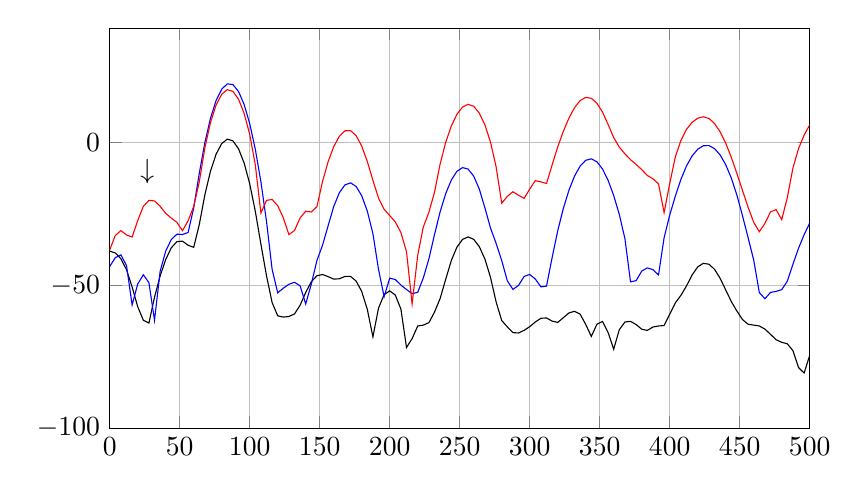
\begin{tikzpicture}

\begin{axis}[%
width=3.5in,
height=2in,
at={(1.011in,0.642in)},
scale only axis,
xmin=0,
xmax=500,
xmajorgrids,
ymin=-100,
ymax=40,
ymajorgrids,
axis background/.style={fill=white}
]
\addplot [color=black,solid,forget plot]
  table[row sep=crcr]{%
0	-38.0274555726395\\
4	-38.651510611096\\
8	-40.6835763316498\\
12	-44.5233654500604\\
16	-50.5494858102553\\
20	-57.4700123218112\\
24	-62.1915564815908\\
28	-63.2015757055571\\
32	-54.1218863275567\\
36	-46.7487138690542\\
40	-40.9467290971577\\
44	-36.8449273638547\\
48	-34.6845233881249\\
52	-34.5213223402229\\
56	-35.9724280699072\\
60	-36.6772737174246\\
64	-28.6674271528343\\
68	-18.217194558207\\
72	-9.98898832926547\\
76	-4.07106545272432\\
80	-0.368076395792921\\
84	1.17496969933739\\
88	0.57648701822052\\
92	-2.18100275090489\\
96	-7.15399795021485\\
100	-14.4358816984991\\
104	-24.0845508427543\\
108	-35.5872503008305\\
112	-46.6533889283533\\
116	-56.0159710677634\\
120	-60.6550679437631\\
124	-61.1055884826112\\
128	-60.8914381351916\\
132	-59.9969714581076\\
136	-56.961622761581\\
140	-52.4685344957774\\
144	-48.7441524039528\\
148	-46.6356131655313\\
152	-46.1873930059594\\
156	-46.9294906633472\\
160	-47.8119777204146\\
164	-47.690591819093\\
168	-46.8825826837565\\
172	-46.8467537669325\\
176	-48.4812066997519\\
180	-52.1230163540569\\
184	-58.4130128830048\\
188	-68.0277111120983\\
192	-57.9616775131286\\
196	-53.2450080795827\\
200	-51.9276258767901\\
204	-53.4022926298902\\
208	-58.2944443907168\\
212	-71.7513621041689\\
216	-68.6214018310109\\
220	-64.226375355091\\
224	-63.9068612395794\\
228	-63.038755922395\\
232	-59.337501072354\\
236	-54.6065716671905\\
240	-47.8602213041462\\
244	-41.3008993018352\\
248	-36.6230946669406\\
252	-33.916708414835\\
256	-33.0403505324789\\
260	-33.8949126465404\\
264	-36.4534736831729\\
268	-40.8004216113336\\
272	-47.2091926461091\\
276	-55.8003263410948\\
280	-62.3018911750458\\
284	-64.5183699939363\\
288	-66.5260434820862\\
292	-66.6689534979108\\
296	-65.7399646598643\\
300	-64.4553768445702\\
304	-62.8090792179468\\
308	-61.5184170600924\\
312	-61.409428082822\\
316	-62.5089007537359\\
320	-62.9672255922981\\
324	-61.3151784822181\\
328	-59.6465779354599\\
332	-59.0805500683714\\
336	-60.0520220813974\\
340	-63.6684212256777\\
344	-67.8650569029938\\
348	-63.6145972565869\\
352	-62.6113255319151\\
356	-66.5332569352241\\
360	-72.3413883143577\\
364	-65.4869930777221\\
368	-62.8241742905383\\
372	-62.603640786007\\
376	-63.7009271841737\\
380	-65.3439536321743\\
384	-65.7621155427093\\
388	-64.5711051161714\\
392	-64.2122257683203\\
396	-64.0517515513743\\
400	-60.0481779467032\\
404	-56.139558664776\\
408	-53.481882026631\\
412	-50.1915366081094\\
416	-46.3459535148488\\
420	-43.5300566698413\\
424	-42.2792601277519\\
428	-42.5902476011542\\
432	-44.3717448113664\\
436	-47.5066147122243\\
440	-51.6149698430641\\
444	-55.6547865192127\\
448	-59.0071528291873\\
452	-61.9659362438547\\
456	-63.6229866445944\\
460	-63.9089786117354\\
464	-64.2017429080807\\
468	-65.312220967396\\
472	-67.1370698885016\\
476	-69.0213987218657\\
480	-69.9237881641573\\
484	-70.4430906235884\\
488	-72.8338583973933\\
492	-78.7585037642878\\
496	-80.6933197777078\\
500	-74.4632736943004\\
504	-70.137881697582\\
508	-67.6291851874067\\
512	-66.0380968106471\\
516	-64.1685585058744\\
520	-61.5993519551501\\
524	-59.1616558907\\
528	-57.8580636404769\\
532	-58.2478511949161\\
536	-60.8975793145943\\
540	-67.3107579802983\\
544	-77.5102035170677\\
548	-69.4470538260138\\
552	-65.9477415578579\\
556	-63.3861497092942\\
560	-62.189659854753\\
564	-63.05419065671\\
568	-66.4441680633171\\
572	-71.7919763266831\\
576	-74.4413599521287\\
580	-69.1442425973303\\
584	-62.2324157968637\\
588	-57.8117479177173\\
592	-55.3099854451853\\
596	-54.3061345310736\\
600	-54.492214457945\\
604	-55.5345697121743\\
608	-57.2129007425673\\
612	-59.611069848711\\
616	-62.8486192253795\\
620	-65.4442229717601\\
624	-64.1611597343069\\
628	-62.0572343559091\\
632	-61.2131948743062\\
636	-61.3723290567409\\
640	-62.2728141000599\\
644	-64.5408708705395\\
648	-69.3891540360687\\
652	-75.2600777076656\\
656	-77.2967418745545\\
660	-73.0885715624367\\
664	-64.2566587198973\\
668	-58.983919626915\\
672	-55.612019762241\\
676	-53.4304509190285\\
680	-52.3352980785938\\
684	-52.3131380776613\\
688	-52.9910755577907\\
692	-53.45994409383\\
696	-53.2232486924585\\
700	-53.0632593649822\\
704	-53.8482035684902\\
708	-56.0268159322002\\
712	-59.9002075018575\\
716	-65.5845051587413\\
720	-71.73880705115\\
724	-73.7305076346682\\
728	-71.7899617026951\\
732	-70.3465628181033\\
736	-69.9235488115039\\
740	-68.3500493510006\\
744	-65.4858938304006\\
748	-63.0990225195289\\
752	-61.6067833505333\\
756	-60.7561831213815\\
760	-59.6135611298982\\
764	-57.6993845370081\\
768	-56.0149856400505\\
772	-55.2990461486835\\
776	-55.6143224667382\\
780	-56.5230422973192\\
784	-56.7655518398845\\
788	-55.5497234204546\\
792	-54.2867612932208\\
796	-54.2374383147607\\
800	-55.9235668640229\\
804	-60.0211339650426\\
808	-69.392783536282\\
812	-68.2774347254717\\
816	-61.8711437691045\\
820	-59.8143591770845\\
824	-59.7085752657574\\
828	-60.5332201184619\\
832	-61.5482356427328\\
836	-62.7970677436238\\
840	-65.4356004016079\\
844	-73.3304802160536\\
848	-75.4632393930567\\
852	-67.2311754838402\\
856	-66.0451411683259\\
860	-67.5172965871505\\
864	-69.9982709325867\\
868	-71.0949444174672\\
872	-69.3751311114515\\
876	-68.1962674719523\\
880	-69.2820852140989\\
884	-69.9732295369882\\
888	-64.942848732347\\
892	-61.8114173339963\\
896	-61.7280359252529\\
900	-63.330397873676\\
904	-62.7084147725373\\
908	-61.1993606250884\\
912	-61.8865060894373\\
916	-66.1352503333639\\
920	-71.3961049590045\\
924	-63.4914316028642\\
928	-59.4893787582751\\
932	-57.6040297101834\\
936	-56.6507025754931\\
940	-56.1513063888604\\
944	-55.9726774405508\\
948	-56.1822319007531\\
952	-56.9715190553563\\
956	-58.5286135286604\\
960	-60.539669180608\\
964	-60.8979436594205\\
968	-59.4488566654333\\
972	-59.2029779860874\\
976	-60.8103860406542\\
980	-63.0984661606324\\
984	-66.8749639868725\\
988	-93.7770054278073\\
992	-63.5962092707241\\
996	-56.9039233691331\\
1000	-54.3012723414932\\
1004	-54.4454133412867\\
1008	-54.5784275824147\\
1012	-51.667584559036\\
1016	-48.9877320534642\\
1020	-47.5648322999433\\
1024	-46.9221756905675\\
1028	-46.6555116232875\\
1032	-46.5808228735464\\
1036	-46.6165858788683\\
1040	-46.7967088368173\\
1044	-47.3352242709638\\
1048	-48.4821045128991\\
1052	-50.2155259347497\\
1056	-52.5980515509452\\
1060	-57.1104362803267\\
1064	-69.2495896880599\\
1068	-70.4230298867048\\
1072	-77.0230701341889\\
1076	-65.6015113082796\\
1080	-58.7495367424867\\
1084	-56.1122384637935\\
1088	-54.6197489660603\\
1092	-53.4888725709275\\
1096	-52.1717658716985\\
1100	-50.4737979360558\\
1104	-48.754576439484\\
1108	-47.2788849377688\\
1112	-46.1278464145447\\
1116	-45.3452827208905\\
1120	-44.9415830862347\\
1124	-44.9059304560528\\
1128	-45.3295453620217\\
1132	-46.3400247415685\\
1136	-47.5972346056926\\
1140	-48.5408768140981\\
1144	-49.9760417805454\\
1148	-52.2960959057686\\
1152	-53.7452214258224\\
1156	-56.9284559619679\\
1160	-62.1983626837934\\
1164	-55.2331246047165\\
1168	-53.6350338568012\\
1172	-54.0785790865471\\
1176	-51.5298711815517\\
1180	-48.2225763742529\\
1184	-45.968866340988\\
1188	-44.7000080450072\\
1192	-44.1590281645503\\
1196	-44.0720625799004\\
1200	-44.2606607154458\\
1204	-44.6643917564106\\
1208	-45.28717366384\\
1212	-46.2578905381685\\
1216	-47.8825121972825\\
1220	-50.1872290624615\\
1224	-52.2964381234626\\
1228	-54.5654138037768\\
1232	-59.4211047759978\\
1236	-59.7320146716102\\
1240	-56.4741031173961\\
1244	-56.104168202275\\
1248	-54.9399498967894\\
1252	-53.4808338164693\\
1256	-53.1969443747193\\
1260	-52.6544665614655\\
1264	-50.8539727315007\\
1268	-48.4204726450024\\
1272	-46.0931974334673\\
1276	-44.2850464014188\\
1280	-43.0415156918079\\
1284	-42.2575078748721\\
1288	-41.8029142436049\\
1292	-41.5748918323117\\
1296	-41.5936590981438\\
1300	-41.9733829068176\\
1304	-42.6435682298194\\
1308	-43.3643245771858\\
1312	-44.5384194363157\\
1316	-47.1375399964247\\
1320	-50.5127252359422\\
1324	-51.4510642997632\\
1328	-54.1626759133009\\
1332	-70.2821383422248\\
1336	-54.9774005959377\\
1340	-51.1457069381935\\
1344	-50.4261659512397\\
1348	-49.8120064355495\\
1352	-49.213892937487\\
1356	-49.0096979174814\\
1360	-48.7202561322586\\
1364	-48.4236043306856\\
1368	-48.609851464664\\
1372	-49.3553403090318\\
1376	-50.4293674656735\\
1380	-51.7709965537079\\
1384	-53.6619618506605\\
1388	-55.3092818999759\\
1392	-54.1670383845034\\
1396	-52.8578967469143\\
1400	-54.0896201647106\\
1404	-56.9737654788055\\
1408	-55.3488048838864\\
1412	-54.3415536399013\\
1416	-57.9689298152135\\
1420	-68.5792142703289\\
1424	-59.3822448331627\\
1428	-56.7946391905853\\
1432	-57.8026494089227\\
1436	-61.3140297633209\\
1440	-65.955517703424\\
1444	-61.2993992378116\\
1448	-56.9982933089461\\
1452	-55.2327447885493\\
1456	-54.9679175852459\\
1460	-55.229544969534\\
1464	-55.4130088771088\\
1468	-55.7857526939584\\
1472	-57.1061803327872\\
1476	-59.4949454704973\\
1480	-60.9348593232694\\
1484	-61.1030610222408\\
1488	-61.1412877238631\\
1492	-58.9500503672795\\
1496	-57.2665596985633\\
1500	-58.2723082223923\\
1504	-62.7450794865743\\
1508	-72.2926587717089\\
1512	-80.2439461450564\\
1516	-66.9658424950025\\
1520	-60.4558247176021\\
1524	-57.574648651393\\
1528	-56.8023980038337\\
1532	-56.9657275917647\\
1536	-57.1277988133015\\
1540	-57.2852728653788\\
1544	-58.0335406400863\\
1548	-59.6972629334685\\
1552	-61.5180105753411\\
1556	-60.9211644011517\\
1560	-59.0392843514323\\
1564	-58.5932470768602\\
1568	-60.6147300881071\\
1572	-65.9827313731715\\
1576	-64.6362009504159\\
1580	-59.9379942535435\\
1584	-59.1633107101623\\
1588	-61.8248112598995\\
1592	-65.2636451481702\\
1596	-63.2562057736505\\
1600	-62.5042611713492\\
1604	-63.4779509561759\\
1608	-63.4058068974005\\
1612	-62.5610840181426\\
1616	-62.1216097501841\\
1620	-61.568411800801\\
1624	-60.7144014544403\\
1628	-60.063203569066\\
1632	-59.9522044033908\\
1636	-60.3876457018285\\
1640	-60.7187939394052\\
1644	-59.9499618398129\\
1648	-58.7496154157564\\
1652	-58.4033836848094\\
1656	-59.0754005891751\\
1660	-59.8077352733209\\
1664	-60.4526711560627\\
1668	-63.4717811596879\\
1672	-72.7300489419727\\
1676	-61.7738788739844\\
1680	-56.9936865219213\\
1684	-55.828525334699\\
1688	-56.7905077495865\\
1692	-58.8955730399589\\
1696	-60.5812521887272\\
1700	-60.1388152933452\\
1704	-58.1014000435503\\
1708	-56.1911550183637\\
1712	-55.145936792147\\
1716	-54.9462014924982\\
1720	-55.4988695337568\\
1724	-56.7290381992657\\
1728	-57.9482795885427\\
1732	-57.9870796943658\\
1736	-57.7063994459606\\
1740	-58.8453749233269\\
1744	-62.7831354631206\\
1748	-71.2585815524349\\
1752	-67.9301050995896\\
1756	-66.5005526093112\\
1760	-73.3680443829787\\
1764	-69.767232784737\\
1768	-62.944242922702\\
1772	-60.8933010836498\\
1776	-60.1028537511172\\
1780	-59.0899460247182\\
1784	-58.6963777225884\\
1788	-59.5325195737462\\
1792	-60.7120465046566\\
1796	-60.6027956009386\\
1800	-59.2804075846378\\
1804	-58.2244518112064\\
1808	-57.8635788435529\\
1812	-57.7636153807415\\
1816	-57.7977063123455\\
1820	-58.7054842328834\\
1824	-61.6906460263396\\
1828	-67.0047562847722\\
1832	-64.9368597592961\\
1836	-62.155324079149\\
1840	-62.570654447902\\
1844	-65.3915861407517\\
1848	-68.0858724316826\\
1852	-67.5873083101635\\
1856	-68.1137044084679\\
1860	-74.238185959802\\
1864	-76.2752168771078\\
1868	-66.0671532072126\\
1872	-62.9907148764615\\
1876	-62.0840625017617\\
1880	-61.6615515847913\\
1884	-61.33308115305\\
1888	-61.2008491115537\\
1892	-60.8694873582207\\
1896	-60.2813707975354\\
1900	-60.0765171582144\\
1904	-60.8023568022474\\
1908	-62.9840088773219\\
1912	-67.0449633586464\\
1916	-67.7833046556872\\
1920	-64.0017440942996\\
1924	-62.9169384400472\\
1928	-65.1643620458734\\
1932	-67.9367999078171\\
1936	-64.7358194498073\\
1940	-62.9736219302299\\
1944	-63.9951322409516\\
1948	-65.6318558754709\\
1952	-63.3386825227192\\
1956	-60.8748372978022\\
1960	-60.0784015113095\\
1964	-60.5504304600666\\
1968	-61.767727995823\\
1972	-63.2661696528192\\
1976	-64.5040726637251\\
1980	-63.2487431603555\\
1984	-60.3180182421082\\
1988	-58.6296215862558\\
1992	-58.8787400921962\\
1996	-61.5520071115623\\
2000	-68.8617800939407\\
2004	-65.7515913023238\\
2008	-58.7249266616689\\
2012	-56.0676211737599\\
2016	-56.1326244518792\\
2020	-58.5866575476027\\
2024	-63.6882244785513\\
2028	-70.9484983190913\\
2032	-68.4101236106035\\
2036	-63.8815697443392\\
2040	-60.5520520450695\\
2044	-58.158550092216\\
2048	-56.5070704749861\\
2052	-55.3135084081071\\
2056	-54.4670923386552\\
2060	-54.1116952476219\\
2064	-54.2237859339789\\
2068	-54.5518536179199\\
2072	-55.3057748946875\\
2076	-57.057112408761\\
2080	-59.9154092378074\\
2084	-62.5158887016593\\
2088	-62.8253063495721\\
2092	-62.2111852647942\\
2096	-61.6340709452282\\
2100	-60.9765321713009\\
2104	-60.7870494520864\\
2108	-61.9909602359863\\
2112	-65.561122484628\\
2116	-71.1200334227455\\
2120	-68.5657530126375\\
2124	-65.5842769379401\\
2128	-65.1029632773355\\
2132	-66.4791122999571\\
2136	-69.16419153044\\
2140	-70.45506655405\\
2144	-69.192472110601\\
2148	-68.6909610175356\\
2152	-69.8781181741165\\
2156	-73.0425575301423\\
2160	-77.4864925077327\\
2164	-75.0456506082266\\
2168	-70.8791649847619\\
2172	-66.9123955292587\\
2176	-62.8373852569631\\
2180	-60.1097733655119\\
2184	-59.3088682462166\\
2188	-60.4902436203128\\
2192	-63.5296112638169\\
2196	-67.7940650482664\\
2200	-71.8372441148372\\
2204	-73.6840821837811\\
2208	-71.9459863662717\\
2212	-69.0575397620188\\
2216	-66.1594307139509\\
2220	-64.3644810730045\\
2224	-64.2012567925309\\
2228	-65.0459354534432\\
2232	-65.0201559141112\\
2236	-63.4739366796754\\
2240	-61.926674928098\\
2244	-61.4391195875663\\
2248	-62.4444576217463\\
2252	-65.4487227707562\\
2256	-73.2462069516213\\
2260	-75.1616102081732\\
2264	-64.7796549395745\\
2268	-61.3684108861175\\
2272	-61.2802598453211\\
2276	-64.6369613202028\\
2280	-68.2833399967633\\
2284	-63.0599854915843\\
2288	-60.3870921768897\\
2292	-60.0622089908533\\
2296	-60.4956739861318\\
2300	-60.0813428318324\\
2304	-58.9943692873587\\
2308	-58.3553180349909\\
2312	-58.1268790491532\\
2316	-57.558097837931\\
2320	-56.4635401430704\\
2324	-55.3927800746486\\
2328	-54.8820598081227\\
2332	-55.2659003813685\\
2336	-56.8252294501309\\
2340	-59.7737531998268\\
2344	-62.4198892783782\\
2348	-60.7836640424831\\
2352	-58.7536433009593\\
2356	-58.5041378799219\\
2360	-60.3003236628672\\
2364	-64.4775500500934\\
2368	-68.1259093511918\\
2372	-65.1868250231584\\
2376	-63.072811308629\\
2380	-62.9486276997308\\
2384	-64.7809750661403\\
2388	-68.6901614794723\\
2392	-73.6530822030932\\
2396	-80.3477143526205\\
};
\addplot [color=blue,solid,forget plot]
  table[row sep=crcr]{%
0	-43.3793333653497\\
4	-40.3104074880648\\
8	-39.3343949048748\\
12	-43.0667070952237\\
16	-56.8593344003102\\
20	-49.5377657318789\\
24	-46.2902680751464\\
28	-49.0254608073622\\
32	-62.2112941351337\\
36	-45.127232545234\\
40	-38.0056148667537\\
44	-33.9338484427806\\
48	-32.0828662152842\\
52	-32.1982917172143\\
56	-31.4821735138688\\
60	-22.8655731909516\\
64	-10.7005925377524\\
68	0.0540293971939503\\
72	8.52262495745948\\
76	14.7081334404157\\
80	18.690352112864\\
84	20.5293089668683\\
88	20.2555253944393\\
92	17.8697457806083\\
96	13.3435663070214\\
100	6.62077602287799\\
104	-2.3778171845483\\
108	-13.743045917769\\
112	-27.6075523993343\\
116	-44.3785135739019\\
120	-52.6093543529198\\
124	-50.9835650985259\\
128	-49.6127856724579\\
132	-48.9214129314788\\
136	-50.1586517401853\\
140	-56.5166402963115\\
144	-49.5426130375589\\
148	-41.2931990878615\\
152	-35.9584353041409\\
156	-29.1425295287302\\
160	-22.4167828598289\\
164	-17.5989777644926\\
168	-14.8519201225955\\
172	-14.1153107263682\\
176	-15.3676549512609\\
180	-18.6366059723657\\
184	-24.0218569707202\\
188	-31.8801018843686\\
192	-44.4019115353234\\
196	-53.9604355397262\\
200	-47.4716612502541\\
204	-47.9622560166994\\
208	-49.9081820064492\\
212	-51.4481420244574\\
216	-52.8987844002606\\
220	-52.4268309247318\\
224	-47.4032528078041\\
228	-40.678373708595\\
232	-32.213613011654\\
236	-24.2783775098433\\
240	-17.8892964036151\\
244	-13.1445435045851\\
248	-10.0847345912792\\
252	-8.7757067402525\\
256	-9.30067268067702\\
260	-11.7700418769846\\
264	-16.3152552441688\\
268	-22.8676079973536\\
272	-29.9371903897859\\
276	-35.2952556496479\\
280	-41.3013989899267\\
284	-48.391148516396\\
288	-51.4051281166252\\
292	-50.0047091263776\\
296	-46.8873838865238\\
300	-46.1725893016671\\
304	-47.7839415451967\\
308	-50.5179705611921\\
312	-50.2662163599615\\
316	-40.2847079657027\\
320	-30.9121020781833\\
324	-23.0969634916931\\
328	-16.7335730289225\\
332	-11.7722112422993\\
336	-8.2498182628668\\
340	-6.22050884783891\\
344	-5.71681144250457\\
348	-6.74257597357052\\
352	-9.27142079184058\\
356	-13.2434536005644\\
360	-18.5661698976219\\
364	-25.1883206299739\\
368	-33.6507199782958\\
372	-48.7684801760672\\
376	-48.3533606009608\\
380	-45.0055042272334\\
384	-43.8831264111822\\
388	-44.505011241597\\
392	-46.3587900589017\\
396	-33.2871522072958\\
400	-25.4133197391412\\
404	-18.7857089099903\\
408	-12.9041000763319\\
412	-8.19030875825299\\
416	-4.6927309754909\\
420	-2.35154989111149\\
424	-1.14333965070649\\
428	-1.06741014323903\\
432	-2.12932068882579\\
436	-4.34708559916792\\
440	-7.76243282597698\\
444	-12.4413729451656\\
448	-18.4423525233541\\
452	-25.6466737740787\\
456	-33.3316753603064\\
460	-41.1529404152644\\
464	-52.4985526909053\\
468	-54.6808743870508\\
472	-52.4585222168964\\
476	-52.1172280014828\\
480	-51.4949103360752\\
484	-48.5209498649854\\
488	-42.608642685797\\
492	-37.0273393090303\\
496	-32.2659757001395\\
500	-28.1587681429875\\
504	-24.7034795885027\\
508	-21.9590070953369\\
512	-19.9592761228645\\
516	-18.7019187405112\\
520	-18.160621090324\\
524	-18.3088621145862\\
528	-19.1650629425827\\
532	-20.8597405986809\\
536	-23.7099324155317\\
540	-28.3497794729038\\
544	-36.055274181805\\
548	-44.0523877096354\\
552	-43.6738325735485\\
556	-47.6415397601959\\
560	-51.674159829837\\
564	-45.7727669400794\\
568	-41.2630229263906\\
572	-39.210442353446\\
576	-37.4791129177693\\
580	-34.642868441494\\
584	-31.6496130672136\\
588	-29.2056856928665\\
592	-27.3182612539967\\
596	-25.9793686476967\\
600	-25.24402199331\\
604	-25.1292855250358\\
608	-25.6143395160166\\
612	-26.6907790201062\\
616	-28.3990307775905\\
620	-30.8087213546125\\
624	-33.8371086255296\\
628	-37.1282646437246\\
632	-39.9216767415908\\
636	-41.9198972231072\\
640	-45.3561965057236\\
644	-43.401610440659\\
648	-41.7465223669117\\
652	-40.1135304210367\\
656	-37.481234481949\\
660	-35.0013974218215\\
664	-32.1736879074796\\
668	-30.0041898906898\\
672	-28.7948191153829\\
676	-28.4494523349263\\
680	-28.9550431951451\\
684	-30.3782451679085\\
688	-32.8276887878465\\
692	-36.3869180643404\\
696	-40.6469317934961\\
700	-43.8460476335852\\
704	-45.8024861600988\\
708	-49.0913005855115\\
712	-56.0593884504153\\
716	-65.4782241106255\\
720	-63.8454294569943\\
724	-69.4073591721873\\
728	-69.4886651960317\\
732	-57.4286855134977\\
736	-49.8592902473402\\
740	-46.8923724311517\\
744	-47.2924831138272\\
748	-46.8889458579998\\
752	-41.5526601133183\\
756	-37.2964656779155\\
760	-34.4817387776398\\
764	-32.4297100124371\\
768	-30.8237288533105\\
772	-29.6993943474942\\
776	-29.2562958295557\\
780	-29.7003678108406\\
784	-31.1343798576777\\
788	-33.2594857375315\\
792	-35.1162238438634\\
796	-36.484312767024\\
800	-37.9389996580759\\
804	-39.6619894728682\\
808	-44.7838133302906\\
812	-52.6493762076393\\
816	-39.7402734881509\\
820	-35.9929503103073\\
824	-34.0515931270673\\
828	-32.3738546597342\\
832	-29.6853133422157\\
836	-26.1105753686617\\
840	-22.905658221372\\
844	-20.4428317097388\\
848	-18.6933715169628\\
852	-17.5828632654678\\
856	-17.0425879448727\\
860	-17.0379082595022\\
864	-17.5920438019755\\
868	-18.8202006919413\\
872	-20.985758149233\\
876	-24.5372792473756\\
880	-30.1422283303192\\
884	-38.4941739586769\\
888	-39.1675959820217\\
892	-35.9770636412854\\
896	-35.9837951938162\\
900	-37.6507840707315\\
904	-36.4546285898191\\
908	-31.8307518074081\\
912	-29.5673028948434\\
916	-26.7267207339616\\
920	-22.1641188150572\\
924	-18.8038016897896\\
928	-16.8931535702649\\
932	-15.9616065153281\\
936	-15.6074692762265\\
940	-15.7067777165691\\
944	-16.4405199649414\\
948	-17.995627202956\\
952	-20.236624287773\\
956	-22.5528204447799\\
960	-24.3467409555328\\
964	-25.8417998422323\\
968	-28.3030980080263\\
972	-30.7982834094398\\
976	-29.1492915118198\\
980	-30.7322391576134\\
984	-46.7786617255289\\
988	-34.3185154076249\\
992	-31.4994064141801\\
996	-29.471947845708\\
1000	-26.2020277397225\\
1004	-24.1162608878236\\
1008	-22.7774954804273\\
1012	-21.6124033413948\\
1016	-20.4382114401136\\
1020	-19.6318822809056\\
1024	-19.5111549108456\\
1028	-20.0662846616352\\
1032	-21.1821291935389\\
1036	-22.7998722631442\\
1040	-24.969897238222\\
1044	-27.7791222122827\\
1048	-31.0237547970521\\
1052	-33.9795365548093\\
1056	-35.5876768800113\\
1060	-36.0104428196091\\
1064	-38.5366062876057\\
1068	-46.6676251410762\\
1072	-41.6840477305458\\
1076	-37.940817026508\\
1080	-35.5455435648283\\
1084	-33.1089360149878\\
1088	-31.4112712147719\\
1092	-29.7619984358559\\
1096	-28.2431184154168\\
1100	-27.4767973175203\\
1104	-27.5369182647338\\
1108	-28.1977854758007\\
1112	-29.2081675384176\\
1116	-30.3518829691763\\
1120	-31.4766566046055\\
1124	-32.5504742869138\\
1128	-33.9429754849402\\
1132	-36.3337696764089\\
1136	-37.7598431027261\\
1140	-35.6332110889659\\
1144	-35.1812858974422\\
1148	-38.7123757190464\\
1152	-49.9803034826085\\
1156	-54.9234350249867\\
1160	-46.6693080385205\\
1164	-39.0938078790283\\
1168	-35.5478265256394\\
1172	-34.7837490630541\\
1176	-36.0469638739989\\
1180	-39.4433693162365\\
1184	-45.3819185903671\\
1188	-46.1932906690418\\
1192	-43.8421185270868\\
1196	-44.7188637291212\\
1200	-47.7256844593601\\
1204	-50.2039792052004\\
1208	-50.3599426535444\\
1212	-45.3363154883364\\
1216	-41.1751306692493\\
1220	-39.7800768530546\\
1224	-40.3817272041452\\
1228	-41.2514162330106\\
1232	-39.7015757304511\\
1236	-36.4174054035097\\
1240	-34.3396832873636\\
1244	-34.4971016331685\\
1248	-37.5279976614601\\
1252	-47.1007051847878\\
1256	-44.1438351026218\\
1260	-35.0266469531028\\
1264	-30.7174847282733\\
1268	-28.382451052974\\
1272	-27.3726294512991\\
1276	-27.5028960486777\\
1280	-28.6818613763131\\
1284	-30.7200838059278\\
1288	-33.2735019616364\\
1292	-34.6129820901356\\
1296	-32.2424149238019\\
1300	-29.1615018612742\\
1304	-27.9483187275349\\
1308	-29.0239222059131\\
1312	-31.673658060613\\
1316	-33.8859026741715\\
1320	-34.534098933047\\
1324	-33.248888652925\\
1328	-32.3473560820903\\
1332	-32.5171939460971\\
1336	-32.1461269545508\\
1340	-32.4015895031074\\
1344	-35.7334967275228\\
1348	-46.6960270281217\\
1352	-45.6698458965438\\
1356	-40.5171558524363\\
1360	-39.7953987048741\\
1364	-39.2664310604665\\
1368	-38.2786483959244\\
1372	-37.4362082190928\\
1376	-36.7642724702497\\
1380	-35.6939420086857\\
1384	-34.2415204792634\\
1388	-33.3460212046781\\
1392	-33.6907264000125\\
1396	-34.3413017470434\\
1400	-33.3600559652187\\
1404	-32.6834024159628\\
1408	-34.7017083496984\\
1412	-41.320721371547\\
1416	-41.1809979065804\\
1420	-36.5447164059511\\
1424	-36.0924184916698\\
1428	-37.205354804001\\
1432	-36.5692406595394\\
1436	-34.814231261706\\
1440	-33.8527291854732\\
1444	-33.7335796392769\\
1448	-34.2362643966751\\
1452	-35.430733564662\\
1456	-37.6158553424706\\
1460	-41.2635634767616\\
1464	-46.4199174735935\\
1468	-51.3029258991769\\
1472	-68.9312431838497\\
1476	-45.8015124690331\\
1480	-39.9528142701708\\
1484	-38.4486268329344\\
1488	-39.7017979204687\\
1492	-41.7066702949979\\
1496	-42.1311363950127\\
1500	-43.6902832679481\\
1504	-50.0699595158331\\
1508	-62.4433698223954\\
1512	-51.6445363307665\\
1516	-52.8820156711677\\
1520	-52.1275507359403\\
1524	-46.8584583255144\\
1528	-44.237431584167\\
1532	-43.4797840278924\\
1536	-43.5448881706329\\
1540	-43.1731442909405\\
1544	-42.1305321135139\\
1548	-41.3993419142891\\
1552	-41.1384776417632\\
1556	-40.6134518930494\\
1560	-39.7421769424453\\
1564	-39.3916401712373\\
1568	-40.4221677240796\\
1572	-43.5448681247163\\
1576	-49.1945211753609\\
1580	-54.2071665173561\\
1584	-54.5113885334975\\
1588	-51.9293909081478\\
1592	-47.2470171152513\\
1596	-43.5862229977316\\
1600	-41.297946584517\\
1604	-40.1858887865353\\
1608	-39.95996342474\\
1612	-40.0364617344045\\
1616	-39.714680846606\\
1620	-39.1209561234104\\
1624	-39.1440025496384\\
1628	-40.1337322567669\\
1632	-41.2415195641443\\
1636	-41.1387863128901\\
1640	-40.1611186863529\\
1644	-39.1780451476729\\
1648	-38.5091950566943\\
1652	-38.4406782068308\\
1656	-39.275700011611\\
1660	-40.7517937177982\\
1664	-42.0610057862875\\
1668	-43.311806307408\\
1672	-45.4882902731927\\
1676	-49.119908148701\\
1680	-49.2485405243858\\
1684	-45.0966284990019\\
1688	-43.0777913450606\\
1692	-43.6734911746418\\
1696	-47.1047204851452\\
1700	-53.5413462113875\\
1704	-53.90996374643\\
1708	-49.3085158025794\\
1712	-45.5248319038693\\
1716	-42.7109542475869\\
1720	-40.9650492425755\\
1724	-40.1295532834476\\
1728	-39.7548282076696\\
1732	-39.1359386025259\\
1736	-38.0870545350802\\
1740	-37.1948851426132\\
1744	-37.1196718975624\\
1748	-38.3813266032709\\
1752	-41.4782021543896\\
1756	-47.123814870517\\
1760	-55.1853923056855\\
1764	-54.2215113840618\\
1768	-50.4050982857326\\
1772	-47.3364536355384\\
1776	-45.7680261531044\\
1780	-46.0356660913151\\
1784	-47.9067816018557\\
1788	-50.2435269645061\\
1792	-50.4065642764461\\
1796	-46.9769020780493\\
1800	-43.155202907089\\
1804	-40.6900930154162\\
1808	-39.6237203192433\\
1812	-39.7211431391672\\
1816	-40.7315048723526\\
1820	-42.2720922302826\\
1824	-43.6420245404219\\
1828	-44.2131694497876\\
1832	-44.1107296394363\\
1836	-43.875146238833\\
1840	-44.0366122252439\\
1844	-44.8889255172476\\
1848	-46.3904590030166\\
1852	-48.0466717988562\\
1856	-48.5895001521002\\
1860	-47.7914939592902\\
1864	-47.1289272146687\\
1868	-46.9773444669621\\
1872	-46.6696071399298\\
1876	-45.7888976914351\\
1880	-44.6925371750158\\
1884	-43.8216065694593\\
1888	-43.5980200899648\\
1892	-44.4114163646312\\
1896	-45.2886020873062\\
1900	-43.6061291379996\\
1904	-41.157342804694\\
1908	-39.9966191518026\\
1912	-40.4466147849386\\
1916	-42.7129116309631\\
1920	-47.5293646467304\\
1924	-56.6184446173826\\
1928	-53.6598405560101\\
1932	-49.8274396579189\\
1936	-49.3415981992721\\
1940	-51.0332633223516\\
1944	-54.6947214574421\\
1948	-57.7392492830673\\
1952	-53.5253517120251\\
1956	-48.7329500637986\\
1960	-45.4162462017859\\
1964	-43.6506575298472\\
1968	-43.327160914285\\
1972	-43.7706696798571\\
1976	-43.8853771843637\\
1980	-43.5614552983897\\
1984	-43.526917040746\\
1988	-44.1120114354727\\
1992	-45.2625175792014\\
1996	-46.9581344859802\\
2000	-49.6073316323388\\
2004	-54.1684050401325\\
2008	-58.2132145770142\\
2012	-53.7604682420787\\
2016	-50.8723798262948\\
2020	-50.7589080423325\\
2024	-53.0326241497676\\
2028	-51.7396910575994\\
2032	-47.1184440768288\\
2036	-44.7801648135784\\
2040	-44.5777417285831\\
2044	-45.6586220894999\\
2048	-46.3349222445907\\
2052	-45.2068202838084\\
2056	-43.4003060175184\\
2060	-42.0567538666727\\
2064	-41.3632341323322\\
2068	-41.0195900150956\\
2072	-40.4360492738271\\
2076	-39.4236786417379\\
2080	-38.6719029817232\\
2084	-39.0553378891916\\
2088	-41.209560381275\\
2092	-45.8806134501815\\
2096	-53.5837519363167\\
2100	-50.6630039280609\\
2104	-46.8784803447698\\
2108	-45.6960584336912\\
2112	-45.9601342708314\\
2116	-46.8670445976655\\
2120	-47.4656990272437\\
2124	-47.0041569099676\\
2128	-45.6866653851499\\
2132	-44.248062741998\\
2136	-43.1773430089917\\
2140	-42.596560284208\\
2144	-42.6275967673126\\
2148	-43.693841016409\\
2152	-46.1423625647962\\
2156	-48.848150034963\\
2160	-49.0181783675961\\
2164	-48.0800192847049\\
2168	-47.7105605957354\\
2172	-48.3400959159663\\
2176	-50.34866692126\\
2180	-53.6322880121244\\
2184	-57.6181642015383\\
2188	-59.2131811944603\\
2192	-55.1233607608916\\
2196	-51.8008863031934\\
2200	-50.2517953478432\\
2204	-50.6991760092347\\
2208	-53.9398806862808\\
2212	-60.246927875092\\
2216	-55.1473176435103\\
2220	-49.7153135327897\\
2224	-46.7268057565256\\
2228	-45.2295751193025\\
2232	-44.5961797061741\\
2236	-44.3163575914134\\
2240	-44.3210829268774\\
2244	-45.0595652735571\\
2248	-47.2871249159291\\
2252	-52.0928656657296\\
2256	-55.8043544306014\\
2260	-50.2282721705792\\
2264	-46.5061991352952\\
2268	-44.5032051222647\\
2272	-43.8224298256469\\
2276	-44.3303209452262\\
2280	-45.9831161075589\\
2284	-49.4975152715889\\
2288	-58.5146722336647\\
2292	-56.2130727028928\\
2296	-50.0594630122668\\
2300	-48.7154885637919\\
2304	-49.4825879471138\\
2308	-51.7902352823369\\
2312	-54.5120462088715\\
2316	-53.2385832328784\\
2320	-52.3843925330739\\
2324	-52.7279119803419\\
2328	-49.1875255968379\\
2332	-45.8908932845971\\
2336	-45.2667140005565\\
2340	-47.8068125848763\\
2344	-56.7561241299407\\
2348	-56.1044062185524\\
2352	-48.0679669994204\\
2356	-45.4408746065714\\
2360	-45.1877366025854\\
2364	-47.0195449765416\\
2368	-51.6385522380725\\
2372	-54.876903196434\\
2376	-48.5819614646499\\
2380	-45.3543873558628\\
2384	-44.9442627016261\\
2388	-47.1361596275073\\
2392	-52.9160957208032\\
2396	-73.6690631663724\\
};
\addplot [color=red,solid,forget plot]
  table[row sep=crcr]{%
0	-37.593202458105\\
4	-32.5387620443458\\
8	-30.8122841430479\\
12	-32.3599186192166\\
16	-33.0814041560757\\
20	-27.3382090481522\\
24	-22.3550263121014\\
28	-20.2431715022246\\
32	-20.4478651256333\\
36	-22.2909561360892\\
40	-24.7778068037207\\
44	-26.4864644904208\\
48	-27.9352355388885\\
52	-30.8434918572424\\
56	-27.3904054365501\\
60	-22.3669535015182\\
64	-13.7119724899118\\
68	-1.82104793749142\\
72	6.99979737099748\\
76	13.1271643908763\\
80	16.9083414163075\\
84	18.4847148598002\\
88	17.9066797109304\\
92	15.1710945949398\\
96	10.215897639397\\
100	2.83532884438976\\
104	-7.80916972141651\\
108	-24.6797794214996\\
112	-20.2659761298403\\
116	-19.9063066044904\\
120	-22.133287492316\\
124	-26.3265168445164\\
128	-32.2431142676205\\
132	-30.7882390969197\\
136	-26.3977287201758\\
140	-24.0529377707577\\
144	-24.3126147792817\\
148	-22.4435311972716\\
152	-13.6775856756861\\
156	-6.72906827540472\\
160	-1.47445796756258\\
164	2.17925153517975\\
168	4.09145142698227\\
172	4.17469841481913\\
176	2.39127573909082\\
180	-1.25556885865565\\
184	-6.64881927350287\\
188	-13.2481389231124\\
192	-19.435261172533\\
196	-23.3631549365996\\
200	-25.5575118824393\\
204	-27.8130911659649\\
208	-31.5556407533074\\
212	-38.2043570244905\\
216	-56.5029923341118\\
220	-39.4698467250608\\
224	-29.5557758777701\\
228	-24.4056665338882\\
232	-17.3763869501723\\
236	-7.55094049522068\\
240	0.0822412084247637\\
244	5.7671305083178\\
248	9.86282489805806\\
252	12.4150719676784\\
256	13.370613665883\\
260	12.6774662093547\\
264	10.2935007047063\\
268	6.15806156579304\\
272	0.100392640540774\\
276	-8.54614956783542\\
280	-21.2252347760262\\
284	-18.8490519800895\\
288	-17.2478940671731\\
292	-18.4380372340826\\
296	-19.5657262054174\\
300	-16.2979988357667\\
304	-13.3408820835405\\
308	-13.7686540877533\\
312	-14.3610081973573\\
316	-7.86797480242334\\
320	-1.55123351110673\\
324	3.89995840052385\\
328	8.51889582152401\\
332	12.1983993481039\\
336	14.6741139612462\\
340	15.785572451455\\
344	15.4828825362641\\
348	13.7546750739755\\
352	10.6245372070125\\
356	6.29832705901459\\
360	1.70938959509664\\
364	-1.6207205462543\\
368	-3.96978466811951\\
372	-6.00729963670208\\
376	-7.68528228475012\\
380	-9.48584559726435\\
384	-11.5326372146752\\
388	-12.6884761260448\\
392	-14.4730230240182\\
396	-24.5104105868142\\
400	-14.3802508490155\\
404	-5.04724660040584\\
408	0.727036187689978\\
412	4.60596461549798\\
416	7.05765813635985\\
420	8.51057908707\\
424	9.00932393736888\\
428	8.41538994515072\\
432	6.66223937899442\\
436	3.76055778280686\\
440	-0.233145035856987\\
444	-5.18790093729145\\
448	-10.8440227372476\\
452	-16.8180910580305\\
456	-22.6684035723433\\
460	-27.9479977294683\\
464	-31.2352395298811\\
468	-28.3093503814691\\
472	-24.2672237645743\\
476	-23.4792368517034\\
480	-26.9951694417109\\
484	-19.2790146778995\\
488	-8.95438146545842\\
492	-2.14457706833809\\
496	2.60712963334266\\
500	6.14522059636192\\
504	8.97305350710479\\
508	11.1796778493197\\
512	12.655048171575\\
516	13.3079584911332\\
520	13.0773828339101\\
524	11.909036688435\\
528	9.77739472278366\\
532	6.7281920759796\\
536	2.90414973740291\\
540	-1.5332869498723\\
544	-6.60737200197449\\
548	-12.7519788182467\\
552	-20.3264594817459\\
556	-22.6311149384314\\
560	-19.2381868589412\\
564	-20.7713649901769\\
568	-34.467294223206\\
572	-15.9573307506509\\
576	-11.0823735694285\\
580	-8.61703351001005\\
584	-6.95294268190114\\
588	-5.70203523197833\\
592	-4.78289079552993\\
596	-4.16394754642475\\
600	-3.78560801418243\\
604	-3.58166394004822\\
608	-3.55990938003204\\
612	-3.84204771778599\\
616	-4.69184407367303\\
620	-6.62131605958592\\
624	-10.2038482590334\\
628	-14.753819870162\\
632	-17.6490825816842\\
636	-16.2967055247829\\
640	-21.1973891158265\\
644	-14.9276850014572\\
648	-8.91882424266648\\
652	-8.0884944442303\\
656	-4.90464170519531\\
660	-0.284046812084207\\
664	3.44309859470965\\
668	6.21952057614182\\
672	8.02395133045615\\
676	8.98267904877006\\
680	9.26684626648538\\
684	8.96573484709702\\
688	8.08410578123186\\
692	6.61822757351692\\
696	4.62659325606842\\
700	2.28135230304298\\
704	-0.165881650625083\\
708	-2.67454884736289\\
712	-5.37843813515203\\
716	-8.853769377101\\
720	-14.7844131061547\\
724	-16.585192329122\\
728	-14.3872327089371\\
732	-14.9137031892981\\
736	-18.561763482303\\
740	-9.77303646390669\\
744	-4.74484893910102\\
748	-2.2710170619697\\
752	-0.244518409926444\\
756	1.40015589648481\\
760	2.22544791388275\\
764	2.31843199462608\\
768	1.98966788179592\\
772	1.42692526694565\\
776	0.643549525101541\\
780	-0.357799726905412\\
784	-1.50490086112325\\
788	-2.88758349587211\\
792	-5.13828251195144\\
796	-8.64535439316524\\
800	-12.8159744819632\\
804	-18.012254587252\\
808	-18.236952852185\\
812	-28.9714444806249\\
816	-8.12001273325709\\
820	-2.48977632789087\\
824	-0.0635637130379939\\
828	1.71919411272239\\
832	3.7667486456229\\
836	6.02736714511627\\
840	8.0656169126697\\
844	9.50974415679797\\
848	10.3510199334089\\
852	10.7455036610759\\
856	10.7924507716151\\
860	10.4939110740861\\
864	9.83218717855051\\
868	8.83583090266306\\
872	7.53150132197859\\
876	5.89765503473516\\
880	4.11410764363244\\
884	2.4526217685597\\
888	0.519421741503794\\
892	-1.99054845299254\\
896	-6.61690720706157\\
900	-15.4895984479228\\
904	-5.34589549205052\\
908	-3.00267404236103\\
912	-0.135470281689124\\
916	3.6712062988841\\
920	6.53960704706391\\
924	9.27916622407563\\
928	11.6338217794535\\
932	13.105086260896\\
936	13.7578545591878\\
940	13.890251987486\\
944	13.7018347872785\\
948	13.1688146419644\\
952	12.1787079516313\\
956	10.6129838923048\\
960	8.24785516578569\\
964	5.42322419371403\\
968	3.50893510952147\\
972	0.372788129263664\\
976	-5.45116581891294\\
980	-2.09404272254131\\
984	-3.53243753180216\\
988	-0.27824129469636\\
992	5.08644571272517\\
996	7.49833865871785\\
1000	9.39928473763364\\
1004	11.1753731004283\\
1008	12.4516674689085\\
1012	13.3796592423684\\
1016	14.0040729706159\\
1020	14.1618712111014\\
1024	13.8112638063281\\
1028	13.0453506913286\\
1032	11.9595561401707\\
1036	10.6679046372591\\
1040	9.21777091212992\\
1044	7.24668214760669\\
1048	4.93747106918826\\
1052	4.00598994818247\\
1056	2.39938123774494\\
1060	-3.58429705208681\\
1064	-2.32501930322203\\
1068	0.146425980100884\\
1072	-2.90273344494612\\
1076	-1.06850296435607\\
1080	3.07307222163131\\
1084	5.08080736418341\\
1088	6.42230106600414\\
1092	7.24352696400452\\
1096	7.61829742472202\\
1100	7.91258772114697\\
1104	8.09026838154747\\
1108	7.85840166673046\\
1112	7.1021788379623\\
1116	5.93444912786063\\
1120	4.65248471319524\\
1124	3.33260702049799\\
1128	1.52104545965663\\
1132	0.0555870181289817\\
1136	0.415714236871292\\
1140	-0.737546851770428\\
1144	-6.10005480693188\\
1148	-3.83090930469899\\
1152	-1.04380568639799\\
1156	-4.14922919765482\\
1160	-4.75014469986619\\
1164	0.783162210582858\\
1168	2.94545809453509\\
1172	4.19802245293881\\
1176	5.51027537468856\\
1180	6.42154808887962\\
1184	6.94771016178456\\
1188	7.26534166546208\\
1192	7.21528987276464\\
1196	6.59135851913241\\
1200	5.51884605557795\\
1204	4.52056146170018\\
1208	3.66079936022354\\
1212	2.20821518634498\\
1216	1.12297679601377\\
1220	2.06392746843169\\
1224	1.38785272517869\\
1228	-3.75260826076278\\
1232	-1.08353535343369\\
1236	2.60926190746109\\
1240	0.343394067983434\\
1244	-1.7697706630987\\
1248	5.32278959323501\\
1252	8.19296784430342\\
1256	9.08332448373373\\
1260	9.9666575622091\\
1264	10.9506752249834\\
1268	11.5852873971462\\
1272	12.1584464135313\\
1276	12.7738736342466\\
1280	13.0753634575796\\
1284	12.9437955851991\\
1288	12.57261380258\\
1292	11.9289881804053\\
1296	10.6649999317753\\
1300	8.94372952253817\\
1304	8.12005674839399\\
1308	7.60206476042607\\
1312	4.71268571270319\\
1316	-0.456774382866717\\
1320	2.67059329397186\\
1324	3.95874066240455\\
1328	0.824655918019552\\
1332	-0.687909730074696\\
1336	3.63359474970903\\
1340	5.40950915269097\\
1344	5.56090857513574\\
1348	5.46943849429314\\
1352	5.54202601818258\\
1356	5.63414580564146\\
1360	5.73012293647313\\
1364	5.72444809358543\\
1368	5.598770656667\\
1372	5.5111203261128\\
1376	5.22081559124379\\
1380	4.35841573464474\\
1384	3.52007451586727\\
1388	3.88708847695822\\
1392	4.12954238940121\\
1396	2.36165436027696\\
1400	-0.327675424245874\\
1404	1.51865869070964\\
1408	2.71951608518762\\
1412	-0.118617102276289\\
1416	-8.43351596585285\\
1420	-0.763045634592818\\
1424	2.94956344884856\\
1428	3.25556288099509\\
1432	2.19244933259461\\
1436	1.55821041808607\\
1440	1.49899875699214\\
1444	1.18013037717623\\
1448	0.694550472105588\\
1452	0.53315294936273\\
1456	0.692693044584557\\
1460	0.429616119029557\\
1464	-0.949310409025922\\
1468	-2.97990503485173\\
1472	-3.49404168927032\\
1476	-3.17357238713952\\
1480	-5.02210614307616\\
1484	-10.8710578738464\\
1488	-9.9515361960161\\
1492	-6.47891603099894\\
1496	-7.88716677817667\\
1500	-11.7223586420207\\
1504	-7.00210098466116\\
1508	-3.68148574282418\\
1512	-3.14393527889375\\
1516	-4.32996086343858\\
1520	-6.16281436871192\\
1524	-7.61999697462754\\
1528	-8.59837107097429\\
1532	-9.28393125580703\\
1536	-9.43650186890039\\
1540	-9.1351551962444\\
1544	-9.07893681554527\\
1548	-9.9276826849661\\
1552	-11.7857990846827\\
1556	-14.1886450475913\\
1560	-16.3824591441135\\
1564	-17.904012443993\\
1568	-18.5114985249652\\
1572	-18.7082759875665\\
1576	-20.1468660390226\\
1580	-24.6473941432566\\
1584	-32.0010279572789\\
1588	-24.9691390616032\\
1592	-20.2015635917843\\
1596	-16.633641011631\\
1600	-13.6670504563651\\
1604	-11.5614617693205\\
1608	-10.3175033077121\\
1612	-9.68455618222471\\
1616	-9.35629901013372\\
1620	-9.21233393582157\\
1624	-9.45647951572953\\
1628	-10.4182031830708\\
1632	-12.1253520509155\\
1636	-13.7176209708852\\
1640	-13.6962462252711\\
1644	-12.7597643666061\\
1648	-12.7302372686589\\
1652	-14.3356712458723\\
1656	-16.3467136850239\\
1660	-15.2022237560294\\
1664	-13.7291322346654\\
1668	-14.8981397150452\\
1672	-20.6440322360749\\
1676	-22.0547609772657\\
1680	-14.873022113892\\
1684	-12.0689286859705\\
1688	-11.2164387272027\\
1692	-10.8835704750838\\
1696	-10.3220781168904\\
1700	-9.74783564029991\\
1704	-9.47708068117976\\
1708	-9.67896629686109\\
1712	-10.4769415954922\\
1716	-12.7061423268501\\
1720	-15.9747723496557\\
1724	-13.9128451842793\\
1728	-11.2481458895844\\
1732	-10.7023877218452\\
1736	-12.6573589078795\\
1740	-20.680214759651\\
1744	-19.8801385208749\\
1748	-12.4657171033932\\
1752	-11.9768069645209\\
1756	-17.3404096386525\\
1760	-16.414125303551\\
1764	-8.65069177672065\\
1768	-5.15965932244339\\
1772	-3.5611882184575\\
1776	-3.00224926243412\\
1780	-3.01150642531111\\
1784	-3.26981130971479\\
1788	-3.70451905297733\\
1792	-4.52363273547217\\
1796	-6.01669516423617\\
1800	-8.36282924022099\\
1804	-11.4593333274433\\
1808	-14.2950754104954\\
1812	-15.0707914625854\\
1816	-14.6041502278842\\
1820	-14.7864267003527\\
1824	-16.4601786101473\\
1828	-20.2814352638902\\
1832	-25.2885580898563\\
1836	-21.8130169846889\\
1840	-18.4669532155386\\
1844	-17.8293713505215\\
1848	-19.9738534646667\\
1852	-25.8418904999689\\
1856	-26.0591349747573\\
1860	-21.7596351020348\\
1864	-20.3201800974511\\
1868	-19.6486717412735\\
1872	-18.7882369877988\\
1876	-18.5101449145228\\
1880	-19.7700195212451\\
1884	-21.6930838626926\\
1888	-20.8536286641801\\
1892	-19.1916879062029\\
1896	-18.8827191889062\\
1900	-19.9046509471604\\
1904	-22.5646631310896\\
1908	-29.0563125973281\\
1912	-30.4818685127947\\
1916	-23.0321726727566\\
1920	-20.8296449597531\\
1924	-22.1876824177272\\
1928	-29.1205294228348\\
1932	-31.2871919010575\\
1936	-21.6142337930654\\
1940	-18.0050676678316\\
1944	-16.3255656682785\\
1948	-15.3946473287885\\
1952	-14.7347401169003\\
1956	-14.4127685061621\\
1960	-14.8070400627777\\
1964	-16.3134689662898\\
1968	-19.1316419937067\\
1972	-22.9201505794272\\
1976	-26.191863994967\\
1980	-26.8207331439989\\
1984	-25.657194640123\\
1988	-25.3358937536323\\
1992	-26.363126347269\\
1996	-26.9284291635017\\
2000	-26.4873554499995\\
2004	-28.2703947040917\\
2008	-39.3350712138754\\
2012	-28.5378370652776\\
2016	-21.6586545246181\\
2020	-18.8383799949644\\
2024	-17.9602477726771\\
2028	-17.8969102096994\\
2032	-17.5382343253768\\
2036	-17.0282242575855\\
2040	-17.3558513154646\\
2044	-19.1138277172078\\
2048	-22.6490554438048\\
2052	-26.0943082799654\\
2056	-24.2302192696776\\
2060	-22.3919555378699\\
2064	-21.6720036504779\\
2068	-20.7190202987462\\
2072	-19.7502256829875\\
2076	-19.5359980144942\\
2080	-19.8674277102326\\
2084	-19.419414690448\\
2088	-17.8164814488317\\
2092	-16.6934820630976\\
2096	-17.0335089085218\\
2100	-18.771094039963\\
2104	-20.4633656256017\\
2108	-20.3352187173495\\
2112	-19.398643383136\\
2116	-18.3570788757947\\
2120	-17.3319556407207\\
2124	-16.8408864233045\\
2128	-17.3464930893419\\
2132	-19.0996309468883\\
2136	-22.1784877068494\\
2140	-26.1786493734759\\
2144	-29.3983264557016\\
2148	-29.9674956863831\\
2152	-29.6625112725677\\
2156	-31.1137328087583\\
2160	-34.9380118577614\\
2164	-29.816417906415\\
2168	-23.5260749986041\\
2172	-20.2480159752508\\
2176	-19.4817615420899\\
2180	-21.4344150552472\\
2184	-26.9349019822303\\
2188	-26.137008234543\\
2192	-21.8114570117171\\
2196	-21.2008533132702\\
2200	-22.4443902653289\\
2204	-22.4990943393714\\
2208	-21.6746240502601\\
2212	-21.9050347148822\\
2216	-23.20390131189\\
2220	-25.1362589788874\\
2224	-27.1380468660732\\
2228	-27.3020746843295\\
2232	-24.6451989673537\\
2236	-21.6120571014274\\
2240	-19.9568784980999\\
2244	-20.4132385957172\\
2248	-22.4884552499488\\
2252	-20.8257939592462\\
2256	-16.4450764748407\\
2260	-13.5016479184298\\
2264	-12.2917970969045\\
2268	-12.883835331273\\
2272	-15.4259208298981\\
2276	-19.4784820397161\\
2280	-20.8049968879239\\
2284	-18.0353593262472\\
2288	-15.7772797836463\\
2292	-15.040126166367\\
2296	-15.8631798032897\\
2300	-18.0734375740394\\
2304	-21.0208941703958\\
2308	-22.8741360492506\\
2312	-23.0240864556342\\
2316	-23.4493790826103\\
2320	-24.9339918810704\\
2324	-27.2881019324734\\
2328	-32.3940589410711\\
2332	-37.8207575440462\\
2336	-25.9955631549091\\
2340	-22.0635263965879\\
2344	-21.1911511549938\\
2348	-21.7104325263928\\
2352	-21.8817205886131\\
2356	-21.229373135912\\
2360	-20.6588337004976\\
2364	-20.9730569361725\\
2368	-23.1147472556805\\
2372	-28.7452471361402\\
2376	-40.155533121452\\
2380	-34.945757634832\\
2384	-36.6291925908822\\
2388	-34.3960618928431\\
2392	-29.4487358529986\\
2396	-27.8391921629316\\
};
\node[right, align=left, text=black]
at (axis cs:15,-10) {$\downarrow$};
\end{axis}
\end{tikzpicture}%
\label{fig:FFT_hit}
\caption{The spectrum of the window. The black graph is dataset 1, blue is 10 and red is 19.}
\label{fig:FFT_hit}
\end{figure}

It is seen that the energy for non-harmonic frequencies is increased at very low frequencies as indicated with the arrow. The black graph is the first dataset and the blue is the tenth dataset. As no hit was observed in the window at dataset 1 and 10, the energy of lower part of the spectrum was not increased. However the suspected hit in dataset 19 has an energy increase in  the low frequency spectrum. Note that since the window is 0.25 seconds wide, frequencies below 4 Hz should be discarded.




















